\documentclass[12pt,a4paper]{report}
%\usepackage[utf8]{inputenc}
\usepackage[spanish]{babel}
\usepackage{amsmath}
\usepackage{amsfonts}
\usepackage{amssymb}

\usepackage{longtable}

\usepackage{graphicx}
\usepackage{tabularx} 
\usepackage[left=2.75cm,right=2.6cm,top=3.5cm,bottom=3.5cm]{geometry}
\usepackage{apacite}
\usepackage{multirow}

\usepackage{pifont} % This package provides the \ding command

\usepackage[table]{xcolor}
\definecolor{blanco}{HTML}{FFFFFF}
\usepackage{tikz}
\usepackage{csquotes}
\newcommand{\xmark}{\ding{55}}

\usepackage{titletoc}
% Keywords command

\providecommand{\keywords}[1]
{
  \small	
  \textbf{\textit{Palabras clave:\hspace{0.3cm}}} #1
}


\usepackage{comment}




\definecolor{naranja}{HTML}{E65113}
\usepackage[shortlabels]{enumitem}
\definecolor{slcolor}{HTML}{E65113}
\newcommand{\headlinecolor}{\color{slcolor}}
\usepackage{titlesec}
\usepackage{float}
\definecolor{gray75}{gray}{0.75}
\newcommand{\hsp}{\hspace{-10pt}}


%introducir json
\usepackage{listings}
\usepackage{adjustbox}  % Paquete para ajustar el tamaño
\usepackage{changepage} 

\usepackage{eurosym}

\lstdefinelanguage{json}{
  basicstyle=\ttfamily\footnotesize,
  showstringspaces=false,
  breaklines=true,           % Permitir líneas largas que se rompan
  frame=single,              % Borde simple alrededor del código
  backgroundcolor=\color{gray!10},  % Color de fondo
  keywordstyle=\color{blue},
  stringstyle=\color{red},
  commentstyle=\color{green!50!black},
  morestring=[b]",
  morecomment=[l]{//},
  morecomment=[s]{/*}{*/},
  morekeywords={:}
}



%%%%%%%%%%%%%%%%%%%%%%%%%%%%%%%%%%%%%%%%%%%%%%%%%%%%%%%%%%%%%%%%%%%%%%%%%%%%%
%------------------COMANDOS PARA EL TIPO DE LETRA---------------------------%
\usepackage{fontspec}
\usepackage[T1]{fontenc}
\usepackage{helvet}
\renewcommand{\familydefault}{\sfdefault}
\definecolor{OrangeVIU}{RGB}{230,81,19}

\titleformat{\chapter}[hang]{\vspace{-3cm}\headlinecolor\Huge\bfseries}{\thechapter.\hsp}{20pt}{\Huge\bfseries}

%\titleformat{\section}[hang]{\Large\bfseries}{}{20pt}{\Large\bfseries}

%\titleformat{\subsection}[hang]{\normalsize\bfseries}{}{20pt}{\large\bfseries}
%\titleformat{\subsubsection}[hang]{\normalsize\bfseries}{}{20pt}{\large\bfseries}

\titleformat{\appendix}[hang]{\vspace{-3cm}\headlinecolor\Huge\bfseries}{\thechapter.\hsp}{20pt}{\Huge\bfseries}


%%%%%%%%%%%%%%%%%%%%%%%%%%%%%%%%%%%%%%%%%%%%%%%%%%%%%%%%%%%%%%%%%%%%%%%%%%%%%
%-------------------COMANDOS PARA TABLAS  E IMAGENES ---------------------%
\usepackage{tikz}
\usepackage{tabularx}
\usepackage{array}
%%%%%%%%%%%%%%%%%%%%%%%%%%%%%%%%%%%%%%%%%%%%%%%%%%%%%%%%%%%%%%%%%%%%%%%%%%%%%
%-----------------COMANDOS PARA CABECERAS Y PIE DE PAGINA -----------------%
\usepackage{lastpage}
\usepackage{fancyhdr}
\usepackage{titlesec}

\fancypagestyle{plain}{%
  \renewcommand{\headrulewidth}{0pt}
\fancyhead{}
\fancyfoot{}
\fancyfoot[R]{{\scriptsize\thepage\ de \pageref{LastPage} | Desarrollo de una Plataforma Web para la Gestión y Venta de Artículos de Pesca}}
\fancyhead[L]{\tikz[remember picture,overlay]\node[opacity=0.4] at (-3mm, 10mm){
\includegraphics[scale=0.18]{./Images/image3.png}};}
\fancyheadoffset{0pt}
}

\pagestyle{plain}





\usepackage{caption}

\captionsetup[table]{name=Tabla}


\setcounter{secnumdepth}{3}




%%%%%%-------------------+++++++++--INICIO DEL DOCUMENTO--+++++++++---------------------------%%%%%

\begin{document}



%------------------XXXX++++++ INICIO DE PORTADA  ++++++XXXXX-----------------%
\begin{titlepage}

\newgeometry{left=2.5cm, bottom=3cm, top=2cm, right=2.5cm}

\tikz[remember picture,overlay] \node[opacity=1,inner sep=0pt] at (73.6mm, -124.25mm){
\includegraphics{./Images/Picture_TitlePage.jpg}};

{\fontfamily{phv}\selectfont
\fontsize{22}{10.4}\fontseries{b}\selectfont
\vspace{13cm}
\textbf{Desarrollo de una Plataforma Web para la Gestión y Venta de Artículos de Pesca}

\bigskip

\fontsize{12}{12}\selectfont
\fontseries{m}\selectfont
\vspace{4.5cm}
\centering
\begin{tabularx}{1\textwidth} { 
  || >{\raggedright}X 
  || >{\centering}X 
  || >{\raggedleft\arraybackslash}X || }
 Titulación:\\Máster Universitario en Desarrollo de Aplicaciones y Servicios Web\\ 
 & Alumno/a: Navarro Bravo, Esther\\DNI: 48272707P 
 & Convocatoria: \\ 
 Curso Académico\\ 2023-2024
  & Director/a del TFT: Pérez Ibáñez, Rubén   
  & SEGUNDA  \\
\end{tabularx}
 }
\end{titlepage}
%--------------------XXXX++++++ FIN DE PORTADA  ++++++XXXXX-----------------%
\tableofcontents	
\addcontentsline{toc}{chapter}{\listfigurename}
\addcontentsline{toc}{chapter}{\listtablename}
\renewcommand{\listtablename}{Índice de tablas}

\listoffigures
\listoftables

\begin{abstract}
\parindent=1em

La gestión eficiente de un negocio dedicado a la venta de artículos de pesca implica enfrentar diversos desafíos, desde la administración del inventario hasta la facilitación de ventas en línea y la gestión de reservas de cebo. En este contexto, el presente Trabajo Final de Máster propone el desarrollo de una aplicación web integral que aborde las necesidades específicas de un negocio de artículos de pesca.

\vspace{0.5cm}
Este proyecto contempla la creación de una plataforma que incluirá dos partes principales: una orientada a los clientes y otra destinada a los administradores del negocio. En la parte orientada a los clientes, la aplicación permitirá realizar compras en línea de los productos disponibles y reservar cebo, proporcionando una experiencia de usuario intuitiva y fluida, con una navegación sencilla.
\vspace{0.5cm}

Por otro lado, la sección de administrador estará diseñada para gestionar de manera eficiente el inventario de productos, controlar las reservas de cebo y manejar otros aspectos clave del negocio, como la actualización de la información de los productos y la gestión de las ventas.

\vspace{0.5cm}
Se utilizarán tecnologías como Laravel para el Back-end y Angular para el Front-end, con el objetivo de garantizar tanto la seguridad como la usabilidad de la plataforma. En resumen, este proyecto se centra en desarrollar una aplicación web integral que satisfaga las necesidades específicas de un negocio de artículos de pesca, abarcando la gestión del inventario, las ventas en línea y las reservas de cebo, todo bajo un enfoque que priorice la facilidad de uso y la eficiencia en la administración del negocio.



\vspace{0.5cm}

\keywords{gestión de inventario, ventas en línea, reserva de cebo}
\end{abstract}
\newpage
\section*{Agradecimientos}\label{sec:agradecimientos}
Quiero expresar mi más sincero agradecimiento a mi tutor del Trabajo Final de Máster, Rubén Pérez Ibáñez, por su valiosa orientación y consejos durante el desarrollo de este proyecto. Su apoyo ha sido fundamental para alcanzar mis objetivos.

\vspace{0.5cm}

También quiero agradecer profundamente a mi familia y amigos por su incondicional apoyo, motivación y paciencia a lo largo de todo el curso. Su comprensión y aliento han sido cruciales para llevar a cabo esta etapa de mi formación.

\vspace{0.5cm}

Además, quiero expresar mi agradecimiento a La Botiga del Port, por confiar en mí para impulsar su negocio digital. Su apoyo y colaboración han sido fundamentales para el éxito de este proyecto.

\vspace{0.5cm}

A todos vosotros, muchas gracias. Sin vuestra ayuda y confianza, este logro no habría sido posible.


\chapter{Introducción}\label{cap:cap1}

En el competitivo y dinámico mundo del comercio minorista, la gestión eficiente de un negocio especializado es crucial para su éxito y sostenibilidad. Este Trabajo Final de Máster se enfoca en los desafíos específicos de un negocio dedicado a la venta de artículos de pesca, un nicho que requiere soluciones innovadoras para la gestión del inventario, la facilitación de ventas en línea y la posibilidad para el cliente de reservar cebo con antelación. 

\vspace{0.5cm}

El objetivo principal de este proyecto es el desarrollo de una aplicación web integral que aborde las necesidades específicas de un negocio de artículos de pesca. Para ello, se emplearán tecnologías de vanguardia como Laravel en el Back-end y Angular en el Front-end, asegurando una plataforma robusta y eficiente. La aplicación permitirá gestionar de manera efectiva el inventario de productos, ofreciendo a los clientes la posibilidad de realizar compras en línea y resevar cebo y a los administradores del negocio la capacidad de gestionar la plataforma web, los productos y las reservas de cebo.

\vspace{0.5cm}

Además de las funcionalidades mencionadas, se busca garantizar una experiencia de usuario intuitiva y fluida. Esto es esencial no solo para atraer y retener clientes a través de una navegación sencilla y atractiva, sino también para facilitar el trabajo del personal interno encargado de la gestión del inventario y las ventas. La usabilidad y la seguridad son pilares fundamentales en el diseño de esta aplicación, asegurando que tanto la información de los usuarios como la del negocio esté protegida.

\vspace{0.5cm}

En resumen, este proyecto pretende desarrollar una aplicación web que no solo satisfaga las necesidades operativas de un negocio de artículos de pesca, sino que también potencie su capacidad de competir en el mercado actual. La integración de herramientas avanzadas para la gestión del inventario, las ventas en línea y las reservas de cebo representa una solución integral que contribuirá significativamente a la eficiencia y éxito del negocio.


\section{Motivación personal}\label{sec:apartado}


La principal motivación detrás de este proyecto es desarrollar una aplicación web que aborde las necesidades específicas de un negocio dedicado a la venta de artículos de pesca, proporcionando una solución integral que optimice la gestión del inventario, las ventas en línea y las reservas de cebo.

\vspace{0.5cm}


Muchas aplicaciones de gestión empresarial que se encuentran actualmente en el mercado, se enfocan únicamente en aspectos como el control de inventario o la facilitación de ventas en línea, pero no abordan específicamente las necesidades relacionadas con la gestión de productos específicos para la pesca o la reserva de cebo. Esta falta de enfoque específico puede resultar en una experiencia de usuario fragmentada y poco satisfactoria para tanto para los clientes como para el empresario.

\vspace{0.5cm}

Por tanto, la creación de esta aplicación web integral busca llenar este vacío en el mercado, ofreciendo una solución específicamente diseñada para las necesidades de un negocio de artículos de pesca. La aplicación no solo simplificará la gestión del inventario y las ventas en línea, sino que también proporcionará herramientas para la gestión de la plataforma web.

\vspace{0.5cm}

En resumen, este proyecto surge de la necesidad de proporcionar una solución completa y especializada para la gestión de un negocio de artículos de pesca, superando las limitaciones y deficiencias de las herramientas disponibles en el mercado actual. Con un enfoque centrado en la usabilidad, la seguridad y la eficiencia, esta aplicación web se convertirá en una herramienta indispensable para mejorar la operatividad y el éxito de este negocio.

\vspace{0.5cm}

\chapter{Objetivos}\label{cap:cap2}

El objetivo principal del presente Trabajo Fin de Máster es el diseño y desarrollo de una aplicación web para una tienda de artículos de pesca, que permita gestionar de forma eficiente la administración del inventario, las ventas en línea, las reservas de cebo y la edición de contenido visual de la plataforma.

\vspace{0.5cm}

Esta aplicación web deberá cumplir con unos requisitos mínimos, garantizando al mismo tiempo altos estándares de calidad en cuanto a seguridad, integridad de los datos y usabilidad, para asegurar una experiencia óptima tanto para los administradores como para los usuarios finales.


\section{Objetivos tecnológicos}\label{sec:sec2.1}

El objetivo tecnológico principal del proyecto es garantizar el desarrollo de una aplicación web que ofrezca un rendimiento óptimo, una experiencia de usuario intuitiva y segura, y una eficiente gestión de los recursos del negocio. Para lograr este objetivo, se han establecido los siguientes objetivos tecnológicos específicos:

\vspace{0.5cm}
\begin{itemize}
    \item \textbf{Frontend}

El objetivo en el frontend es desarrollar una interfaz de usuario dinámica y fácil de navegar que permita a los usuarios realizar compras en línea, reservar cebo y gestionar su cuenta de forma eficiente. Para ello, se ha seleccionado Angular como framework, por su capacidad de crear aplicaciones escalables y de alto rendimiento, y TypeScript, que proporciona un tipado estático que facilita el mantenimiento y la robustez del código.

\vspace{0.5cm}

    \item \textbf{Backend}

El objetivo en el backend es garantizar una arquitectura sólida que soporte las funcionalidades clave de la aplicación, como la gestión de inventario, el procesamiento de ventas y la autenticación de usuarios. Laravel se ha elegido para implementar este objetivo debido a su estructura MVC que favorece un desarrollo ágil y eficiente, permitiendo también la creación de una API robusta para la comunicación con el frontend.

\vspace{0.5cm}

 \item \textbf{Base de datos}
 
En cuanto a la base de datos, el objetivo es proporcionar un sistema de almacenamiento fiable y escalable que permita gestionar grandes volúmenes de información de manera eficiente. MySQL ha sido seleccionado como sistema de gestión de bases de datos por su capacidad de ofrecer alta disponibilidad y un rendimiento estable, lo que asegura la integridad de los datos, especialmente para el manejo de inventarios y transacciones.

\end{itemize}

\begin{figure}[H]
\begin{center}
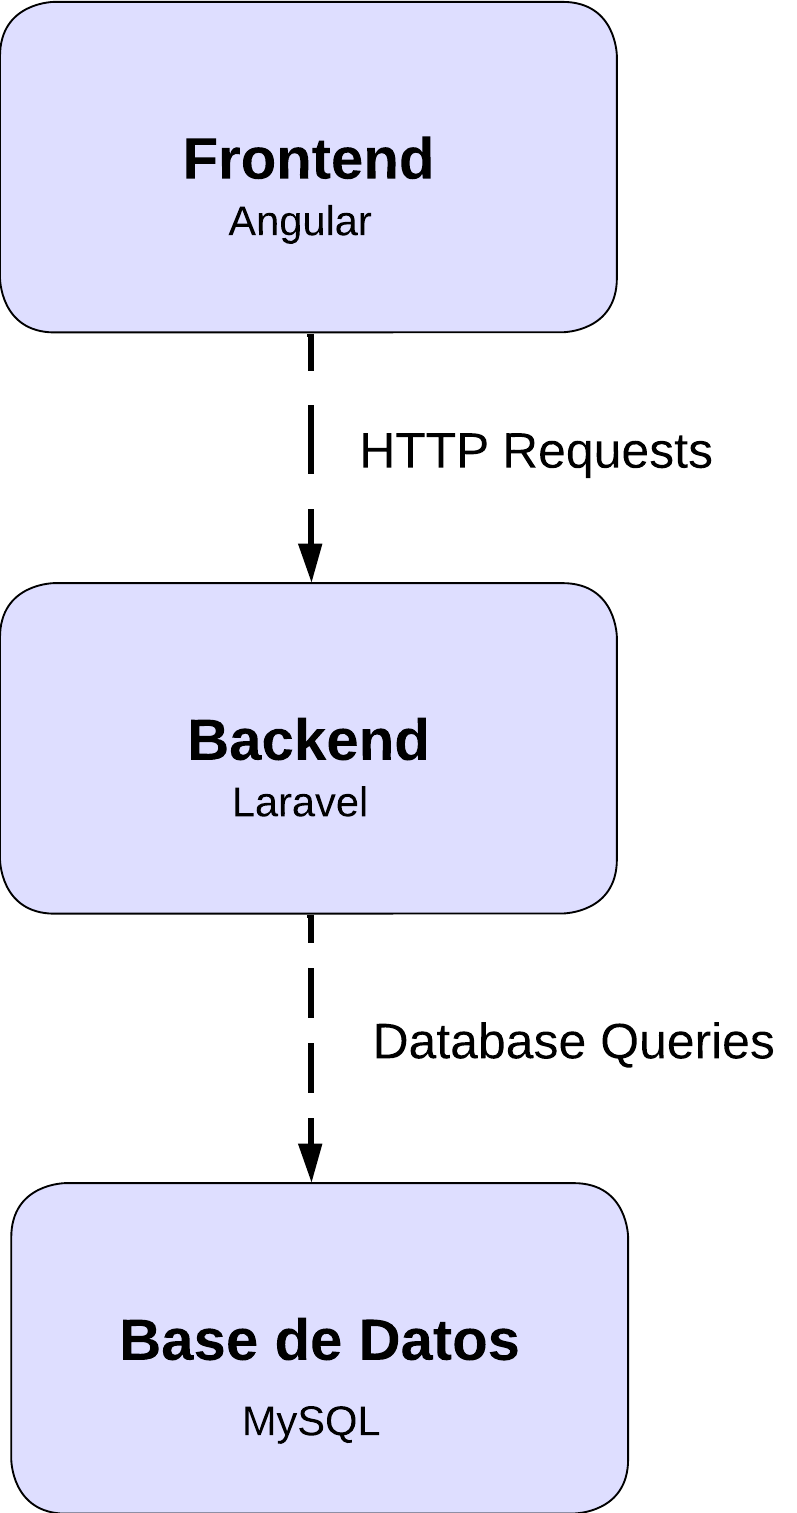
\includegraphics[scale=0.80]{./Images/diagramaTech.png}
\caption{Relación entre el Frontend (Angular), Backend (Laravel) y la Base de Datos (MySQL)}

\label{fig:fig1}

\end{center}
\end{figure}

El Frontend desarrollado en Angular envía peticiones HTTP al Backend, que utiliza el framework Laravel. Laravel gestiona las consultas de manera eficiente, permitiendo al backend comunicarse directamente con la base de datos MySQL, optimizando el acceso y la manipulación de los datos almacenados.

\section{Requisitos del proyecto}\label{sec:sec2.2}
En esta sección se detallan los requisitos que la aplicación debe cumplir para garantizar el éxito de su desarrollo:


\begin{itemize}
    \item La aplicación permitirá a los administradores gestionar el inventario de productos de pesca de forma integral, incluyendo la visualización en tiempo real del inventario y la capacidad de realizar actualizaciones en tiempo real.
    
    \item Se proporcionará una funcionalidad de ventas en línea que permita a los usuarios comprar productos de pesca directamente desde la aplicación web.
    
    \item Habrá un sistema de reservas de cebo integrado en la aplicación, que permitirá a los usuarios reservar cebo para su próxima salida de pesca.

    \item Los administradores podrán gestionar tanto los pedidos como las reservas de cebo. Cada vez que se realice un pedido o una reserva, se enviará un correo electrónico de confirmación tanto al cliente como al administrador.

    \item La aplicación contará con un sistema de autenticación de usuario para garantizar que solo los usuarios autorizados puedan acceder a determinadas funciones de la aplicación.

    \item El administrador podrá modificar la parte visual de la web, actualizando textos, imágenes y enlaces según sea necesario. Estos cambios permitirán reflejar nuevas ofertas, promociones o redirigir a los usuarios hacia secciones específicas del sitio web.

    \item La aplicación será diseñada con un enfoque en la seguridad y la usabilidad, asegurando que los datos de los usuarios estén protegidos y que la interfaz sea intuitiva y fácil de usar.
    
\end{itemize}

\chapter{Marco tecnológico}\label{cap:cap3}
El Marco Tecnológico establecido para el desarrollo del presente Trabajo Final de Máster (TFM) se fundamenta en la selección cuidadosa de herramientas y tecnologías que garanticen un rendimiento óptimo y una experiencia de usuario satisfactoria en el producto final. Por ello, se ha realizado un análisis exhaustivo de las diferentes opciones disponibles para cada capa del desarrollo (front-end, back-end y base de datos) y se han seleccionado aquellas que mejor se ajustan a los requisitos del proyecto.

\section{Base de datos: MySQL}\label{sec:sec3.1}

MySQL es un sistema de gestión de bases de datos relacional (SGBDR) de código abierto y ampliamente utilizado en el desarrollo web. Ofrece un rendimiento sólido, confiabilidad y escalabilidad, lo que lo convierte en una opción ideal para aplicaciones de todo tipo y tamaño. MySQL es una opción popular para el desarrollo de aplicaciones web debido a su facilidad de uso, rendimiento y amplia gama de características. \cite{mysql, elmasri, relational_vs_nosql}.

\vspace{0.5cm}

\begin{itemize}
    \item \textbf{Características principales de MySQL:}

    \begin{itemize}
    
    \item \textbf{Soporte para ACID:} Garantiza la integridad, consistencia, aislamiento y durabilidad de los datos. Las propiedades ACID son esenciales para garantizar la fiabilidad de las bases de datos y la seguridad de los datos.

    \item \textbf{Consultas SQL:} Permite manipular datos de manera eficiente mediante el lenguaje SQL. SQL es un lenguaje de consulta potente y versátil que permite realizar una amplia gama de operaciones sobre los datos.

    \item \textbf{Escalabilidad:} Puede manejar grandes volúmenes de datos y tráfico de usuarios. MySQL es una base de datos altamente escalable que puede adaptarse a las necesidades de aplicaciones web de todos los tamaños.

    \item \textbf{Seguridad:} Ofrece mecanismos de autenticación, autorización y cifrado de datos para proteger las bases de datos. La seguridad es un aspecto fundamental en el desarrollo de aplicaciones web, y MySQL ofrece una serie de características para proteger los datos de accesos no autorizados.
    
    \item \textbf{Amplia comunidad:} Cuenta con una gran comunidad de desarrolladores y una amplia gama de recursos disponibles. La gran comunidad de MySQL es un recurso valioso para los desarrolladores que necesitan ayuda o información.
    \end{itemize}

    \item \textbf{Beneficios de usar MySQL:}

    \begin{itemize}

    \item \textbf{Facilidad de uso:} MySQL es una base de datos relativamente fácil de aprender y usar, lo que la convierte en una buena opción para principiantes y desarrolladores con experiencia en otras tecnologías de bases de datos.
    
    \item \textbf{Rendimiento:} MySQL es una base de datos de alto rendimiento que puede manejar grandes volúmenes de datos y tráfico de usuarios.
    
    \item \textbf{Escalabilidad:} MySQL es una base de datos altamente escalable que puede adaptarse a las necesidades de aplicaciones web de todos los tamaños.
    
    \item \textbf{Seguridad:} MySQL ofrece una serie de características de seguridad para proteger los datos de accesos no autorizados.

    \item \textbf{Amplia comunidad:} La gran comunidad de MySQL es un recurso valioso para los desarrolladores que necesitan ayuda o información.
    
    \end{itemize}

    \item \textbf{Tabla comparativa con otras tecnologías de bases de datos:}

    \begin{longtable}[h]{ p{0.3\textwidth} | p{0.2\textwidth} | p{0.2\textwidth} | p{0.2\textwidth} |}
    \cline{2-4}
    & \cellcolor{naranja}{\color{blanco}\textbf{MySQL}} & \cellcolor{naranja}{\color{blanco}\textbf{PostgreSQL}} & \cellcolor{naranja}{\color{blanco}\textbf{MongoDB}} \\ \hline
    \endhead
    \cellcolor{naranja}{\color{blanco}\textbf{Modelo de datos}} & Relacional & Relacional & No relacional \\ \hline
    \cellcolor{naranja}{\color{blanco}\textbf{Curva de aprendizaje}} & Baja & Moderada & Baja \\ \hline
    \cellcolor{naranja}{\color{blanco}\textbf{Comunidad}} & Grande y activa & Grande y activa & Grande y activa \\ \hline
    \cellcolor{naranja}{\color{blanco}\textbf{Rendimiento}} & Alto & Alto & Escalable \\ \hline
    \cellcolor{naranja}{\color{blanco}\textbf{Adecuado para}} & Aplicaciones web transaccionales & Aplicaciones web complejas con consultas complejas & Aplicaciones web NoSQL \\ \hline
    
    \caption{Tabla comparativa con otras tecnologías de base de datos}
    \label{tab:otras-soluciones}
    \end{longtable}

    \item \textbf{Casos de uso de MySQL:}

    MySQL es una opción popular para el desarrollo de una amplia gama de aplicaciones web, incluyendo:
    
    \begin{itemize}

    \item \textbf{Tiendas online:} MySQL es una buena opción para almacenar datos de productos, pedidos y clientes.

    \item \textbf{Aplicaciones web de redes sociales:} MySQL puede usarse para almacenar datos de perfiles de usuarios, publicaciones, mensajes y otros datos relacionados con las redes sociales.

    \item \textbf{Aplicaciones web de blogs:} MySQL puede usarse para almacenar datos de entradas de blog, comentarios y otros datos relacionados con los blogs.

    \item \textbf{Aplicaciones web de gestión de proyectos:} MySQL puede usarse para almacenar datos de proyectos, tareas, usuarios y otros datos relacionados con la gestión de proyectos.

    \end{itemize}
\end{itemize}
\section{Back-end: Laravel}\label{sec:sec3.2}

Laravel es un framework PHP de código abierto para el desarrollo web back-end. Proporciona una estructura robusta y elegante para crear aplicaciones web modernas y escalables. Laravel es conocido por su sintaxis elegante, su amplio conjunto de características y su gran comunidad de desarrolladores \cite{laravel, stauffer}.

\vspace{0.5cm}

\begin{itemize}
    \item \textbf{Características principales de Laravel:}
    \begin{itemize}

    \item \textbf{Arquitectura MVC:} Laravel sigue el patrón de diseño MVC (Modelo-Vista-Controlador), separando la lógica de la aplicación en tres capas bien definidas. Esto promueve la separación de responsabilidades, facilita el desarrollo y mantenimiento del código y mejora la testabilidad.

    \item \textbf{Ruteo Elocuente:} Laravel proporciona un sistema de ruteo flexible y fácil de usar que le permite definir fácilmente las rutas de su aplicación y asociarlas con controladores específicos.

    \item \textbf{Eloquent ORM:} Laravel incluye un Object-Relational Mapper (ORM) llamado Eloquent que facilita la interacción con bases de datos relacionales. Eloquent le permite trabajar con objetos PHP en lugar de consultas SQL, lo que simplifica el desarrollo y reduce la cantidad de código necesario.

    \item \textbf{Artisan:} Laravel incluye una herramienta de línea de comandos llamada Artisan que le permite realizar tareas comunes de administración de aplicaciones, como crear migraciones, sembrar bases de datos y ejecutar pruebas.

    \item \textbf{Seguridad:} Laravel incluye una serie de características de seguridad integradas que ayudan a proteger su aplicación de ataques comunes, como ataques de inyección de SQL y ataques de sitios cruzados (XSS).

    \item \textbf{Comunidades y recursos:} Laravel cuenta con una comunidad grande y activa de desarrolladores. Hay una gran cantidad de recursos disponibles, como documentación oficial, tutoriales, foros y paquetes de terceros
    
    \end{itemize}

    \item \textbf{Beneficios de usar Laravel:}
    \begin{itemize}

    \item \textbf{Desarrollo rápido y escalable:} Laravel proporciona una estructura robusta y herramientas que facilitan el desarrollo de aplicaciones web complejas y escalables.
    
    \item \textbf{Código limpio y mantenible:} La sintaxis elegante de Laravel y su enfoque en la separación de responsabilidades promueven la creación de código limpio y fácil de mantener.

    \item \textbf{Seguridad mejorada:} Las características de seguridad integradas de Laravel ayudan a proteger su aplicación de ataques comunes.

    \item \textbf{Gran comunidad y recursos:} La gran comunidad de Laravel y la amplia gama de recursos disponibles facilitan encontrar ayuda y resolver problemas.

    \end{itemize}

     \item \textbf{Tabla comparativa con otras tecnologías back-end:}
     
    \begin{longtable}[h]{ p{0.3\textwidth} | p{0.2\textwidth} | p{0.2\textwidth} | p{0.2\textwidth} |}
    \cline{2-4}
    & \cellcolor{naranja}{\color{blanco}\textbf{Laravel}} & \cellcolor{naranja}{\color{blanco}\textbf{Django}} & \cellcolor{naranja}{\color{blanco}\textbf{Ruby on Rails}} \\ \hline
    \endhead
    \cellcolor{naranja}{\color{blanco}\textbf{Lenguaje de programación}} & PHP & Python & Ruby \\ \hline
    \cellcolor{naranja}{\color{blanco}\textbf{Paradigma de programación}} & MVC & MVC & MVC \\ \hline
    \cellcolor{naranja}{\color{blanco}\textbf{Estructura}} & Basada en rutas y controladores & Basada en vistas y URLconf & Basada en rutas y controladores \\ \hline
    \cellcolor{naranja}{\color{blanco}\textbf{Curva de aprendizaje}} & Moderada & Moderada & Moderada \\ \hline
    \cellcolor{naranja}{\color{blanco}\textbf{Comunidad}} & Grande y activa & Grande y activa & Grande y activa \\ \hline
    \cellcolor{naranja}{\color{blanco}\textbf{Rendimiento}} & Alto & Alto & Alto \\ \hline
    \cellcolor{naranja}{\color{blanco}\textbf{Adecuado para}} & Aplicaciones web complejas y escalables & Aplicaciones web complejas y escalables & Aplicaciones web complejas y escalables \\ \hline
    
    \caption{Tabla comparativa con otras tecnologías back-end}
    \label{tab:otras-soluciones}
    \end{longtable}
    
     \item \textbf{Casos de uso de Laravel:}

    Laravel es una opción ideal para el desarrollo de una amplia variedad de aplicaciones web back-end, incluyendo:
    
     \begin{itemize}

    \item \textbf{Aplicaciones web empresariales:} CRM, ERP, gestión de proyectos, etc.

    \item \textbf{Aplicaciones web de comercio electrónico:} Tiendas online, plataformas de pago, etc.

    \item \textbf{Aplicaciones web API:} API RESTful para proporcionar datos a aplicaciones móviles o front-end web.

    \item \textbf{Aplicaciones web de una sola página (SPA):} Aplicaciones web que se cargan una sola vez y que navegan entre diferentes vistas sin necesidad de recargar la página.

    \item \textbf{Aplicaciones web progresivas (PWA):} Aplicaciones web que combinan las características de las aplicaciones web tradicionales con las de las aplicaciones móviles.
    
    \end{itemize}
\end{itemize}
\section{Front-end: Angular}\label{sec:sec3.3}

Angular es un framework de desarrollo web front-end de código abierto y mantenido por Google. Proporciona una estructura robusta y modular para construir aplicaciones web escalables y de alto rendimiento. Su arquitectura MVC facilita la organización del código y promueve la mantenibilidad a largo plazo \cite{angular, angular_development}.

\vspace{0.5cm}

\begin{itemize}
    \item \textbf{Características principales de Angular:}

    \begin{itemize}

    \item \textbf{Arquitectura MVC:} Separa la aplicación en tres capas: modelo, vista y controlador, promoviendo la separación de responsabilidades y facilitando el desarrollo y mantenimiento del código.

    \item \textbf{Encapsulamiento de componentes:} Permite crear componentes reutilizables y altamente personalizables, lo que facilita el desarrollo de interfaces complejas y la reutilización de código.

    \item \textbf{Data binding:} Simplifica la sincronización entre los datos del modelo y la vista, proporcionando una experiencia de usuario fluida y reactiva. Esto significa que cualquier cambio en los datos del modelo se reflejará automáticamente en la interfaz de usuario, sin necesidad de escribir código adicional.

    \item \textbf{Directivas:} Ofrecen funcionalidades predefinidas para manipular el DOM y mejorar la interacción con el usuario. Las directivas permiten extender la funcionalidad HTML y crear elementos personalizados.

    \item \textbf{Herramientas de desarrollo:} Incluye un conjunto completo de herramientas para el desarrollo, testing y despliegue de aplicaciones Angular. Estas herramientas facilitan el trabajo de los desarrolladores y permiten crear aplicaciones de alta calidad.

    \end{itemize}

    \item \textbf{Beneficios de usar Angular:}

    \begin{itemize}

    \item \textbf{Desarrollo rápido y escalable:} Angular proporciona una estructura robusta y herramientas que facilitan el desarrollo de aplicaciones web complejas y escalables.

    \item \textbf{Interfaces de usuario dinámicas y reactivas:} La arquitectura MVC y el data binding de Angular permiten crear interfaces de usuario dinámicas y reactivas que responden a los cambios en los datos de forma inmediata.

    \item \textbf{Código reutilizable y mantenible:} El encapsulamiento de componentes y la separación de responsabilidades promueven la creación de código reutilizable y fácil de mantener.

    \item \textbf{Gran comunidad y recursos disponibles:} Angular cuenta con una gran comunidad de desarrolladores y una amplia gama de recursos disponibles, lo que facilita encontrar ayuda y resolver problemas.

     \end{itemize}

     \item \textbf{Tabla comparativa con otras tecnologías front-end:}

    \begin{longtable}[h]{ p{0.3\textwidth} | p{0.2\textwidth} | p{0.2\textwidth} | p{0.2\textwidth} |}
    \cline{2-4}
    & \cellcolor{naranja}{\color{blanco}\textbf{Angular}} & \cellcolor{naranja}{\color{blanco}\textbf{React}} & \cellcolor{naranja}{\color{blanco}\textbf{Vue.js}} \\ \hline
    \endhead
    \cellcolor{naranja}{\color{blanco}\textbf{Estructura}} & MVC & Componentes & Componentes \\ \hline
    \cellcolor{naranja}{\color{blanco}\textbf{Curva de aprendizaje}} & Moderada & Moderada & Baja \\ \hline
    \cellcolor{naranja}{\color{blanco}\textbf{Comunidad}} & Grande y activa & Grande y activa & Grande y activa \\ \hline
    \cellcolor{naranja}{\color{blanco}\textbf{Rendimiento}} & Alto & Alto & Alto \\ \hline
    \cellcolor{naranja}{\color{blanco}\textbf{Adecuado para}} & Aplicaciones web complejas y escalables & Aplicaciones web de una sola página y dinámicas & Aplicaciones web pequeñas y medianas \\ \hline
    
    \caption{Tabla comparativa con otras tecnologías front-end}
    \label{tab:otras-soluciones}
    \end{longtable}
    
     \item \textbf{Casos de uso de Angular:}
    
     Angular es una opción ideal para el desarrollo de aplicaciones web complejas y escalables que requieren interfaces de usuario dinámicas y reactivas. Algunos ejemplos de casos de uso de Angular incluyen:

      \begin{itemize}

    \item \textbf{Aplicaciones web empresariales:} CRM, ERP, gestión de proyectos, etc.

    \item \textbf{Aplicaciones web de comercio electrónico:} Tiendas online, plataformas de pago, etc.

    \item \textbf{Aplicaciones web de una sola página (SPA):} Aplicaciones web que se cargan una sola vez y que navegan entre diferentes vistas sin necesidad de recargar la página.

    \item \textbf{Aplicaciones web progresivas (PWA):} Aplicaciones web que combinan las características de las aplicaciones web tradicionales con las de las aplicaciones móviles.

    \end{itemize}
\end{itemize}

\chapter{Metodología}\label{cap:cap4}
Para afrontar este Trabajo de Fin de Máster (TFM), se ha decidido adoptar una metodología ágil que se ajusta a las exigencias dinámicas del proyecto. Esta elección se sustenta en la necesidad de asegurar una ejecución eficiente, flexible y orientada a la obtención de resultados concretos.

\vspace{0.5cm}

La metodología ágil se caracteriza por su enfoque iterativo e incremental, lo que permite dividir el proyecto en etapas o iteraciones manejables. Cada iteración se centra en un conjunto específico de tareas y objetivos, facilitando así un progreso continuo y una rápida adaptación a los cambios del entorno. Asimismo, fomenta una estrecha colaboración con los interesados y la posibilidad de realizar ajustes según las necesidades emergentes.

\vspace{0.5cm}

Es bien sabido que este enfoque ágil es altamente efectivo en proyectos de desarrollo de software, como el presente, debido a su capacidad para mejorar la gestión del proyecto. En este tipo de iniciativas, la comunicación fluida, la capacidad de adaptación y la entrega incremental de funcionalidades son aspectos cruciales. Todos estos aspectos pueden ser alcanzados eficazmente mediante la implementación de una metodología ágil.

\vspace{0.5cm}

A continuación, se detallará la gestión del proyecto y las herramientas utilizadas para su ejecución efectiva.

\section{Gestión del proyecto}\label{sec:apartado}

Para gestionar eficazmente el proyecto, se han empleado herramientas alineadas con la metodología ágil Scrum \cite{schwaber2017}. A partir de los requisitos del proyecto, se ha elaborado un Product Backlog que incluye las Historias de Usuario \cite{cohn2004}, delineando así las necesidades específicas desde la perspectiva del cliente o usuario final. En lugar de detallar exhaustivamente especificaciones técnicas, las Historias de Usuario se centran en los objetivos y expectativas de los usuarios de la aplicación.

\vspace{0.5cm}

La planificación se ha estructurado en diferentes Sprints, cada uno con las tareas necesarias para avanzar hacia el objetivo final: la aplicación web. La conclusión exitosa de estos Sprints conducirá al resultado deseado.

\vspace{0.5cm}

En la sección \textcolor{naranja}{sección 4.1.1 - Historias de usuario}, se presenta en detalle esta hoja de ruta, que guiará la creación de las funcionalidades requeridas por los usuarios, abordando así las necesidades específicas del proyecto.


\subsection{Historias de usuario}\label{subsec4.1.1}

En base a los requisitos de la aplicación se han identificado las siguientes historias de usuario:



\begin{table}[H]
  \centering
  \renewcommand{\arraystretch}{1.5}
  \begin{tabular}{|p{0.3\textwidth}|p{0.3\textwidth}|p{0.3\textwidth}|}
    \hline
    \multicolumn{3}{|l|}{\cellcolor{OrangeVIU}\textcolor{white}{\textbf{(H1) Historia de usuario 1: Creación BBDD}}} \\
    \hline
    \multicolumn{3}{|p{\dimexpr0.9\linewidth+2\tabcolsep+2\arrayrulewidth}|}{{\textbf{\textcolor{naranja}{Descripción: }}}Crear una base de datos desde cero para almacenar datos esenciales del sistema.} \\
    \hline
    \multicolumn{3}{|p{\dimexpr0.9\linewidth+2\tabcolsep+2\arrayrulewidth}|}{{\textbf{\textcolor{naranja}{Validación: }} Se debe verificar que todas las tablas requeridas hayan sido creadas correctamente en la base de datos, asegurando que cada tabla contenga las columnas necesarias y cumpla con las restricciones de integridad definidas. }} \\
    \hline
    {\textbf{\textcolor{naranja}{Prioridad }}}  & {\textbf{\textcolor{naranja}{Estimación }}}  & {\textbf{\textcolor{naranja}{Dependencia }}}  \\
    \hline
    1 &  30h &  Ninguna \\
    \hline
  \end{tabular}
  \caption{(H1) Historia de usuario 1 - Creación BBDD}
  \label{table:H1}
\end{table}


    Esta historia de usuario representa una de las primeras tareas clave en el desarrollo del sistema, que es la creación de la base de datos (BBDD). El desarrollo se ha gestionado mediante un enfoque iterativo y basado en Scrum. La creación de la base de datos es un paso crucial en la arquitectura de la aplicación, ya que asegura que toda la información requerida por el sistema esté correctamente estructurada.

    \vspace{0.5cm}
    
    La validación de esta tarea se llevará a cabo al finalizar el Sprint correspondiente, verificando la integridad de las tablas y asegurando que se cumplan los requisitos establecidos en las historias de usuario dependientes. Esta historia se considera de alta prioridad debido a su impacto en las demás funcionalidades del sistema.


\begin{table}[H]
  \centering
  \renewcommand{\arraystretch}{1.5}
  \begin{tabular}{|p{0.3\textwidth}|p{0.3\textwidth}|p{0.3\textwidth}|}
    \hline
    \multicolumn{3}{|l|}{\cellcolor{OrangeVIU}\textcolor{white}{\textbf{(H2) Historia de usuario 2: Introducir nuevo producto}}} \\
    \hline
    \multicolumn{3}{|p{\dimexpr0.9\linewidth+2\tabcolsep+2\arrayrulewidth}|}{{\textbf{\textcolor{naranja}{Descripción: }}}Permitir a los usuarios agregar un nuevo producto al sistema, proporcionando información detallada como nombre, descripción, precio y categoría.} \\
    \hline
    \multicolumn{3}{|p{\dimexpr0.9\linewidth+2\tabcolsep+2\arrayrulewidth}|}{{\textbf{\textcolor{naranja}{Validación: }} Verificar que el nuevo producto se haya añadido correctamente a la base de datos, con todos los campos necesarios completos y sin errores de duplicación. }} \\
    \hline
    {\textbf{\textcolor{naranja}{Prioridad }}}  & {\textbf{\textcolor{naranja}{Estimación }}}  & {\textbf{\textcolor{naranja}{Dependencia }}}  \\
    \hline
    1 &  10h &  1 \\
    \hline
  \end{tabular}
  \caption{(H2) Historia de usuario 2 - Introducir nuevo producto}
  \label{table:H2}
\end{table}


    Esta historia de usuario aborda la funcionalidad esencial para el administrador de la aplicación, permitiéndole gestionar el catálogo de productos en el sistema. El enfoque Scrum nos ha permitido dividir esta tarea en sub-actividades como el diseño de la interfaz de usuario, la conexión con la base de datos y la validación de datos.

    \vspace{0.5cm}
    
    Durante el Sprint, se llevarán a cabo pruebas unitarias y de integración para garantizar que el sistema maneje correctamente la introducción de nuevos productos y que los datos se guarden de manera segura en la base de datos. Esta tarea es crítica para garantizar que el inventario se mantenga actualizado en todo momento, siendo una funcionalidad recurrente en futuras iteraciones.


\vspace{0.5cm}
\vspace{0.5cm}
Después de presentar las primeras historias de usuario clave para el desarrollo del sistema, el resto de las historias de usuario, que detallan el resto de funcionalidades se encuentran recogidas en el \textcolor{naranja}{Anexo I: Historias de usuario}. Estas historias son igualmente importantes para la correcta implementación y funcionamiento de la plataforma, y abarcan aspectos como la gestión avanzada del inventario, la autenticación de usuarios y la reserva de productos. Para mayor detalle, se pueden consultar todas las tablas en el mencionado anexo.


\subsection{Mapa de historias de usuario}\label{subsec4.1.2}

Después de definir las historias de usuario, se elabora un mapa que muestra en detalle cada una de estas historias y el Sprint en el que serán ejecutadas. 

\begin{figure}[H]
\begin{center}
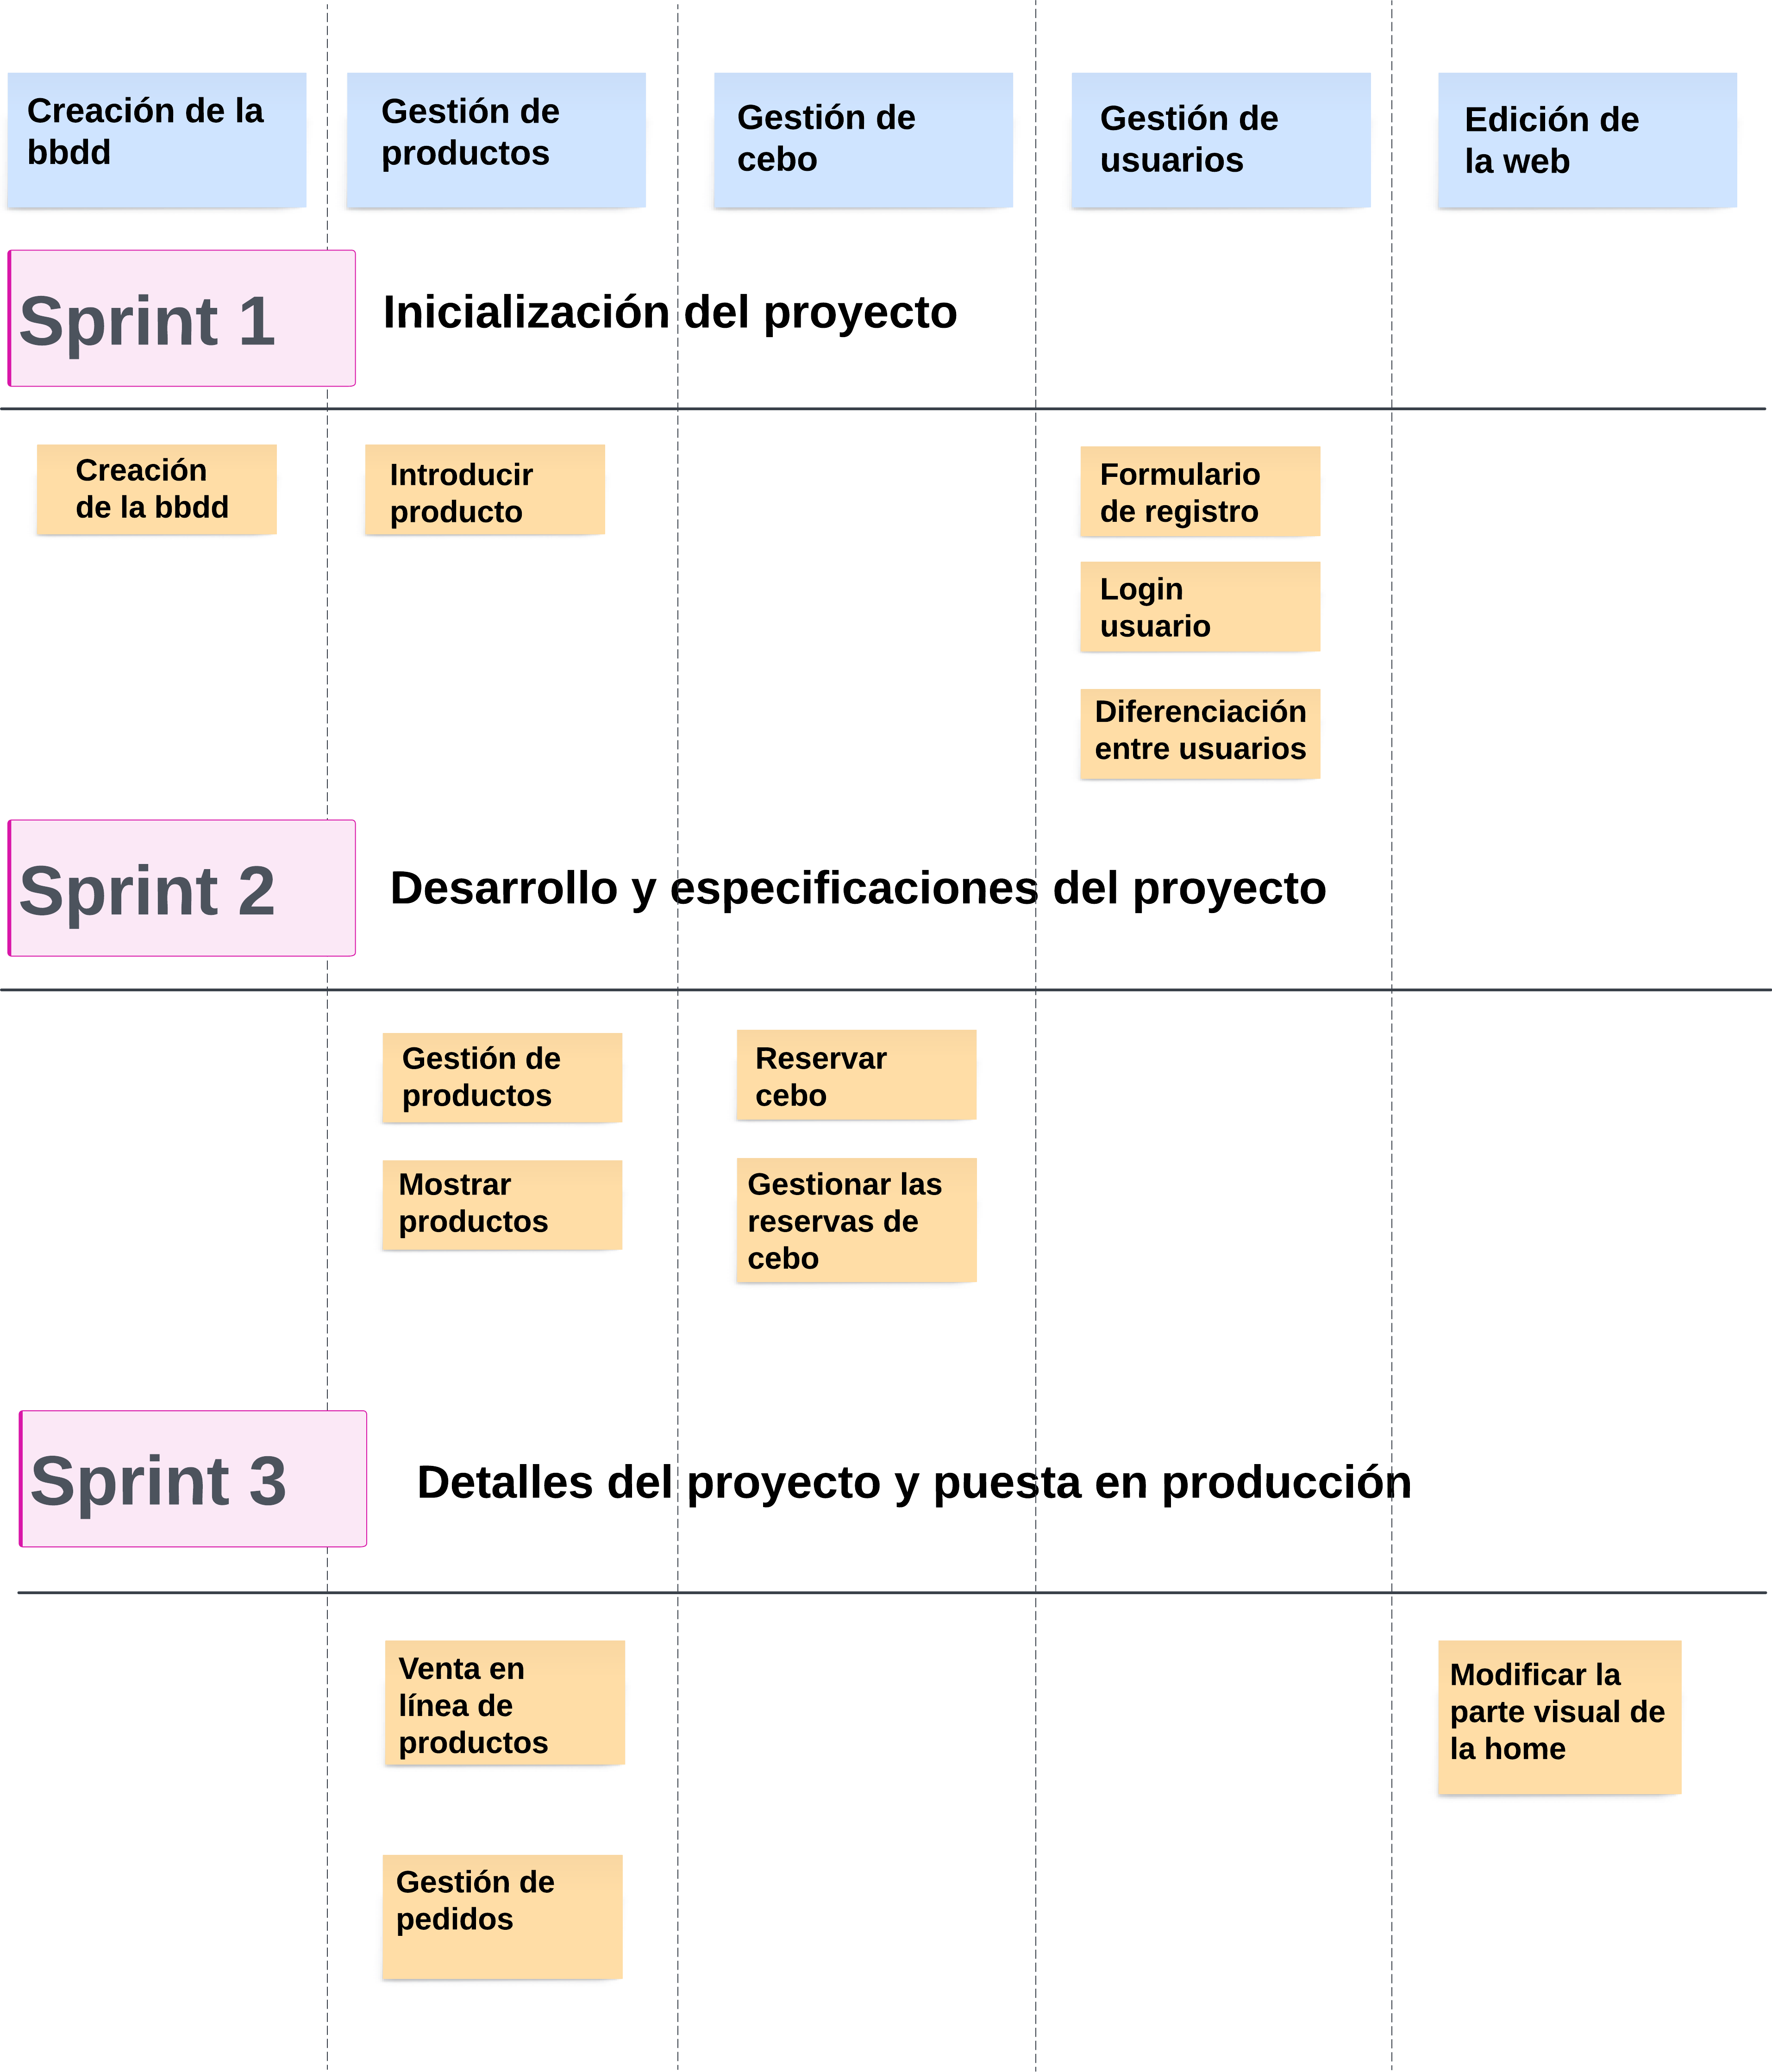
\includegraphics[scale=0.11]{./Images/MapaHistoriasUsuario.png}
\caption{Mapa de historias de usuario}

\label{fig:fig1}

\end{center}
\end{figure}

\subsection{Sprints}\label{subsec4.1.3}

A partir del mapa de historias de usuario se han generado 3 Sprints para llevar a cabo todas las tareas.

\begin{itemize}
    \item \textbf{Sprint 1: }Se comenzará con la creación de la base de datos, la funcionalidad para introducir un producto y la implementación del registro de usuarios. Además, se desarrollará el sistema de login y se diferenciarán los roles de usuario, especialmente entre administrador y usuarios regulares.

    \item \textbf{Sprint 2: }Se procederá con la gestión de productos, la funcionalidad para mostrar productos organizados por categorías y el sistema de reservas de cebo. También se implementará la gestión de las reservas de cebo por parte del administrador, garantizando que estén listas para la fecha de recogida.
    
    \item \textbf{Sprint 3: }Se desarrollará la venta en línea de productos, incluyendo la adición de productos al carrito y la gestión de pedidos. Además, se implementará la funcionalidad para modificar la parte visual de la página de inicio (home).
    
\end{itemize}

\section{Modelos para la interfaz - Mockup}\label{sec:apartado}
En este apartado, nos adentraremos en el proceso de diseño de la interfaz de usuario para nuestra aplicación. La interfaz de usuario desempeña un papel crucial en la experiencia del usuario, ya que actúa como el punto de interacción principal entre los usuarios y la funcionalidad ofrecida por la aplicación. Para garantizar una experiencia de usuario intuitiva y atractiva, es fundamental desarrollar una interfaz bien diseñada que refleje las necesidades y expectativas de nuestros usuarios.

\vspace{0.5cm}

Para alcanzar este objetivo, hemos empleado una metodología centrada en el usuario que comienza con la creación de modelos para la interfaz, conocidos como mockups. Estos mockups proporcionan representaciones visuales de la estructura y el diseño de la interfaz para diferentes tipos de usuarios, incluidos clientes y administradores. Además de las vistas de cliente y administrador, hemos agregado la vista de registro de usuario y login. Es importante destacar que el proceso de login será el mismo tanto para los clientes como para los administradores, proporcionando una experiencia unificada para todos los usuarios. En la vista del cliente, nos enfocaremos en proporcionar una experiencia de compra fluida y agradable, mientras que en la vista del administrador nos concentraremos en herramientas de gestión y control para administrar eficientemente la plataforma.

\subsection{Mockup registro y login}\label{subsec4.2.1}

En la Figura 4.2 se muestra la pantalla de registro de usuarios. Esta interfaz permite a los usuarios crear una cuenta en nuestra plataforma proporcionando la información necesaria de manera clara y sencilla.

\begin{figure}[H]
\begin{center}
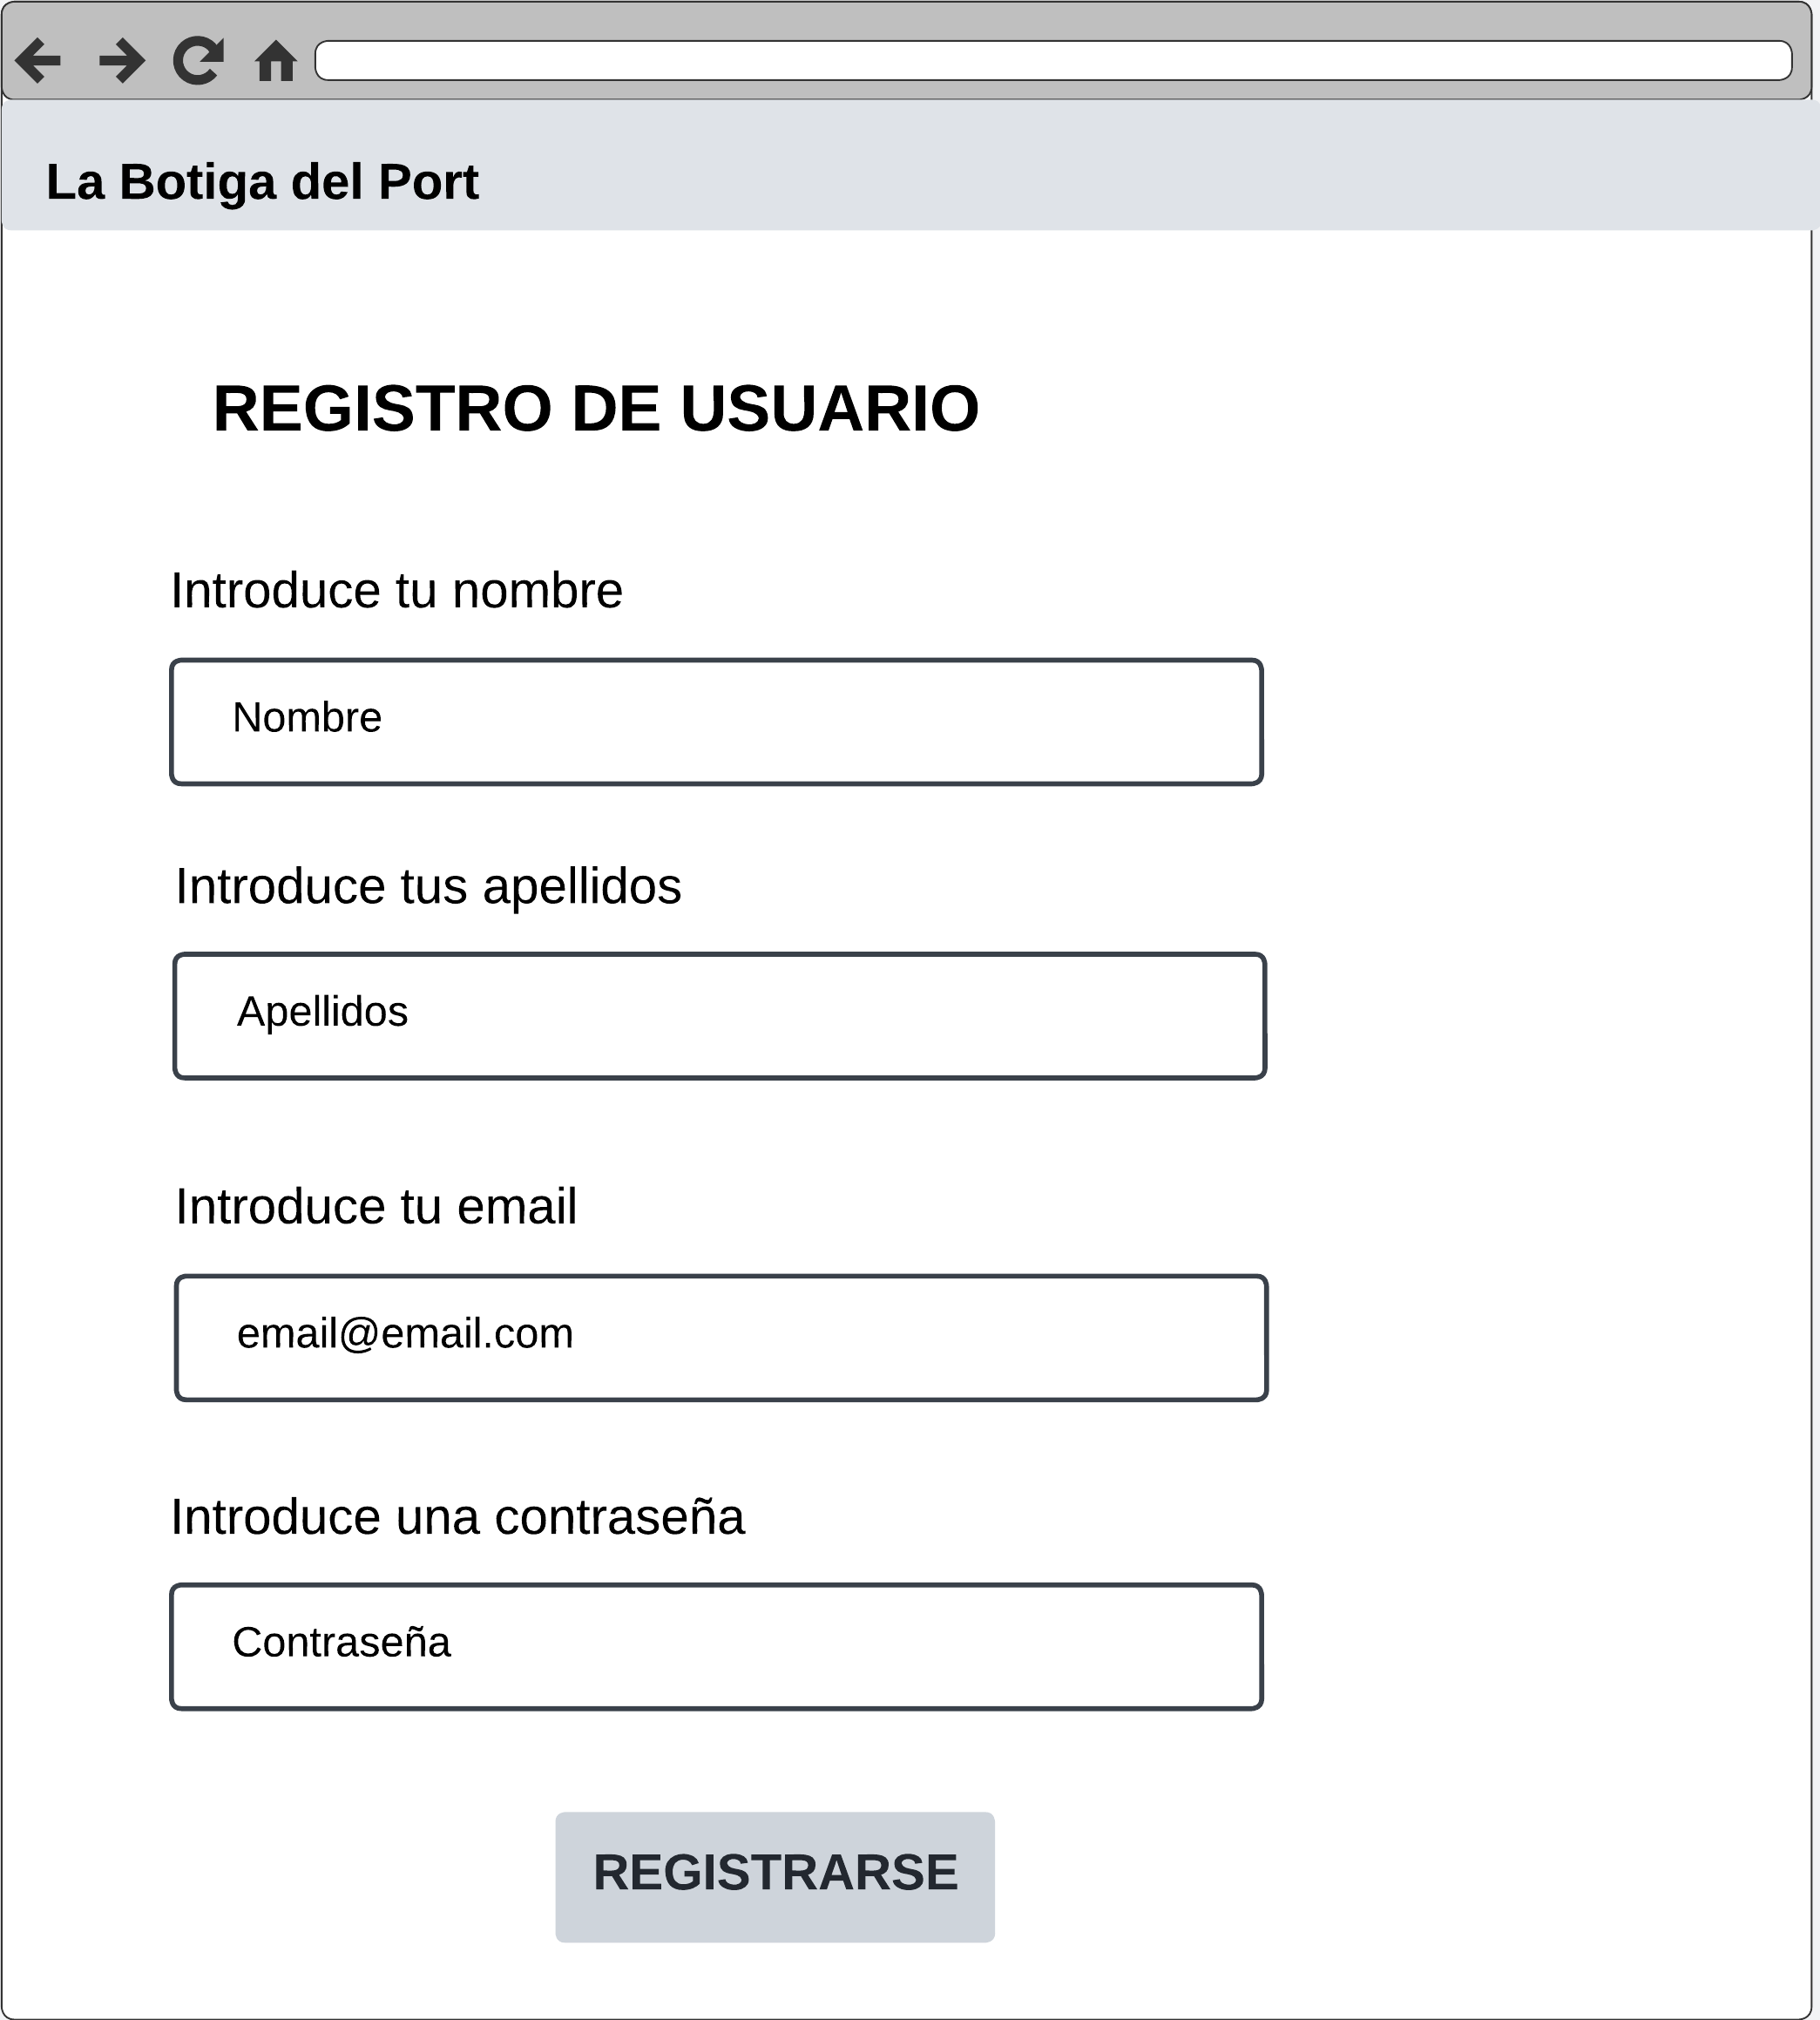
\includegraphics[scale=0.5]{./Images/registro.png}
\caption{Modelo de registro.} Fuente: Elaboración propia.

\label{fig:fig2}

\end{center}
\end{figure}


La Figura 4.3 presenta la pantalla de inicio de sesión. Aquí, los usuarios pueden acceder a sus cuentas ingresando su correo electrónico y contraseña de forma segura.


\begin{figure}[H]
\begin{center}
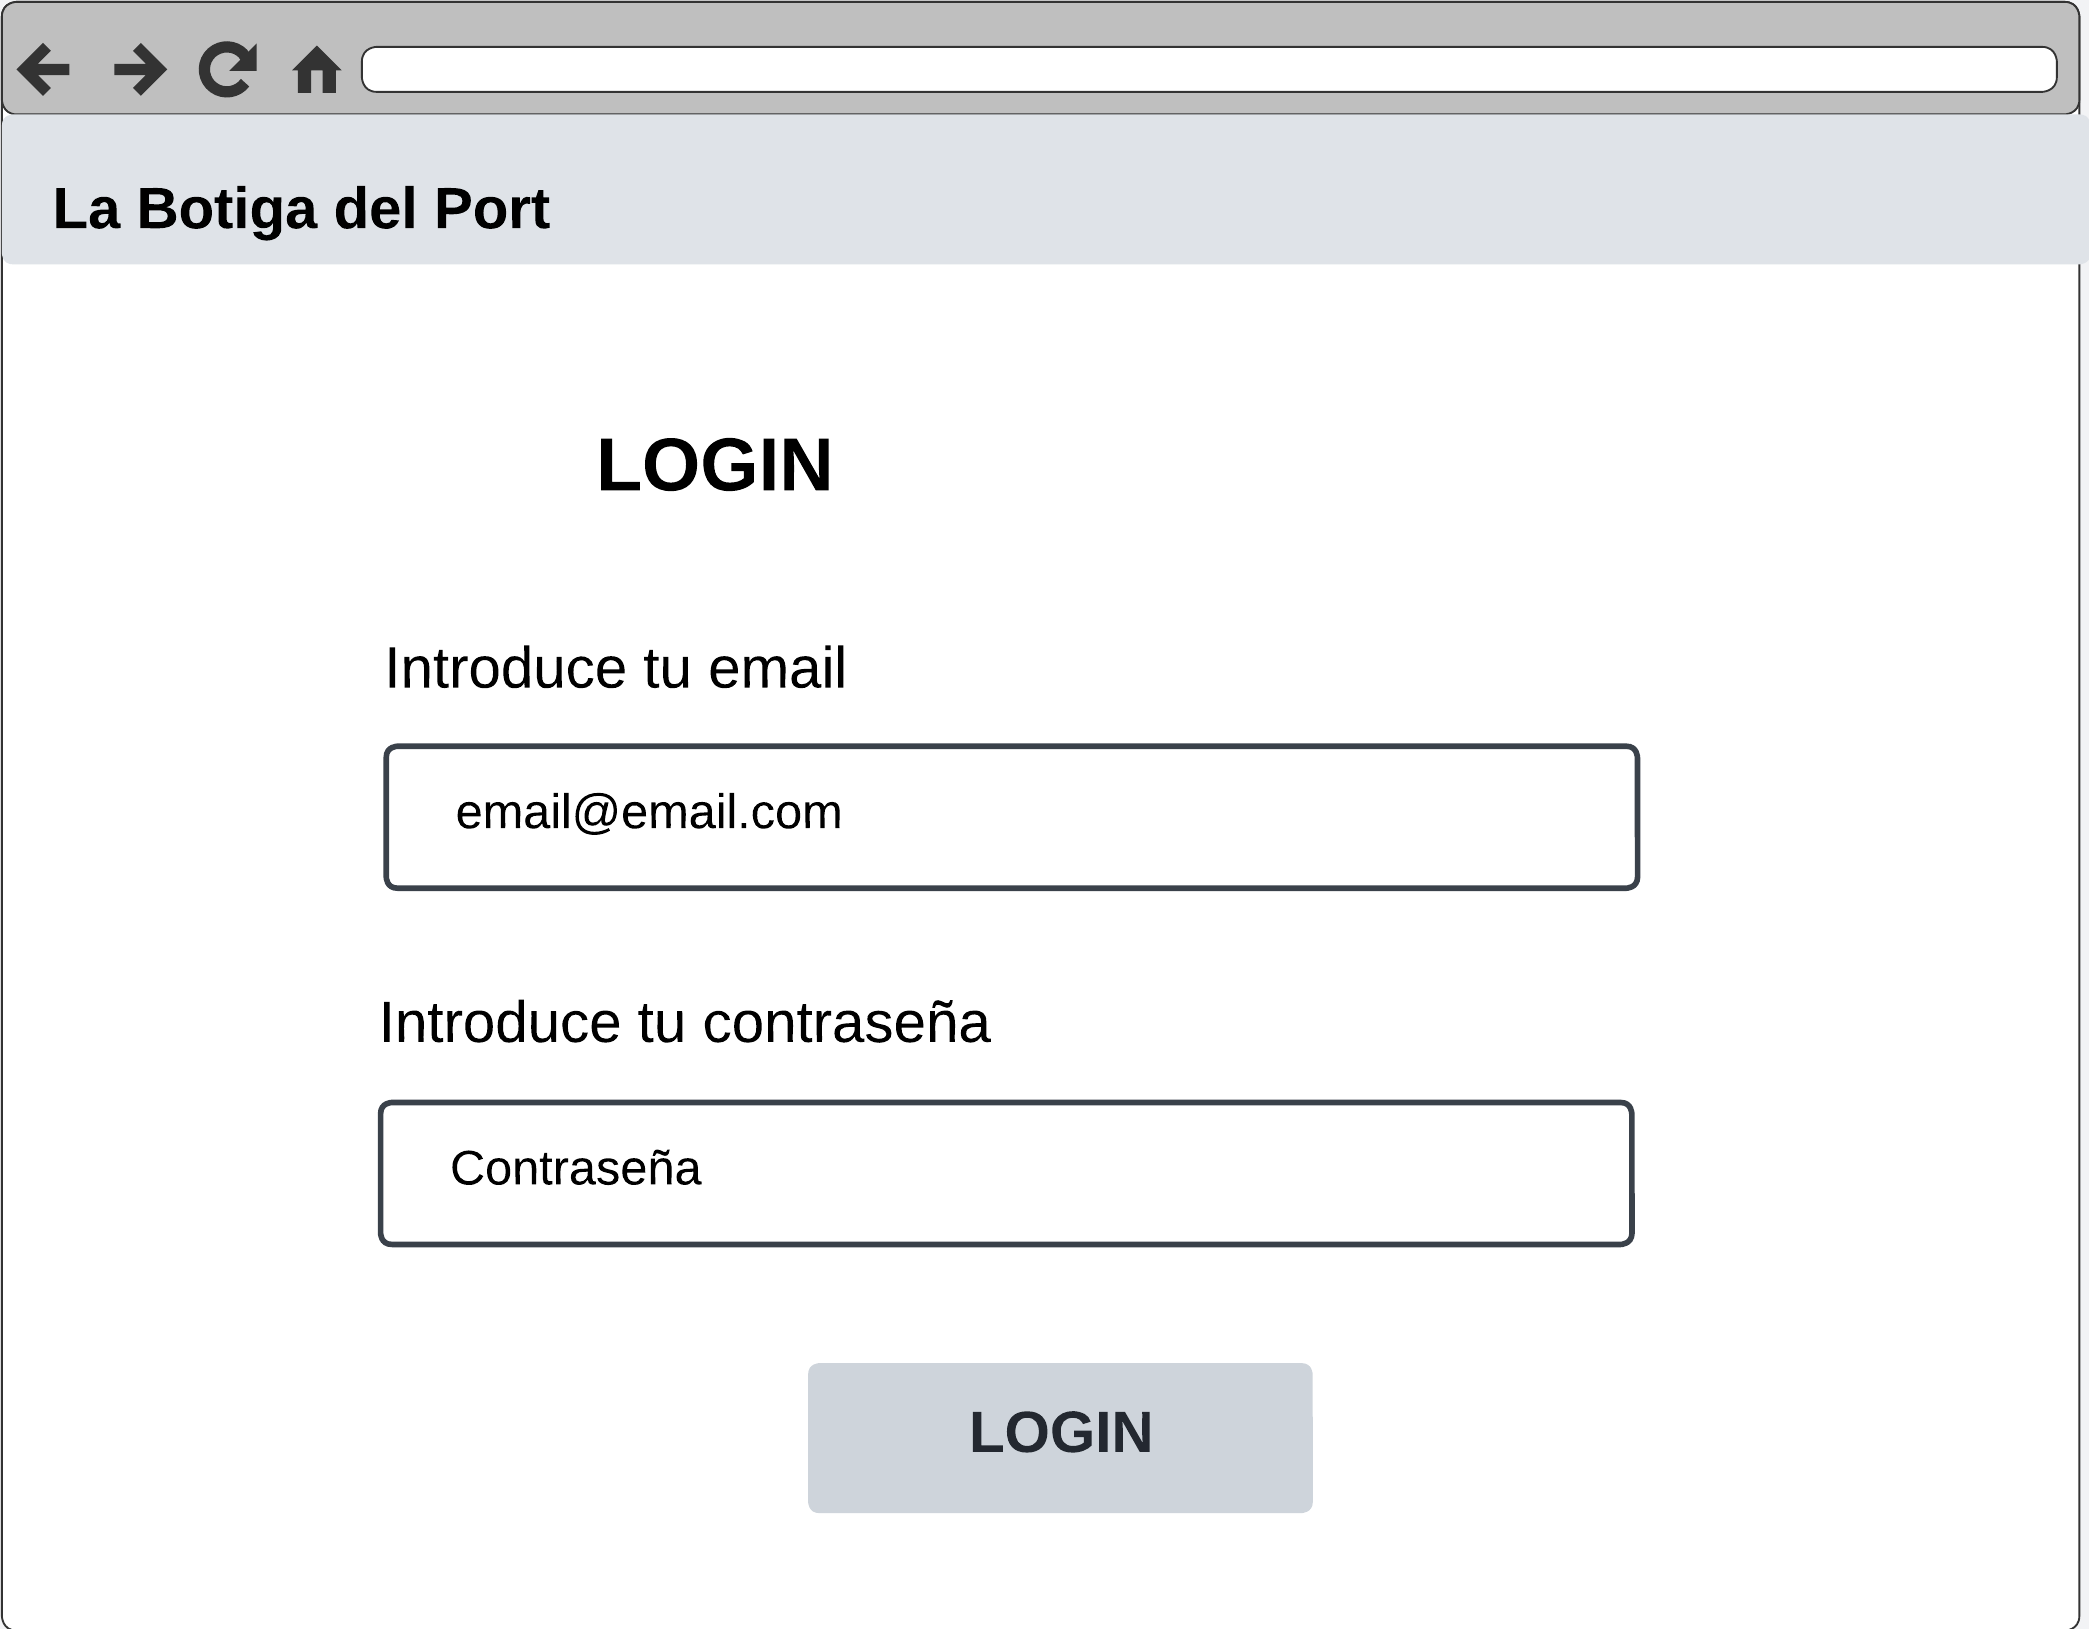
\includegraphics[scale=0.5]{./Images/login.png}
\caption{Modelo de Login.} Fuente: Elaboración propia.

\label{fig:fig3}

\end{center}
\end{figure}

\subsection{Mockup para el cliente}\label{subsec4.2.2}

La Figura 4.4 muestra una de las páginas principales de productos de nuestra aplicación. En esta vista, los usuarios pueden explorar una selección de productos y acceder al detale de cada uno de los productos. 

\begin{figure}[H]
\begin{center}
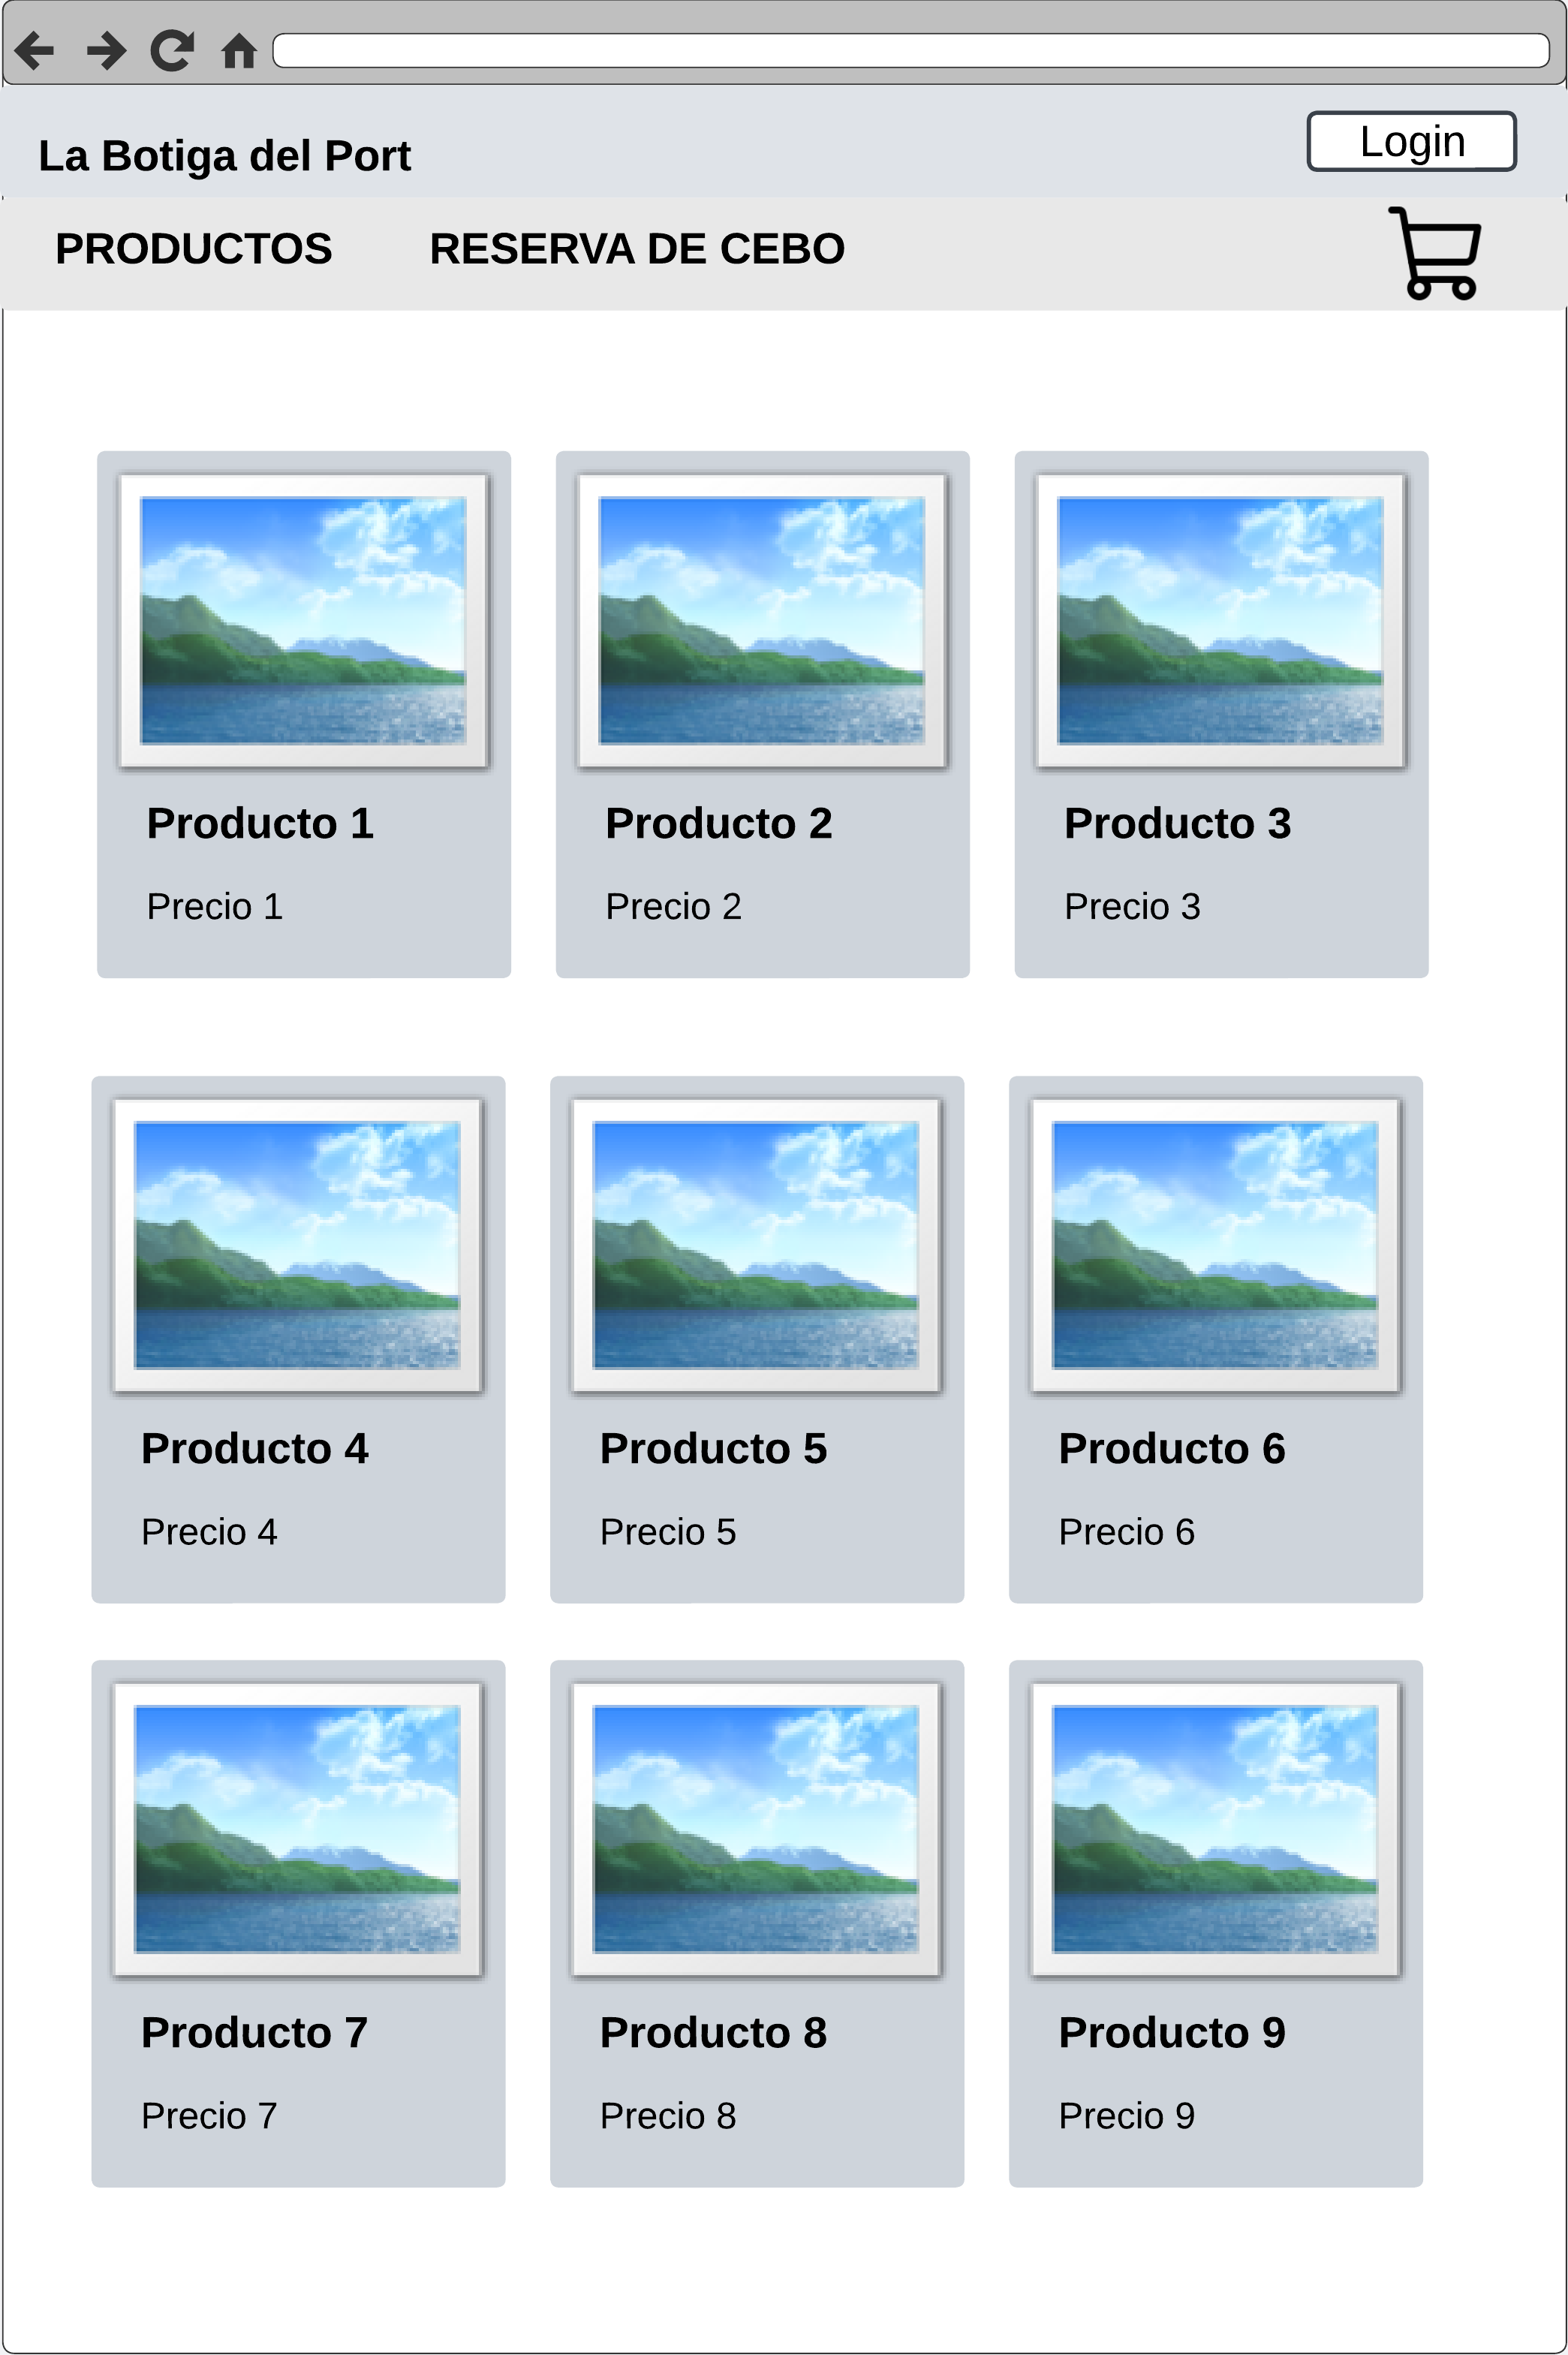
\includegraphics[scale=0.5]{./Images/productos.png}
\caption{Modelo de cliente - Página de productos.} Fuente: Elaboración propia.

\label{fig:fig4}

\end{center}
\end{figure}

En la Figura 4.5 se presenta el detalle del producto. Esta interfaz proporciona a los usuarios información detallada sobre un producto específico, incluyendo su descripción, precio y opciones de compra. 

\begin{figure}[H]
\begin{center}
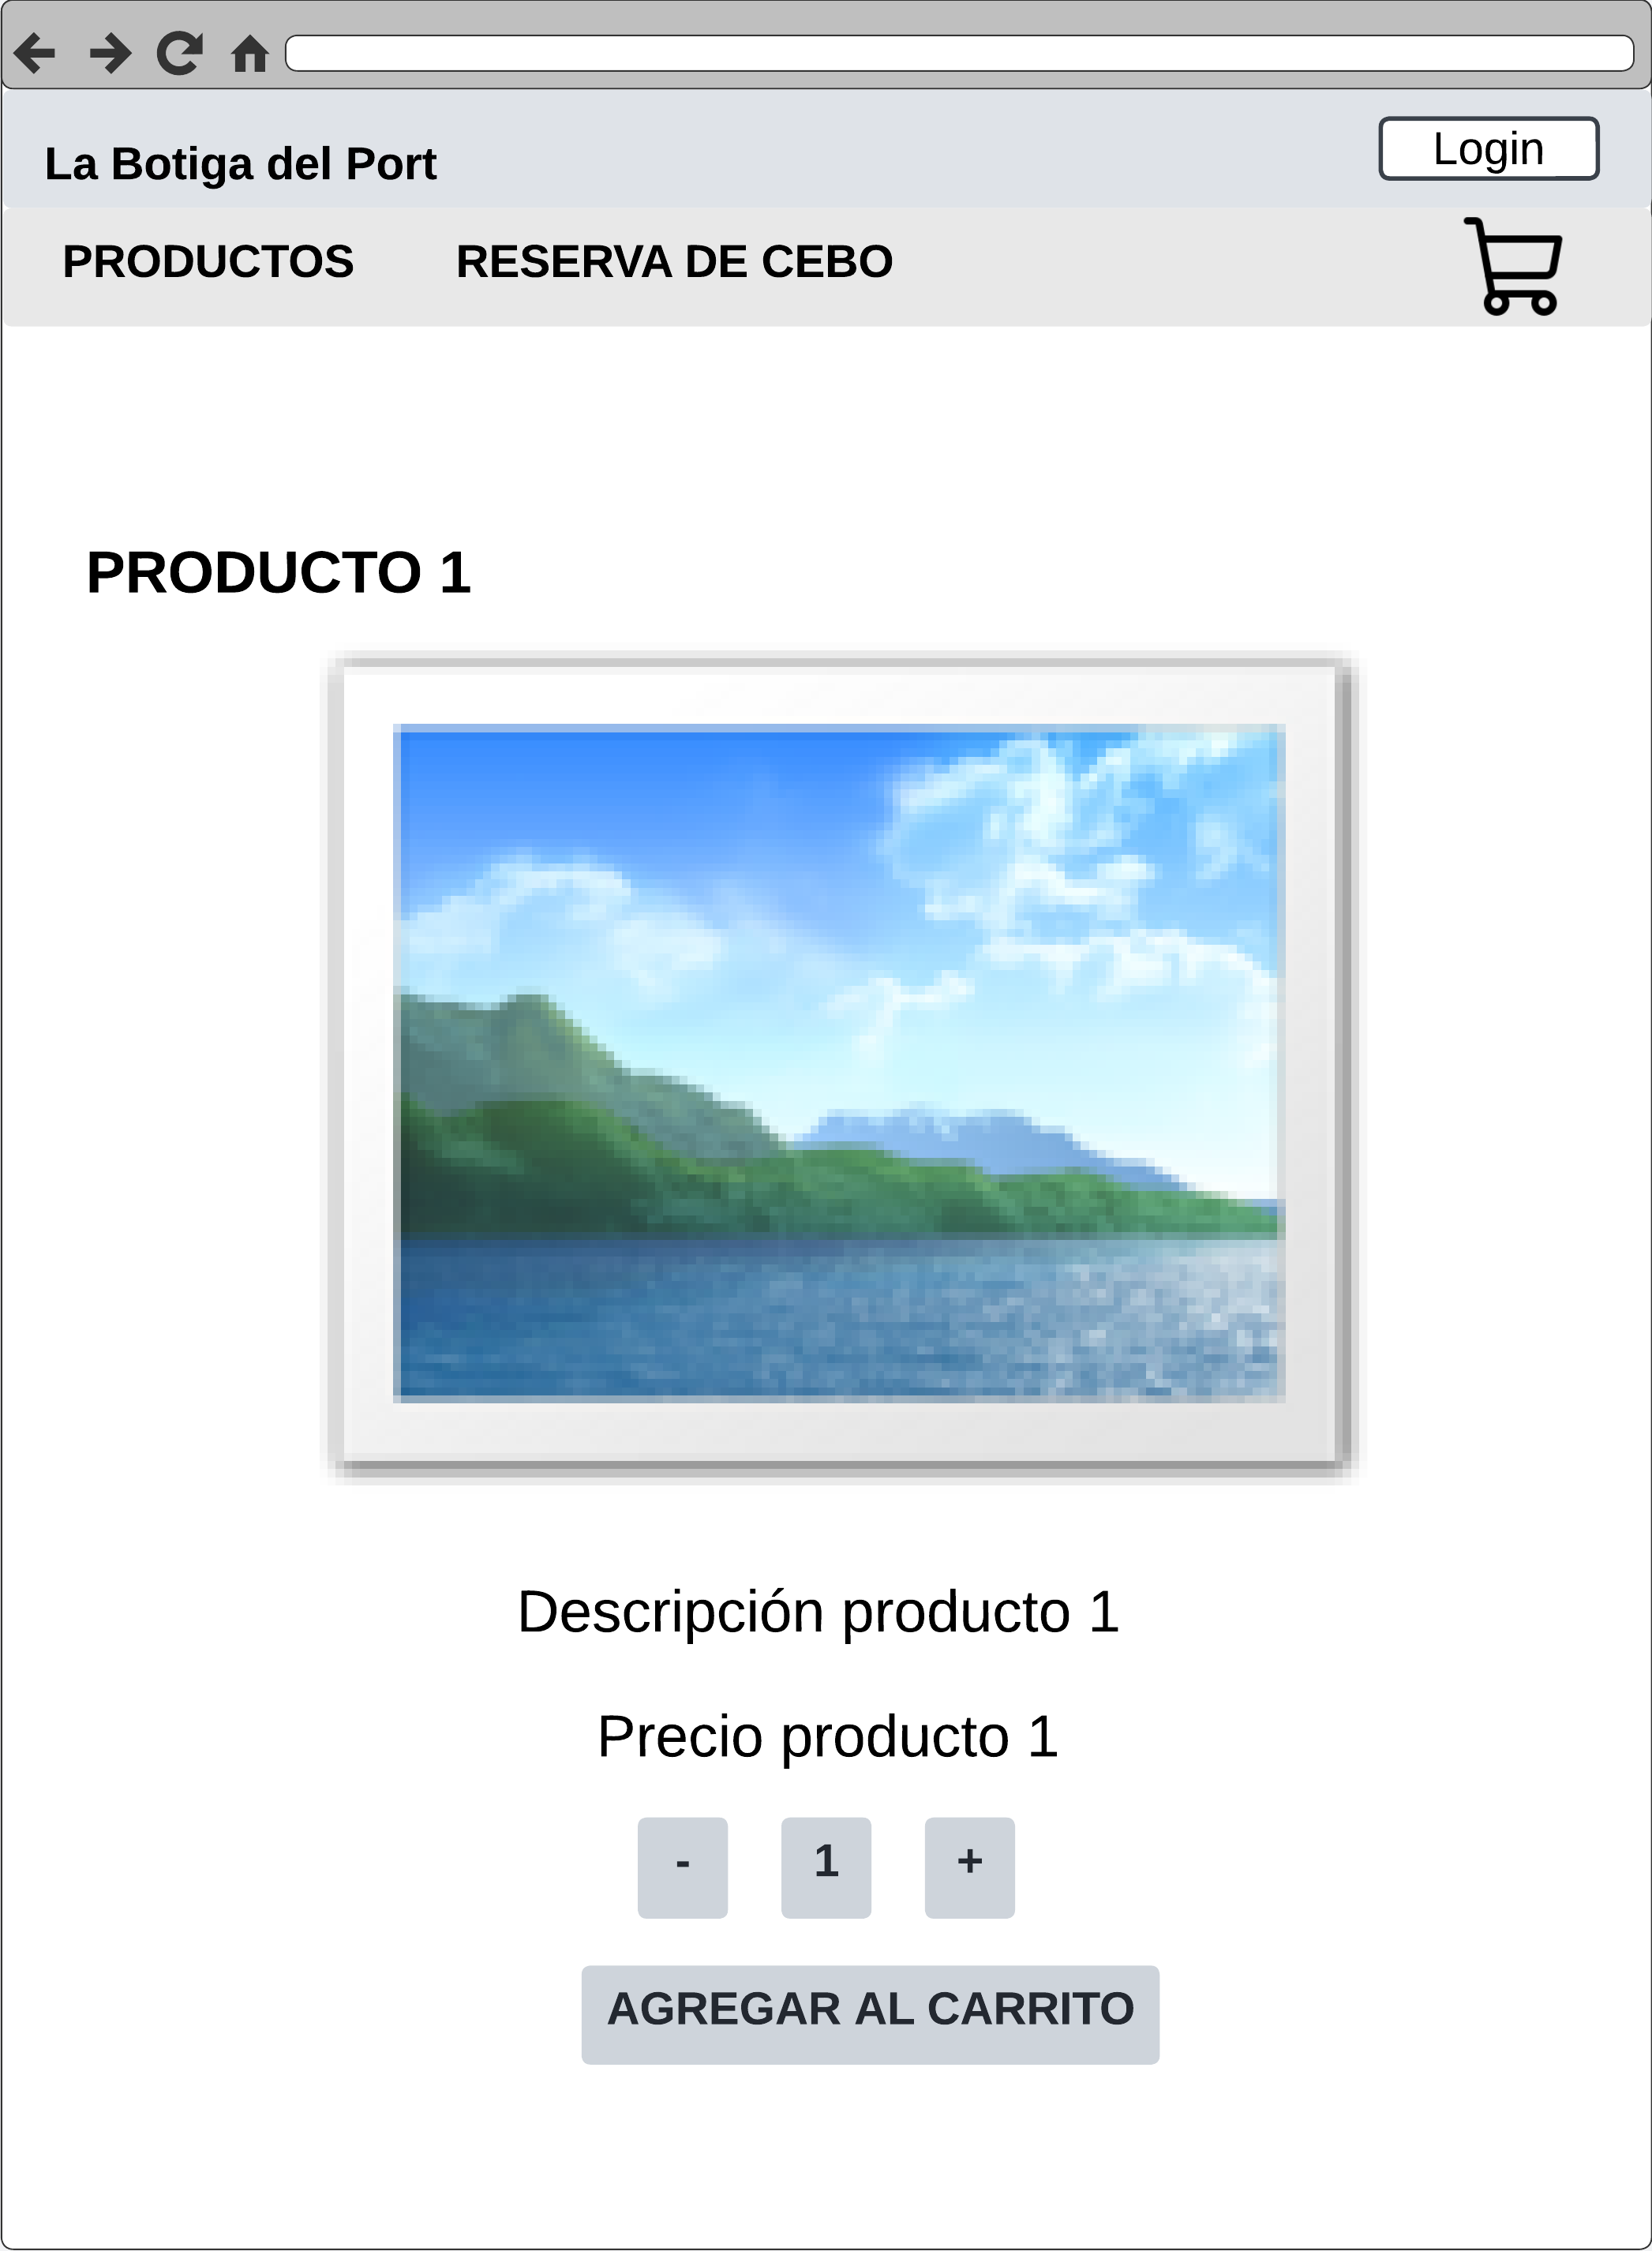
\includegraphics[scale=0.5]{./Images/detalle_producto.png}
\caption{Modelo de cliente - Página detalle del producto.} Fuente: Elaboración propia.

\label{fig:fig5}

\end{center}
\end{figure}

La Figura 4.6 muestra el resumen del pedido. Aquí, los usuarios pueden revisar y confirmar los productos seleccionados antes de finalizar su compra.


\begin{figure}[H]
\begin{center}
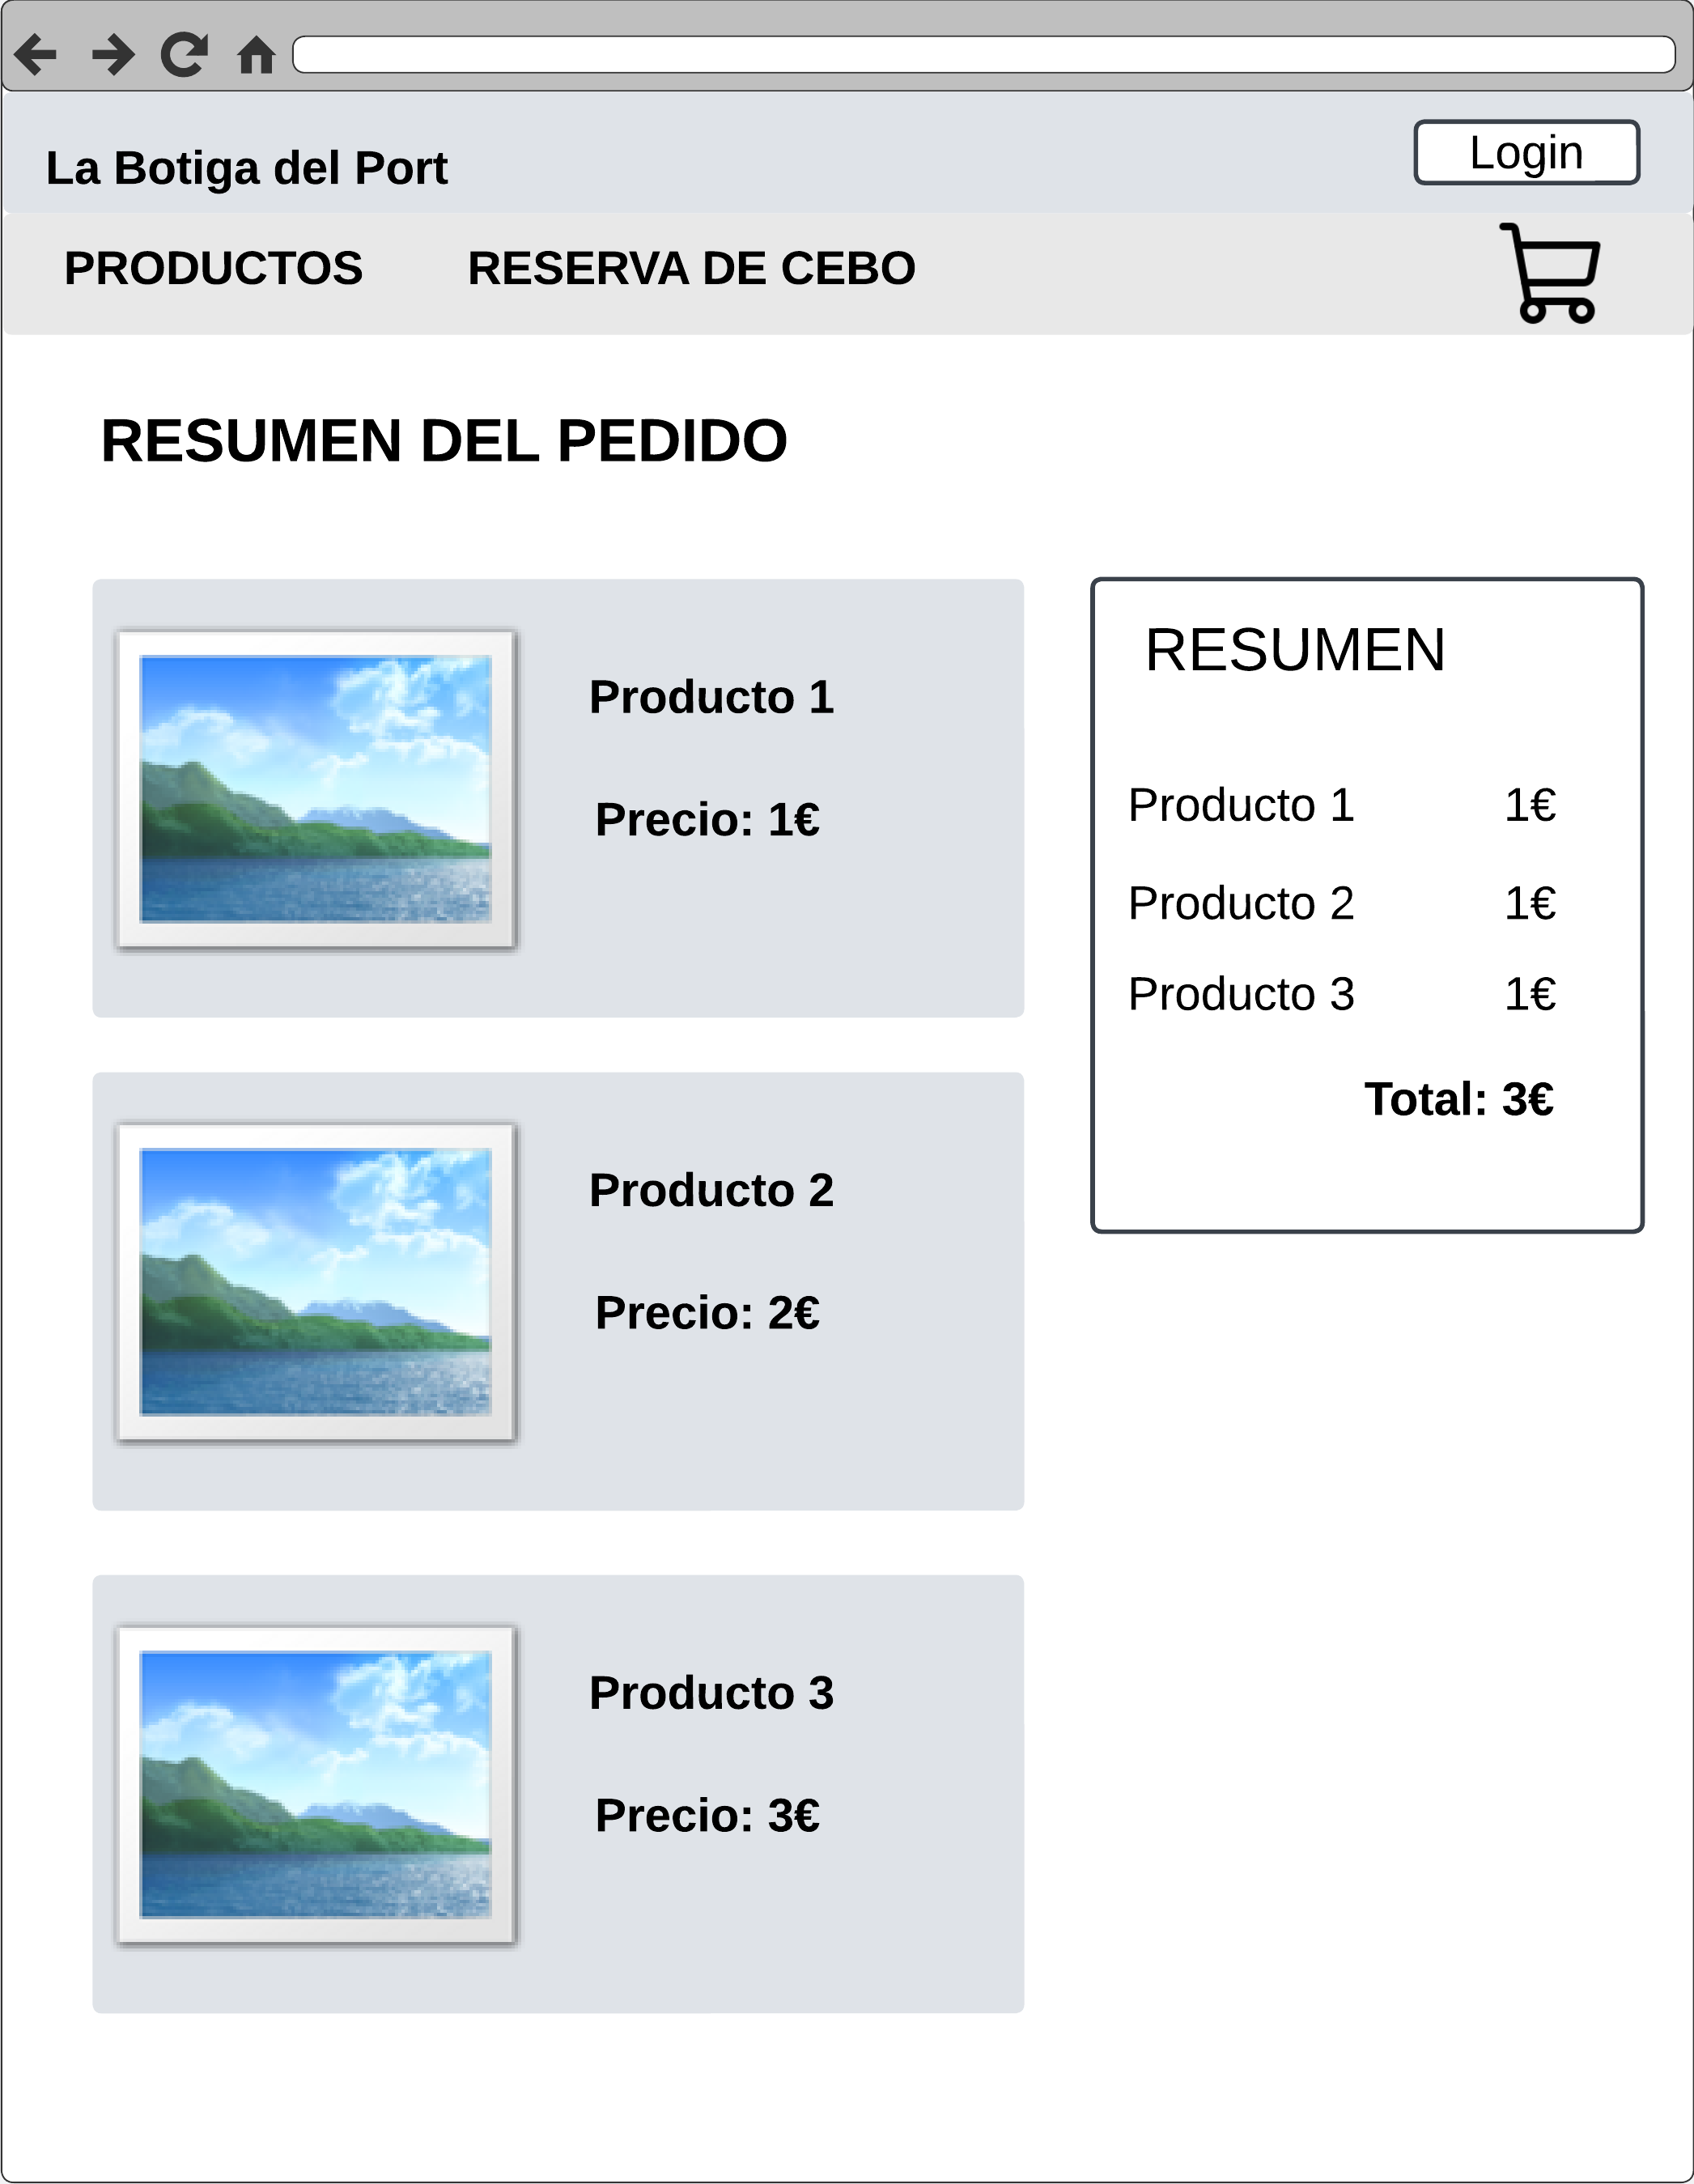
\includegraphics[scale=0.5]{./Images/pedido.png}
\caption{Modelo de cliente - Resumen del pedido.} Fuente: Elaboración propia.

\label{fig:fig6}

\end{center}
\end{figure}

En la Figura 4.7 se presenta la interfaz de reserva de cebo. Esta función permite a los usuarios reservar cebo disponible en la tienda para su compra posterior, asegurando que el cebo deseado esté reservado y disponible cuando el usuario lo necesite.


\begin{figure}[H]
\begin{center}
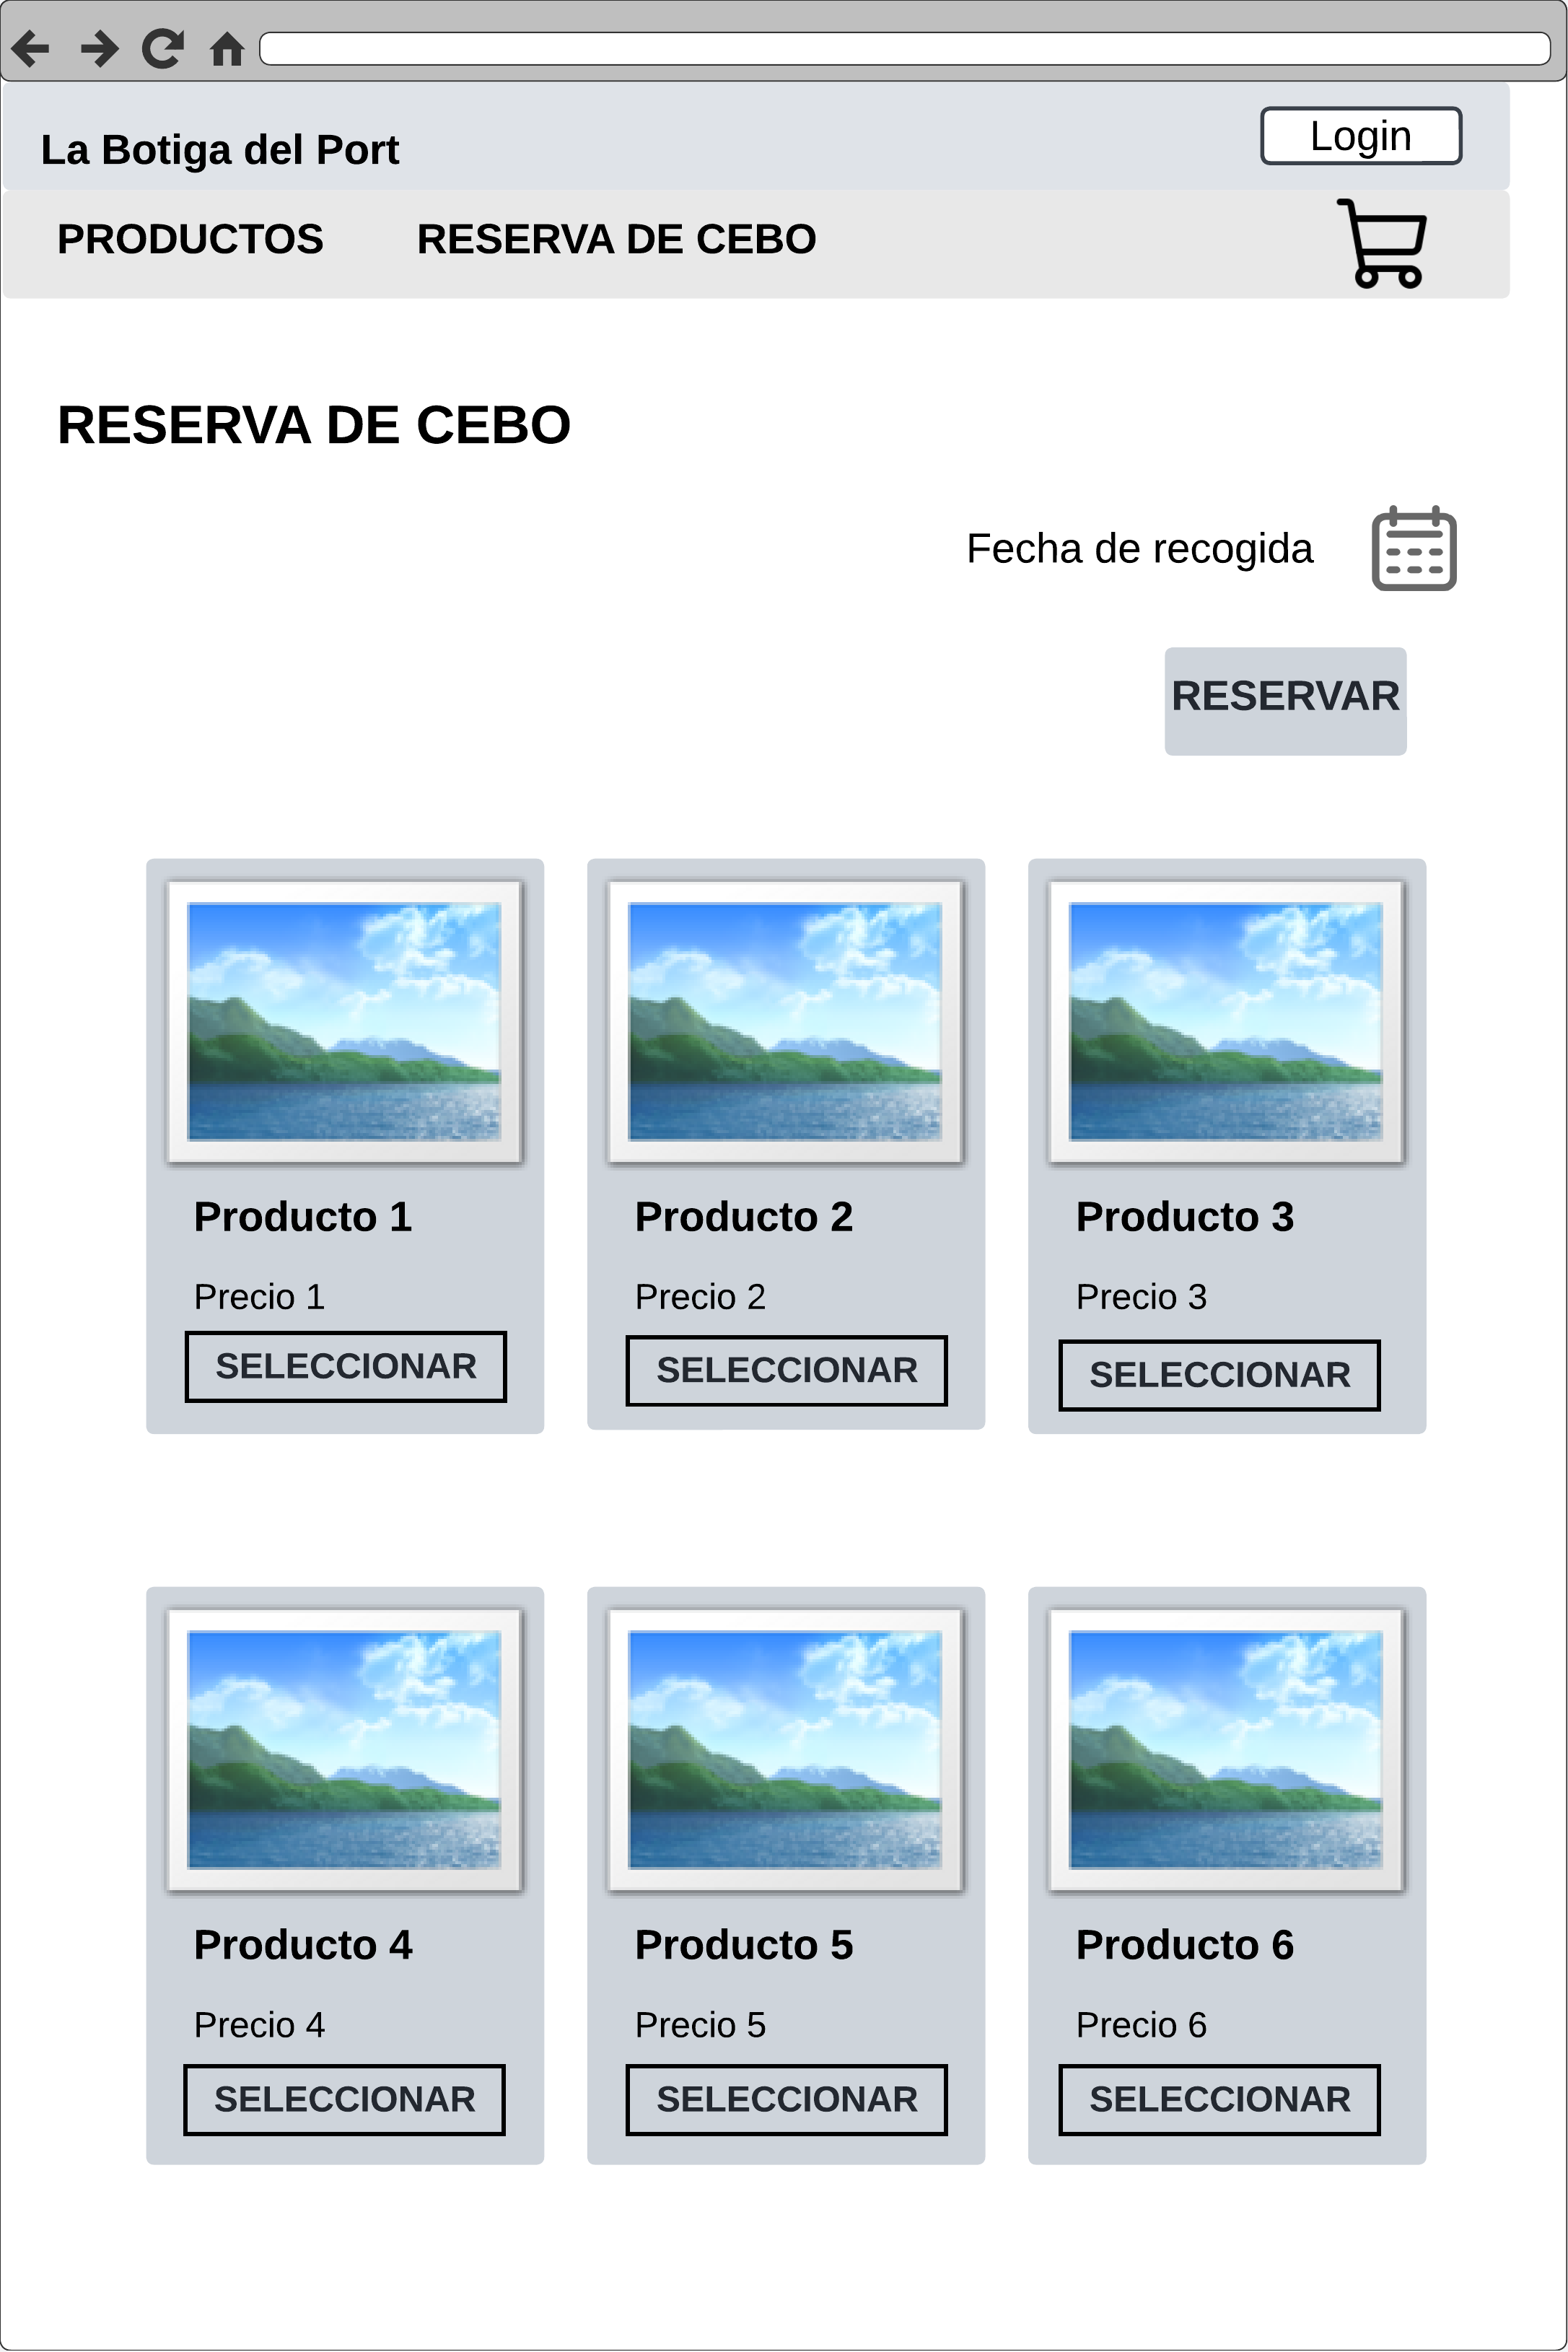
\includegraphics[scale=0.5]{./Images/reserva_cebo.png}
\caption{Modelo de cliente - Reserva de cebo.} Fuente: Elaboración propia.

\label{fig:fig7}

\end{center}
\end{figure}

\subsection{Mockup para el administrador}\label{subsec4.2.3}

En la Figura 4.8 se presenta el formulario de nuevo producto diseñado para el modo administrador. Esta interfaz permite al administrador agregar un nuevo producto al sistema proporcionando información detallada, como nombre, descripción, precio, cantidad e imágenes, facilitando la gestión eficiente del inventario.



\begin{figure}[H]
\begin{center}
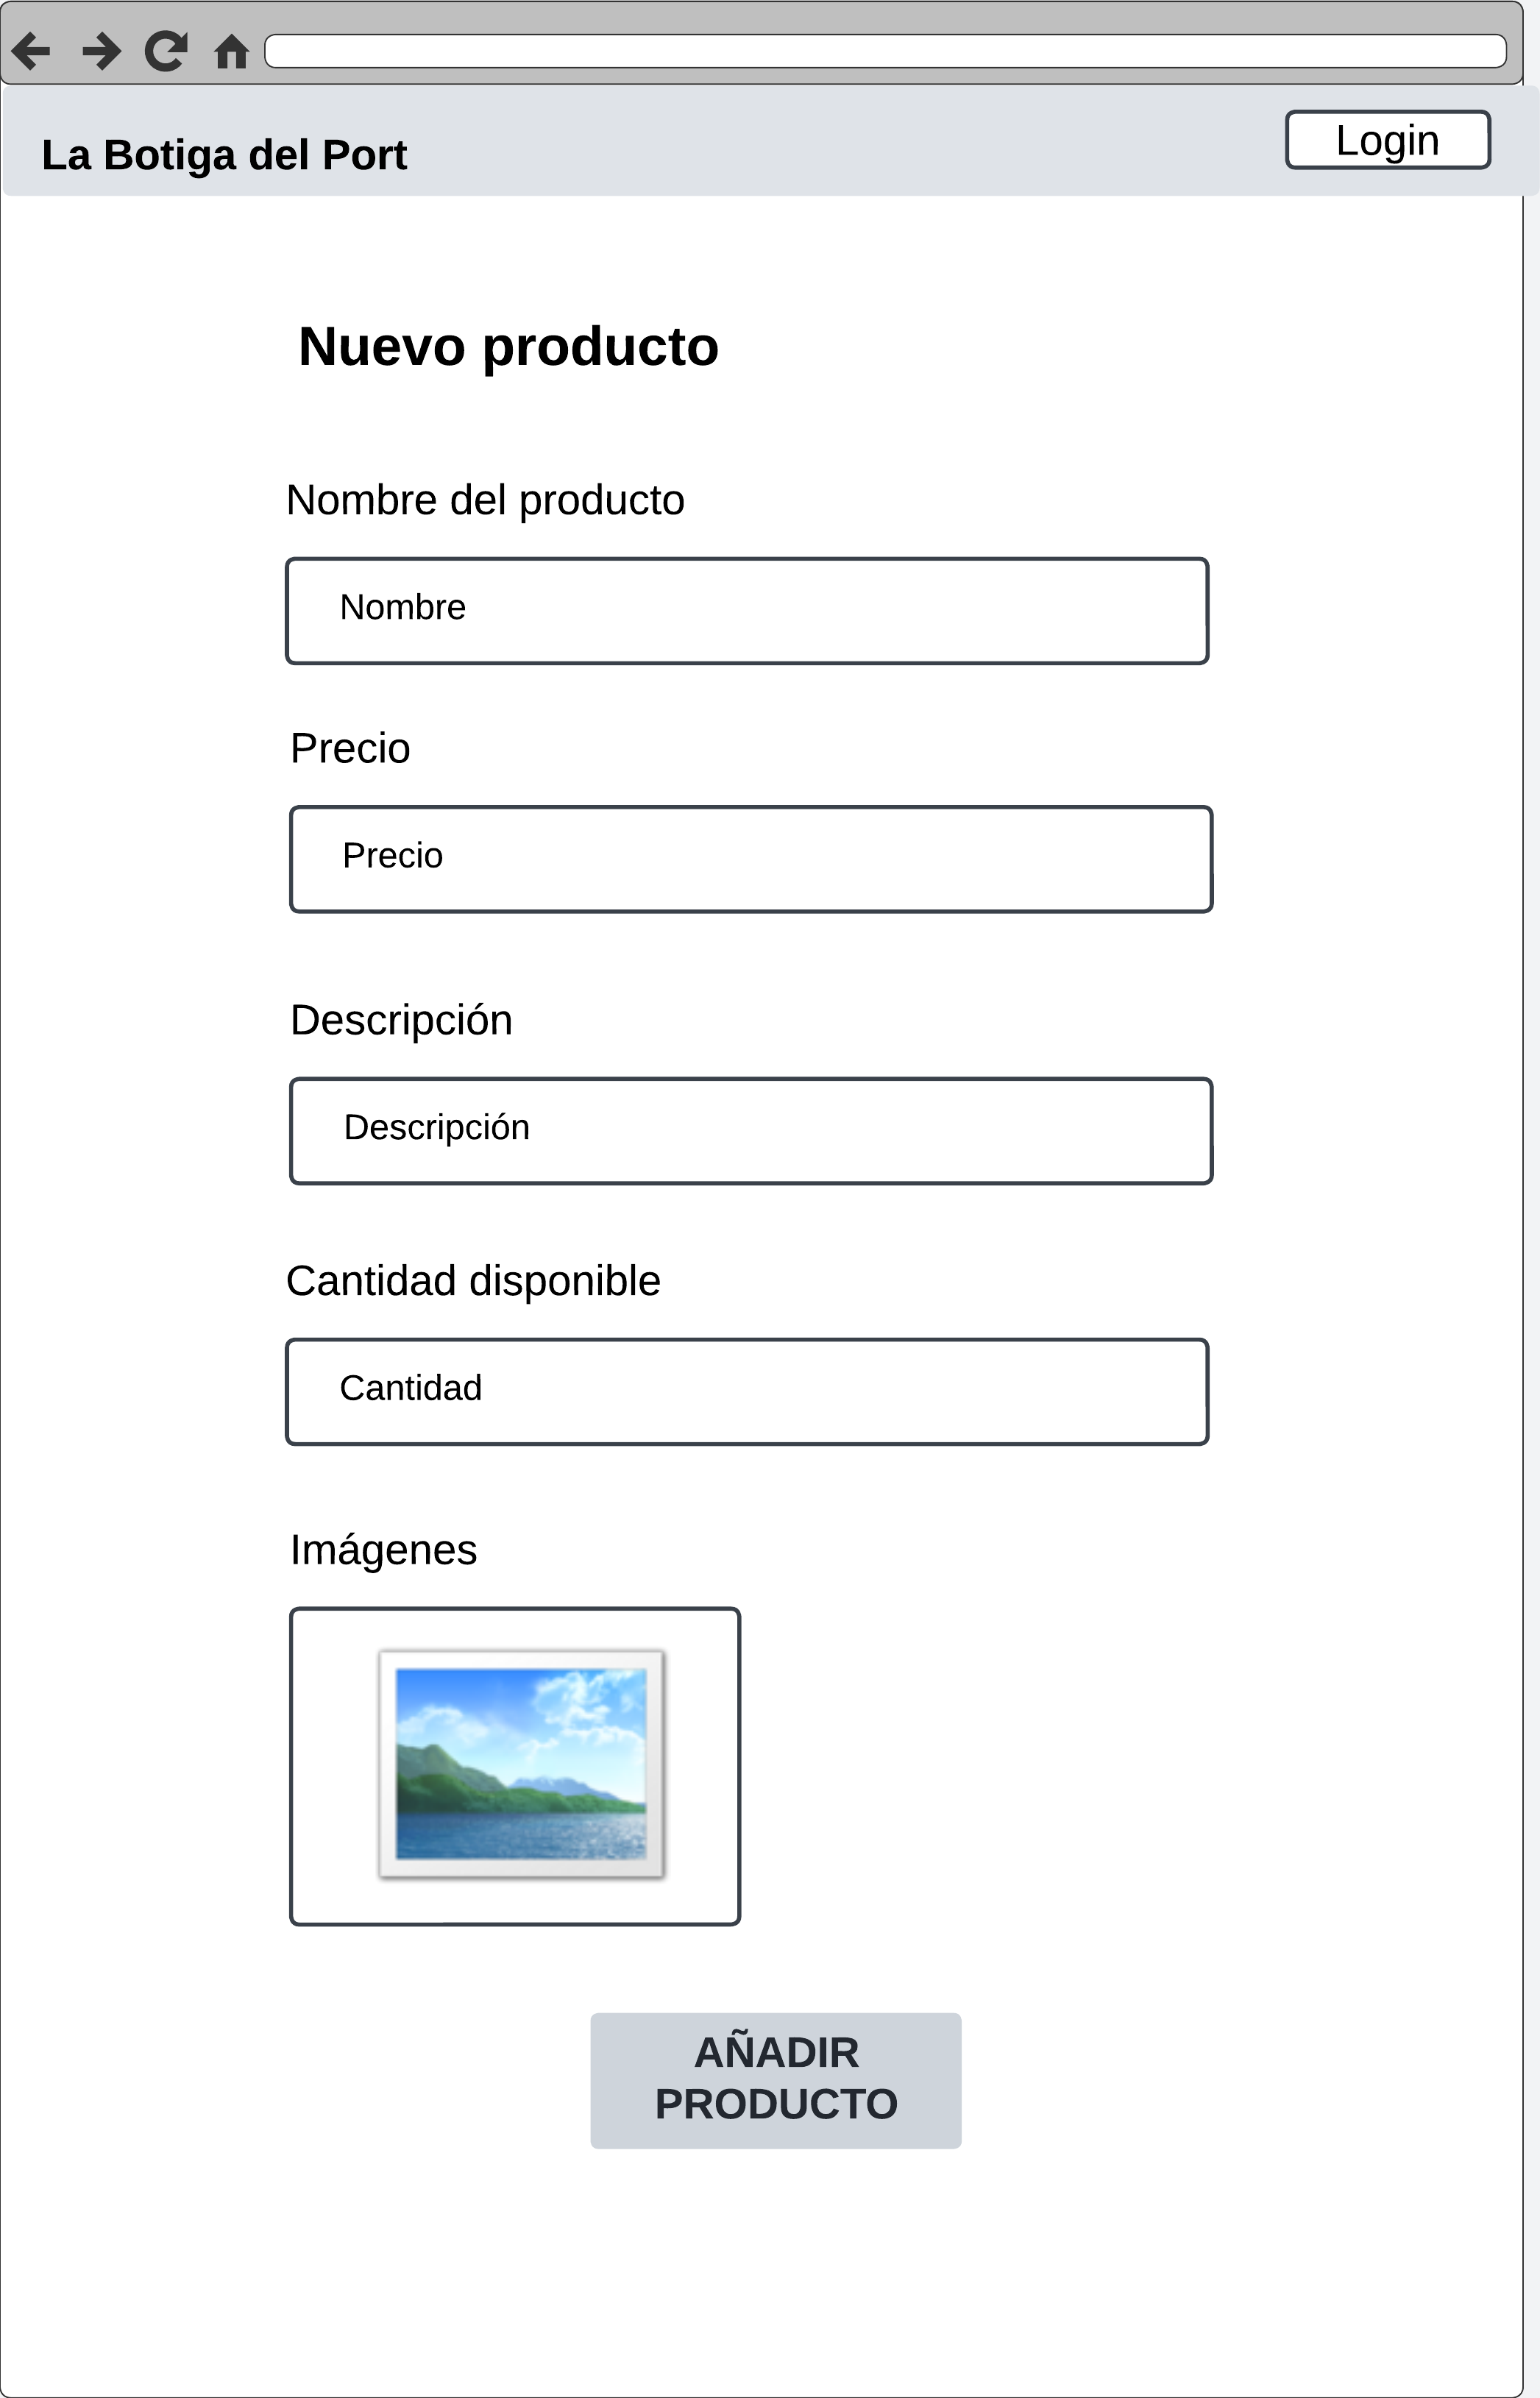
\includegraphics[scale=0.5]{./Images/nuevo_producto.png}
\caption{Modelo de administrador - Nuevo producto.} Fuente: Elaboración propia.

\label{fig:fig8}

\end{center}
\end{figure}

La Figura 4.9 muestra la vista de todos los productos existentes en el sistema. Esta interfaz proporciona al administrador una visión general de todos los productos almacenados, junto con opciones para editar o eliminar cada producto individualmente. 


\begin{figure}[H]
\begin{center}
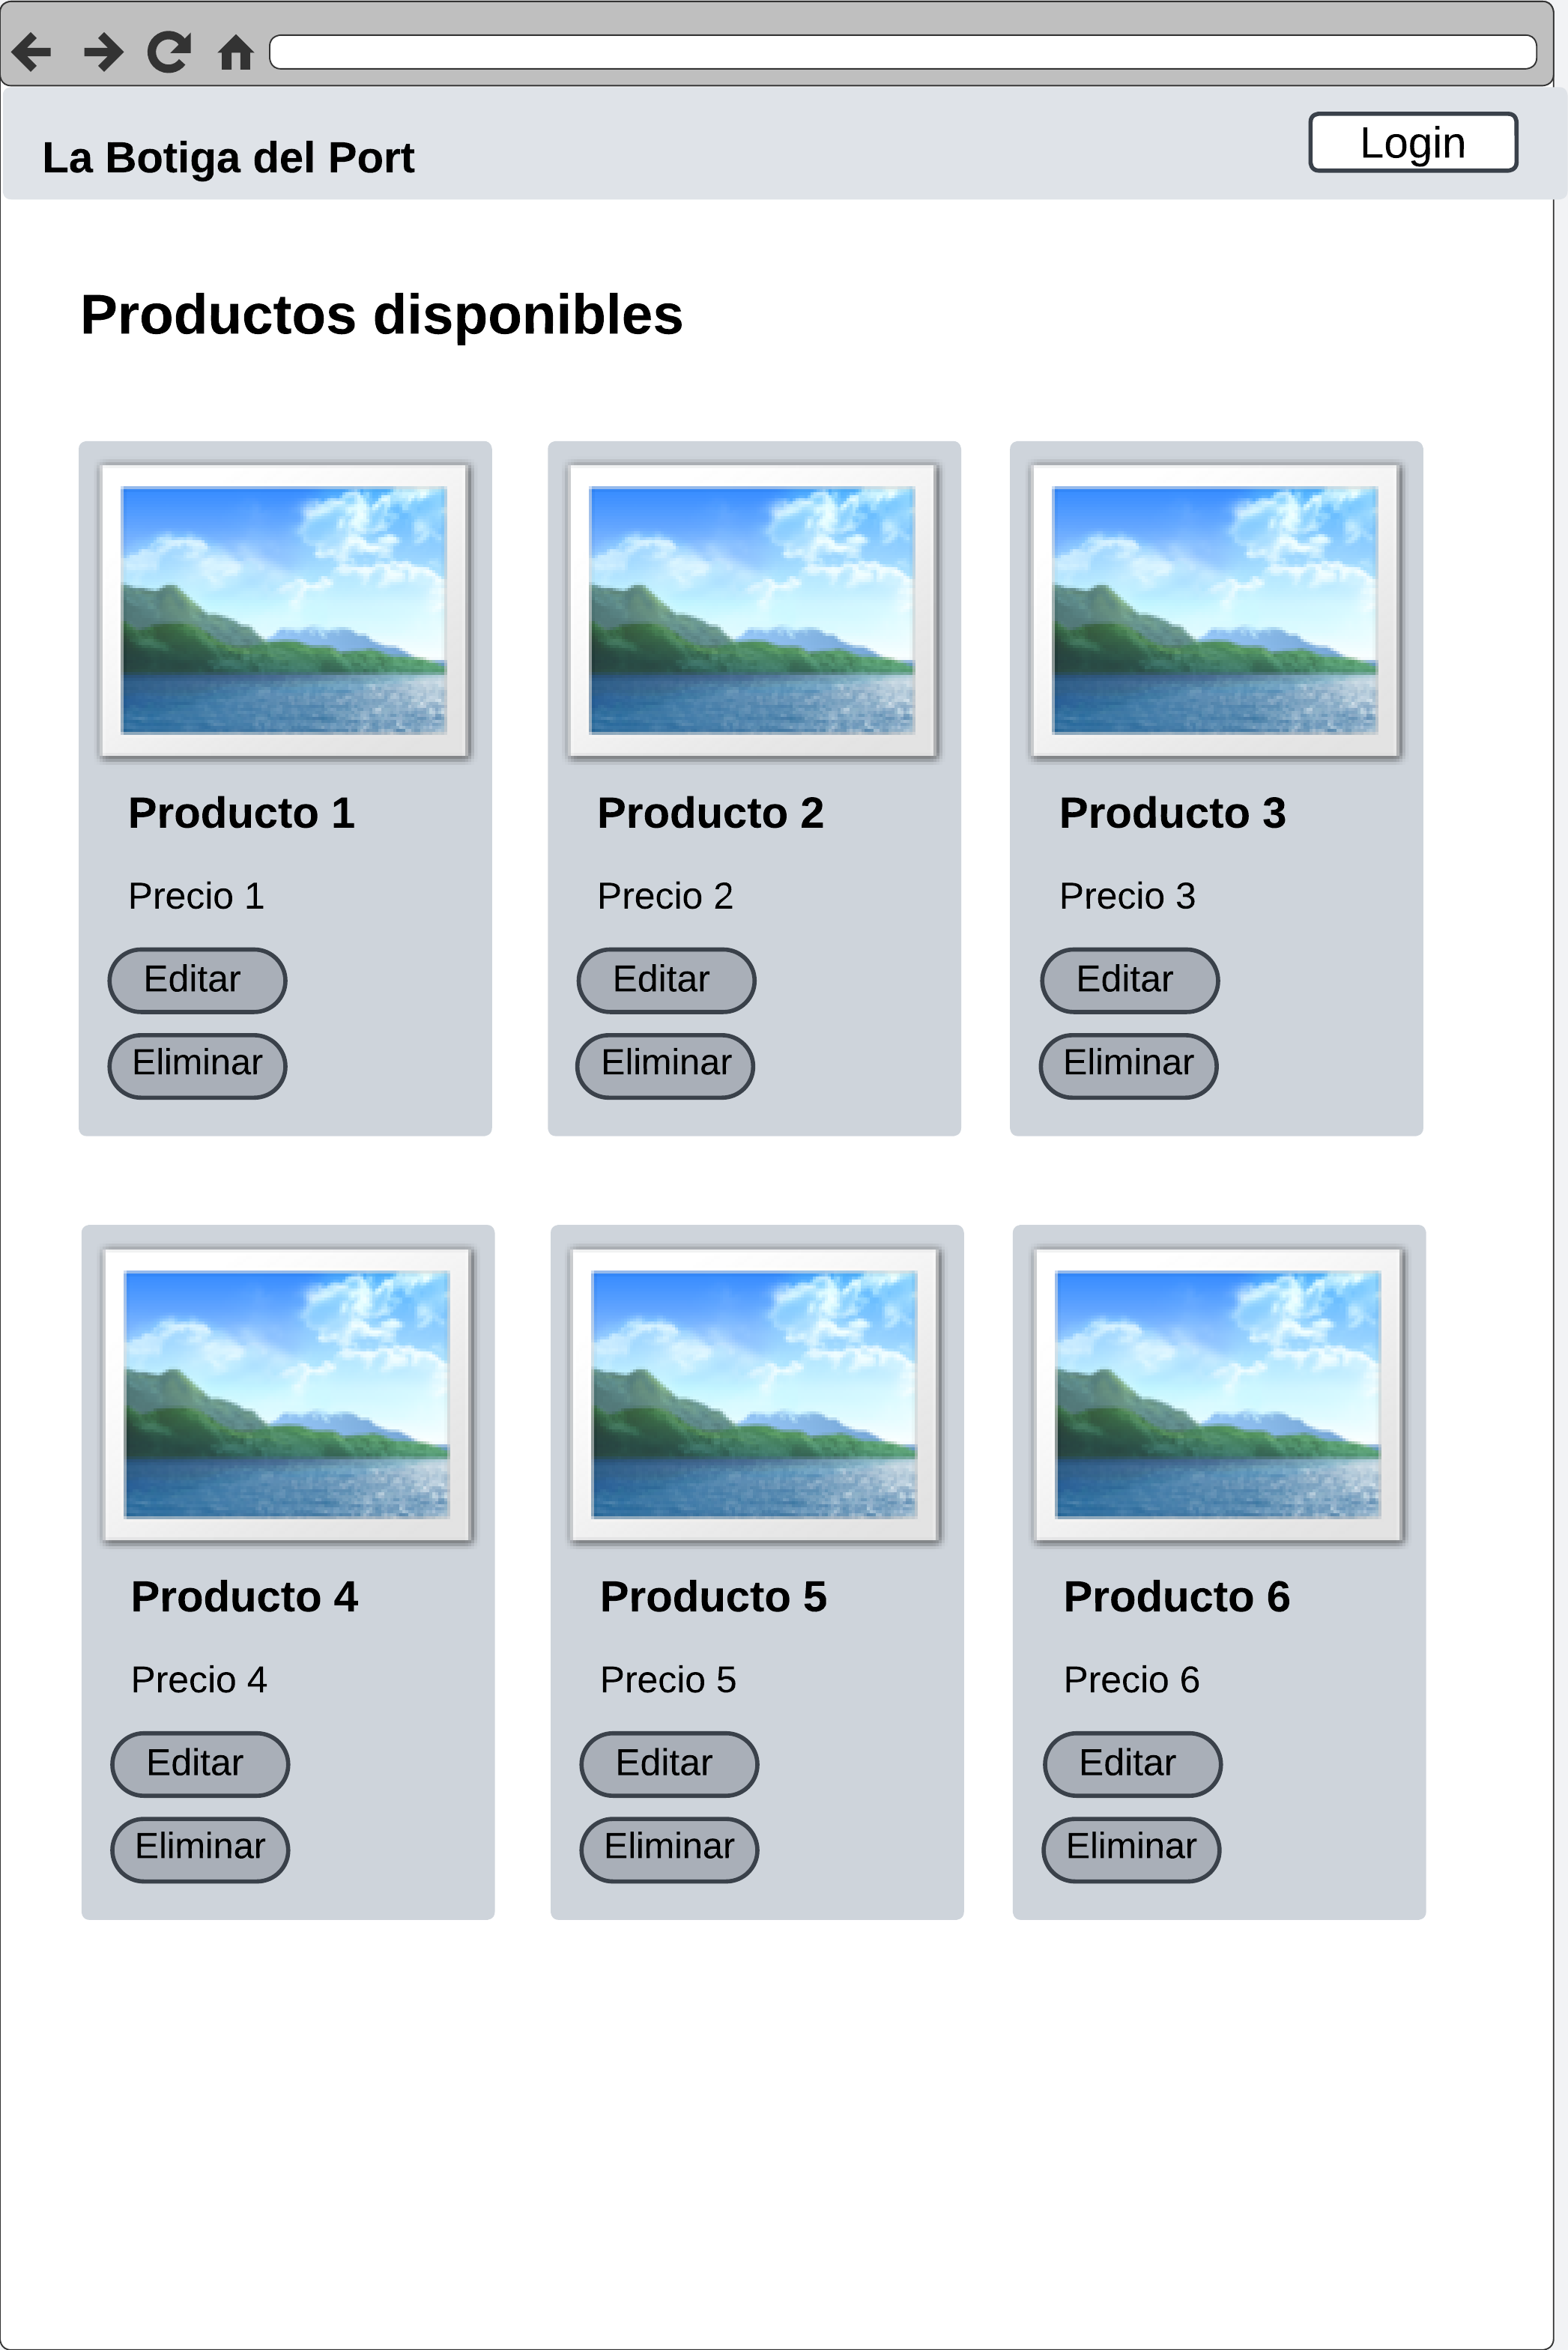
\includegraphics[scale=0.5]{./Images/productos_disponibles.png}
\caption{Modelo de administrador - Productos disponibles.} Fuente: Elaboración propia.

\label{fig:fig9}

\end{center}
\end{figure}

La Figura 4.10 muestra la vista de todas las reservas de cebo efectuadas. Esta interfaz proporciona al administrador una visión general de todas las reservas registradas, junto con opciones para marcarlas como recogidas o eliminarlas según sea necesario.

\begin{figure}[H]
\begin{center}
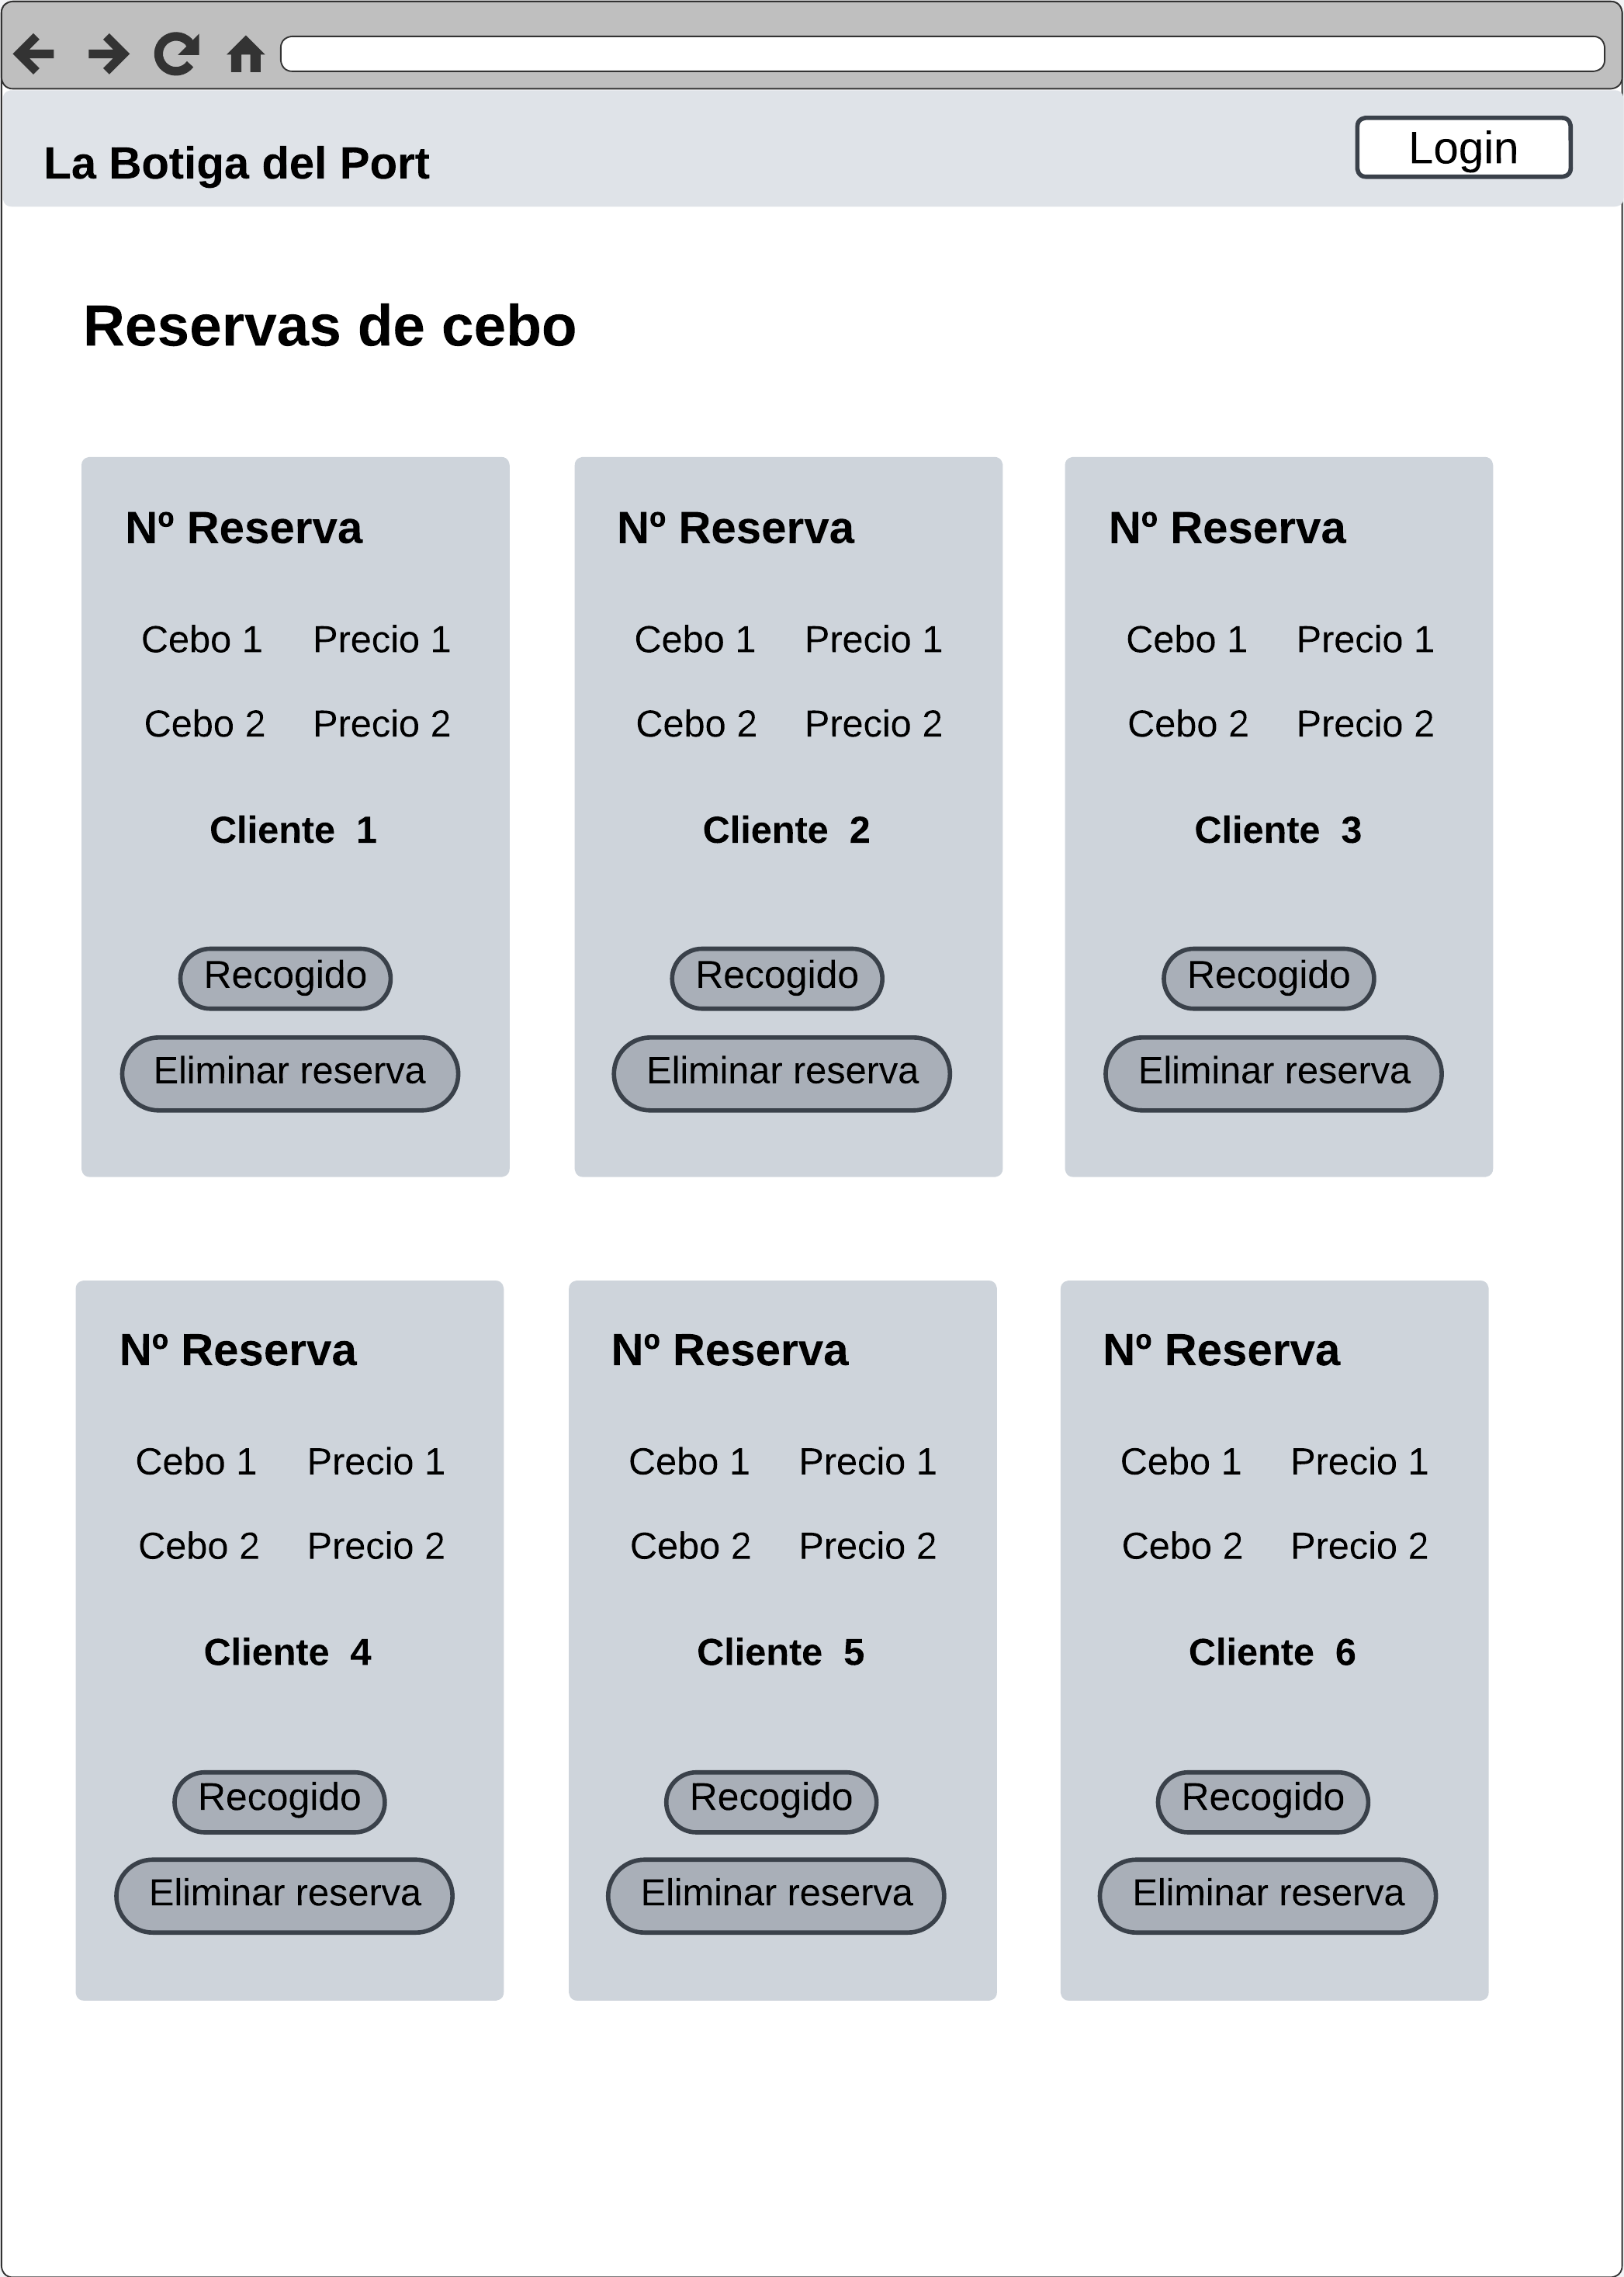
\includegraphics[scale=0.5]{./Images/reserva_cebo_admin.png}
\caption{Modelo de administrador - Reservas de cebo.} Fuente: Elaboración propia.

\label{fig:fig10}

\end{center}
\end{figure}

\section{Diseño BBDD - Diagrama ER}\label{sec:apartado}

La base de datos que sustenta la aplicación ha sido diseñada utilizando un enfoque relacional, con el objetivo de organizar y gestionar de manera eficiente la información generada. A partir de los requisitos específicos de la aplicación, se han identificado las entidades principales, sus atributos relevantes y las relaciones entre ellas. Cada entidad refleja un aspecto clave del sistema, como los productos, usuarios, pedidos y reservas de cebo, mientras que las relaciones aseguran la integridad y coherencia de los datos. Este proceso de modelado ha dado lugar a la creación del diagrama entidad-relación (ER), representado en la \textcolor{naranja}{Figura 4.11}, que proporciona una visión clara y estructurada de cómo se organiza la información en la base de datos y cómo interactúan los distintos elementos entre sí.

\begin{figure}[H]
\begin{center}
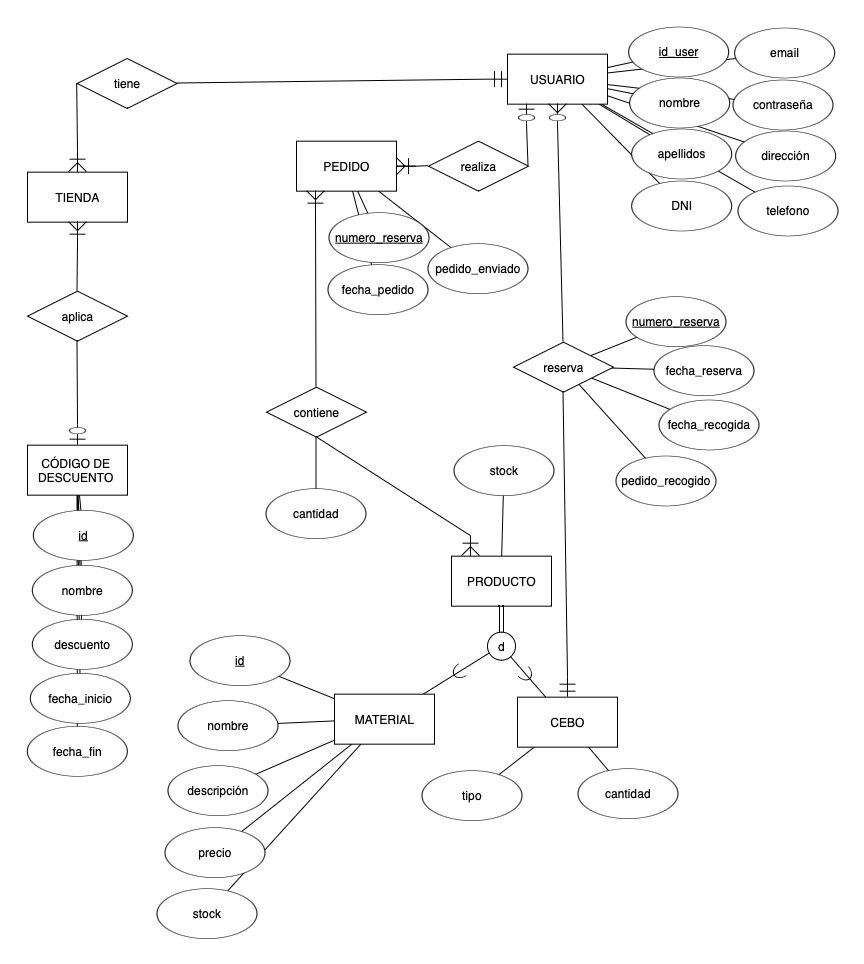
\includegraphics[scale=0.5]{./Images/diagramaER.png}
\caption{Diagrama ER.} Fuente: Elaboración propia.

\label{fig:fig11}

\end{center}
\end{figure}

El diagrama entidad-relación incluye las entidades relacionadas con los usuarios, la gestión de productos, las reservas de cebo y los pedidos, aspectos clave del funcionamiento de la aplicación. También se han incorporado las entidades necesarias para manejar códigos de descuento, los cuales podrán ser aplicados por los usuarios durante el proceso de compra.


\chapter{Resultados obtenidos}\label{cap:cap5}

A continuación, se detallarán los pasos realizados para el diseño y desarrollo de la aplicación, teniendo en cuenta los requisitos del proyecto y las historias de usuario definidas previamente. Se dividirá la explicación en varias secciones generales, cada una abordando un aspecto clave del proceso de desarrollo:


\begin{itemize}
    \item \textbf{Vistas de la aplicación.}
    
    \item \textbf{Uso de la aplicación.}
    
    \item \textbf{APIs utilizadas.}

    \item \textbf{Aspectos destacables de programación.}

    \item \textbf{Despliegue en entorno de producción.}

    \item \textbf{Costes del proyecto.}
    
\end{itemize}


Cada una de estas secciones será tratada en profundidad en las siguientes subsecciones, proporcionando un análisis detallado de la información correspondiente a cada tema.

\section{Vistas de la aplicación}\label{sec:apartado}

Los modelos de las vistas de la \textcolor{naranja}{sección 4.2 - Modelos para la interfaz - Mockup}
 funcionan como una referencia tanto para el desarrollador como para el cliente, permitiendo una primera aproximación visual de lo que será la aplicación. 

\vspace{0.5cm}

A continuación, se presentan las vistas finales de la aplicación, que han sufrido pocas modificaciones respecto a los modelos iniciales. Además, se describirán de manera general las funcionalidades principales de estas vistas, mientras que el detalle completo se abordará en la  \textcolor{naranja}{sección 5.2 - Uso de la aplicación}.

\vspace{0.5cm}
Procederemos a diferenciar las vistas en cuatro secciones: las destinadas al cliente, las correspondientes al administrador, la vista de la ubicación y la vista responsive, que muestra cómo se adapta la interfaz en dispositivos móviles.

\subsection{Vista para el cliente}\label{subsec5.1.1}

\subsubsection{Login y registro}\label{subsec5.1.1.1}


La vista de login está diseñada para proporcionar una interfaz simple y clara donde los usuarios pueden introducir sus credenciales (correo electrónico y contraseña) para acceder a su cuenta. La estructura visual de esta vista es minimalista, destacando el formulario de autenticación en el centro de la página. Se incluyen campos de texto para el correo electrónico y la contraseña, esta última oculta por defecto para garantizar la seguridad, aunque los usuarios pueden optar por mostrarla utilizando un botón específico. Junto a estos campos, se encuentran botones claramente etiquetados para iniciar sesión (login) y registrarse en caso de no tener cuenta. La vista también ofrece mensajes de error en caso de que los intentos de autenticación sean fallidos.

\begin{figure}[H]
\begin{center}
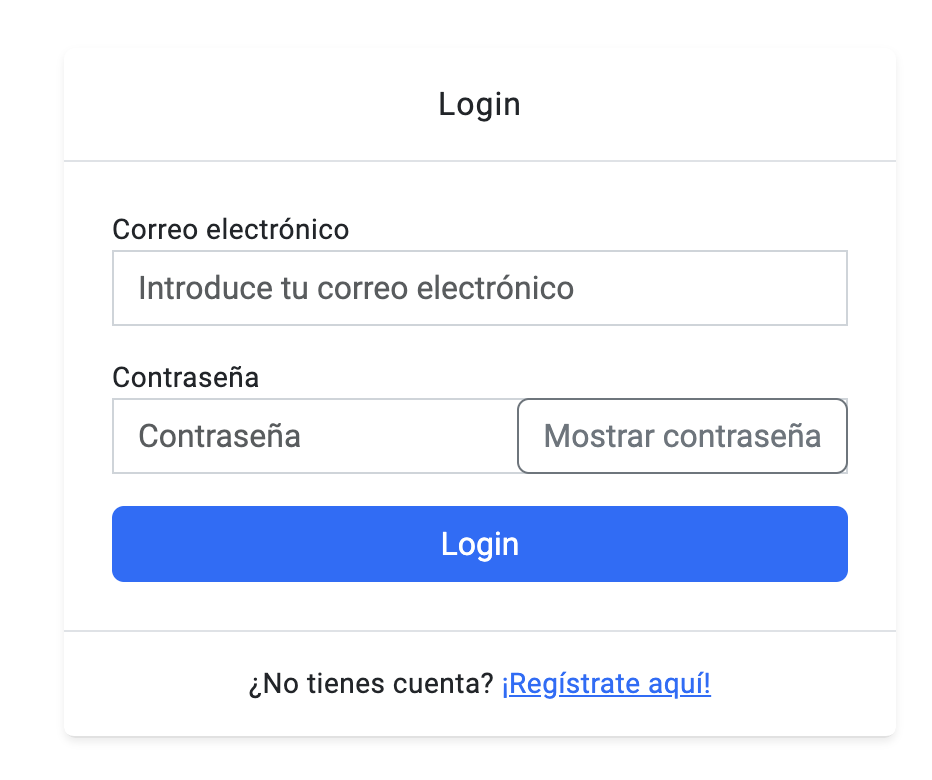
\includegraphics[scale=0.5]{./Images/vista_login.png}
\caption{Vista login} Fuente: Elaboración propia.

\label{fig:fig1}

\end{center}
\end{figure}

La vista de registro presenta un formulario que permite a los nuevos usuarios crear una cuenta en la plataforma. Esta vista está diseñada para ser intuitiva, con campos claramente etiquetados que guían al usuario a través del proceso de registro. Los campos incluyen información básica como nombre y apellidos, identificación, dirección de correo electrónico, y contraseña, además de campos para la dirección. El diseño prioriza la usabilidad y la seguridad, con elementos visuales que validan la información en tiempo real y aseguran que el proceso de registro sea lo más fluido posible.

\begin{figure}[H]
\begin{center}
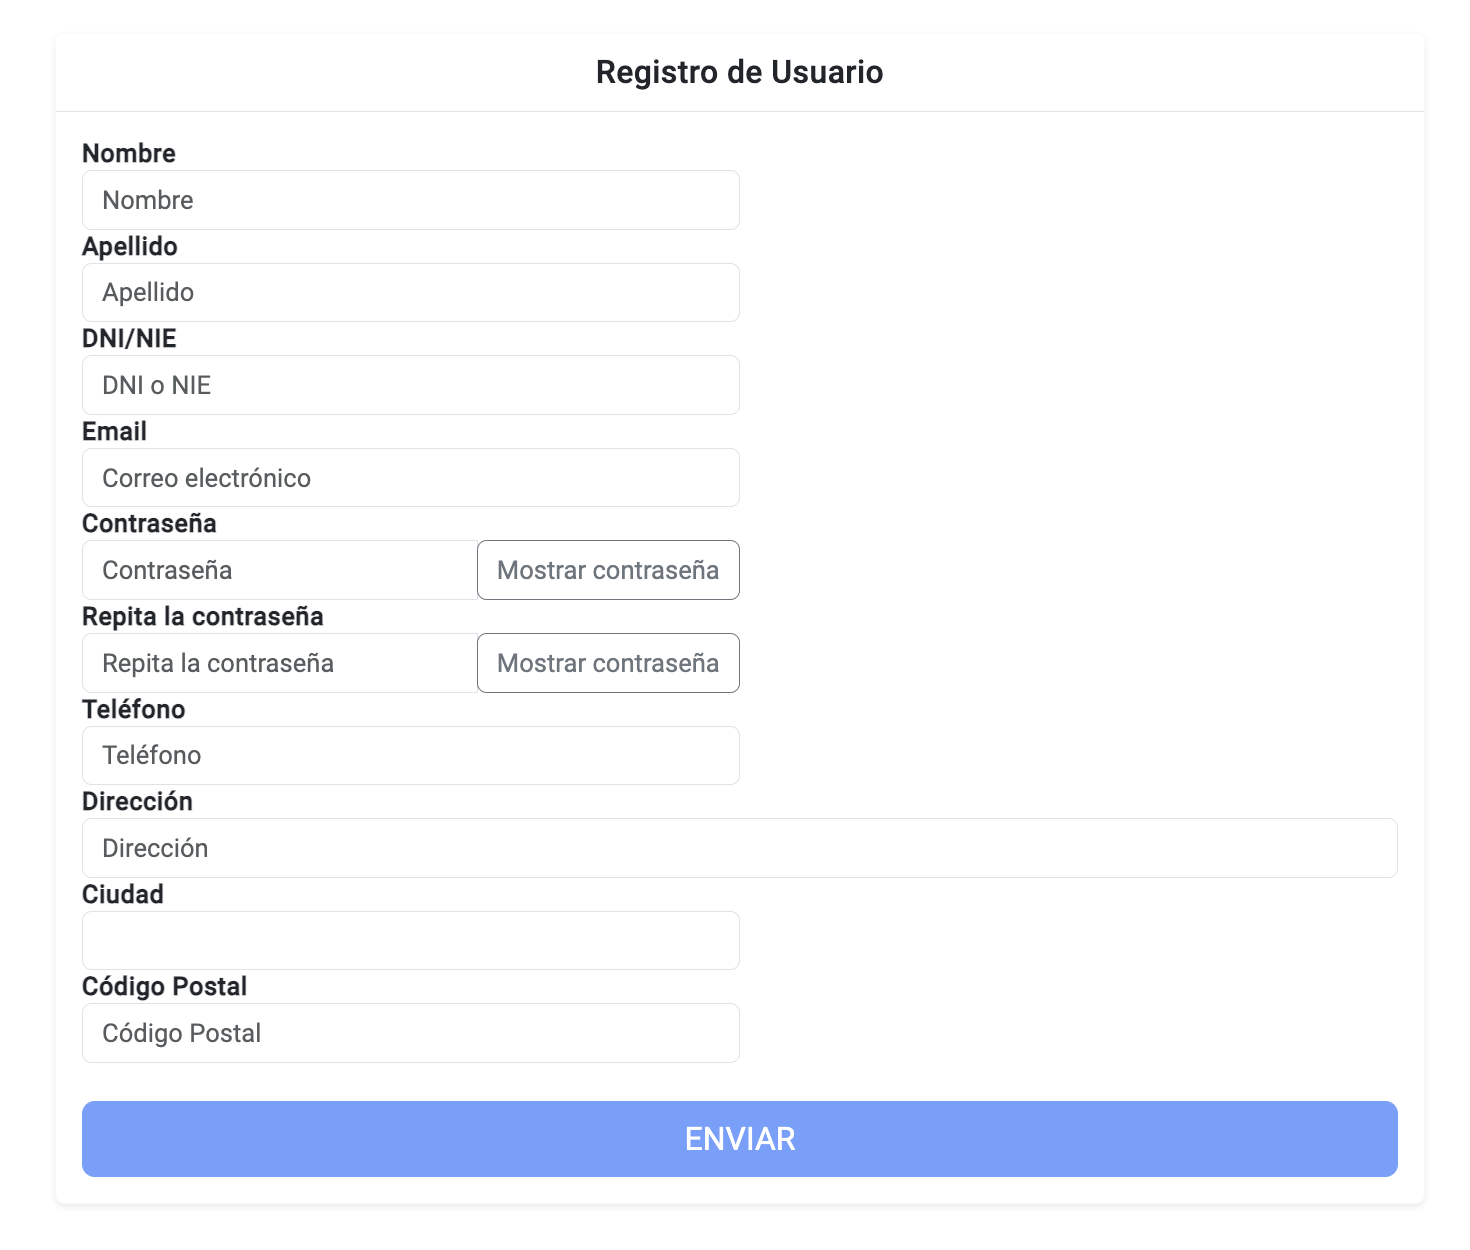
\includegraphics[scale=0.5]{./Images/vista_registro.png}
\caption{Vista registro de usuario} Fuente: Elaboración propia.

\label{fig:fig2}

\end{center}
\end{figure}

\subsubsection{Productos y pedidos}\label{subsec5.1.1.2}

En la vista de productos, se muestran todos los artículos dentro de la categoría seleccionada. Cada producto se presenta con su imagen, nombre, subcategoría, y precio. Además, se incluye una etiqueta informativa que indica si el producto está en oferta, agotado o si forma parte de las últimas novedades

\begin{figure}[H]
\begin{center}
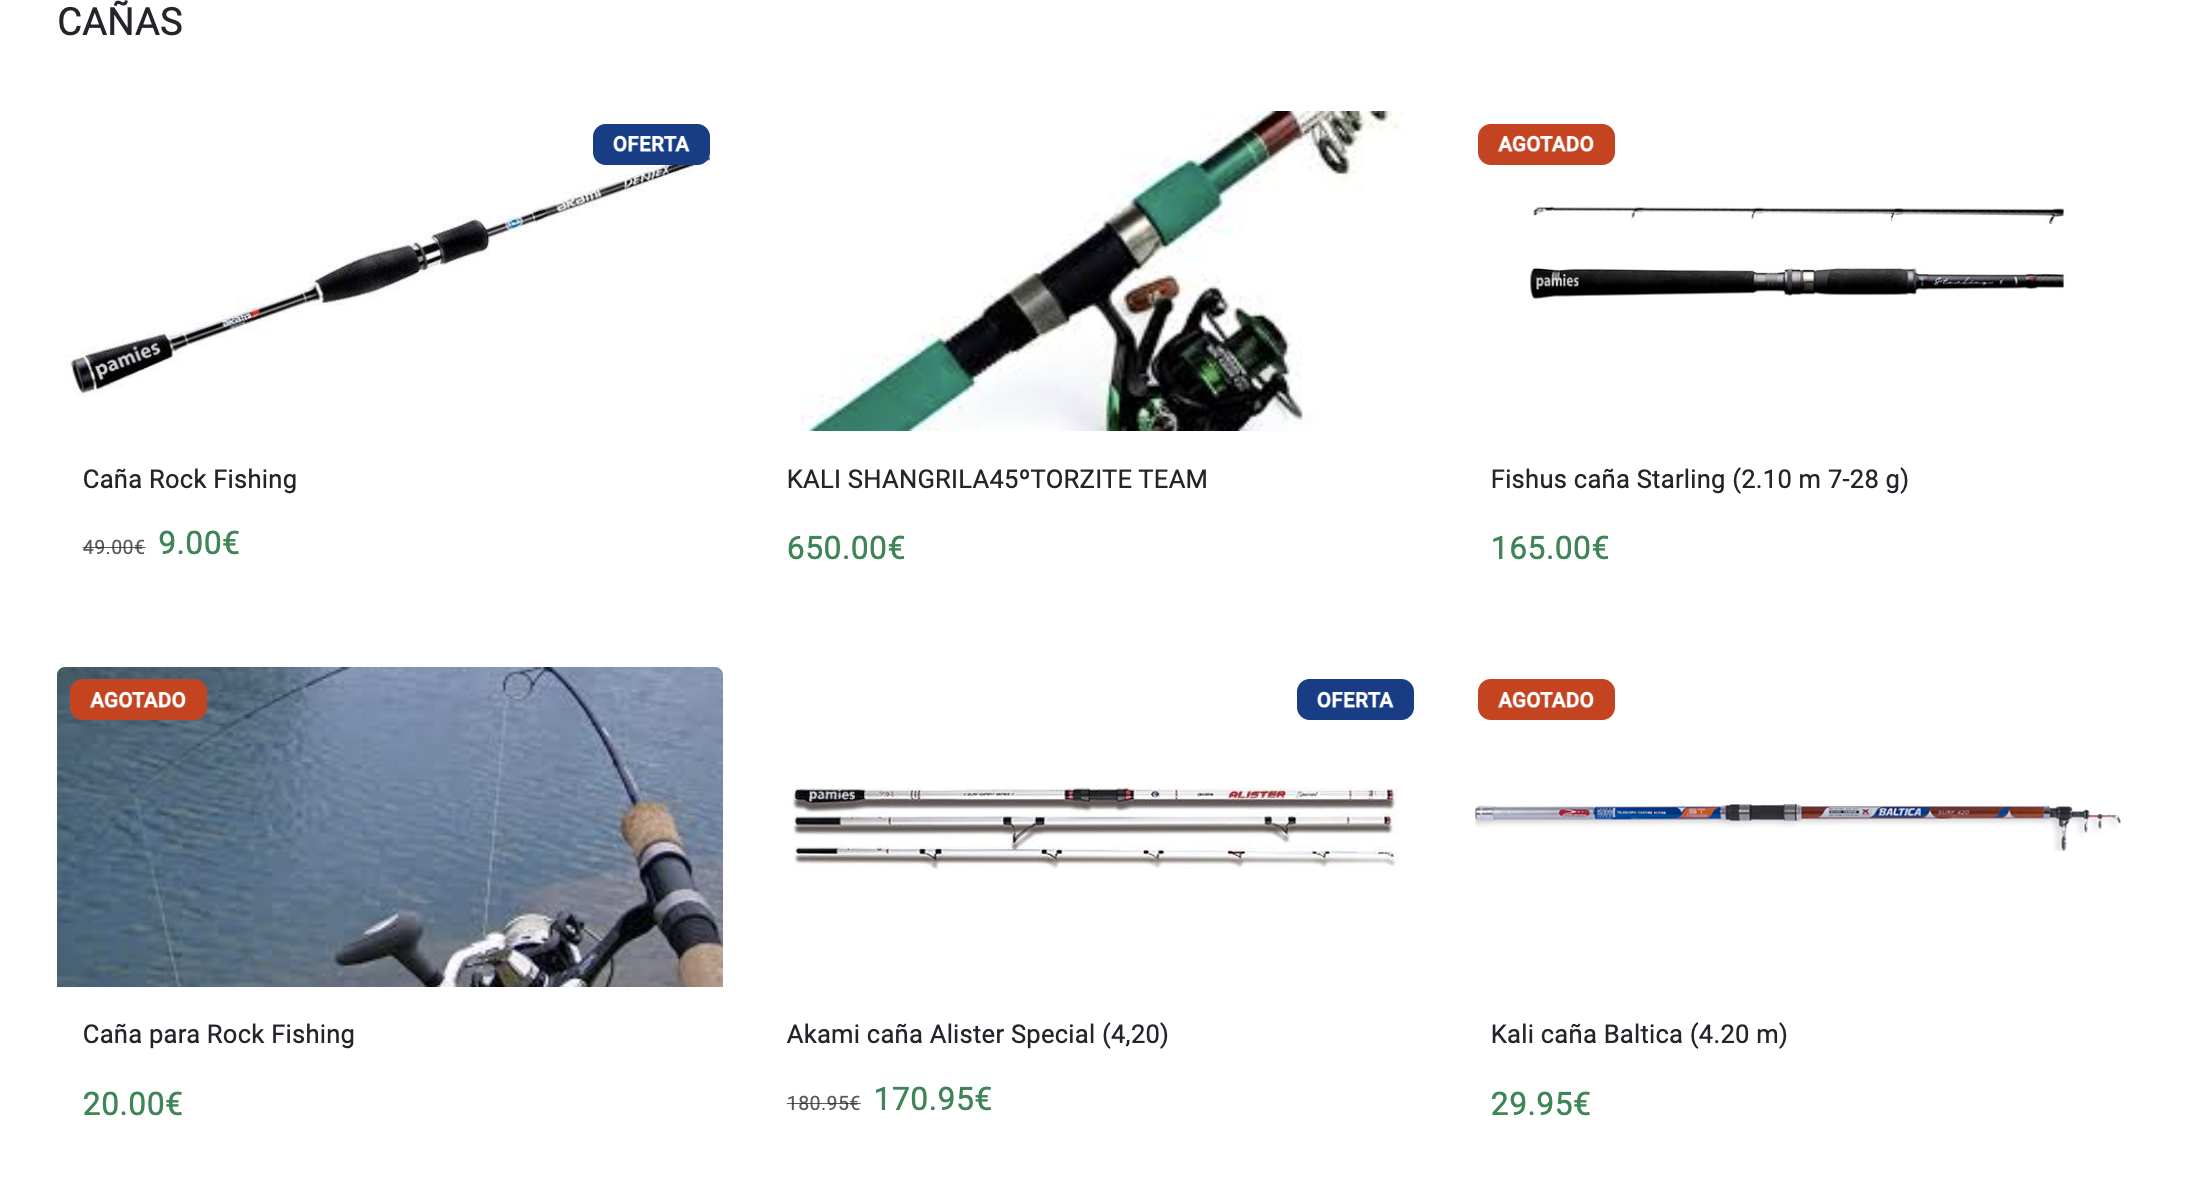
\includegraphics[scale=0.40]{./Images/vistaProductos.png}
\caption{Vista Productos} Fuente: Elaboración propia.

\label{fig:fig2}

\end{center}
\end{figure}


La aplicación también ofrece una vista detallada para cada producto, accesible desde la lista de productos clasificados. En esta vista, los usuarios pueden ver una descripción completa del producto, que incluye información detallada sobre sus características y especificaciones. Además, se muestran múltiples imágenes del producto desde diferentes ángulos, lo que permite a los usuarios examinarlo con mayor precisión. El precio del producto está claramente indicado junto a un botón destacado que permite añadirlo al carrito de compras. También se incluye un campo donde los usuarios pueden especificar la cantidad deseada del producto antes de añadirlo al carrito. Esta vista está diseñada para proporcionar toda la información necesaria para que los usuarios puedan tomar decisiones de compra informadas, al tiempo que facilita el proceso de añadir productos al carrito en las cantidades deseadas.


\begin{figure}[H]
\begin{center}
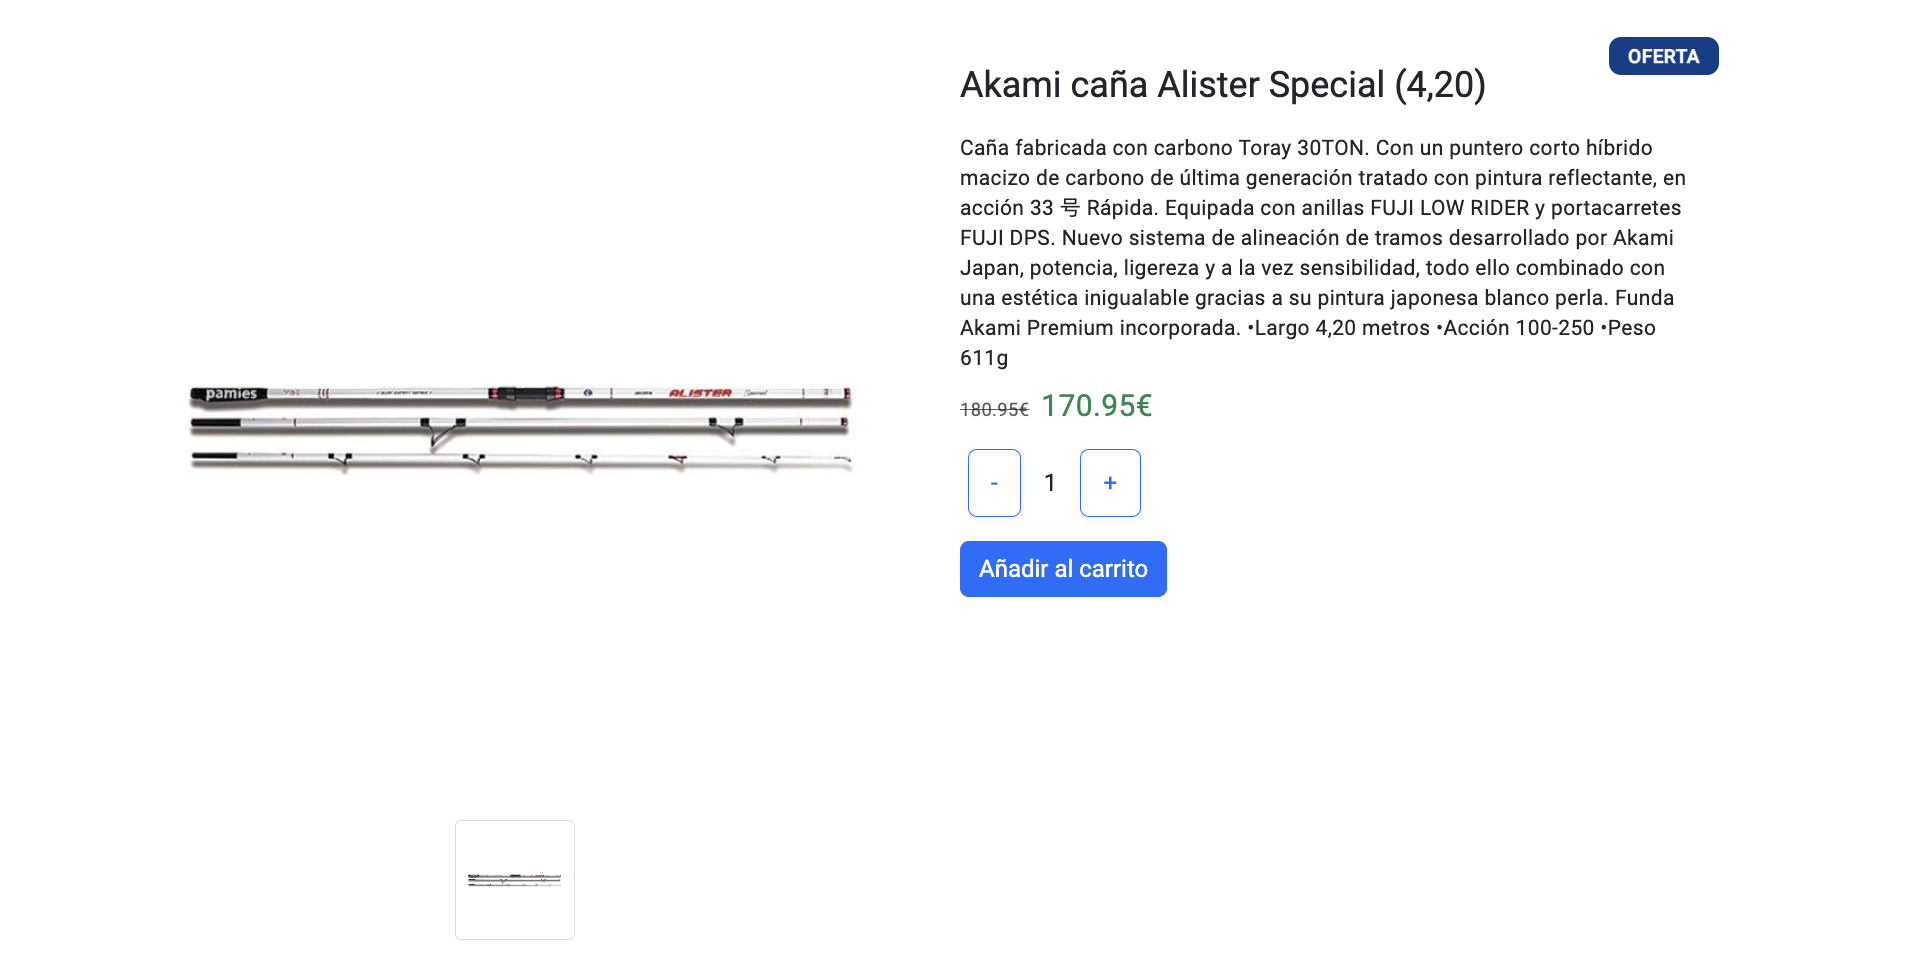
\includegraphics[scale=0.5]{./Images/vistaDetalleProducto.png}
\caption{Vista Detalle de producto} Fuente: Elaboración propia.

\label{fig:fig1}

\end{center}
\end{figure}

A medida que el cliente añade productos, estos se reflejan automáticamente en la vista del carrito. En esta sección se muestra un resumen detallado del pedido, donde es posible visualizar los productos seleccionados, modificar las cantidades o eliminarlos si es necesario. En la parte derecha, se presenta el precio total del pedido junto con un campo donde se puede introducir un código de descuento. Para finalizar, se incluye el botón de 'pagar' que permite al cliente proceder con la confirmación del pedido.


\begin{figure}[H]
\begin{center}
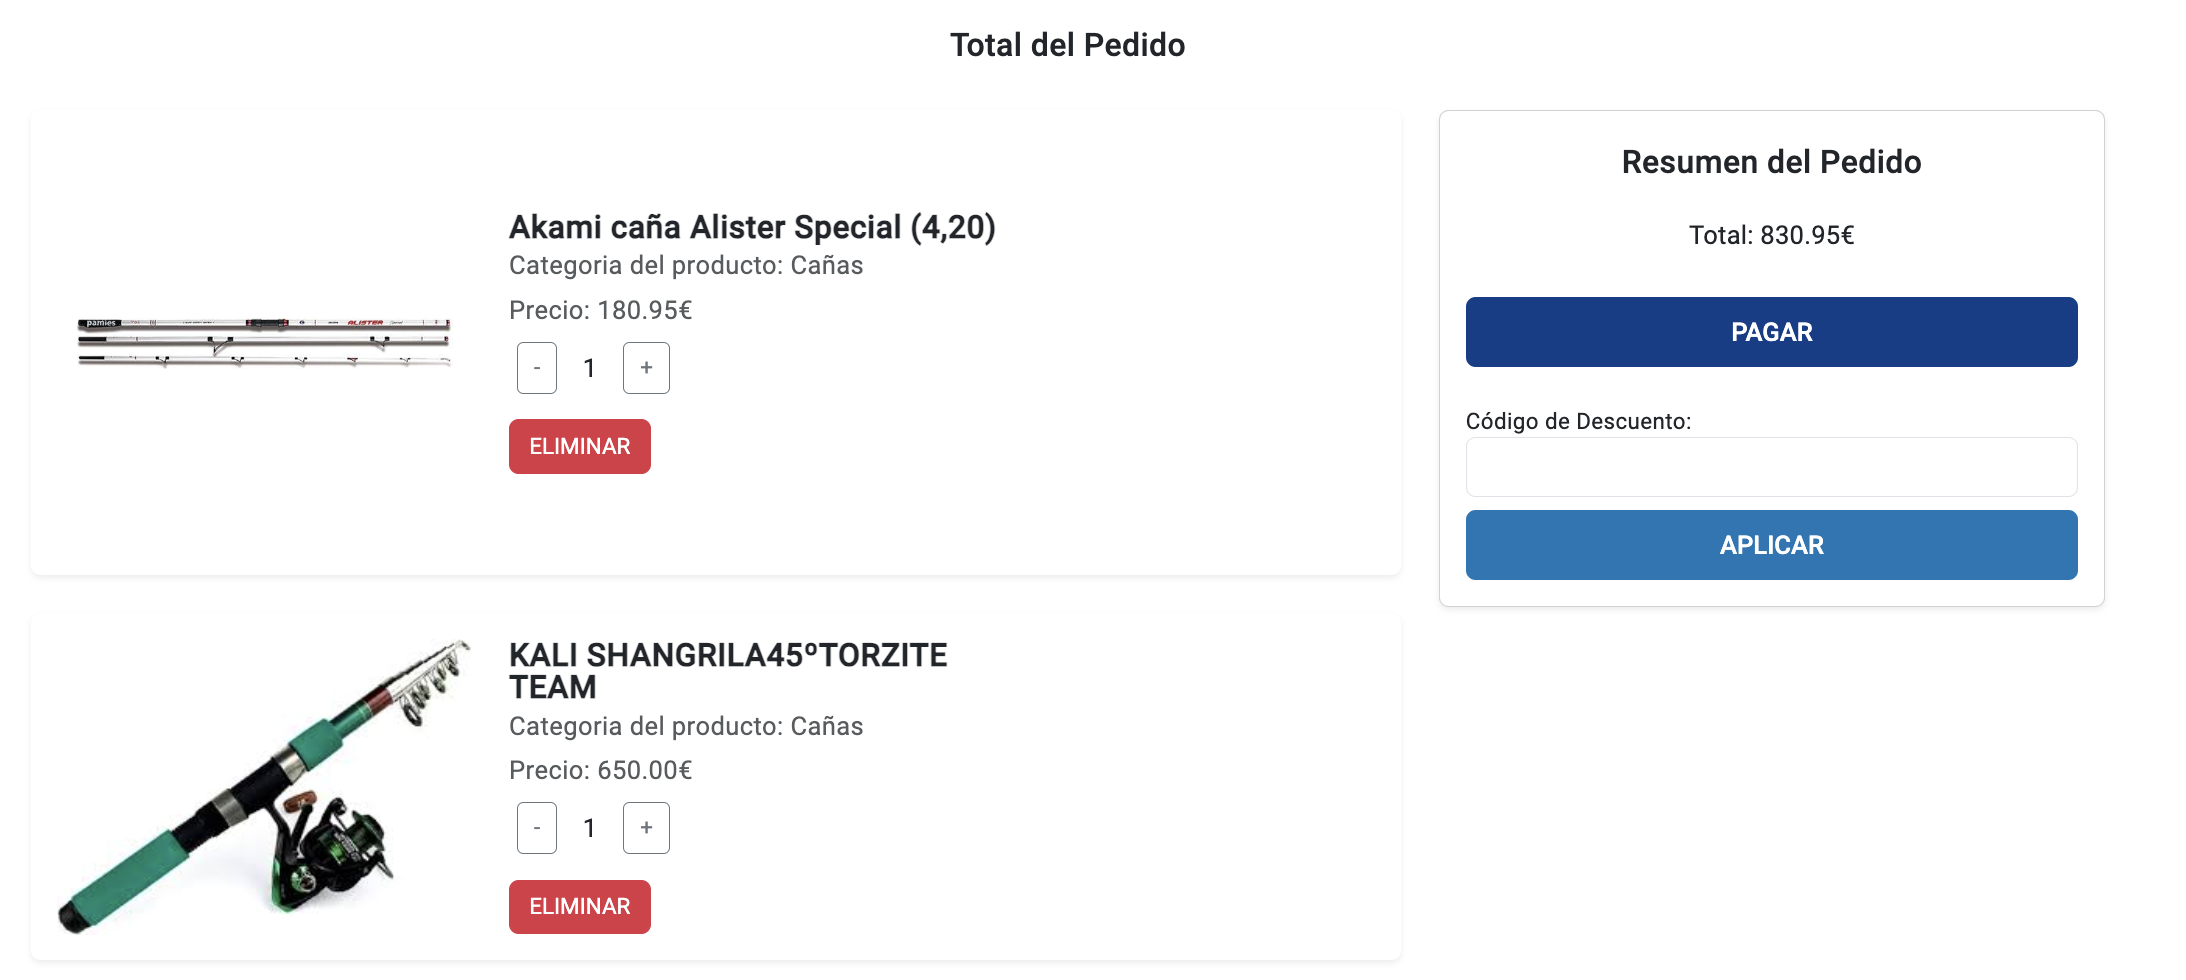
\includegraphics[scale=0.38]{./Images/vistaCarrito.png}
\caption{Vista Carrito de productos} Fuente: Elaboración propia.

\label{fig:fig1}

\end{center}
\end{figure}

Una vez que el cliente confirma el pedido, se genera una pantalla de confirmación en la que se muestra el número de pedido, los productos adquiridos con sus respectivas cantidades y precios, y el total del pedido. Esta misma confirmación es enviada por correo electrónico al cliente para su registro.

\begin{figure}[H]
\begin{center}
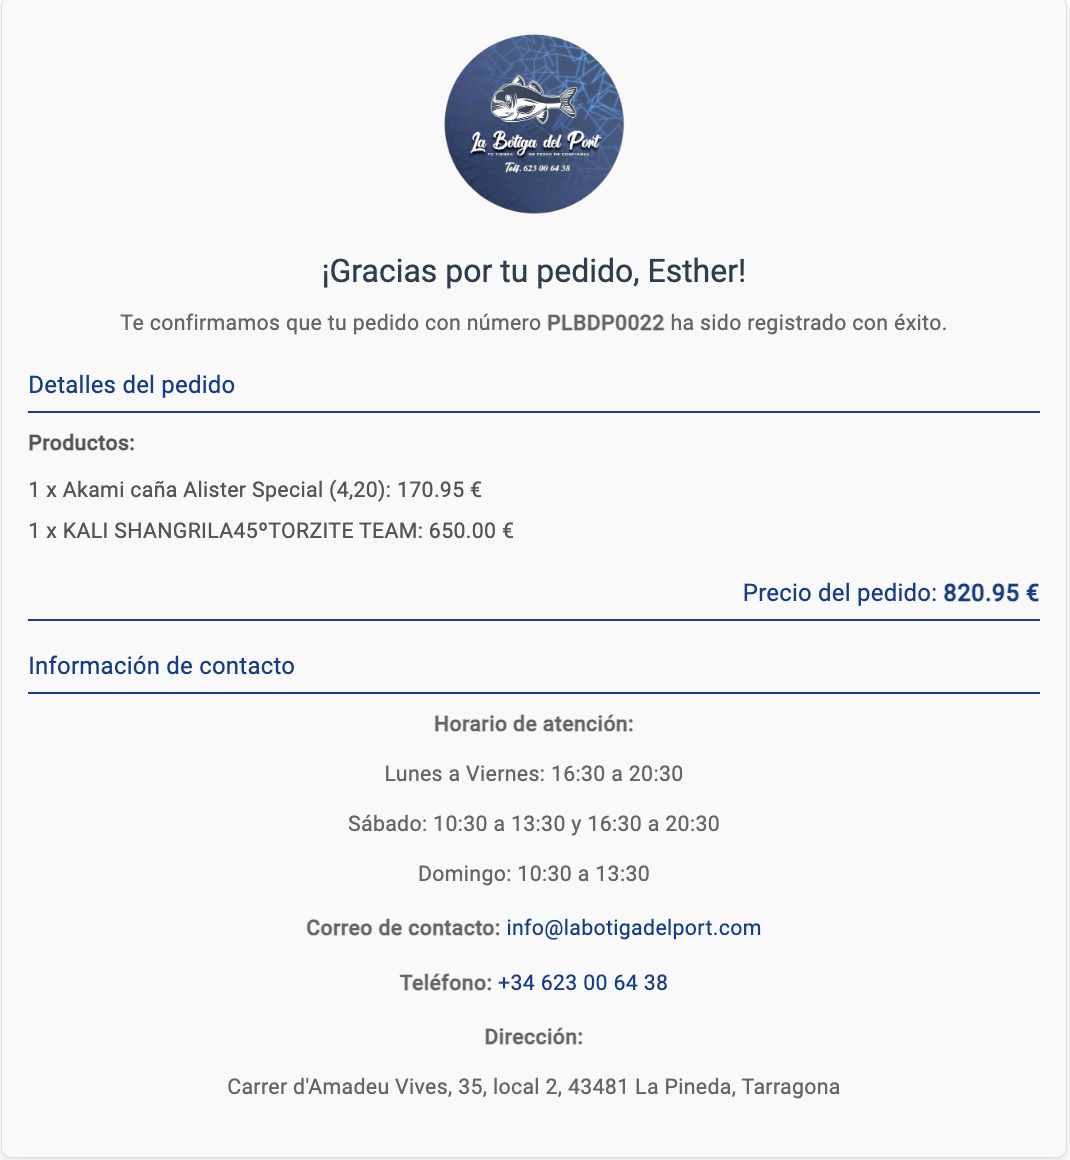
\includegraphics[scale=0.5]{./Images/vistaConfirmacionPedido.png}
\caption{Vista Confirmación del pedido} Fuente: Elaboración propia.

\label{fig:fig1}

\end{center}
\end{figure}

El cliente tiene la opción de ver todos los pedidos que ha realizado en la sección de "Perfil". En este apartado, además de visualizar sus datos personales, puede acceder al historial completo de sus compras, incluyendo detalles de cada pedido, como productos adquiridos, cantidades, precios y fechas. Esto le permite llevar un control de todas sus transacciones a lo largo del tiempo.

\begin{figure}[H]
\begin{center}
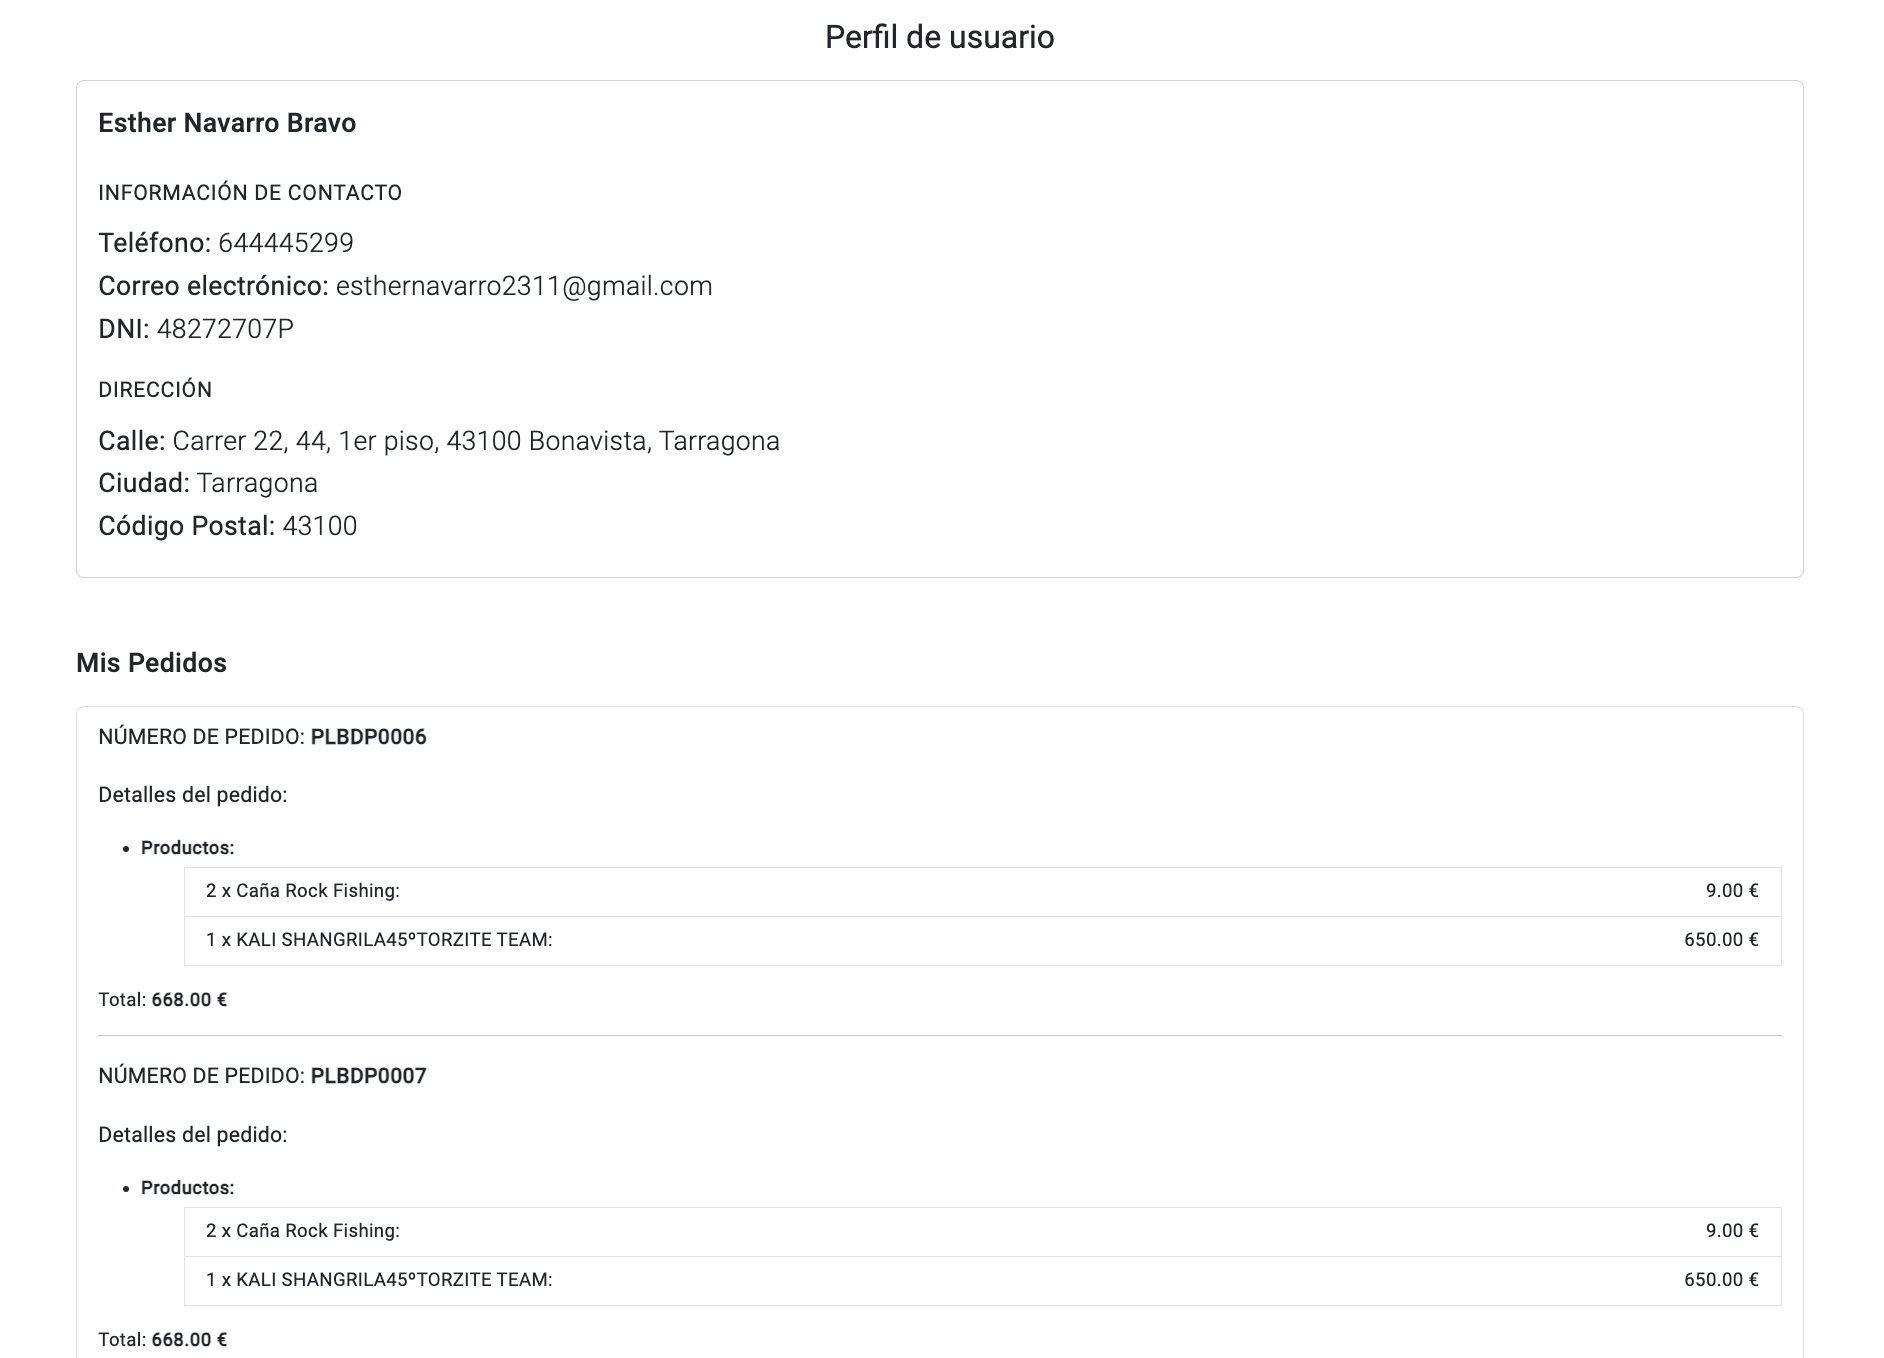
\includegraphics[scale=0.5]{./Images/vistaPerfilUsuario.png}
\caption{Vista Perfil del cliente} Fuente: Elaboración propia.

\label{fig:fig1}

\end{center}
\end{figure}


\subsubsection{Reserva de cebo}\label{subsec5.1.1.3}

La vista de Reserva de cebo permite a los usuarios seleccionar productos relacionados con el cebo de pesca de manera sencilla. Cada producto se muestra con su nombre, imagen representativa y precio. El usuario tiene la opción de elegir la cantidad de cada producto que desea adquirir y debe seleccionar una fecha de recogida antes de proceder. Esta interfaz asegura que toda la información relevante esté fácilmente accesible, facilitando la navegación y el proceso de reserva.

\begin{figure}[H]
\begin{center}
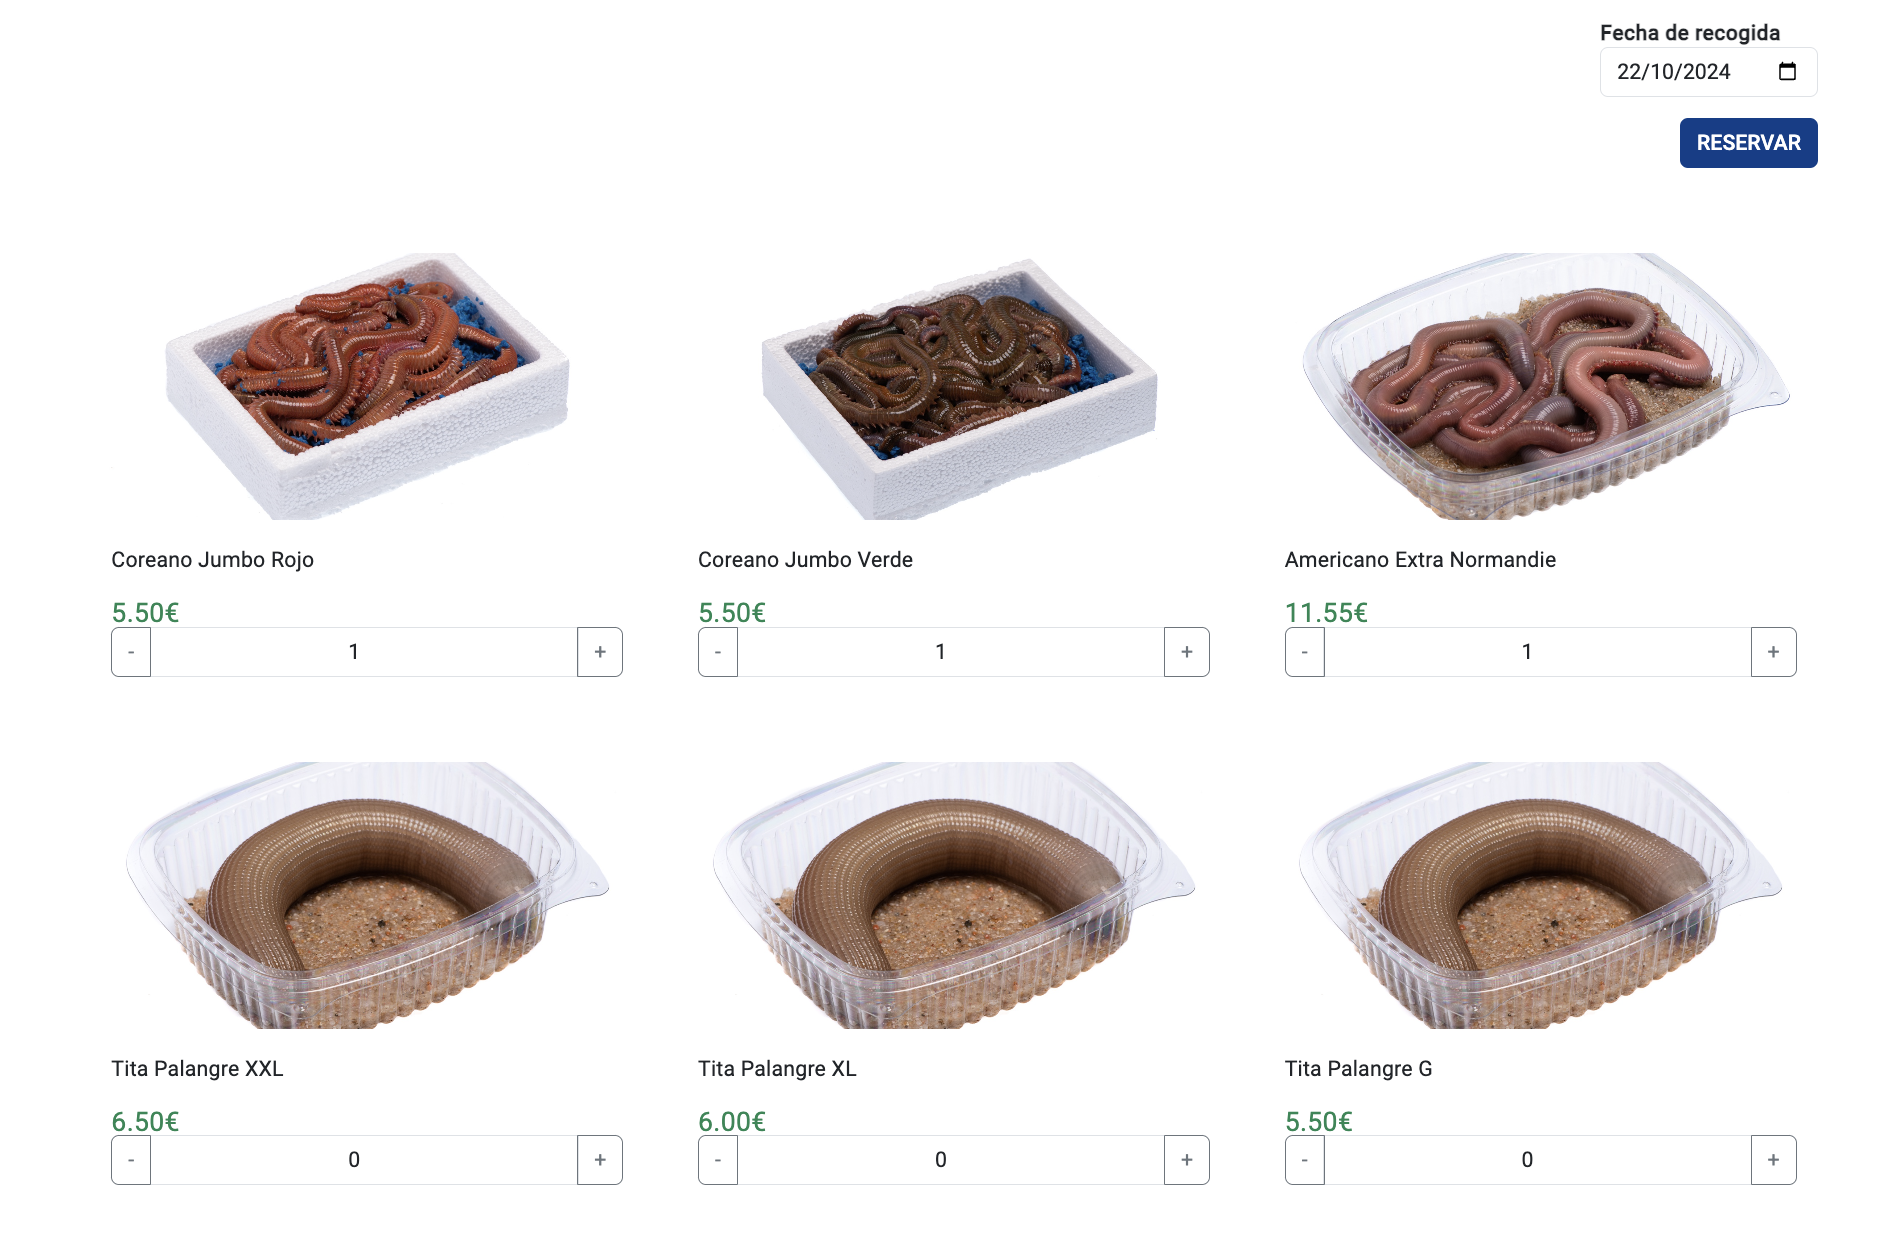
\includegraphics[scale=0.5]{./Images/vistaReservaCebo.png}
\caption{Vista Reserva de cebo} Fuente: Elaboración propia.

\label{fig:fig1}

\end{center}
\end{figure}

Una vez seleccionados los productos, la vista presenta un resumen de la reserva, en el que se detalla cada artículo, incluyendo las cantidades elegidas. Desde esta sección, los usuarios pueden ajustar la cantidad de cada producto si lo consideran necesario. El precio total de la reserva se calcula y se muestra automáticamente, brindando una visión clara del coste final. Cuando el usuario está satisfecho con su selección, puede proceder a confirmar la reserva.

\begin{figure}[H]
\begin{center}
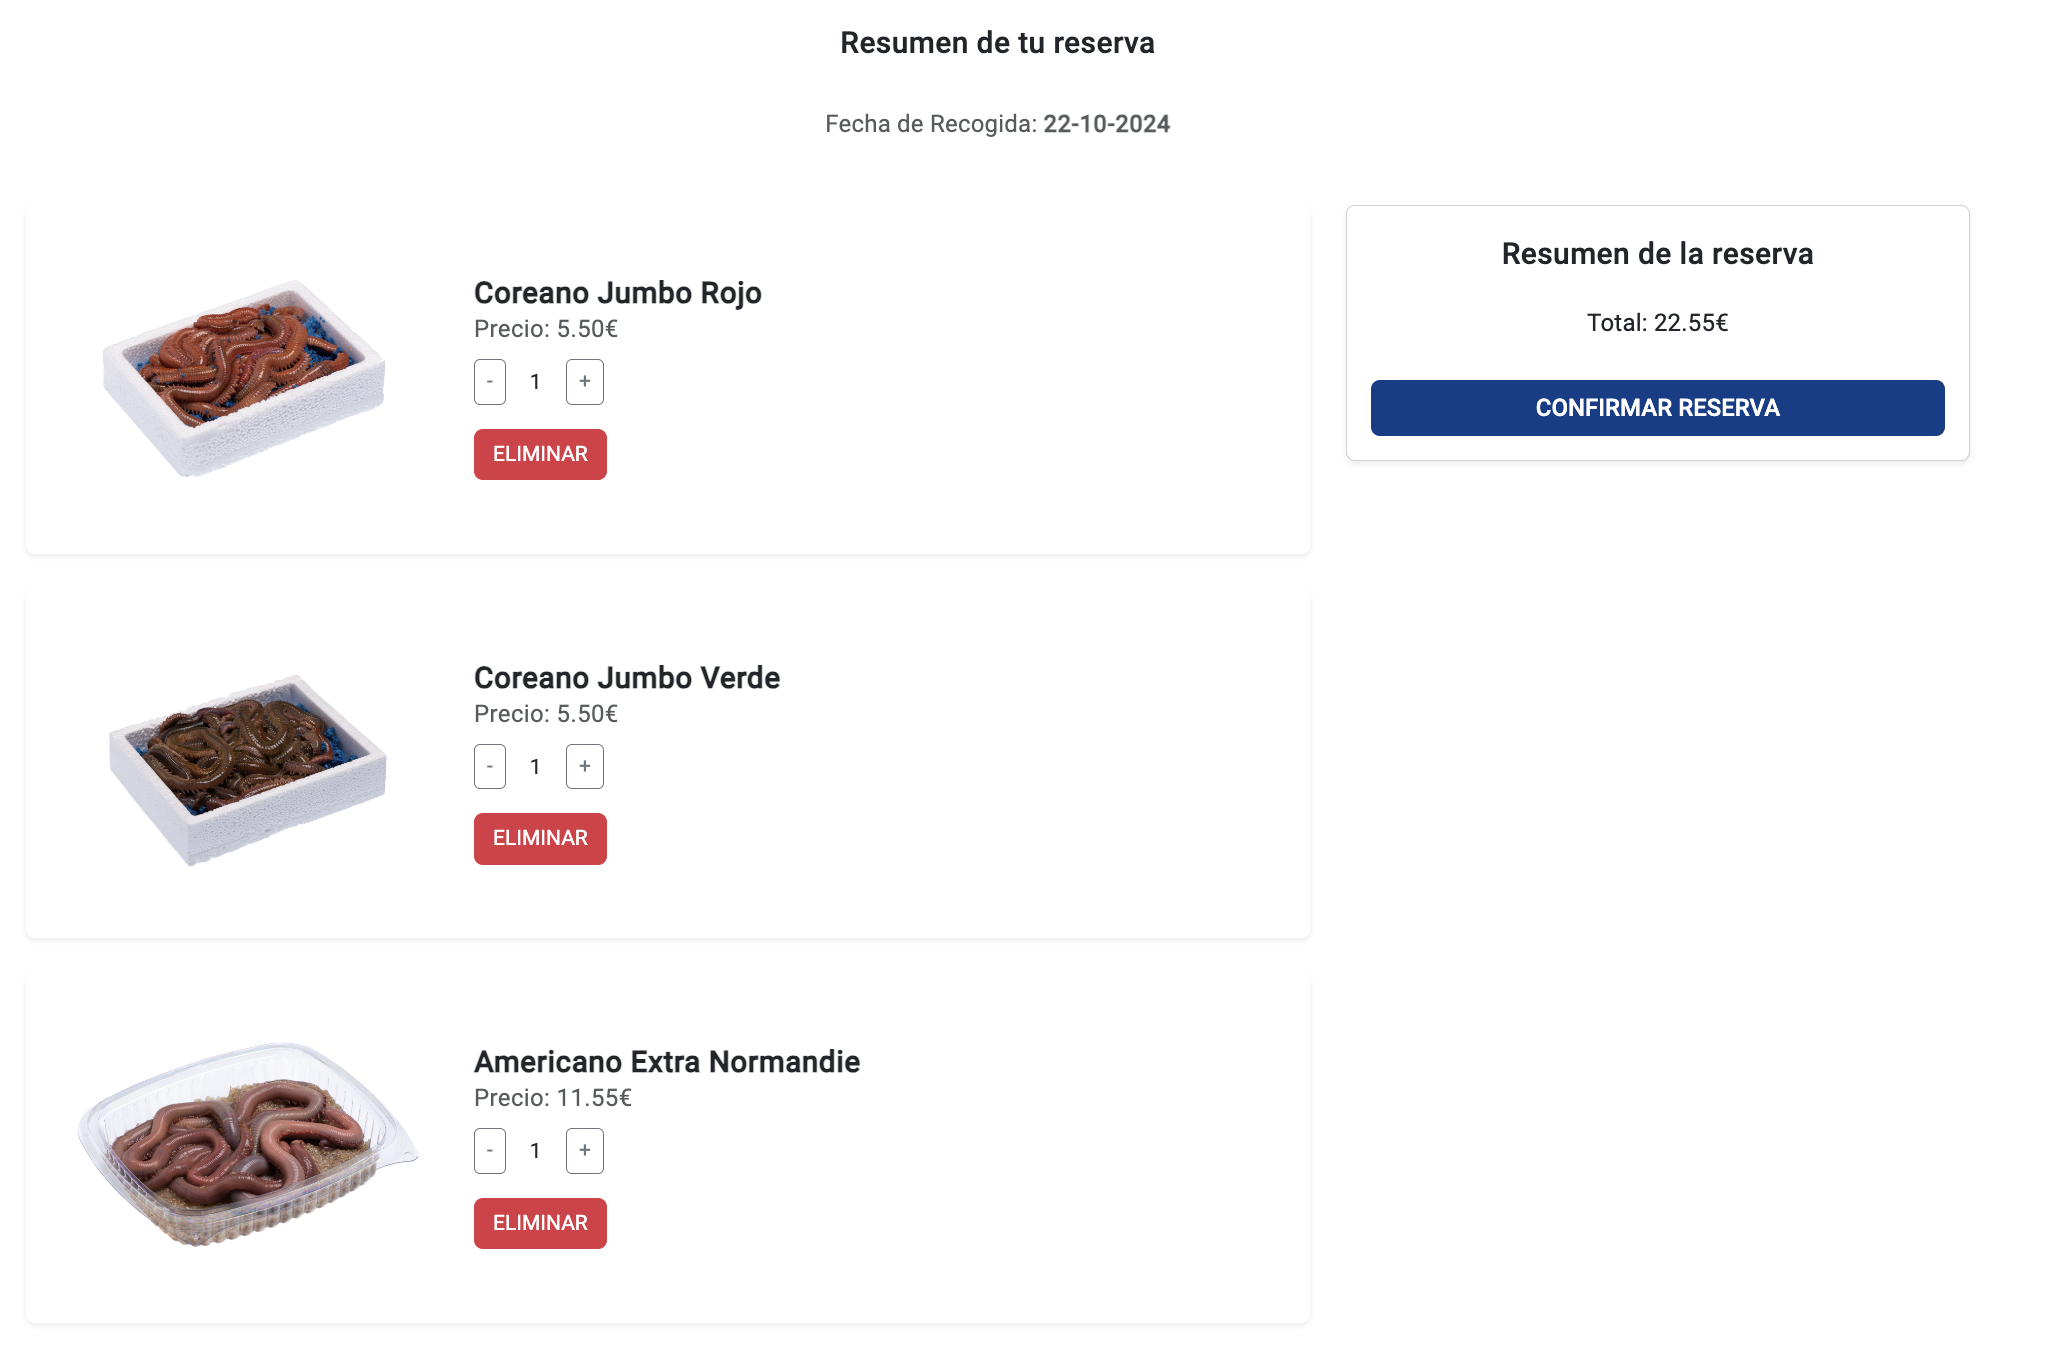
\includegraphics[scale=0.5]{./Images/vistaResumenReservaCebo.png}
\caption{Vista Resumen reserva de cebo} Fuente: Elaboración propia.

\label{fig:fig1}

\end{center}
\end{figure}

Después de confirmar la reserva, el sistema genera un resumen completo de la misma, mostrando los productos seleccionados, la cantidad de cada uno y el precio total. Este resumen se presenta tanto en pantalla como en un correo electrónico que se envía automáticamente al cliente, asegurando que el usuario tenga un registro de su pedido.

\begin{figure}[H]
\begin{center}
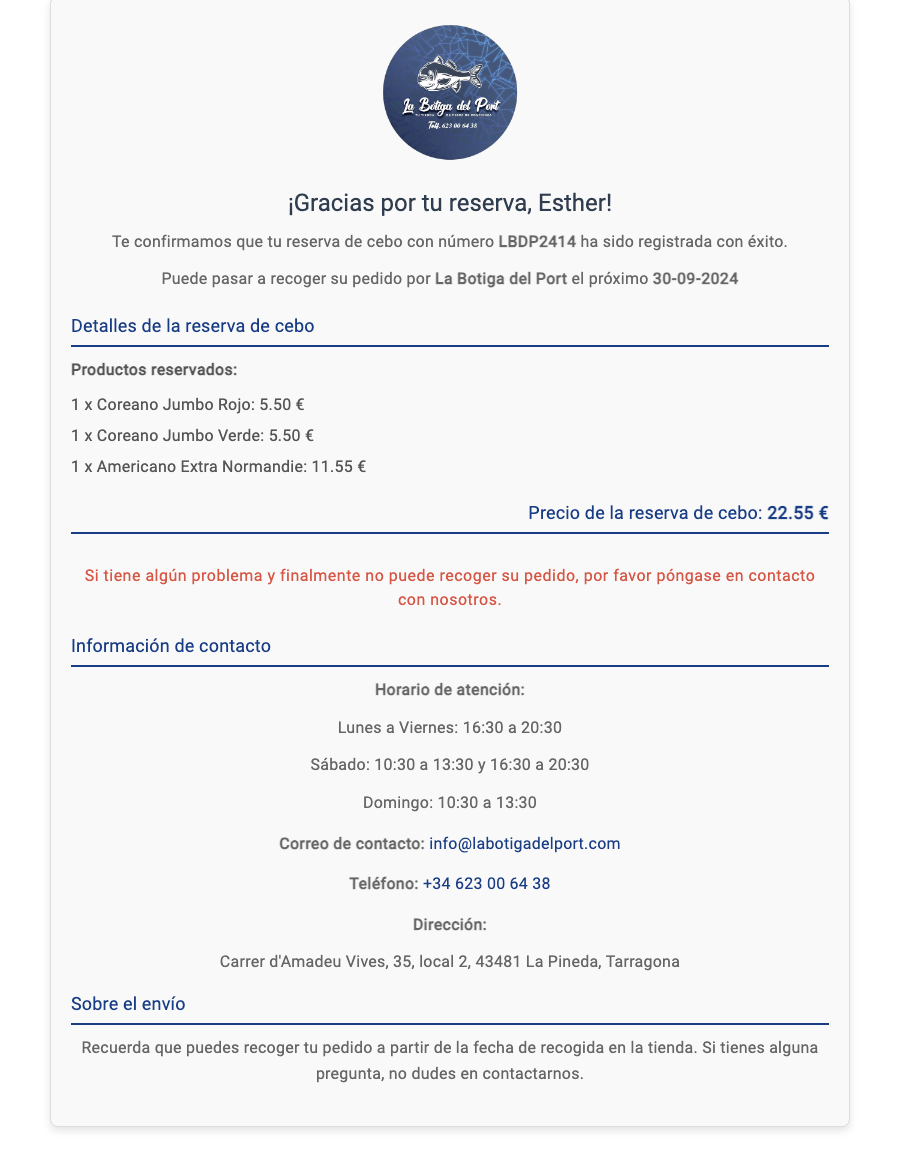
\includegraphics[scale=0.7]{./Images/vistaConfirmacionReservaCebo.png}
\caption{Vista Confirmación reserva de cebo} Fuente: Elaboración propia.

\label{fig:fig1}

\end{center}
\end{figure}

\subsubsection{Página principal}\label{subsec5.1.1.4}

En la página principal, se presentan tres módulos clave para una experiencia de usuario atractiva y funcional. El primer módulo es un banner informativo que incluye un título, un subtítulo y un botón que dirige al cliente a una página o enlace específico. Este banner es ideal para destacar las promociones vigentes o para redirigir a los usuarios a páginas importantes, como ofertas especiales, lanzamientos de productos o eventos destacados.

\begin{figure}[H]
\begin{center}

\includegraphics[scale=0.4]{./Images/vistaBanner.png}
\caption{Banner informativo} Fuente: Elaboración propia.

\label{fig:fig1}

\end{center}
\end{figure}

El segundo módulo es un carrusel que muestra los seis productos más vendidos de la tienda. Cada producto se presenta con su imagen, nombre y precio, ofreciendo una vista clara y atractiva de los artículos más populares. Al hacer clic en cualquiera de estos productos, el cliente es redirigido a la página de detalles del producto, donde puede obtener más información y realizar la compra.

\begin{figure}[H]
\begin{center}
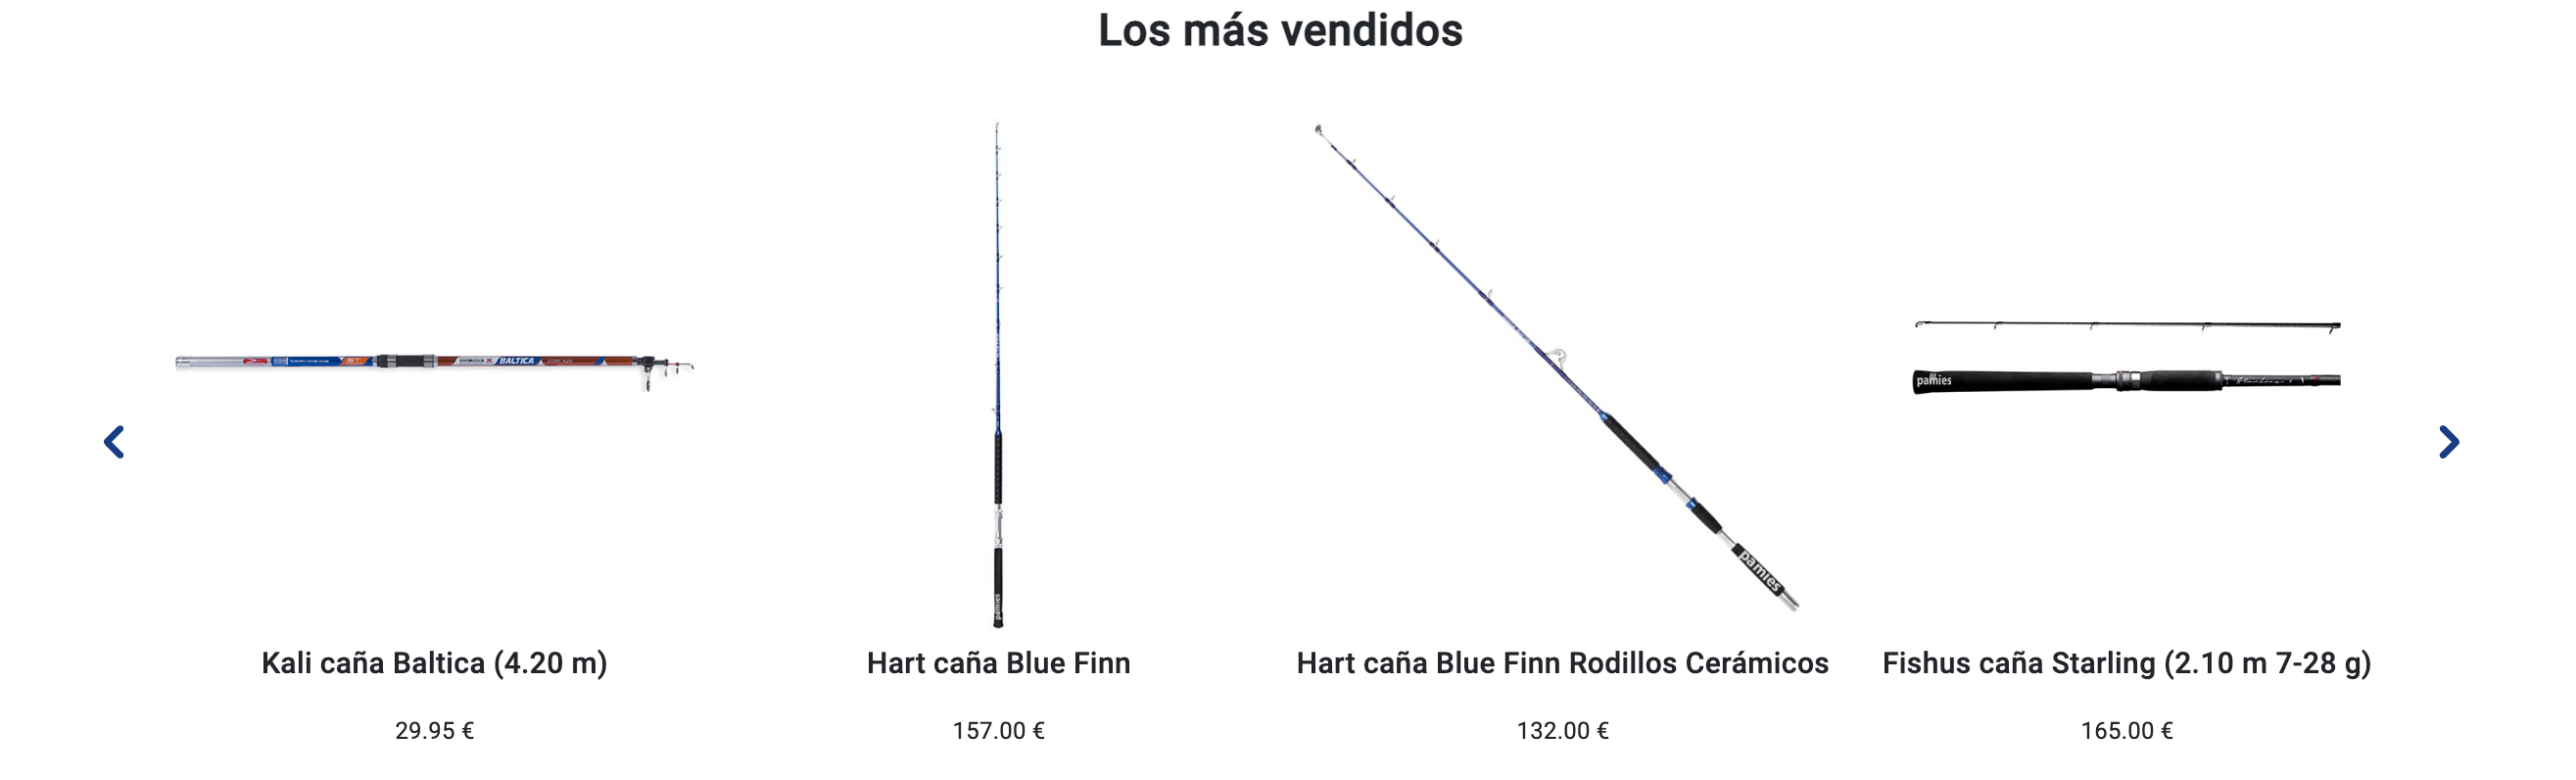
\includegraphics[scale=0.35]{./Images/vistaCarrusel.png}
\caption{Carrusel de productos} Fuente: Elaboración propia.

\label{fig:fig1}

\end{center}
\end{figure}

El tercer módulo consta de tres tarjetas que representan las categorías de novedades, ofertas y liquidaciones. Estas tarjetas permiten un acceso rápido a las páginas específicas de cada categoría, mostrando los productos que cumplen con estas características. Al hacer clic en cada tarjeta, el usuario es dirigido a la página correspondiente, donde podrá explorar los productos disponibles bajo novedades, ofertas o liquidaciones, según su interés.

\begin{figure}[H]
\begin{center}
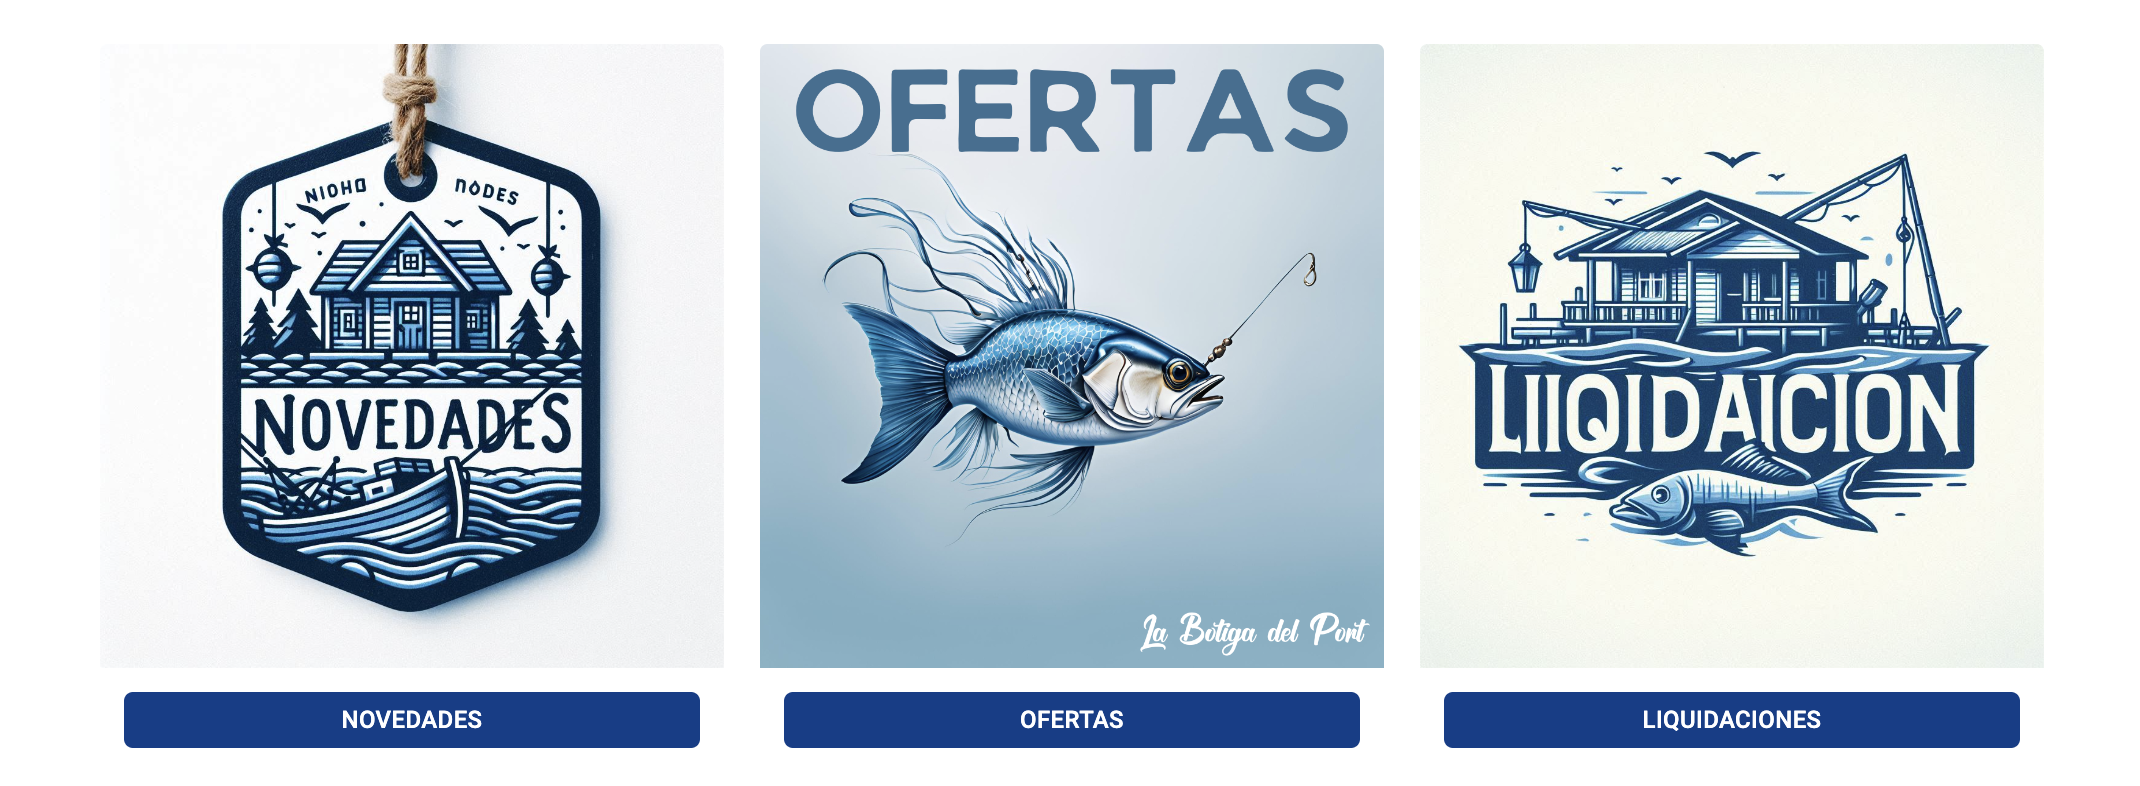
\includegraphics[scale=0.4]{./Images/vistaCards.png}
\caption{Tarjetas de acceso rápido} Fuente: Elaboración propia.

\label{fig:fig1}

\end{center}
\end{figure}



\subsection{Vista para el adminstrador}\label{subsec5.1.2}

\subsubsection{Productos y pedidos}\label{subsec5.1.2.1}
En la vista de gestión de productos, en la parte superior derecha se encuentra un botón que permite añadir un nuevo producto al catálogo. Debajo de este, se muestran todos los productos disponibles, cada uno con su información relevante, como nombre, precio y categoría. Junto a cada producto, el administrador dispone de botones para eliminar el producto, editarlo, y dos botones adicionales para marcar o desmarcar el producto como novedad o como liquidación, facilitando la organización y promoción del inventario.

\begin{figure}[H]
\begin{center}
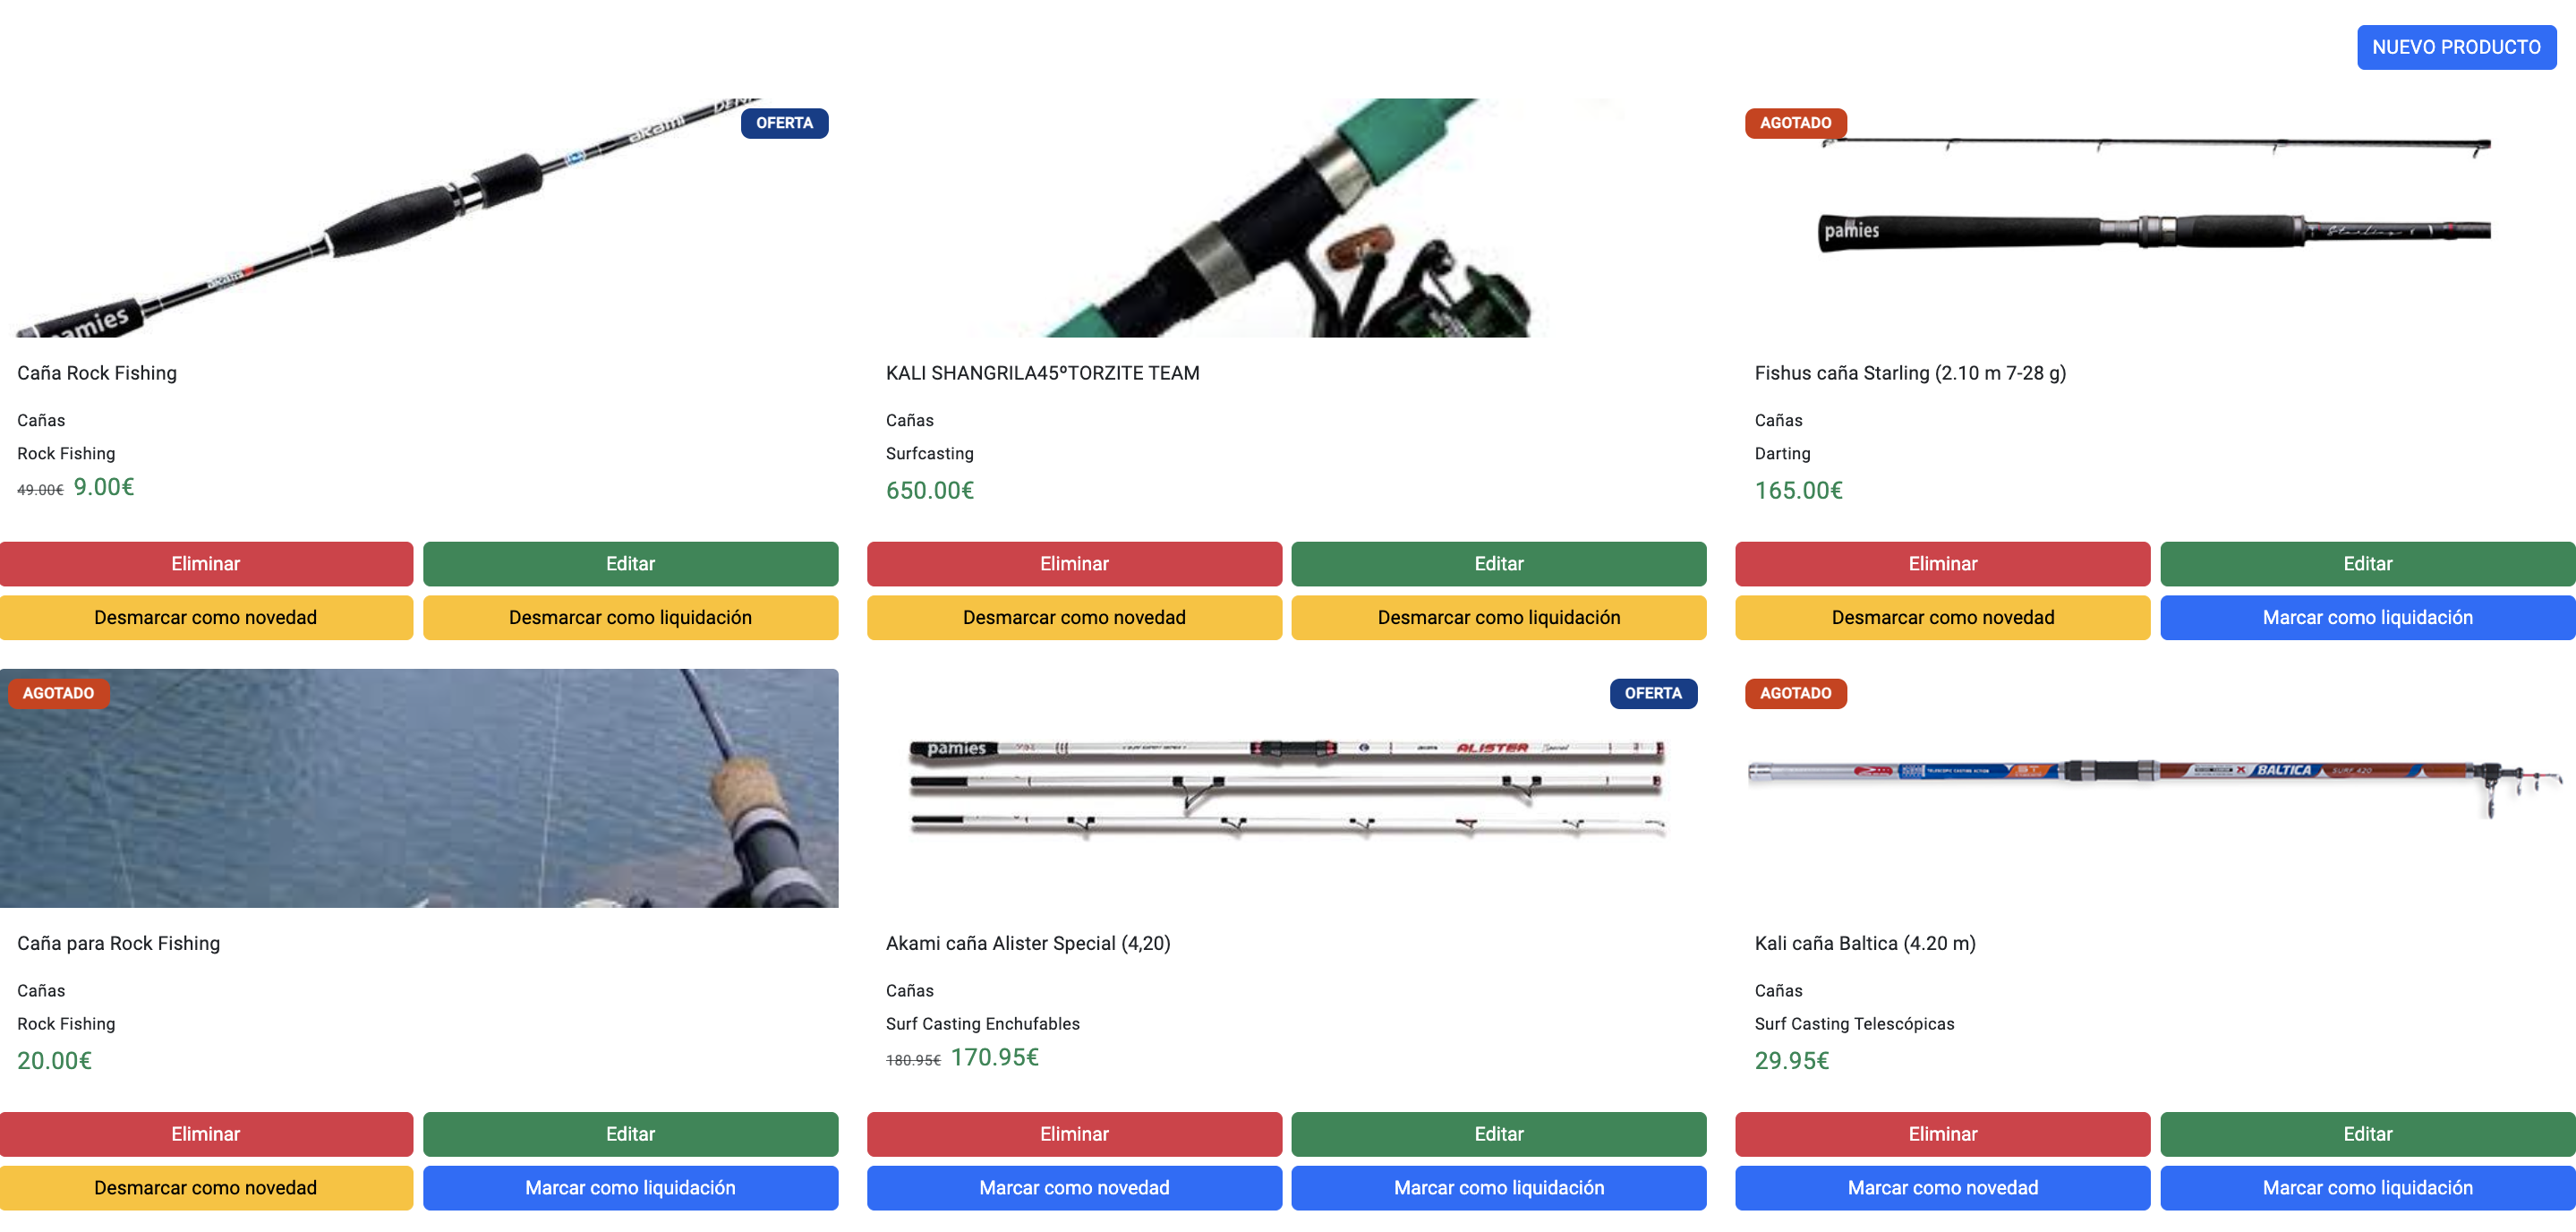
\includegraphics[scale=0.35]{./Images/vistaAdminProductos.png}
\caption{Vista Gestión de productos} Fuente: Elaboración propia.

\label{fig:fig1}

\end{center}
\end{figure}

Cuando se desea añadir un nuevo producto, se muestra un formulario en el que se deben completar todos los campos necesarios para crear el producto, como su nombre, precio, descripción, categoría, etc. Además, se incluye un campo para subir la imagen principal del producto, así como un campo adicional para añadir imágenes secundarias que ayuden a mostrar el producto desde diferentes ángulos o contextos.

\begin{figure}[H]
\begin{center}
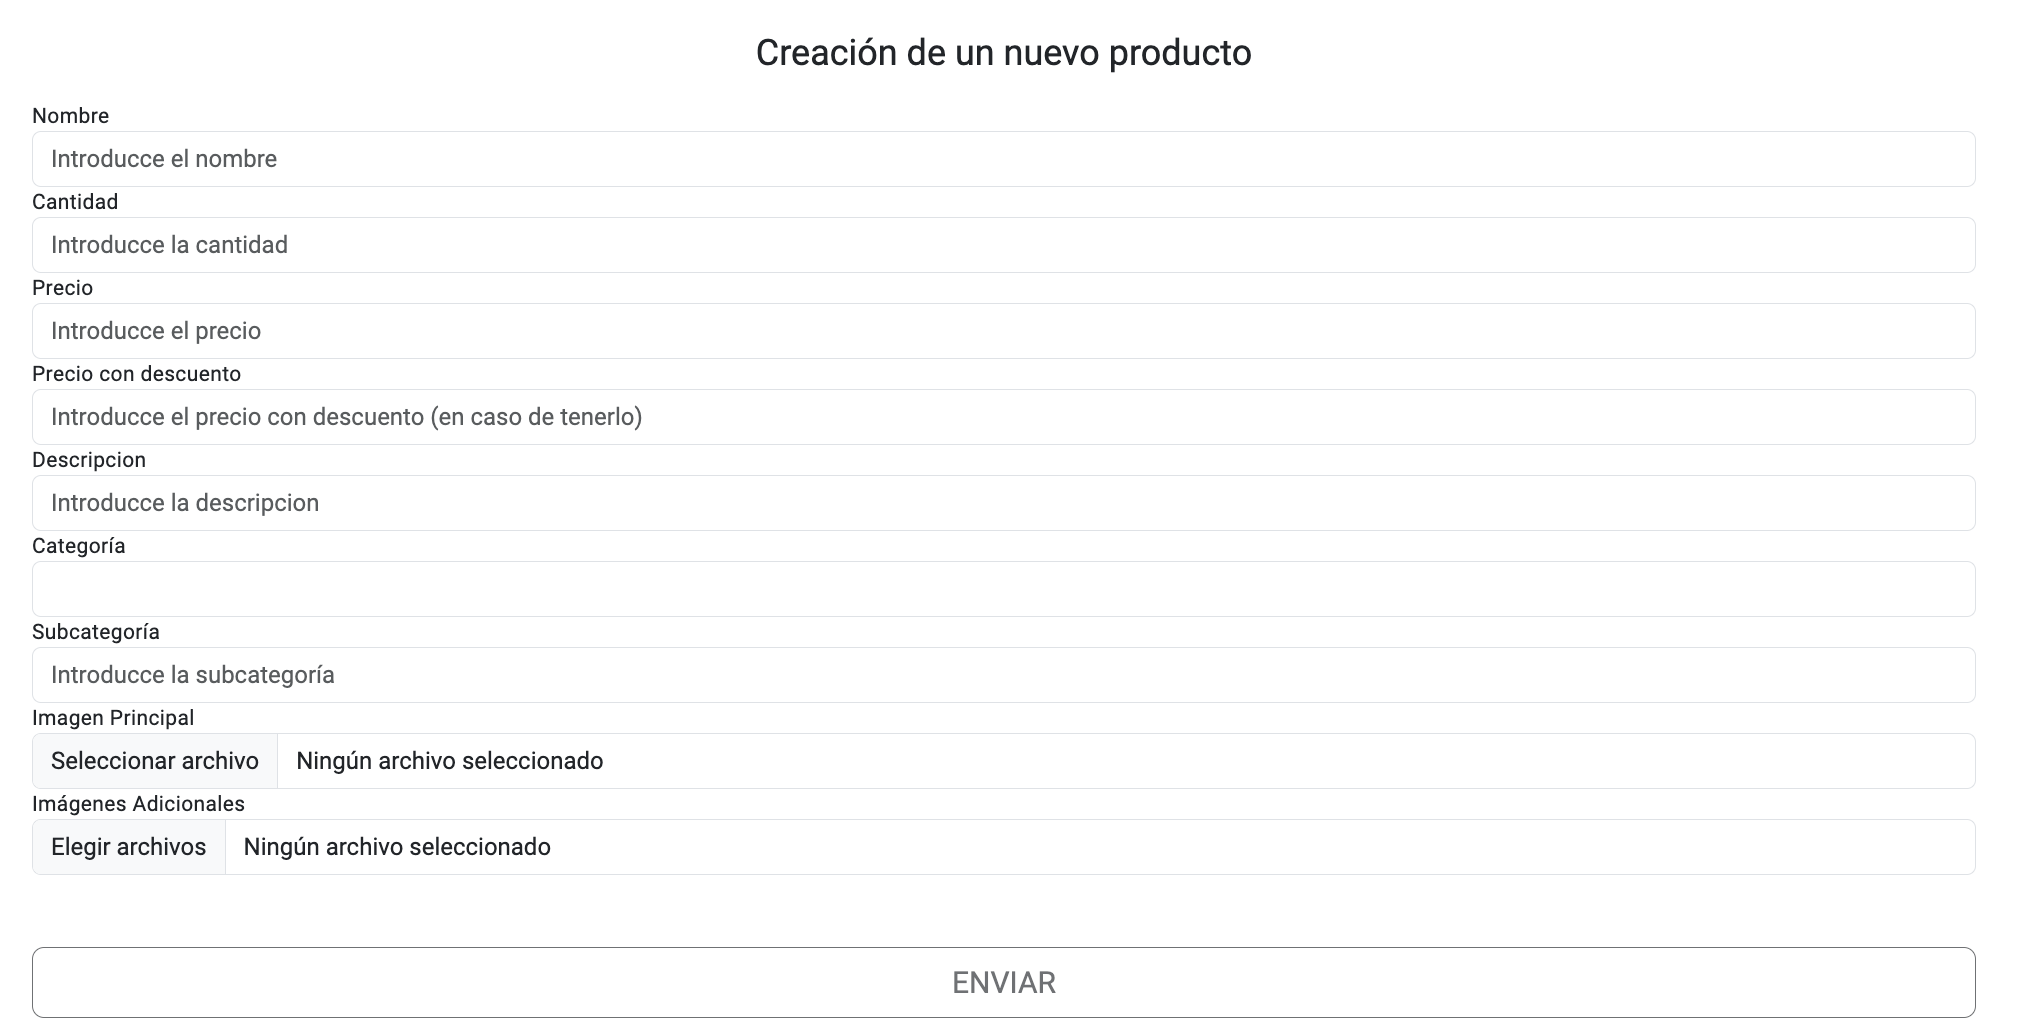
\includegraphics[scale=0.5]{./Images/vistaAdminNuevoProducto.png}
\caption{Vista Nuevo producto} Fuente: Elaboración propia.

\label{fig:fig1}

\end{center}
\end{figure}

En el caso de editar un producto existente, el administrador accede al mismo formulario de creación, pero esta vez aparece rellenado con los datos actuales del producto que se desea modificar. Aquí se pueden ajustar todos los detalles del producto, incluyendo su imagen principal y las imágenes adicionales, para mantener el catálogo actualizado.

\vspace{0.5cm}

Por último, en el apartado de gestión de pedidos, se muestra una lista con todos los pedidos realizados, incluyendo el número de pedido, el nombre del cliente, su teléfono y correo electrónico, la cantidad de productos, los productos solicitados, y el precio total del pedido. Además, se puede utilizar un buscador para filtrar los pedidos por cliente, permitiendo ver rápidamente todos los pedidos que ha realizado un cliente en particular.

\begin{figure}[H]
\begin{center}
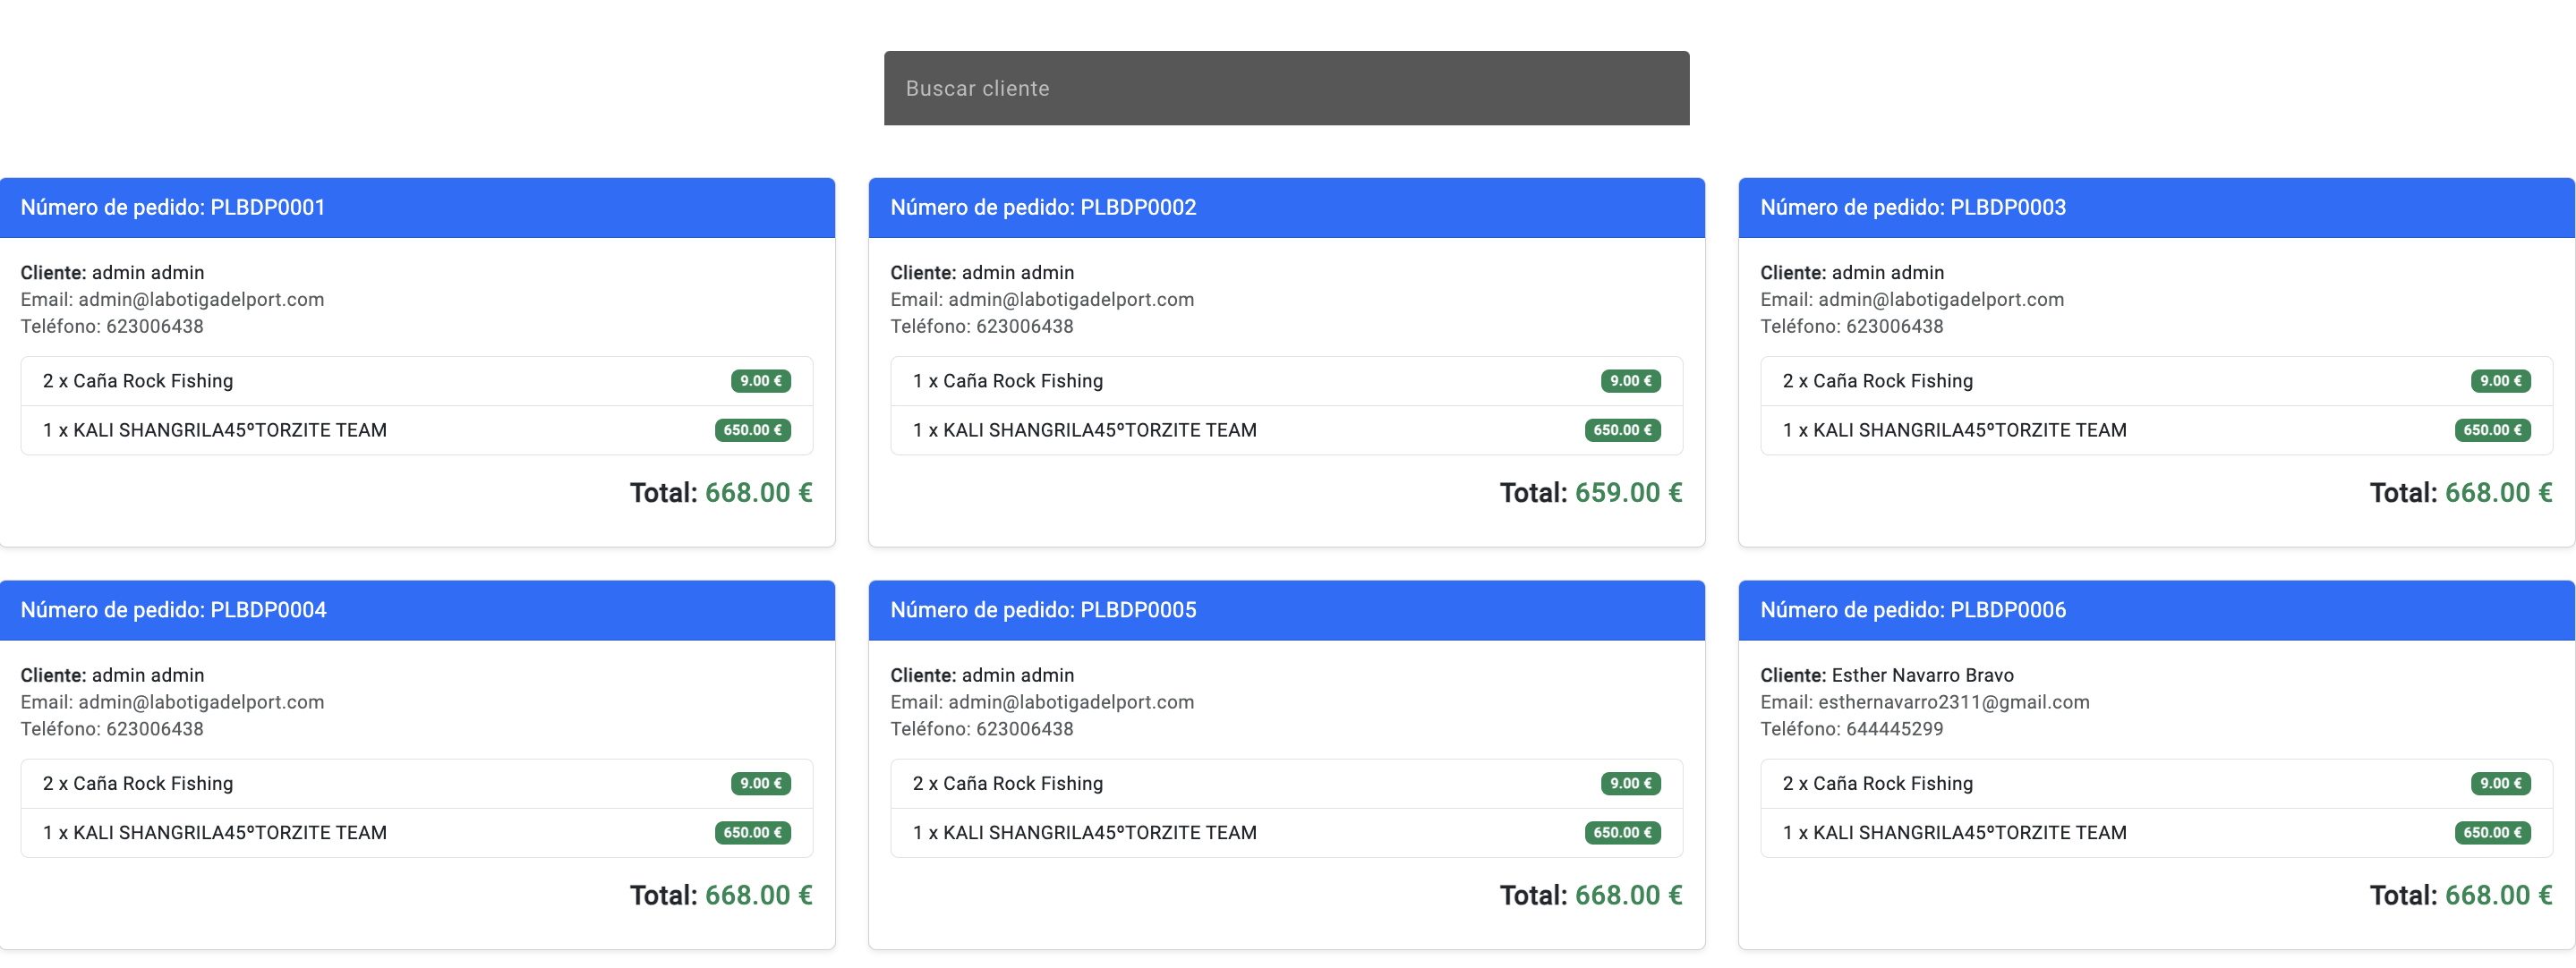
\includegraphics[scale=0.35]{./Images/vistaAdminPedidos.png}
\caption{Vista Nuevo producto} Fuente: Elaboración propia.

\label{fig:fig1}

\end{center}
\end{figure}

\subsubsection{Reserva de cebo}\label{subsec5.1.2.2}
La vista de gestión de reservas de cebo para el administrador presenta una pantalla donde se listan todas las reservas de cebo realizadas por los clientes. En la parte superior, se incluye un buscador que permite filtrar las reservas por el nombre del cliente, mostrando solo las relacionadas con dicho usuario. Además, se han implementado pestañas (tabs) que permiten al administrador alternar entre las reservas "todas", "futuras" o "pasadas", facilitando la organización y visualización de las mismas.

\vspace{0.5cm}

En cada reserva se muestra información clave, como el número de reserva, la fecha de recogida, los datos básicos del cliente (como nombre, teléfono y correo electrónico), así como una lista detallada de los productos reservados con sus respectivas cantidades y precios. Junto a cada reserva, se incluyen dos botones de acción: uno para eliminar la reserva si es necesario, y otro para marcar la reserva como recogida, actualizando así el estado de la misma en el sistema.

\begin{figure}[H]
\begin{center}
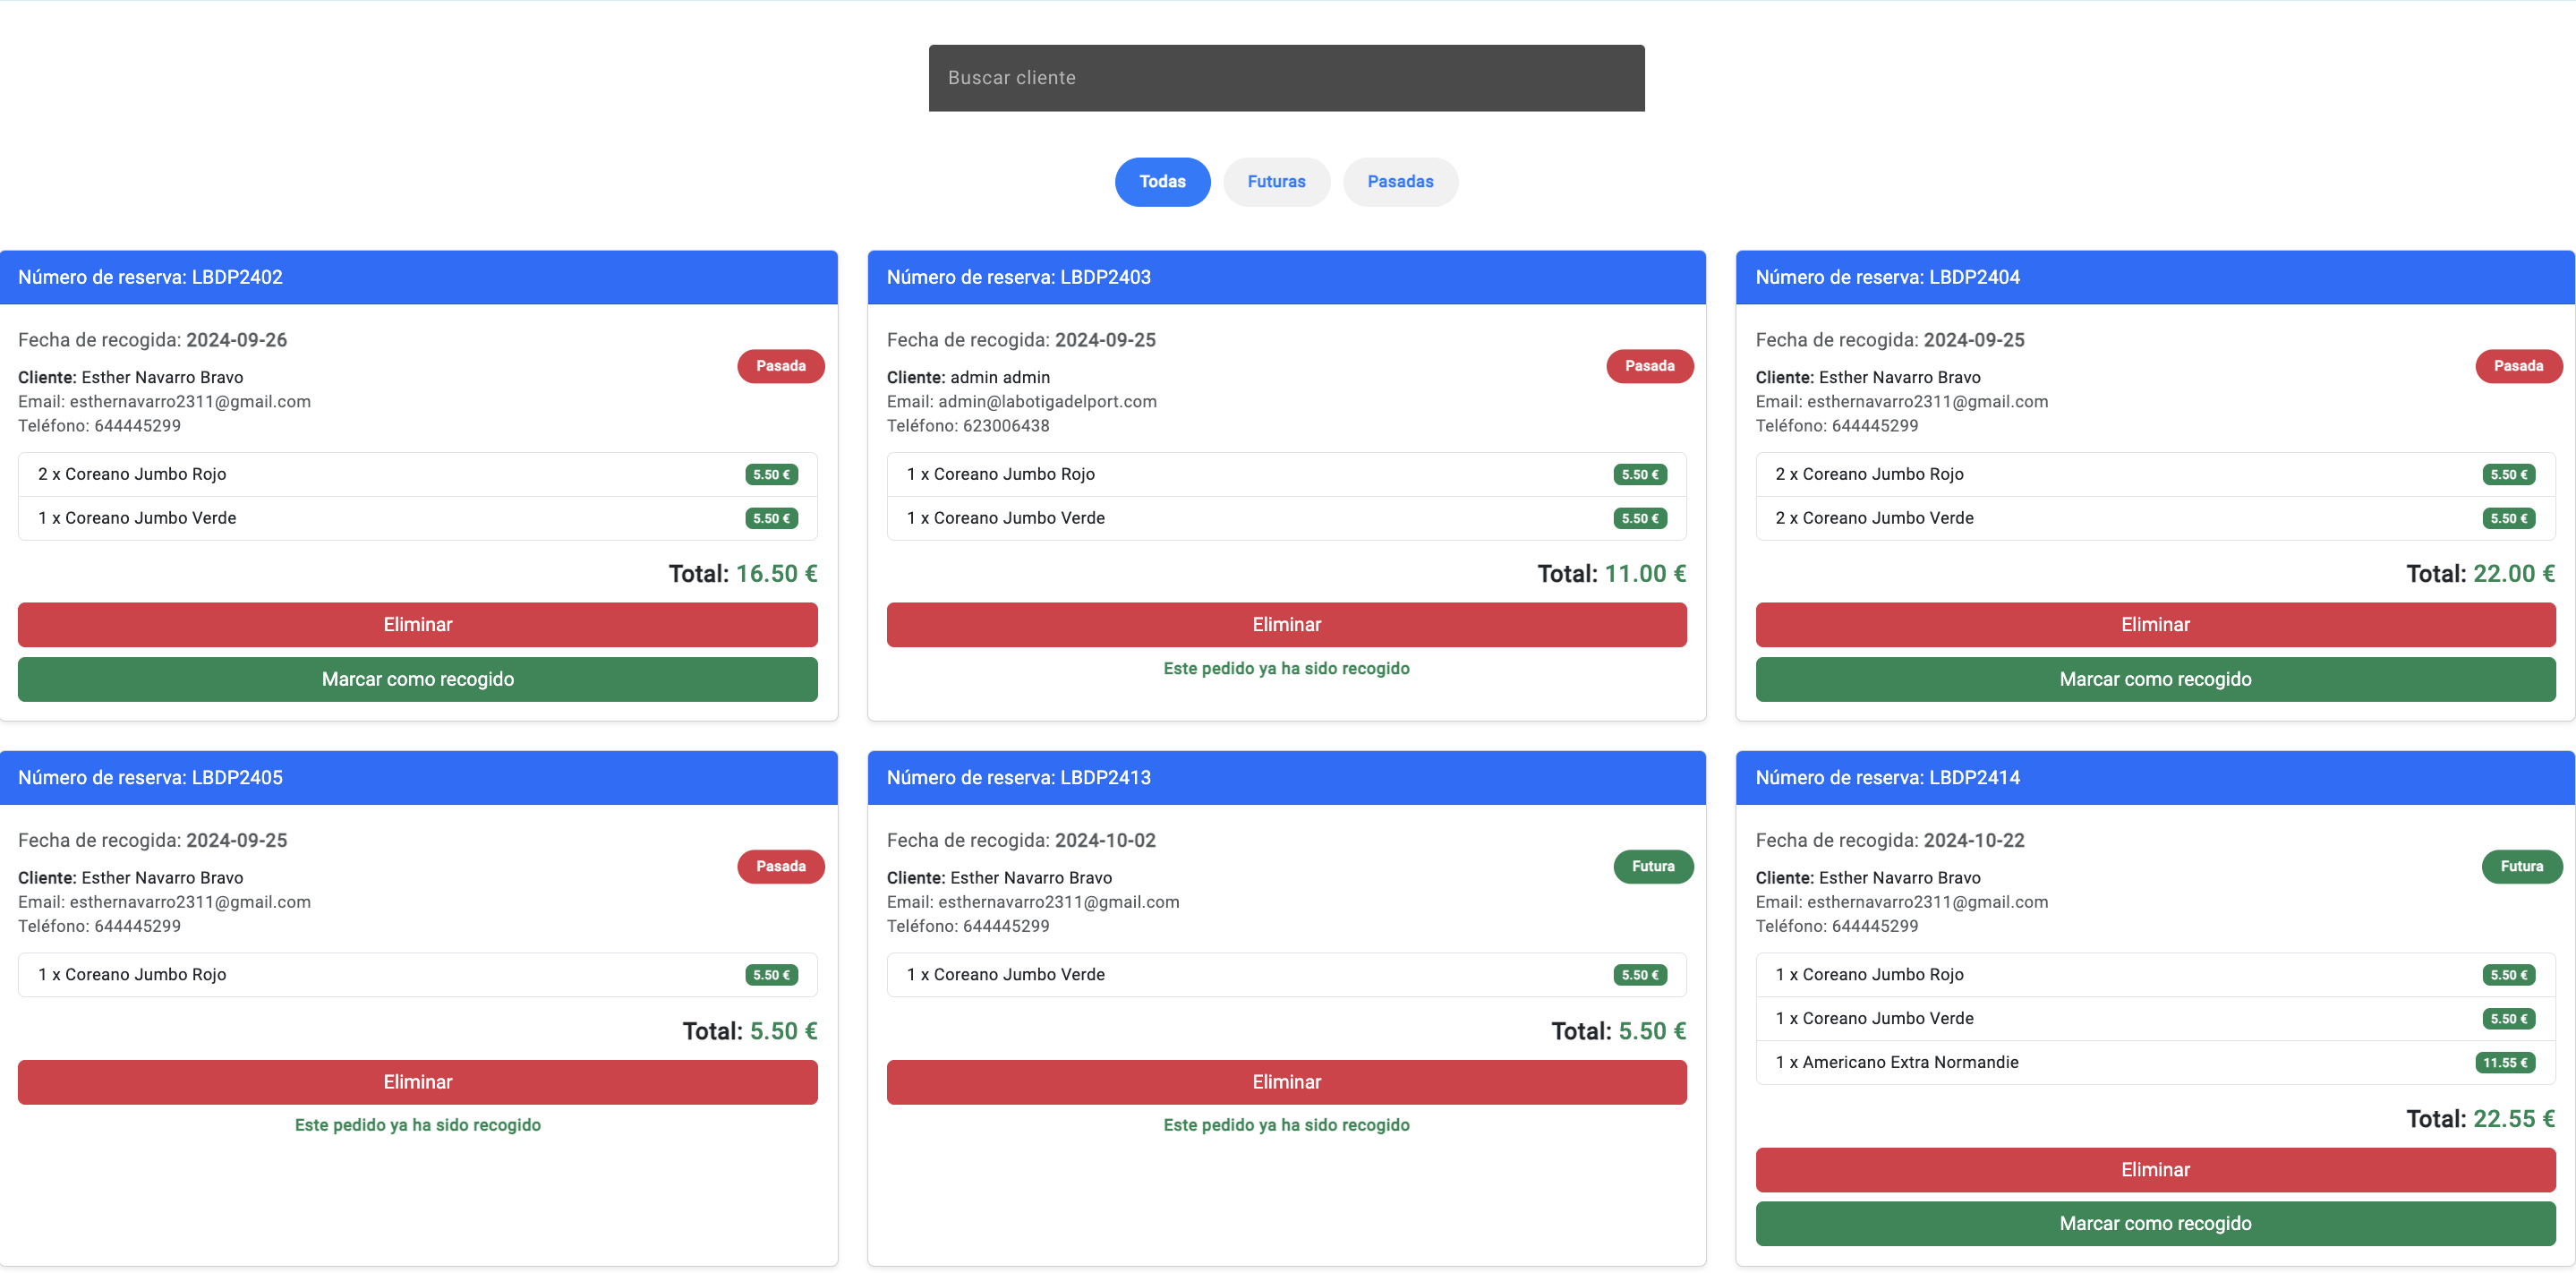
\includegraphics[scale=0.30]{./Images/vistaAdminReservas.png}
\caption{Vista gestión de reserva de cebo} Fuente: Elaboración propia.

\label{fig:fig1}

\end{center}
\end{figure}


\subsubsection{Página principal}\label{subsec5.1.2.3}

En la página principal del administrador, se ofrece la posibilidad de modificar y gestionar los tres módulos clave visibles para los clientes. El primer módulo es el banner informativo, donde el administrador puede crear un nuevo banner, editarlo, eliminarlo o marcarlo como principal para que sea el que aparezca de manera destacada en la página principal. Esto permite un control flexible sobre las promociones o enlaces que se quieran resaltar en la tienda.

\begin{figure}[H]
\begin{center}
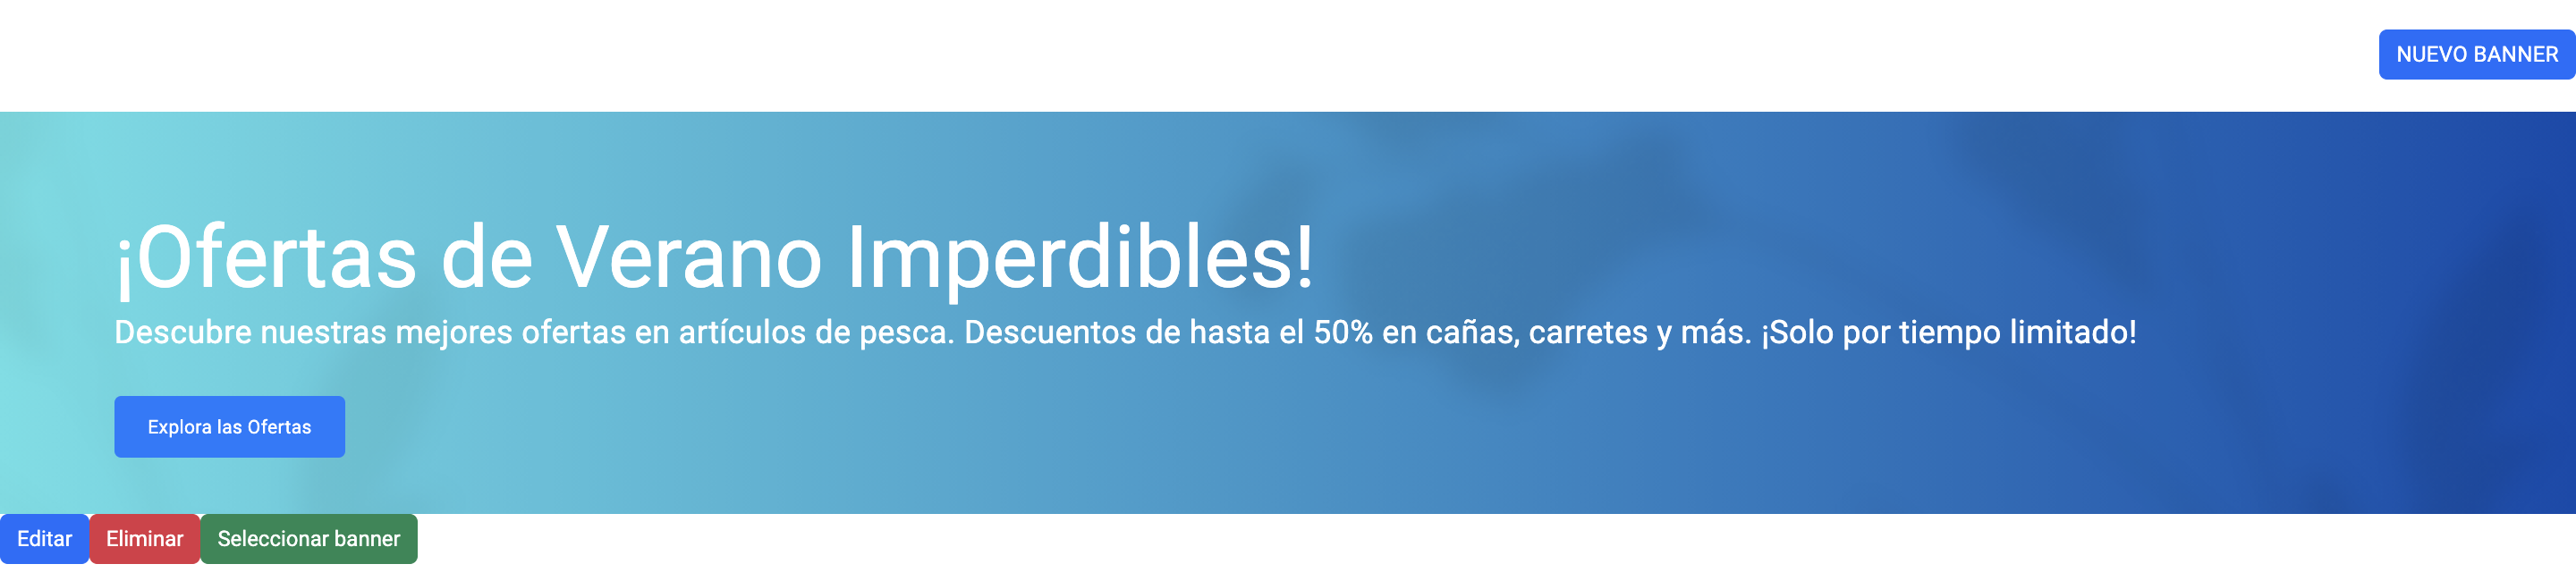
\includegraphics[scale=0.35]{./Images/vistaAdminBanner.png}
\caption{Gestión del banner informativo} Fuente: Elaboración propia.

\label{fig:fig1}

\end{center}
\end{figure}

El segundo módulo corresponde al carrusel de productos más vendidos, pero en realidad, el administrador tiene la libertad de seleccionar manualmente los productos que desea que aparezcan en este carrusel. El límite es de seis productos, y si se intenta seleccionar más, el sistema no lo permite y se muestra un mensaje de advertencia para alertar al administrador de que ha alcanzado el máximo permitido.

\begin{figure}[H]
\begin{center}
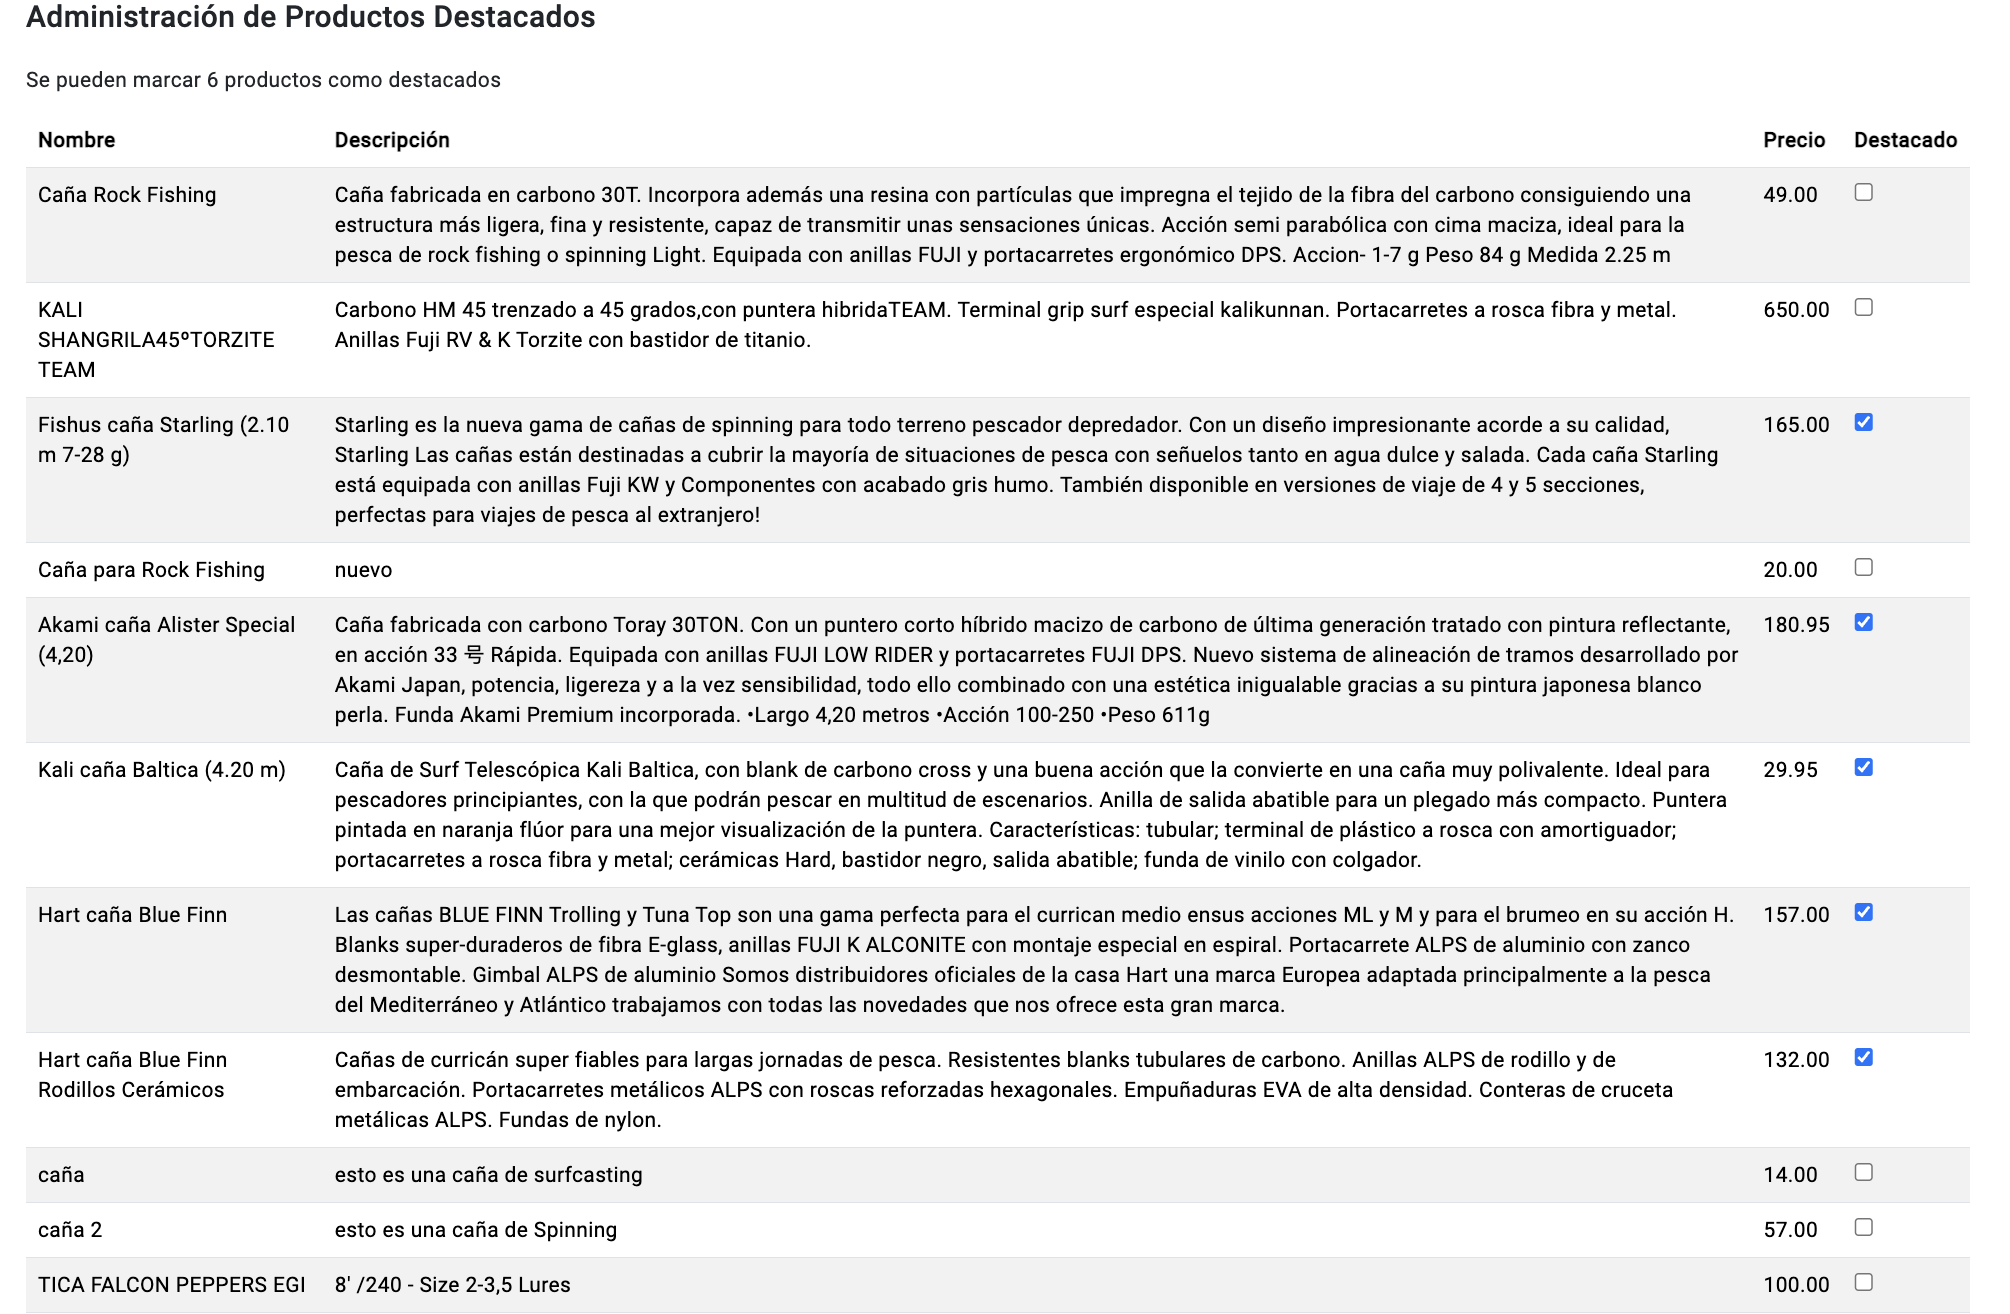
\includegraphics[scale=0.50]{./Images/vistaAdminCarrusel.png}
\caption{Gestión del carrusel de productos} Fuente: Elaboración propia.

\label{fig:fig1}

\end{center}
\end{figure}

El tercer módulo corresponde a las cards de novedades, ofertas y liquidaciones. Cada una de estas tarjetas redirige a una página específica. La tarjeta de novedades lleva a la página de productos marcados como novedades, los cuales se gestionan desde la sección de productos, donde los productos pueden ser marcados o desmarcados como novedades según la decisión del administrador. De manera similar, la tarjeta de liquidaciones lleva a la página de productos en liquidación, y estos también pueden ser marcados o desmarcados como productos en liquidación desde la gestión de productos.

\vspace{0.5cm}

En el caso de la tarjeta de ofertas, esta redirige a la página de productos que tienen precios con descuento. Los productos que se muestran aquí son aquellos que el administrador ha configurado con algún tipo de descuento en su precio.

\begin{figure}[H]
\begin{center}
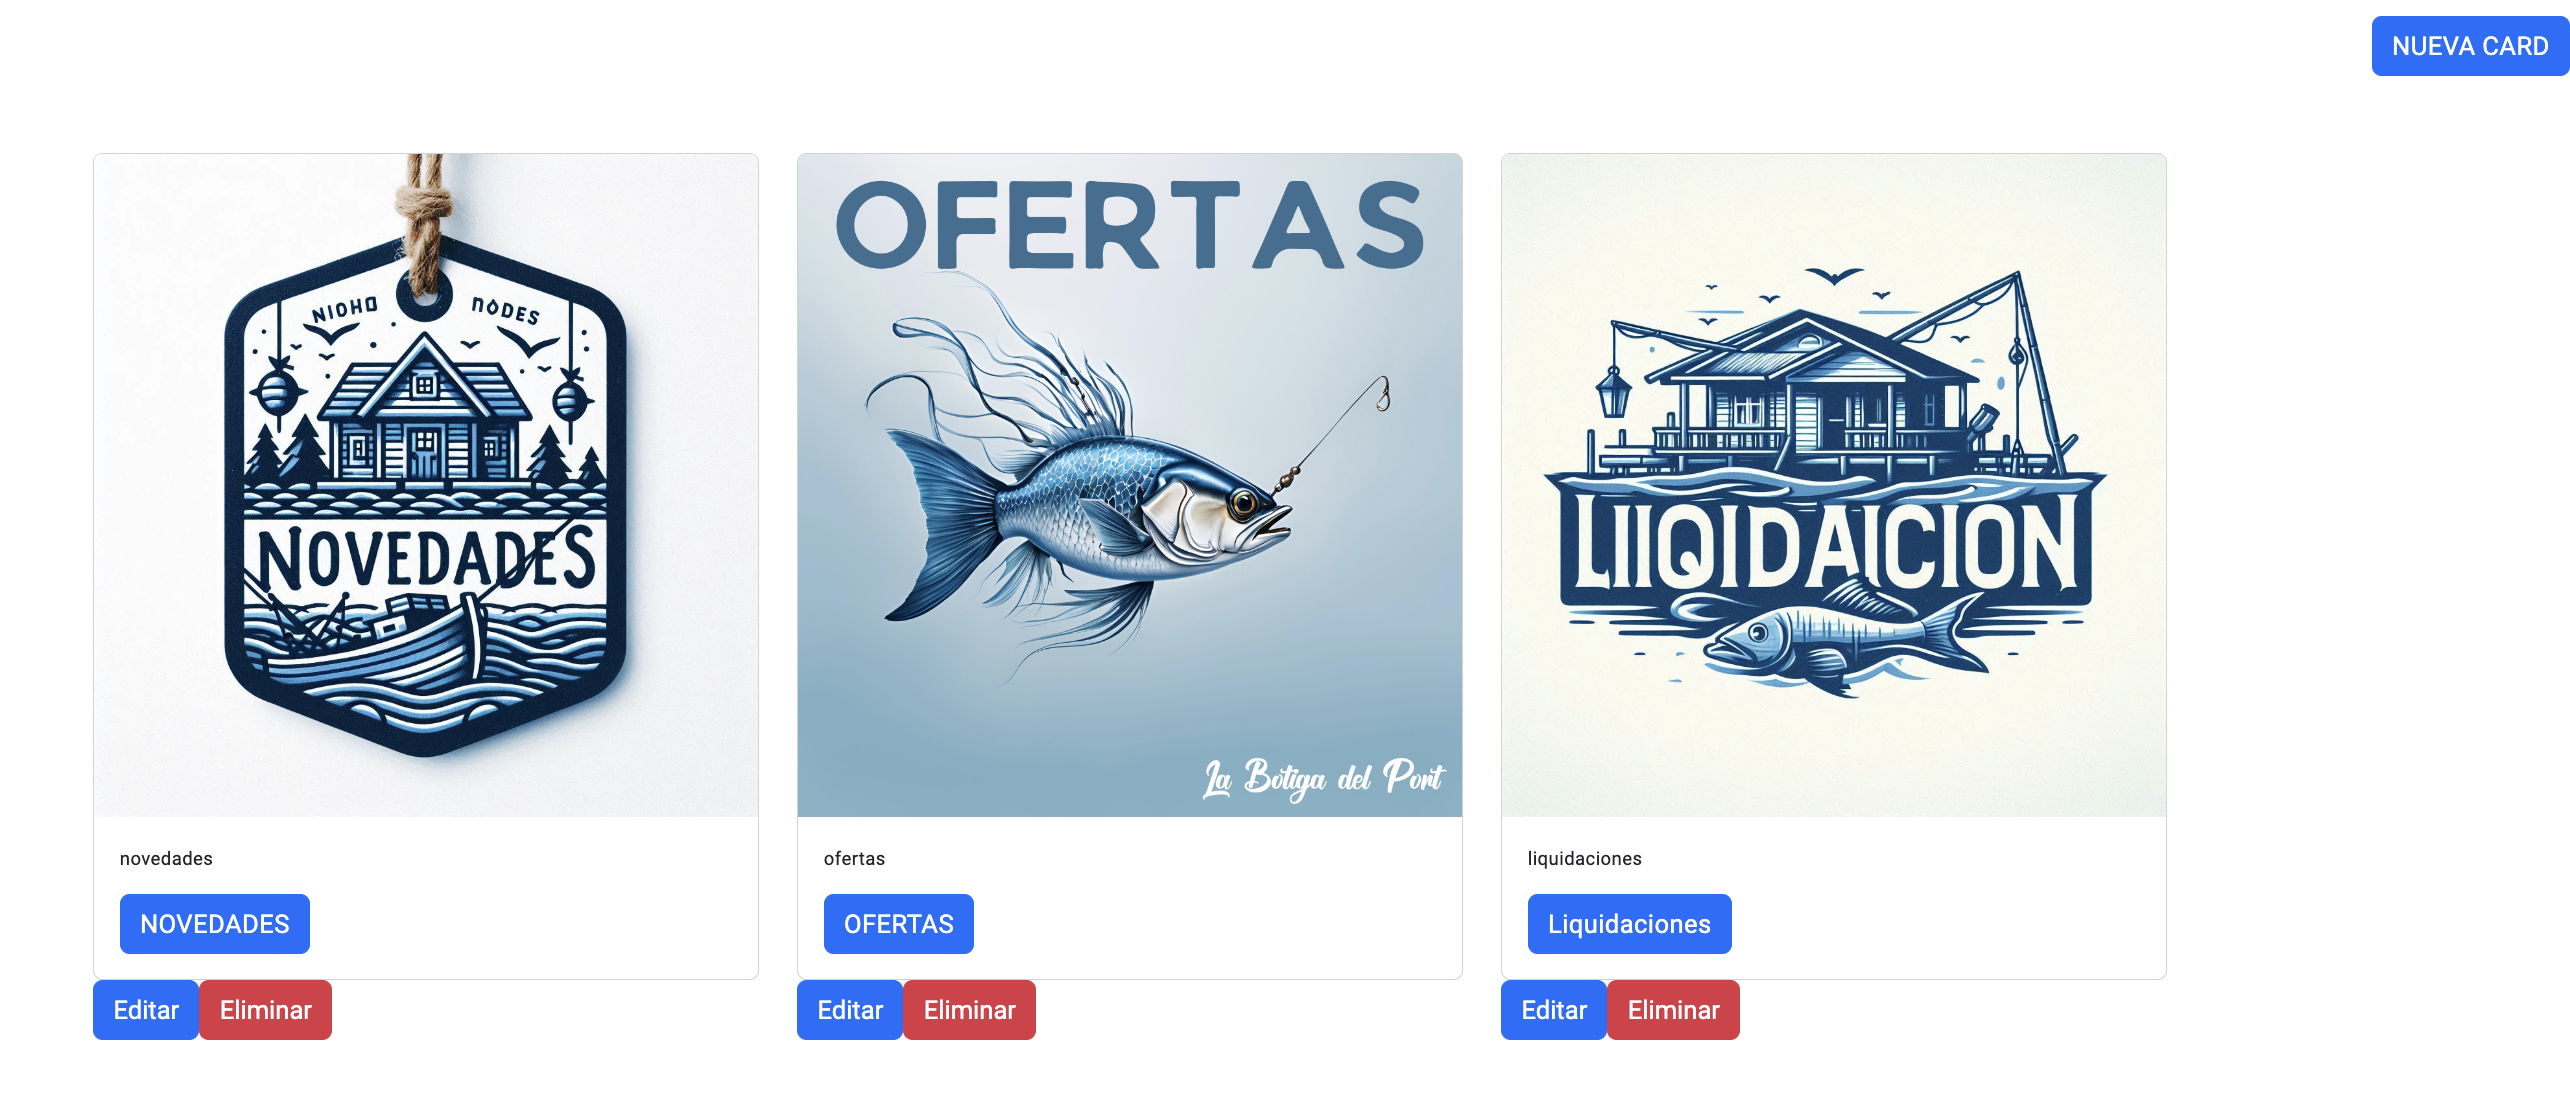
\includegraphics[scale=0.35]{./Images/vistaAdminCards.png}
\caption{Gestión de tarjetas} Fuente: Elaboración propia.

\label{fig:fig1}

\end{center}
\end{figure}

\subsubsection{Códigos de descuento}\label{subsec5.1.2.4}
En esta vista, el administrador puede visualizar todos los códigos de descuento creados hasta el momento. Para cada código, se muestra información clave como el nombre del código, el porcentaje de descuento aplicado, la fecha de inicio y la fecha de finalización del descuento. Además, junto a cada código se incluye una etiqueta que indica si el código está "activo" o si ha pasado su fecha de validez. Junto a estos datos, el administrador dispone de opciones para editar o eliminar cualquier código de descuento existente.

\vspace{0.5cm}

En la parte superior de la vista, se encuentra un botón para crear un nuevo código de descuento. Al seleccionarlo, el administrador deberá completar un formulario que solicita la misma información que se muestra en la lista, es decir, nombre del código, porcentaje de descuentoy fechas de inicio y fin.

\begin{figure}[H]
\begin{center}
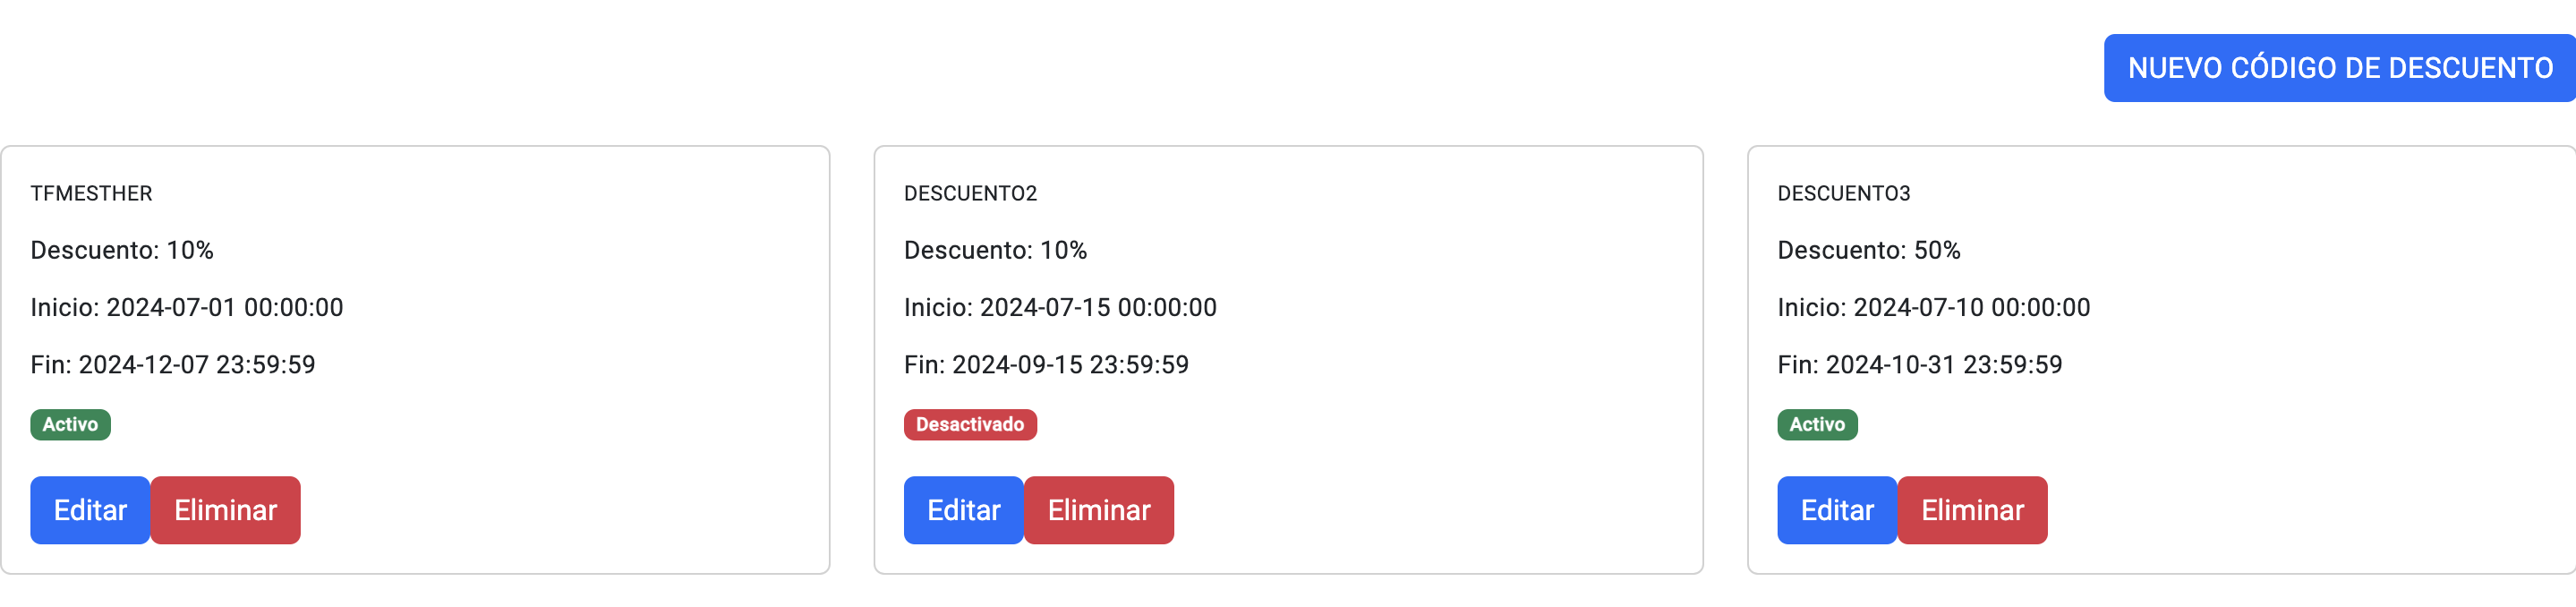
\includegraphics[scale=0.3]{./Images/vistaAdminCodigo.png}
\caption{Vista Códigos de descuento} Fuente: Elaboración propia.

\label{fig:fig2}

\end{center}
\end{figure}

\subsection{Ubicación}\label{subsec5.1.3}

En esta sección, se presenta la vista de la ubicación de La Botiga del Port a través de un mapa interactivo. Esta visualización ha sido posible gracias a la integración de OpenStreetMap, una plataforma de mapeo colaborativa y de código abierto que permite acceder a mapas detallados y actualizados. Los usuarios pueden explorar la ubicación exacta del establecimiento, facilitando su visita y mejorando la experiencia del cliente.

\begin{figure}[H]
\begin{center}
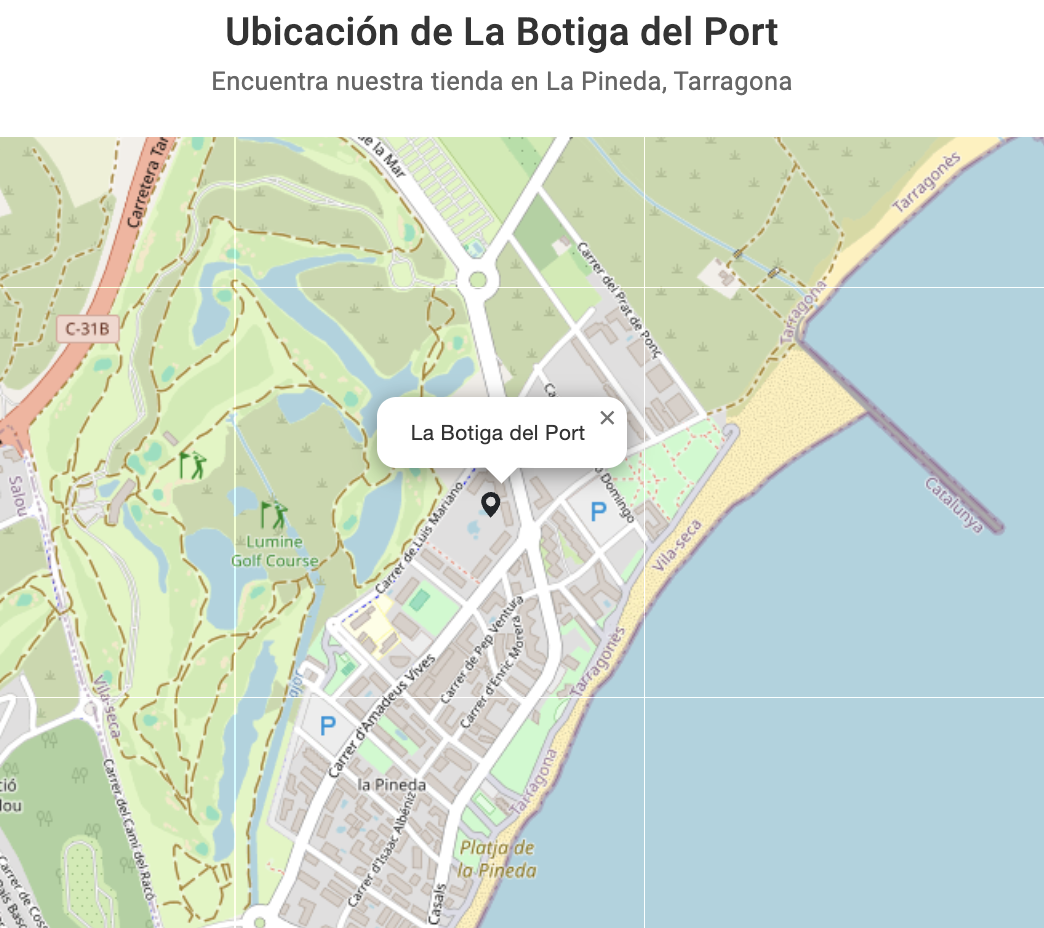
\includegraphics[scale=0.5]{./Images/ubicacion.png}
\caption{Vista de la ubicación} Fuente: Elaboración propia.

\label{fig:fig2}

\end{center}
\end{figure}

\subsection{Navegación en desktop y mobile}\label{subsec5.1.4}
Las vistas de navegación en desktop y mobile están diseñadas de manera diferente para adaptarse a cada tipo de dispositivo, garantizando una experiencia de usuario fluida y optimizada. Mientras que en la versión de escritorio la información se presenta de forma más amplia y accesible en todo momento, en la versión móvil se prioriza la simplicidad y la accesibilidad a través de menús desplegables.

\vspace{0.5cm}

En la versión de escritorio, la navegación se estructura en un header que contiene varios elementos clave. A la izquierda se encuentra el logo de la página, seguido de un buscador central para facilitar la búsqueda rápida de productos. A la derecha se incluyen los botones de login para acceder a la cuenta y el carrito, donde los usuarios pueden visualizar los productos seleccionados. Justo debajo del header, se muestra una barra de navegación con las diferentes categorías de productos. Al hacer clic en una categoría, se despliegan las subcategorías correspondientes, permitiendo una navegación rápida y organizada a través del catálogo.

\begin{figure}[H]
\begin{center}
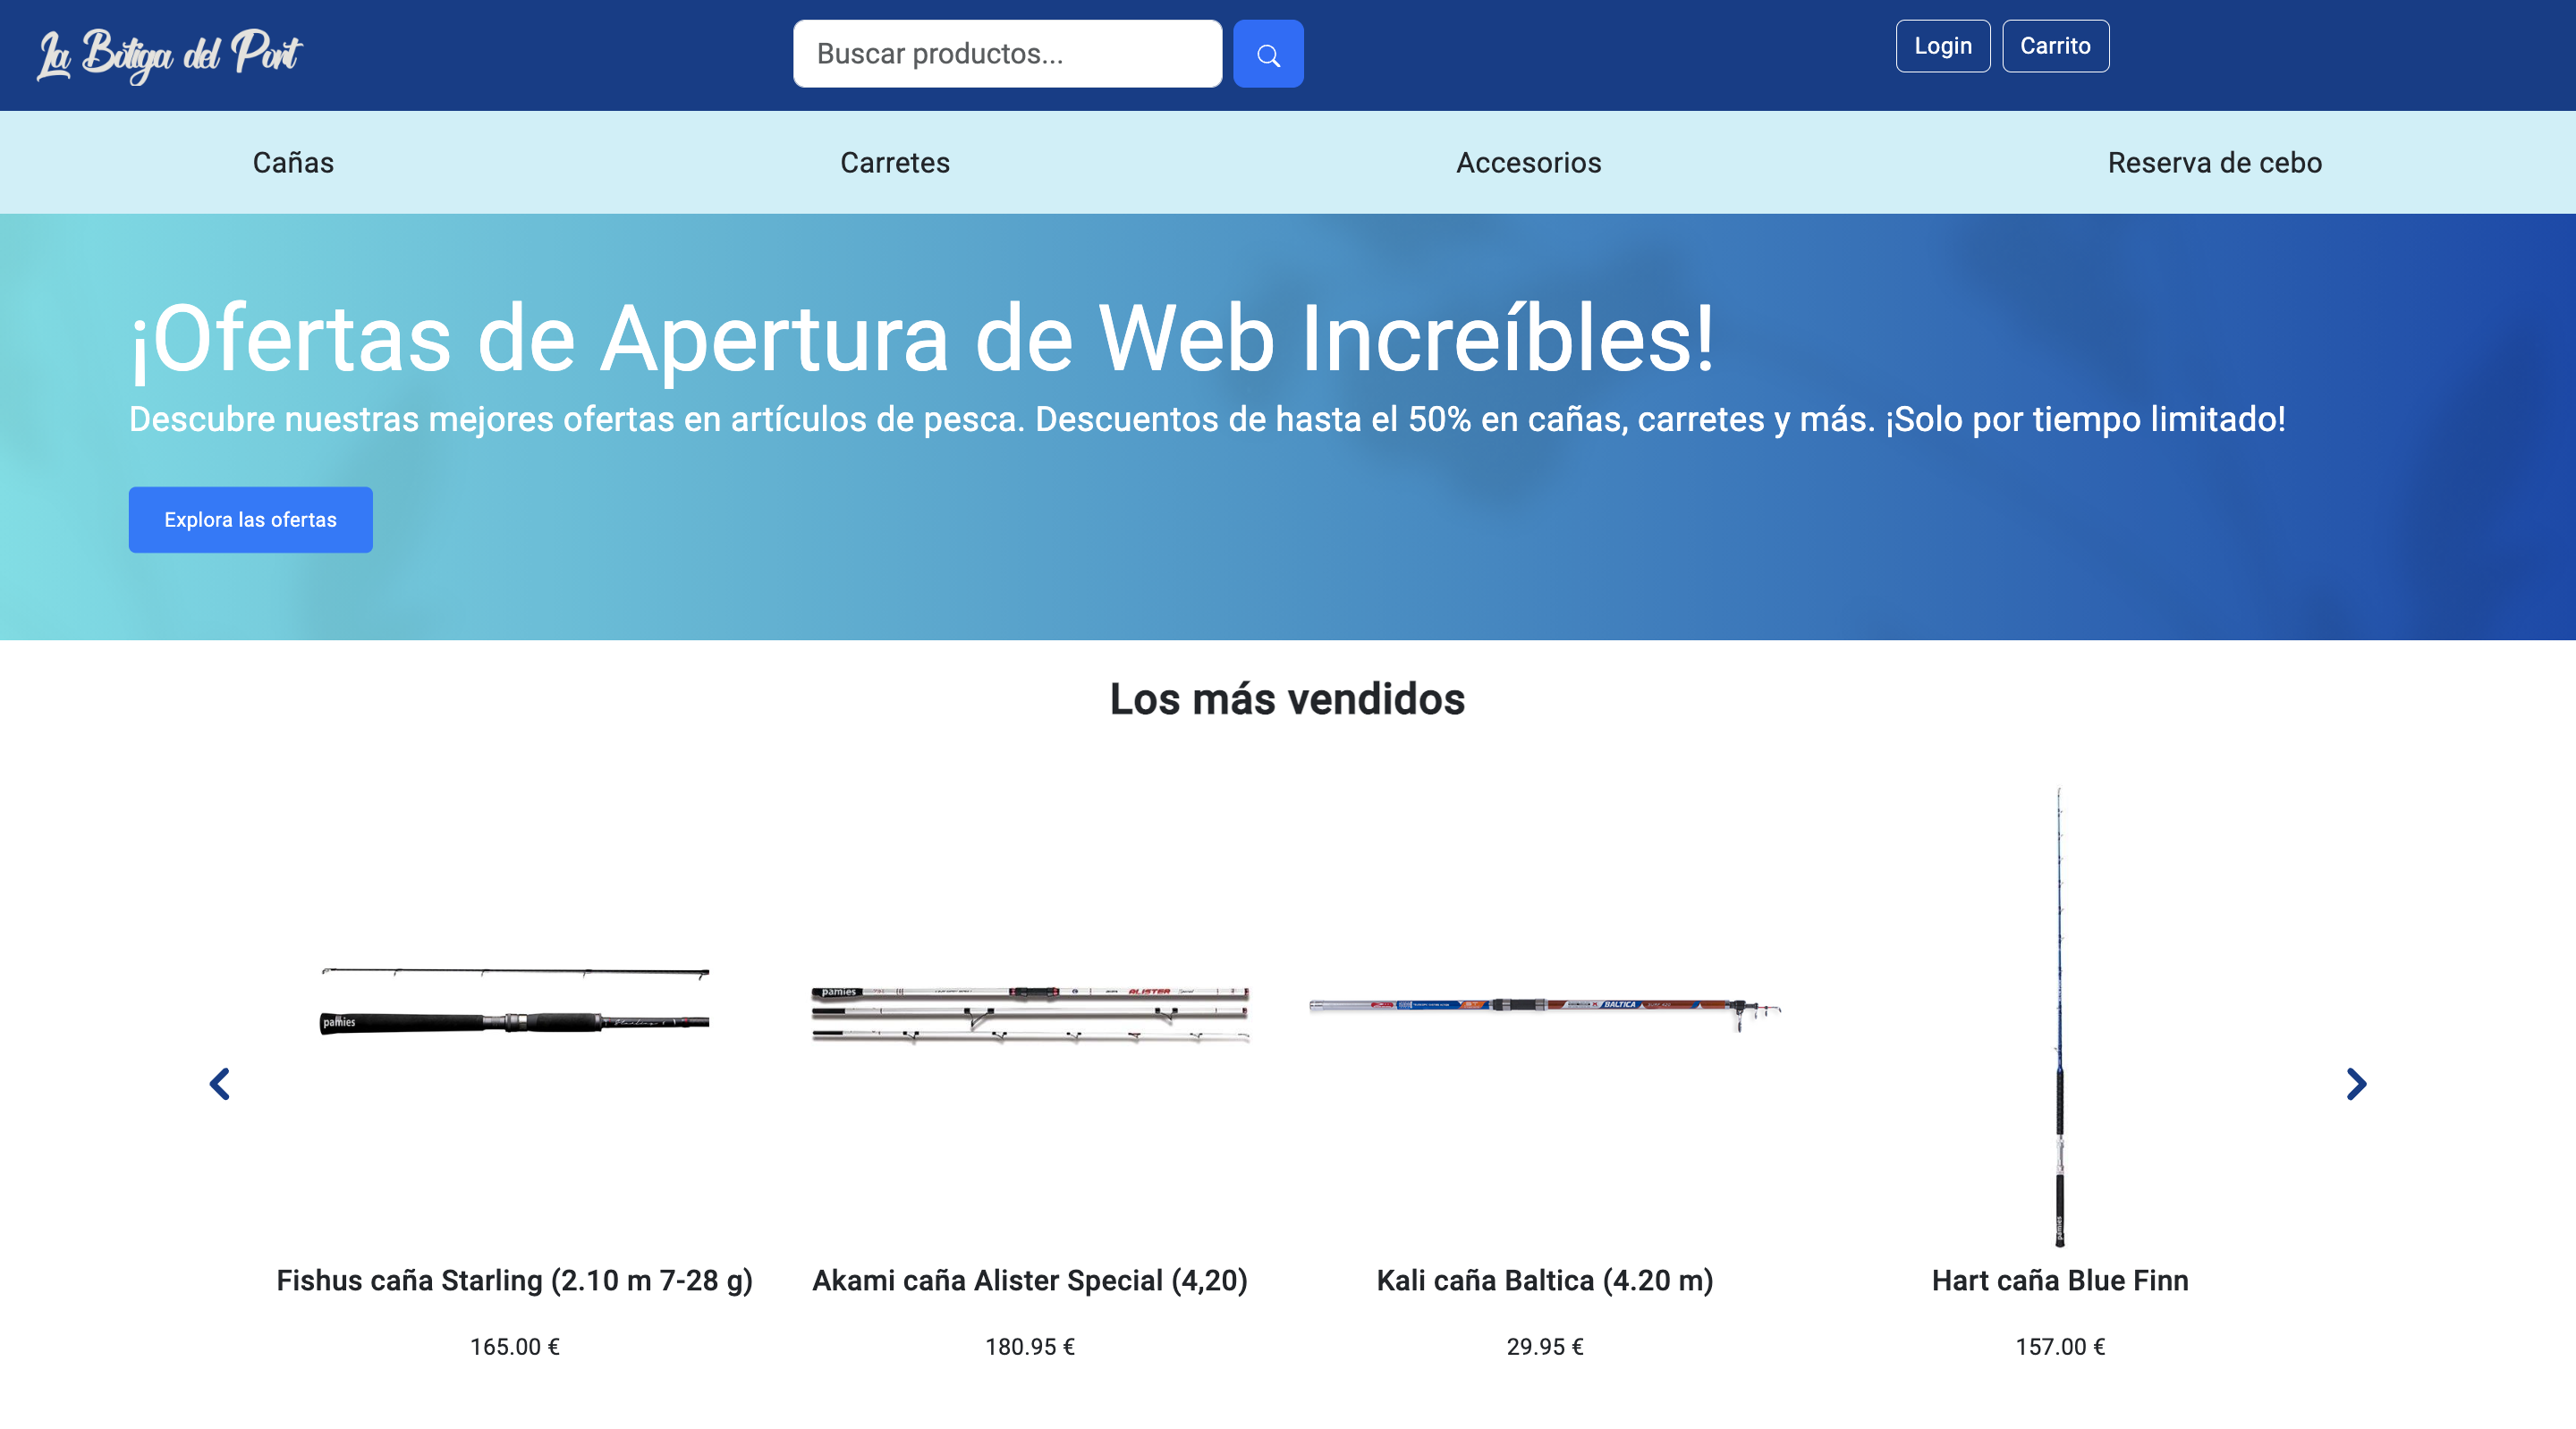
\includegraphics[scale=0.3]{./Images/vistaDesktop.png}
\caption{Vista general en desktop} Fuente: Elaboración propia.

\label{fig:fig2}

\end{center}
\end{figure}

En dispositivos móviles, la navegación está optimizada para pantallas más pequeñas. En la parte superior, solo se muestran el logo y un icono de menú hamburguesa que, al abrirse, despliega un menú lateral. En este menú, el usuario puede acceder al buscador, a los botones de login y carrito, y visualizar todas las categorías de productos. Al seleccionar una categoría, se despliegan las subcategorías relacionadas, permitiendo una navegación clara y eficiente en dispositivos móviles.

\begin{figure}[H]
\begin{center}
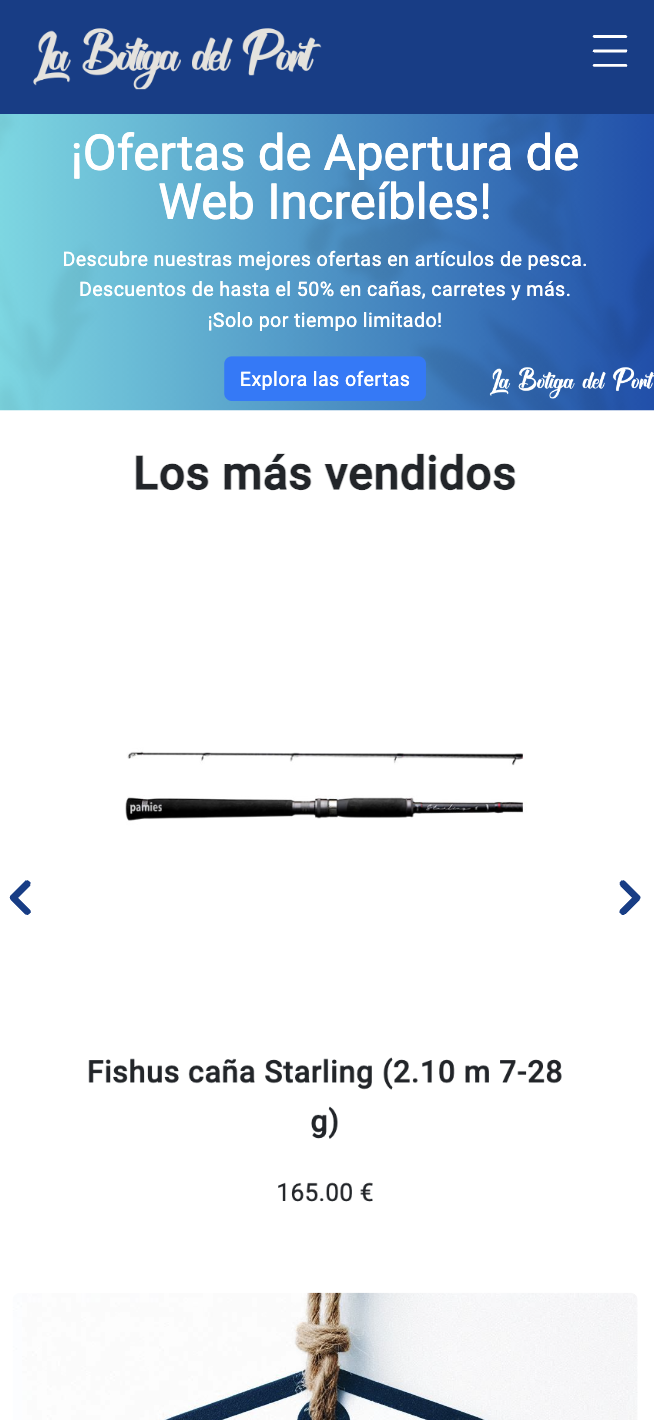
\includegraphics[scale=0.35]{./Images/vistaMobile.png}
\caption{Vista general en mobile} Fuente: Elaboración propia.

\label{fig:fig2}

\end{center}
\end{figure}

\begin{figure}[H]
\begin{center}
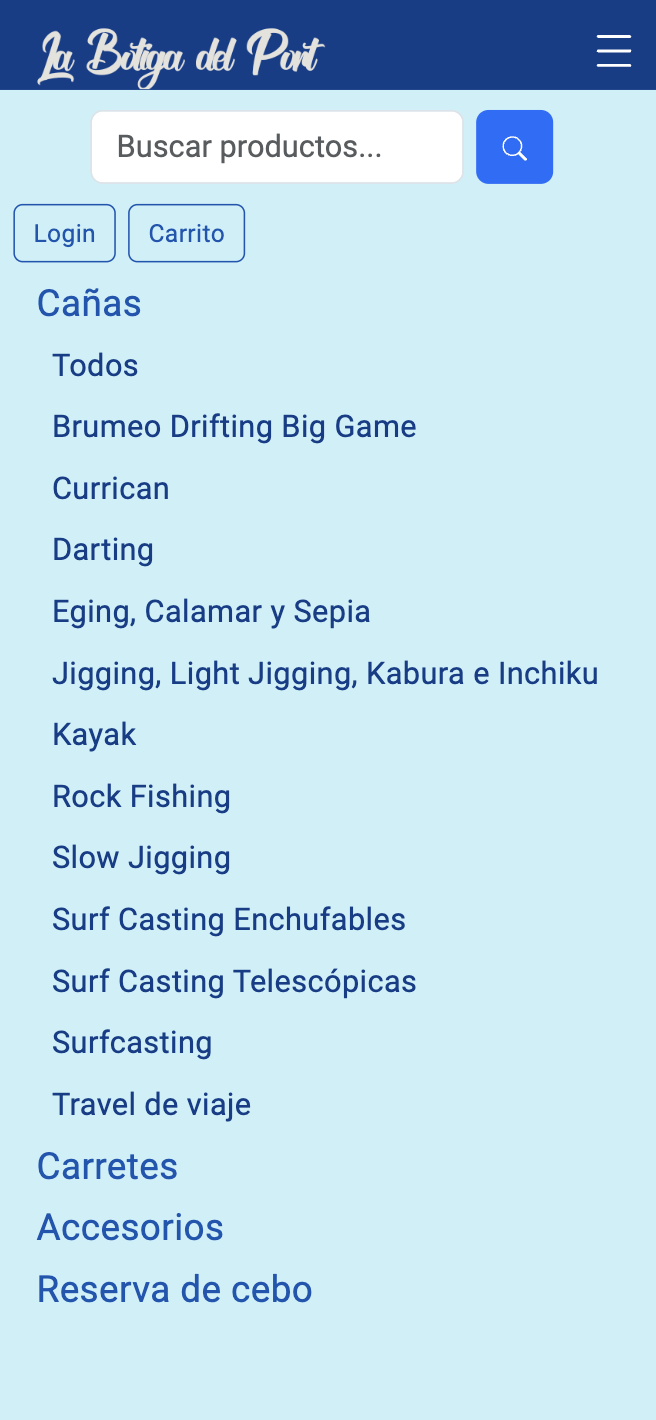
\includegraphics[scale=0.35]{./Images/vistaMobileOpen.png}
\caption{Vista del menú en mobile} Fuente: Elaboración propia.

\label{fig:fig2}

\end{center}
\end{figure}

\section{Uso de la aplicación}\label{sec:apartado}

El uso de la aplicación y las funcionalidades que esta ofrece están directamente basados en los requisitos funcionales establecidos al comienzo del proyecto. Estas funcionalidades han sido diseñadas para garantizar que la aplicación cumpla con los objetivos planteados y proporcione una experiencia de usuario eficaz y coherente.

\subsection{Login y registro de usuario}\label{subsec5.2.1}
    
El login y el registro son funciones fundamentales que permiten a los usuarios interactuar con la aplicación de manera segura y personalizada. El proceso de registro permite la creación de un perfil único para cada usuario, lo que les da acceso a funciones avanzadas como realizar pedidos, reservar cebo y gestionar sus datos. Una vez registrados, los usuarios pueden acceder a su cuenta a través de la funcionalidad de login, la cual asegura que solo aquellos con credenciales válidas puedan acceder a estas funciones específicas. Esto garantiza un control adecuado sobre el acceso y proporciona una experiencia de usuario segura y eficiente dentro de la aplicación.

\vspace{0.5cm}

Adicionalmente, cuando un usuario inicia sesión con credenciales de administrador, la aplicación presenta una vista diferente diseñada específicamente para la gestión administrativa. Esta vista del administrador permite al usuario gestionar diversos aspectos críticos de la aplicación, como productos, pedidos y reservas de cebo. La interfaz administrativa proporciona herramientas para controlar y modificar elementos visuales, gestionar inventarios, y supervisar el estado de las reservas y pedidos. Esta separación entre vistas asegura que las funciones de administración estén claramente diferenciadas y accesibles solo para los usuarios con permisos adecuados, optimizando así la eficiencia y la seguridad en la gestión de la aplicación.

\subsection{Productos}\label{subsec5.2.2}

La gestión de productos dentro de la aplicación es una funcionalidad clave que permite a los usuarios explorar y seleccionar artículos de manera eficiente. A través de la vista de productos, los usuarios pueden navegar por distintas subcategorías, como cañas, carretes y accesorios, o por características específicas como novedades, ofertas y liquidación. Cada producto está presentado con imágenes representativas, descripciones detalladas, y un precio visible, lo que facilita la toma de decisiones de compra. Además, la aplicación permite a los usuarios seleccionar la cantidad de un producto que desean añadir al carrito, haciendo que el proceso de compra sea sencillo e intuitivo.

\vspace{0.5cm}

Los productos añadidos al carrito pueden ser gestionados desde la vista de carrito, donde los usuarios pueden ver todos los artículos que han seleccionado. En esta vista, es posible modificar la cantidad de cada producto o eliminar artículos según sea necesario. A la derecha, se muestra un resumen con la suma total del precio de los productos en el carrito. Además, se ofrece la opción de añadir un código de descuento; si el código es válido, se aplicará automáticamente el descuento correspondiente. En caso contrario, el sistema informará al usuario si el código es inválido o si ha caducado, proporcionando una experiencia de compra transparente y eficaz.

\vspace{0.5cm}

Una vez que el cliente ha añadido los productos deseados al carrito y aplicado cualquier código de descuento, puede proceder al pago presionando el botón de "Pagar". En ese momento, el sistema genera una confirmación de pedido, que se muestra en pantalla con un resumen de los productos adquiridos, sus cantidades y el precio total. Además, una copia de esta confirmación es enviada automáticamente al correo electrónico del cliente, proporcionando un registro del pedido. Simultáneamente, el administrador de la tienda recibe también una notificación por correo electrónico con los detalles del pedido, permitiendo una preparación rápida y eficiente del mismo.

\vspace{0.5cm}

En la pestaña de perfil de la aplicación, el cliente tiene acceso a una vista completa de todos los pedidos que ha realizado a lo largo del tiempo. En esta sección, el cliente puede revisar los detalles de cada uno de sus pedidos pasados, proporcionando un historial claro y organizado. Además, desde la misma pestaña, el usuario puede gestionar sus datos personales, como el nombre, la dirección de correo y otros detalles relevantes para sus futuras compras.

\vspace{0.5cm}

Para el usuario con credenciales de administrador, la aplicación ofrece funcionalidades adicionales que permiten una gestión completa del catálogo de productos. El administrador pueden editar los detalles de cualquier producto, así como eliminar o añadir nuevos artículos a la tienda. También tienen la capacidad de marcar productos como liquidación o novedad, lo que afecta directamente a cómo estos artículos se muestran en las subcategorías específicas de la aplicación. Si un producto tiene un precio con descuento, automáticamente aparece en la subsección de ofertas, asegurando que los usuarios puedan identificar fácilmente las promociones disponibles.

\vspace{0.5cm}

Además de la gestión de productos, los administradores pueden modificar aspectos visuales clave de la aplicación. Esto incluye la capacidad de editar el banner principal, cambiando su texto, imagen y enlace, lo que permite mantener el contenido de la tienda siempre actualizado y relevante. Los administradores también pueden seleccionar qué seis productos aparecen en el carrusel de la página principal, destacando los artículos que se deseen promover. Asimismo, el adminsitrador tienen la posibilidad de gestionar los códigos de descuento, pudiendo añadir nuevos, modificar su nombre o la fecha en que están vigentes, y eliminar aquellos que ya no son necesarios. Estas herramientas de personalización aseguran que la tienda pueda adaptarse rápidamente a nuevas campañas de marketing o promociones, manteniendo una experiencia de usuario dinámica y atractiva.


\subsection{Reserva de Cebo}\label{subsec5.2.3}

La funcionalidad de reserva de cebo dentro de la aplicación ofrece a los clientes una forma sencilla y eficiente de seleccionar y reservar cebo para recoger en tienda en una fecha posterior. En la subpágina dedicada a la reserva de cebo, se muestran todos los productos disponibles de esta categoría, cada uno acompañado de su imagen representativa, nombre y precio, facilitando así la exploración de las opciones disponibles. Junto a cada producto, el cliente encontrará botones para seleccionar la cantidad de cebo que desea reservar.

\vspace{0.5cm}

En la parte superior de esta vista, se ofrece un campo de entrada tipo calendario, que permite al cliente seleccionar la fecha en la que desea recoger su reserva. Esta fecha debe ser siempre posterior al día actual, lo que garantiza que el administrador disponga del tiempo necesario para preparar el pedido. Una vez seleccionados los productos y la fecha de recogida, el cliente puede proceder a realizar la reserva mediante el botón de "Reservar cebo". 

\vspace{0.5cm}

Para continuar con la reserva, el cliente debe estar registrado y haber iniciado sesión. Si no lo ha hecho, la aplicación redirigirá al cliente a la página de inicio de sesión, donde podrá autenticarse o crear una cuenta si aún no tiene una. Una vez autenticado, el cliente será redirigido de nuevo a la página de resumen de su reserva, donde podrá revisar y modificar los productos seleccionados, la cantidad de cada uno y la fecha de recogida. Cuando esté satisfecho con los detalles de su reserva, podrá confirmarla.

\vspace{0.5cm}

Tras la confirmación de la reserva, el cliente verá una pantalla de confirmación y, además, recibirá un correo electrónico con los detalles de la reserva, para tener un registro permanente de la misma. De manera simultánea, el administrador de la tienda también recibirá un correo electrónico con los detalles de la reserva, lo que le permitirá preparar con antelación los pedidos que se recogerán en el futuro.

\vspace{0.5cm}

En la interfaz de administración, el sistema ofrece una vista completa de todas las reservas de cebo realizadas por los clientes. El administrador puede visualizar cada reserva con sus detalles, como el nombre del cliente, los productos reservados, la cantidad de cada uno y la fecha de recogida. Esta vista incluye filtros que permiten al administrador organizar las reservas según sean pasadas o futuras, o bien buscar reservas específicas por el nombre del cliente. 

\vspace{0.5cm}

Cuando un cliente acude a la tienda para recoger su cebo, el administrador puede marcar la reserva como "recogida", lo que facilita el seguimiento de las reservas completadas y garantiza un control eficaz sobre los pedidos. De este modo, la funcionalidad asegura que tanto el cliente como el administrador puedan gestionar el proceso de reserva y recogida de forma rápida, clara y eficiente, proporcionando una experiencia de usuario fluida y un control administrativo preciso.
\section{APIs utilizadas}\label{sec:apartado}

El desarrollo de la aplicación ha requerido la implementación de diversas APIs que permiten la comunicación entre el backend, desarrollado en Laravel, y el frontend, construido con Angular. Estas APIs son fundamentales para gestionar las operaciones de la aplicación, garantizando el correcto funcionamiento de la web y la gestión de la base de datos de manera segura y eficiente. A continuación, se describe en detalle el conjunto de APIs implementadas.

\subsection{Login y registro de usuario}\label{subsec5.3.1}

Para manejar las operaciones relacionadas con la creación y autenticación de usuarios, se han desarrollado cuatro APIs específicas. Estas APIs son fundamentales para asegurar que los usuarios puedan registrarse, iniciar sesión, y que los administradores puedan gestionar las cuentas de manera efectiva. A continuación, se presenta una descripción detallada de cada una de estas APIs.

\begin{itemize}
    \item \textbf{Obtener todos los usuarios:} Esta API permite obtener un listado completo de los usuarios registrados en la aplicación. Es utilizada principalmente por los administradores para supervisar y gestionar las cuentas de usuario. Al invocar este endpoint, se devuelve un JSON con la información básica de cada usuario, excluyendo datos sensibles como contraseñas. Este endpoint es clave para mantener una visión general del estado de la base de datos de usuarios.
    
    \item \textbf{Registro de usuario:} La API de registro es responsable de crear nuevas cuentas de usuario. Recibe datos como correo electrónico, contraseña, y otros detalles relevantes, los valida y, tras comprobar que el correo electrónico no esté en uso, encripta la contraseña y almacena la información en la base de datos. Si el registro es exitoso, la API responde con un mensaje de confirmación junto con los detalles del nuevo usuario, asegurando así un proceso de registro fluido y seguro.
    
    \item \textbf{Login de usuario:} Esta API gestiona la autenticación de los usuarios que intentan acceder a la aplicación. Tras recibir el correo electrónico y la contraseña, la API verifica las credenciales contra las almacenadas en la base de datos. Si la autenticación es correcta, se genera un token de sesión, que es devuelto al frontend para autenticar futuras solicitudes. En caso de error, la API proporciona un mensaje adecuado para notificar al usuario del problema.

    \item \textbf{Eliminar usuario:} La API de eliminación de usuario permite a los administradores eliminar cuentas de la base de datos de manera permanente. Al ejecutarse correctamente, la API devuelve una confirmación de que el usuario ha sido eliminado, lo que ayuda a mantener la base de datos actualizada y libre de cuentas innecesarias.
    
\end{itemize}

\subsection{Productos y pedidos}\label{subsec5.3.2}

En la gestión de productos y pedidos dentro de la aplicación, se han implementado diversas APIs que permiten tanto a los usuarios como a los administradores interactuar de manera eficiente con el catálogo. Estas APIs son fundamentales para garantizar que la información de los productos esté siempre disponible y sea manejada de manera segura y eficiente. La estructura de estas APIs facilita tanto la experiencia de compra para los usuarios finales como la gestión y administración de los productos por parte del equipo responsable de la tienda. A continuación, se presentan las APIs categorizadas según su uso para el cliente y para el administrador.

\subsubsection{APIs para el cliente}\label{subsec5.3.2.1}
Las APIs orientadas al usuario están diseñadas para proporcionar acceso a la información de los productos de manera rápida y sencilla. Estas permiten a los usuarios navegar por las distintas categorías y subcategorías, visualizar detalles específicos de los productos, acceder a las secciones especiales como ofertas, novedades o productos en liquidación y realizar pedidos.

\begin{itemize}
    \item \textbf{Obtener información de un producto específico:} Esta API de tipo GET permite a los usuarios obtener la información detallada de un producto específico mediante el uso de su ID. Al invocar este endpoint y proporcionar el ID del producto, la API devuelve un JSON con los detalles completos del producto, incluyendo su nombre, descripción, imágenes, precio, y cualquier otra característica relevante. Esta funcionalidad es esencial para la vista de detalle del producto, donde los usuarios pueden explorar toda la información antes de tomar una decisión de compra.
    
    \item \textbf{Obtener productos por categoría con paginación:} Para facilitar la navegación en el catálogo, se ha implementado una API GET que permite obtener productos según su categoría. Esta API recibe como parámetros la categoría deseada, el número de página y la cantidad de elementos por página. La API devuelve un conjunto de productos que pertenecen a la categoría indicada, organizados en la página correspondiente. Este endpoint es crucial para la paginación dentro de la aplicación, garantizando que los usuarios puedan explorar cómodamente todas las opciones disponibles sin sobrecargar la interfaz.
    
    \item \textbf{Obtener productos por categoría y subcategoría con paginación:} Similar a la API anterior, esta API GET se utiliza para obtener productos filtrados tanto por categoría como por subcategoría. Al recibir los parámetros de categoría, subcategoría, número de página y elementos por página, la API devuelve una lista de productos que coinciden con los criterios especificados. Esto es particularmente útil para los usuarios que desean explorar productos dentro de una subcategoría específica, como accesorios dentro de la categoría de cañas.

    \item \textbf{Obtener subcategorías de una categoría:} A través de una petición GET, esta API permite obtener todas las subcategorías que pertenecen a una categoría específica. Al pasar como parámetro la categoría principal, la API devuelve un listado de las subcategorías asociadas, lo que es esencial para construir y visualizar el menú superior de navegación. Este endpoint asegura que los usuarios puedan explorar las diferentes divisiones del catálogo de manera organizada y clara, mejorando la experiencia de navegación en la aplicación.

    \item \textbf{Obtener productos por ofertas, novedades o liquidaciones:} Esta API GET está diseñada para manejar la visualización de productos especiales, como los que están en oferta, son novedades o están en liquidación. Al pasar los parámetros correspondientes, la API devuelve los productos que coinciden con estas características, permitiendo a los usuarios enfocarse en las promociones actuales o en los últimos lanzamientos. Además, esta API soporta la paginación, permitiendo una navegación fluida incluso dentro de estas secciones específicas del catálogo.

    \item \textbf{Obtener todos los productos destacados:} Esta API, mediante una petición GET, devuelve un listado de todos los productos que han sido marcados como "destacados" por el administrador. Los productos destacados se muestran en el carrusel de la página principal, y este endpoint permite al frontend obtener la información necesaria para visualizarlos correctamente. Al llamar a esta API, se envía un JSON con los detalles relevantes de cada producto destacado, como nombre, precio e imagen. Esta funcionalidad es clave para resaltar productos seleccionados en la página de inicio y fomentar su visibilidad entre los usuarios.

    \item \textbf{Crear un nuevo pedido de productos:} A través de una petición POST, esta API permite a los usuarios realizar un pedido de productos. Al invocar el endpoint, se envía un conjunto de datos que incluye el ID del usuario, los productos seleccionados con sus respectivos IDs, cantidades, y el precio total del pedido. Una vez confirmado el pedido, la API devuelve un mensaje de éxito junto con los detalles del pedido, como el número de pedido y el total pagado.
    
    \item \textbf{Obtener detalles de un pedido específico:} Mediante una petición GET, esta API permite a los usuarios acceder a la información detallada de un pedido previamente realizado. Al proporcionar el ID del pedido, la API devuelve un JSON con los datos completos, incluyendo el número de pedido, los productos adquiridos, las cantidades y el precio total. Esta información es útil tanto para el usuario como para el administrador para hacer seguimiento de los pedidos.

    
\end{itemize}

\subsubsection{APIs para el administrador}\label{subsec5.3.2.2}
Las APIs para el administrador están enfocadas en la gestión y administración del catálogo de productos. A través de estas APIs, el administrador puede añadir, editar, eliminar productos, gestionar su visibilidad en las diferentes secciones de la tienda (ofertas, novedades, liquidación), y controlar aspectos visuales clave como el banner y el carrusel de productos.

\begin{itemize}

    \item \textbf{Crear un nuevo producto:} Mediante una petición POST, esta API permite al administrador agregar un nuevo producto al catálogo. Al invocar este endpoint, se deben enviar los detalles completos del producto. La API valida los datos proporcionados, crea un nuevo registro en la base de datos y responde con un mensaje de confirmación junto con los detalles del producto recién creado. Esta funcionalidad es esencial para expandir el catálogo de productos, permitiendo al administrador introducir nuevos artículos y mantener el inventario actualizado.
    
    \item \textbf{Eliminar un producto:} Esta API permite al administrador eliminar un producto del catálogo mediante una petición DELETE. Al invocar este endpoint, se debe proporcionar el ID del producto que se desea eliminar. Una vez realizada la solicitud, la API elimina el producto de la base de datos y responde con un mensaje de confirmación, asegurando que el producto ha sido removido exitosamente. Esta funcionalidad es clave para mantener el catálogo actualizado y eliminar productos obsoletos o fuera de inventario.
    
    \item \textbf{Editar un producto:} Para modificar los detalles de un producto, se ha implementado una API disponible tanto para peticiones PUT como PATCH, lo que otorga flexibilidad al administrador. En el caso de PUT, el administrador debe proporcionar todos los campos del producto que se desean actualizar, reemplazando la información anterior por completo. Por otro lado, PATCH permite modificar campos específicos, como el precio o la descripción, sin alterar el resto de la información del producto. Ambas operaciones requieren el ID del producto y responden con un mensaje confirmando que los cambios han sido aplicados con éxito.
    
    \item \textbf{Marcar o desmarcar productos como novedades, liquidación o destacados:} Esta API, accesible mediante una petición PUT, permite al administrador cambiar el estado de un producto para clasificarlo como novedad, liquidación o destacado en el carrusel de la página de inicio. Pasando el ID del producto y el estado correspondiente, el administrador puede marcar o desmarcar el producto en estas categorías especiales. Esto facilita la gestión del inventario, destacando productos estratégicos y asegurando que el catálogo refleja las promociones y ofertas actuales de la tienda.

    \item \textbf{Obtener todos los pedidos:} Esta API GET permite al administrador obtener un listado completo de todos los pedidos de productos realizados por los clientes. La respuesta incluye los detalles de cada pedido, la información del cliente, los productos comprados, las cantidades y el precio total.

    
\end{itemize}

\subsection{Reserva de cebo}\label{subsec5.3.3}

Para gestionar de manera eficiente la funcionalidad de reserva de cebo en la aplicación, se han implementado diversas APIs que permiten tanto a los usuarios como a los administradores realizar y administrar reservas de manera segura y rápida. Estas APIs aseguran que los clientes puedan gestionar sus reservas de forma eficaz, mientras que los administradores tienen acceso a herramientas para controlar y supervisar el proceso de recogida. A continuación, se presentan las APIs categorizadas según su uso para el cliente y para el administrador.

\vspace{0.5cm}

\subsubsection{APIs para el cliente}\label{subsec5.3.3.1}

Las APIs orientadas al cliente permiten gestionar todos los aspectos de la reserva de cebo, desde la selección del producto hasta la confirmación de la reserva. Estas APIs aseguran que los usuarios puedan interactuar con la aplicación de forma fluida y acceder a la información necesaria para completar sus reservas.

\begin{itemize}

     \item \textbf{Obtener todos los productos de la categoría de cebo:} Similar a la funcionalidad para productos generales, esta API GET permite a los clientes obtener un listado de todos los productos de la categoría cebo organizados por páginas. La API recibe como parámetros el número de página y la cantidad de productos por página, devolviendo un conjunto de resultados que facilita la navegación por las diferentes opciones disponibles.
     
    \item \textbf{Crear una nueva reserva de cebo:} Mediante una petición POST, esta API permite a los usuarios realizar una reserva de cebo. Al invocar el endpoint, se envía un conjunto de datos que incluye la fecha actual (automáticamente generada por la aplicación), la fecha de recogida seleccionada por el cliente, el ID del usuario, el ID del producto (cebo) y las unidades reservadas de cada producto. Una vez confirmada la reserva, la API devuelve un mensaje de éxito junto con los detalles de la misma.
    
    \item \textbf{Obtener detalles de una reserva específica:} A través de una petición GET, esta API permite a los usuarios obtener la información detallada de una reserva previamente realizada. Al proporcionar el ID de la reserva, la API devuelve un JSON con los detalles completos de la misma, incluyendo el estado de la reserva, los productos reservados, la fecha de recogida y cualquier otra información relevante para el cliente.


\end{itemize}

\vspace{0.5cm}

\subsubsection{APIs para el administrador}\label{subsec5.3.3.2}

Las APIs orientadas al administrador están diseñadas para gestionar de manera eficaz todas las reservas de cebo, permitiendo tanto el filtrado de reservas según su estado como la actualización de su estado una vez que el cliente haya recogido el pedido.

\begin{itemize}

    \item \textbf{Obtener todas las reservas:} Esta API GET permite al administrador obtener un listado completo de todas las reservas de cebo realizadas por los clientes. La respuesta incluye los detalles de cada reserva, como el nombre del cliente, los productos reservados, la fecha de recogida y el estado actual de la reserva.
    
    \item \textbf{Obtener reservas pasadas y futuras:} A través de una petición GET, estas APIs permiten al administrador filtrar las reservas en función de la fecha actual. Al recibir los parámetros 'futuras' o 'pasadas', la API devuelve un listado de las reservas que aún no han sido recogidas (futuras) o las que ya han sido completadas (pasadas), facilitando así la organización y planificación de los pedidos en la tienda.
    
    \item \textbf{Obtener reservas de un usuario específico:} Esta API GET permite obtener todas las reservas asociadas a un cliente específico, identificándolo por su ID de usuario. Es particularmente útil para que el administrador pueda atender consultas o reclamaciones de los clientes de forma personalizada, facilitando la búsqueda rápida de las reservas asociadas a un cliente concreto.
    
    \item \textbf{Borrar una reserva:} Mediante una petición DELETE, esta API permite al administrador eliminar una reserva de la base de datos. Al invocar este endpoint, se debe proporcionar el ID de la reserva que se desea eliminar. Tras confirmar la eliminación, la API responde con un mensaje de éxito, asegurando que la reserva ha sido eliminada correctamente.
    
    \item \textbf{Marcar una reserva como recogida:} Esta API PUT permite al administrador actualizar el estado de una reserva una vez que el cliente haya recogido el cebo. Al proporcionar el ID de la reserva, la API actualiza su estado a 'recogida', lo que facilita el control de las reservas completadas y asegura que el sistema mantiene un registro preciso de todas las interacciones del cliente.

\end{itemize}

\vspace{0.5cm}

En este apartado se describen las principales APIs desarrolladas para la aplicación, detallando sus métodos, endpoints y funcionalidades. Para una visualización más detallada de las pruebas realizadas y la estructura completa de las APIs, se puede consultar la colección de Postman exportada, que se incluye en el \textcolor{naranja}{Anexo II: APIs utilizadas}

\vspace{0.5cm}

\section{Aspectos destacables de programación}\label{sec:apartado}

El desarrollo de la aplicación ha implicado la implementación de diversas funcionalidades clave que destacan tanto por su complejidad como por las soluciones adoptadas para garantizar un rendimiento óptimo y una experiencia de usuario segura y fluida. A continuación, se detallan algunos de los aspectos más relevantes en la programación.

\subsection{Login y registro de usuario}\label{subsec5.4.1}

El proceso de registro y autenticación de usuarios ha sido implementado con especial atención a la seguridad, la validación de datos y la eficiencia en la comunicación entre el backend y el frontend. A continuación, se describen los aspectos más destacados de esta implementación:

\begin{itemize}
    \item \textbf{Validación de Datos y Reglas Personalizadas en Laravel} 

    \begin{itemize}
        \item En el controlador UsuarioController, se implementan diversas reglas de validación para garantizar la integridad de los datos introducidos por los usuarios al registrarse. Se utilizan tanto reglas estándar de Laravel como reglas personalizadas, como ValidarDNI, ValidarTelefono, y ValidarPassword. Estas reglas se encargan de verificar que los datos cumplen con los requisitos de formato y seguridad antes de proceder a su almacenamiento.
        
        
        \item Además de la validación, se implementa el hash de la contraseña mediante Hash::make() antes de almacenarla en la base de datos, asegurando que las contraseñas nunca se guarden en texto plano, lo que refuerza la seguridad de la aplicación.
        
    \end{itemize}

    \vspace{0.5cm}
    
    \item \textbf{Gestión de Autenticación y Tokenización} 

    \begin{itemize}
        \item Durante el proceso de login, el controlador valida las credenciales proporcionadas y, si son correctas, genera un token de acceso personal utilizando el método createToken() del modelo Usuario. Este token es enviado al frontend, donde se almacena en el localStorage para ser utilizado en futuras solicitudes autenticadas. Esta técnica de tokenización asegura que las sesiones del usuario sean seguras y manejables desde el frontend.
        
        
        \item El manejo de errores es otra característica destacable. Si el usuario no es encontrado o si la contraseña es incorrecta, se devuelven respuestas HTTP específicas (404) con mensajes adecuados, lo que permite al frontend manejar estos errores de manera efectiva.
        
    \end{itemize}

    \vspace{0.5cm}
    
    \item \textbf{Frontend con Angular: Manejo de Estado y Almacenamiento en Local Storage} 

        \begin{itemize}
        \item En el componente LoginComponent de Angular, se realiza un cuidadoso manejo del estado del usuario y de la gestión de la autenticación. Cuando un usuario inicia sesión correctamente, el token y la información del usuario se almacenan en el localStorage, lo que permite mantener la sesión activa incluso después de que el usuario cierre el navegador o recargue la página.
        
        
        \item La visibilidad de la contraseña es otra funcionalidad implementada en el frontend, permitiendo al usuario alternar entre ver y ocultar su contraseña mediante un simple botón. Esto mejora la experiencia de usuario sin comprometer la seguridad.

        \item Además, se implementa una validación asíncrona del correo electrónico en el frontend para verificar que el formato sea correcto y que el correo esté registrado en el sistema antes de enviar las credenciales, lo que añade una capa adicional de robustez a la validación de datos en el cliente.
        
    \end{itemize}

    \vspace{0.5cm}

\end{itemize}

\subsection{Productos}\label{subsec5.4.2}

Los productos es una de las piezas centrales en el funcionamiento de la aplicación, ya que permite la gestión eficiente de todos los artículos disponibles en la plataforma. Para su implementación, se han desarrollado funcionalidades tanto en el backend como en el frontend, garantizando que los usuarios puedan interactuar de manera rápida, segura y eficiente con el catálogo de productos.

\vspace{0.5cm}

Desde el backend, se manejan operaciones como la creación, actualización, eliminación y consulta de productos, así como la categorización, paginación y gestión de descuentos. Estas operaciones han sido diseñadas con especial atención a la robustez del código, la escalabilidad y el manejo adecuado de las imágenes asociadas a cada producto. Asimismo, se han implementado diferentes tipos de productos destacados, como novedades y liquidaciones, para ofrecer una experiencia personalizada a los usuarios.

\vspace{0.5cm}

En el frontend, se abordarán aspectos cruciales como la presentación del catálogo de productos, la navegación por categorías y subcategorías, el uso de filtros para facilitar la búsqueda y la visualización de productos en oferta o destacados. Se ha tenido en cuenta la optimización del rendimiento y la experiencia del usuario al interactuar con grandes volúmenes de datos mediante la paginación y la integración fluida entre el frontend y el backend.

\begin{itemize}
    \item \textbf{Backend: Controlador de Productos en Laravel} 

    El controlador de productos en Laravel permite gestionar de forma eficiente las operaciones CRUD (Crear, Leer, Actualizar y Eliminar) para los productos de la plataforma. A continuación, se destacan algunos de los aspectos más importantes de la implementación:

    \begin{itemize}
        \item \textbf{Listado de productos y paginación: }Se ofrecen dos métodos principales para listar productos: uno que devuelve todos los productos disponibles (index()) y otro que los pagina para optimizar la carga cuando se trabaja con grandes volúmenes de datos (indexPaginate()). La paginación está diseñada para personalizar la cantidad de elementos por página, mejorando el rendimiento de la aplicación y la experiencia del usuario.

         \item \textbf{Filtros por categoría y subcategoría: }El controlador permite filtrar productos por categoría y subcategoría, ofreciendo así a los usuarios una forma de navegar más eficiente por el catálogo de la tienda. Los métodos getByCategory() y getByCategoryAndSubcategory() optimizan la búsqueda de productos mediante filtros específicos y paginación.

         \item \textbf{Gestión de productos destacados, novedades y liquidaciones: }Se han implementado funcionalidades para marcar y obtener productos que pertenecen a las categorías especiales de "destacados", "novedades" y "liquidaciones". Los métodos setFeatured(), setNew(), setSettlement(), unsetFeatured(), unsetNew() y unsetSettlement() se encargan de modificar el estado de los productos, mientras que getFeatured(), getNews() y getSettlements() los devuelven paginados para su visualización en el frontend. Estas categorías ofrecen una experiencia personalizada al usuario y ayudan a destacar ciertos productos.

         \item \textbf{Subcategorías dinámicas: }El controlador cuenta con un método (getSubcategoriesByCategory()) que extrae dinámicamente las subcategorías de una categoría seleccionada. Esto no solo agiliza la presentación de los productos, sino que también mejora la navegación dentro de la plataforma, permitiendo mostrar solo las subcategorías relevantes.

         \item \textbf{Productos con descuento: }El método getDiscountedProducts() se encarga de listar todos aquellos productos que tienen un precio de descuento definido, lo que facilita la creación de secciones de ofertas en la aplicación.

         \item \textbf{Gestión de imágenes: }Para la subida de imágenes asociadas a los productos, se ha implementado una lógica que permite almacenar y servir las imágenes de manera eficiente. El método upload() se encarga de recibir múltiples imágenes, almacenarlas y devolver las URLs correspondientes, mientras que las imágenes se eliminan del servidor al borrar un producto, garantizando una gestión adecuada de los recursos.
        
    \end{itemize}

    Estos aspectos del backend aseguran una arquitectura robusta y eficiente para la gestión de productos en la plataforma, garantizando tanto la escalabilidad como la seguridad de los datos.

    \vspace{0.5cm}
    
    \item \textbf{Frontend: Gestión de productos con Angular} 

    En el frontend de la aplicación, se han implementado dos componentes clave: el de productos y el de carrito. Ambos permiten a los usuarios interactuar de forma intuitiva con la plataforma, ya sea para explorar los productos disponibles o gestionar su carrito de compras. A continuación, se describen los aspectos más importantes de estos componentes:

    \begin{itemize}

    \item \textbf{Listado de productos con interacción visual: } El componente de productos (ProductoComponent) es responsable de mostrar una lista de todos los productos disponibles en la tienda. Utiliza un servicio (ProductoService) para conectarse al backend y recuperar los datos, proporcionando una interfaz interactiva para navegar y gestionar los productos.
    
    \item \textbf{Edición y eliminación de productos: } El componente permite la edición y eliminación de productos directamente desde la interfaz. Al seleccionar un producto, los usuarios pueden modificar su información o eliminarlo de la lista. El componente utiliza métodos para llamar a las funciones CRUD del servicio de productos.
    
    \item \textbf{Gestión de productos destacados, novedades y liquidaciones: } Se han implementado botones y acciones específicas en la interfaz del administrador para marcar productos como "destacados", "novedades" o "liquidaciones". Estos estados se reflejan visualmente y son actualizados automáticamente en el backend mediante el servicio de productos.
    
    \item \textbf{Carga y manejo de imágenes: } El componente de productos cuenta con una funcionalidad para la subida de imágenes, permitiendo al administrador adjuntar imágenes al crear o editar productos. Las imágenes son enviadas al servidor a través de FormData, y se muestran en la interfaz de manera eficiente.
    
    \item \textbf{Filtros dinámicos de productos: } A través de un sistema de filtros, el componente permite a los usuarios visualizar productos por categoría y subcategoría, mejorando la experiencia de navegación dentro de la plataforma. Los productos pueden filtrarse de acuerdo a su estado (destacado, novedad, en liquidación) o según criterios específicos como descuentos.

    \item \textbf{Interacción con el carrito: } El componente CarritoProductosComponent es responsable de la gestión y visualización del carrito de compras. Los usuarios pueden ver los productos que han agregado, actualizar la cantidad de productos o eliminarlos del carrito. A través de la interacción con el CarritosService, el carrito se almacena y gestiona mediante cookies, lo que permite conservar la información del carrito entre sesiones.

    \item \textbf{Interacción con el carrito y persistencia con cookies: } El componente CarritoProductosComponent se encarga de la visualización y gestión del carrito de compras. Aquí, el uso de cookies es fundamental para garantizar la persistencia de los productos agregados por el usuario entre sesiones. A través del servicio CarritosService, el carrito se almacena localmente en el navegador utilizando cookies, lo que significa que el usuario puede cerrar el navegador o volver más tarde, y los productos seguirán disponibles en su carrito. Las cookies se actualizan cada vez que se agrega, elimina o modifica un producto.

    \item \textbf{Manejo de cookies en el carrito: } Cada vez que el usuario agrega un producto al carrito, se guarda en una cookie personalizada llamada carrito. Este proceso se realiza a través de métodos del servicio CarritosService, que gestionan la creación, actualización y eliminación de las cookies. Para mantener la coherencia de los datos, el carrito se actualiza constantemente al modificar las cantidades o eliminar productos, y las cookies se sobrescriben con la nueva información, asegurando que siempre contengan el estado más reciente del carrito.
    
    \item \textbf{Cálculo dinámico del total: } Se ha implementado una función que calcula el total del carrito basado en los productos almacenados en la cookie. Al actualizar las cantidades o eliminar un producto, el total se recalcula automáticamente, reflejando los cambios en tiempo real. Este total también se ajusta si se aplican descuentos.
    
    \item \textbf{Optimización visual y usabilidad: } La interfaz de usuario está diseñada para ser clara y accesible, mostrando alertas visuales para confirmaciones de acciones como la eliminación de productos o la actualización de su estado. Además, el diseño incluye paginación para mejorar la carga y navegación en listas grandes de productos.

    
    
    \end{itemize}
    
    Estos aspectos del frontend garantizan una experiencia de usuario fluida y eficiente en la gestión de productos y del carrito de compras. La interfaz permite una interacción intuitiva con los productos, mientras que la funcionalidad del carrito, respaldada por el almacenamiento en cookies, asegura la persistencia de la información del carrito entre sesiones. Esto no solo mejora la experiencia del usuario al mantener los datos del carrito disponibles y actualizados, sino que también optimiza el rendimiento de la aplicación al reducir la dependencia de consultas constantes al backend.



    \vspace{0.5cm}
\end{itemize}
 
\subsection{Pedidos}\label{subsec5.4.3}

Los pedidos son una parte central del flujo de compras en la aplicación, permitiendo a los usuarios realizar compras de manera eficiente y al administrador gestionar y procesar dichas solicitudes de forma ágil. La implementación abarca tanto el backend como el frontend, con funcionalidades que garantizan una experiencia de usuario óptima desde la selección de productos hasta la confirmación del pedido.

\vspace{0.5cm}

Desde el backend, se manejan operaciones como la creación de nuevos pedidos y la confirmación de estos. Estas operaciones están diseñadas con especial atención a la coherencia de los datos mediante transacciones, la gestión correcta del inventario, y la notificación automática a clientes y administradores por correo electrónico al realizarse un pedido. Además, el cálculo dinámico del total del pedido y la validación del stock disponible son aspectos clave para asegurar la integridad del proceso.

\vspace{0.5cm}

En el frontend, se garantiza una interacción amigable, donde los usuarios pueden visualizar los detalles del pedido, confirmar su compra, y visualizar la infromación de todos los pedidos que ha efectuado. La experiencia de usuario se optimiza mediante la navegación sencilla, la visualización clara de los productos en el pedido, y el cálculo automático del total de la compra.


\begin{itemize}
    \item \textbf{Backend: Controlador de Pedidos en Laravel} 
    El controlador de pedidos en Laravel permite gestionar de forma eficiente el ciclo completo de los pedidos. A continuación, se destacan los aspectos más importantes de la implementación:

    \begin{itemize}

        \item \textbf{Creación y validación de pedidos:}El método store() se encarga de validar los datos de entrada del pedido, verificando la disponibilidad de stock para cada producto solicitado. En caso de éxito, se genera un nuevo número de pedido y se actualiza el inventario, garantizando que no haya inconsistencias en los datos.

        \item \textbf{Transacciones y consistencia de datos:}Para asegurar que los cambios en los productos y el pedido se apliquen de manera atómica, se utiliza una transacción de base de datos. Si ocurre un error en cualquier punto del proceso, la transacción se revierte para mantener la integridad del sistema.

        \item \textbf{Cálculo del total del pedido:}Durante la creación y consulta de un pedido, se calcula el total a pagar, teniendo en cuenta el precio de los productos y los posibles descuentos aplicados. Este cálculo se formatea a dos decimales para garantizar precisión en los pagos.

        \item \textbf{Notificaciones por correo:}Una vez que se confirma un pedido, el sistema envía automáticamente correos electrónicos tanto al cliente como al administrador. Estos correos incluyen los detalles del pedido, asegurando que ambas partes estén informadas del estado del proceso de compra.

        \item \textbf{Gestión de pedidos por usuario:}Se implementa un método para obtener los pedidos de un usuario específico, permitiendo un acceso rápido y eficiente a los pedidos realizados por cada cliente. Esto facilita la atención a consultas personalizadas y mejora la experiencia de usuario.

    \end{itemize}
    
    \item \textbf{Frontend: Gestión de Pedidos con Angular}
    En el frontend, la gestión de pedidos se ha desarrollado con una interfaz intuitiva que permite a los usuarios visualizar, gestionar y seguir el estado de sus pedidos de manera fluida. A continuación, se describen los aspectos más importantes:
    
    \begin{itemize}

        \item \textbf{Visualización del resumen del pedido:}Antes de finalizar el proceso de compra, los usuarios pueden visualizar un resumen detallado del pedido, con los productos seleccionados, las cantidades y el precio total. Esto les permite verificar toda la información antes de proceder. Una vez confirmado, se muestra el detalle de este.

    \end{itemize}

\end{itemize}

\subsection{Reserva de cebo}\label{subsec5.4.4}

Las reservas de cebo son un componente fundamental de la plataforma, permitiendo a los usuarios realizar pedidos anticipados de productos y asegurarse de que estén disponibles para la recogida en la fecha indicada. La gestión de reservas de cebo se ha implementado tanto en el backend como en el frontend, garantizando una experiencia de usuario fluida y segura.

\vspace{0.5cm}
Desde el backend, se implementan funcionalidades como la creación, consulta, actualización y eliminación de reservas, además de la categorización de reservas en función de su estado (pasadas, futuras, o recogidas). Estas operaciones han sido desarrolladas con especial énfasis en la consistencia de los datos y el manejo eficiente de la base de datos a través de transacciones. También se incluye la funcionalidad para enviar correos electrónicos automáticos tanto al cliente como al administrador, informando del estado de las reservas.

\vspace{0.5cm}

En el frontend, los clientes pueden realizar reservas de cebo y recibir notificaciones una vez realicen el pedido. El adminsitrador puede visualziar todas las reservas, añadir filtros para ver las futuras o pasadas, e incluso, filtrar por el nombre del cliente. También, puede marcar estas como recogidas una vez que el cliente acuda a por su cebo reservado.
Se ha prestado atención a la presentación visual de los datos, permitiendo la visualización detallada de los productos reservados, sus precios y descuentos, así como la fecha de recogida.

\begin{itemize} \item \textbf{Backend: Controlador de Reservas en Laravel}

    El controlador de reservas en Laravel facilita las operaciones CRUD para las reservas de la plataforma. A continuación, se describen los aspectos más importantes de la implementación:

\begin{itemize}
    \item \textbf{Creación de reservas: }El método `store()` gestiona la creación de nuevas reservas, validando los datos de entrada y creando las relaciones correspondientes entre la reserva y los productos asociados. Además, se garantiza la consistencia de los datos mediante el uso de transacciones en la base de datos, evitando errores en la creación de registros.

    \item \textbf{Reservas pasadas y futuras: }A través de los métodos `reservasPasadas()` y `reservasFuturas()`, se permiten consultas optimizadas sobre las reservas en función de la fecha de recogida, facilitando al usuario la visualización organizada de sus reservas. Ambas consultas están diseñadas para reducir la carga en el servidor y mejorar la experiencia del usuario.

    \item \textbf{Reservas por usuario: }El método `getReservasUser()` permite obtener todas las reservas de un usuario específico, incluyendo detalles sobre los productos reservados y el estado de la reserva. Esto facilita la gestión personalizada de las reservas para cada usuario.

    \item \textbf{Gestión de correos electrónicos: }Una vez confirmada la reserva, se envía un correo electrónico tanto al cliente como al administrador. Esto se implementa mediante las clases `ReservaClienteMailable` y `ReservaAdminMailable`, las cuales generan automáticamente correos con la información detallada de la reserva y aplican estilos CSS para una presentación visual adecuada. Los correos son enviados utilizando el servicio de SMTP configurado en el archivo `.env`.

    \item \textbf{Transacciones en la eliminación de reservas: }El método `destroy()` asegura que al eliminar una reserva, se eliminen también todos los productos asociados a la misma, garantizando la integridad de la base de datos a través del uso de transacciones.

    \item \textbf{Marcado de pedidos recogidos: }El controlador incluye el método `setDelivery()`, que permite actualizar el estado de una reserva marcándola como recogida, lo cual ayuda a llevar un control preciso del flujo de pedidos en la tienda.
\end{itemize}

Estas funcionalidades permiten una gestión robusta y eficiente del sistema de reservas, asegurando que los usuarios puedan reservar productos de manera confiable y que el administrador pueda supervisar las reservas con facilidad.

\vspace{0.5cm}

Además, la integración de los correos electrónicos en el sistema proporciona una comunicación eficaz entre la tienda y sus clientes, mejorando la confianza y la transparencia en el proceso de reserva.

\end{itemize}


\begin{itemize} \item \textbf{Backend: Gestión de correos electrónicos}

    La implementación del sistema de correos electrónicos en la plataforma permite notificar tanto al cliente como al administrador sobre las reservas realizadas. Esta funcionalidad se ha desarrollado utilizando las clases de correo de Laravel (Mailable) y se ha integrado con el sistema de colas para asegurar que los correos se envíen de manera eficiente, incluso en momentos de alta demanda.

\begin{itemize}
    \item \textbf{Configuración en el archivo .env} Para conectar la aplicación con el servidor SMTP de Office365, se han añadido las siguientes variables de entorno en el archivo .env:
    \begin{itemize}
         \item MAIL\_MAILER: Indica que se usará el protocolo smtp (Simple Mail Transfer Protocol) para enviar correos.

         \item MAIL\_HOST: El servidor de correo saliente configurado, en este caso smtp.office365.com, que corresponde al servicio de Office365.

         \item MAIL\_PORT: El puerto 587 es el utilizado para la conexión segura con el servidor SMTP.

         \item MAIL\_USERNAME y MAIL\_PASSWORD: Son las credenciales que permiten autenticar la conexión y asegurar que el envío de correos es autorizado.

         \item MAIL\_ENCRYPTION: La encriptación tls (Transport Layer Security) asegura una transmisión segura de los correos.

         \item MAIL\_FROM\_ADDRESS y MAIL\_FROM\_NAME: La dirección y el nombre del remitente que aparecerán en los correos enviados desde la plataforma, en este caso asociados a "La Botiga del Port".
           
    \end{itemize}

     \item \textbf{Implementación de correos en el sistema: } El envío de correos se realiza mediante dos clases Mailable, que gestionan los correos enviados tanto al cliente como al administrador al confirmar una reserva. Cada uno de estos correos incluye información detallada de la reserva y se entrega con un formato visual personalizado, incluyendo el uso de estilos CSS en línea para garantizar su correcta visualización en distintos clientes de correo.

     \begin{itemize}
         \item Correo de confirmación al cliente: Implementado en la clase ReservaClienteMailable, se utiliza para enviar al cliente un resumen de su reserva, junto con información importante sobre la recogida.

         \item Correo al administrador: Similar al correo del cliente, pero dirigido al administrador para notificarle de las nuevas reservas, permitiéndole gestionar el inventario y los pedidos.

    \end{itemize}

     Ambos correos se generan utilizando vistas personalizadas en Blade, aplicando estilos CSS en línea a través de la librería CssToInlineStyles, para asegurar una presentación correcta en los distintos clientes de correo. Además, se adjunta el logotipo de la tienda para una presentación visual más atractiva y profesional.
     
\end{itemize}

\end{itemize}

\begin{itemize} \item \textbf{Angular: Gestión de Reservas con Angular}


En el frontend de la aplicación, se ha implementado un componente clave para la gestión de reservas. Este componente permite a los usuarios interactuar de forma intuitiva con la plataforma, facilitando la selección y confirmación de reservas. A continuación, se describen los aspectos más importantes de este componente:


\begin{enumerate}
    \item \textbf{Interfaz de selección de reservas (\texttt{SubhomeReservaceboComponent})}:
    \begin{itemize}
        \item \textbf{Carga de productos}:
        \begin{itemize}
            \item Este componente es responsable de cargar y mostrar una lista de productos disponibles para reserva, utilizando el servicio \texttt{ProductoService}.
            \item Implementa paginación a través de \texttt{MatPaginator}, permitiendo una navegación fluida entre productos.
        \end{itemize}
        
        \item \textbf{Gestión de cantidades seleccionadas}:
        \begin{itemize}
            \item Los usuarios pueden seleccionar cantidades para cada producto. La selección se almacena temporalmente en un array (\texttt{productosSeleccionados}).
            \item Se actualizan las cookies con las cantidades seleccionadas, asegurando la persistencia de datos entre sesiones.
        \end{itemize}
        
        \item \textbf{Confirmación de reservas}:
        \begin{itemize}
            \item Se verifica la fecha de recogida y se validan los productos seleccionados antes de proceder a la confirmación.
            \item Si el usuario está autenticado, se almacenan los datos relevantes en cookies y se redirige a la pantalla de resumen de reservas.
        \end{itemize}
    \end{itemize}

    \item \textbf{Componente de resumen de reservas (\texttt{ResumenReservaComponent})}:
    \begin{itemize}
        \item \textbf{Visualización de reservas}:
        \begin{itemize}
            \item Este componente muestra un resumen de los productos seleccionados, la fecha de recogida y el precio total de la reserva.
            \item Lee los datos directamente de las cookies, permitiendo a los usuarios revisar su selección antes de confirmar.
        \end{itemize}
        
        \item \textbf{Cálculo del precio total}:
        \begin{itemize}
            \item Se implementa una función para calcular el total basado en las cantidades y precios de los productos seleccionados.
            \item El total se actualiza automáticamente cuando se incrementa o disminuye la cantidad de algún producto.
        \end{itemize}
        
        \item \textbf{Interacción con el servicio de reserva}:
        \begin{itemize}
            \item Al confirmar la reserva, se envían los datos necesarios al backend mediante el \texttt{ReservaCeboService}, gestionando la creación de la reserva de forma eficiente.
        \end{itemize}
    \end{itemize}

    \item \textbf{Componente de confirmación de reservas (\texttt{ConformacionReservaComponent})}:
    \begin{itemize}
        \item \textbf{Visualización de detalles de reserva}:
        \begin{itemize}
            \item Al recibir el número de reserva como parámetro de consulta, este componente obtiene los detalles de la reserva desde el backend.
            \item Muestra la información relevante al usuario, como productos reservados y precios.
        \end{itemize}
    \end{itemize}

    \item \textbf{Componente de administración de reservas (\texttt{ReservasCeboAdminComponent})}:
    \begin{itemize}
        \item \textbf{Gestión de reservas}:
        \begin{itemize}
            \item Este componente permite a los administradores ver y gestionar todas las reservas realizadas, filtrando entre reservas futuras y pasadas.
            \item Incluye un sistema de búsqueda para filtrar reservas por usuario, mejorando la accesibilidad a la información.
        \end{itemize}
        
        \item \textbf{Interacción con usuarios}:
        \begin{itemize}
            \item Permite seleccionar usuarios para ver sus reservas asociadas. Esto se realiza mediante un sistema de autocompletado basado en la entrada del usuario.
            \item Se implementan funciones para marcar reservas como recogidas y para eliminar reservas, manteniendo al usuario informado mediante notificaciones.
        \end{itemize}
    \end{itemize}
\end{enumerate}

Estos aspectos de la gestión de reservas en el frontend garantizan una experiencia de usuario fluida y eficiente. La interfaz permite una interacción intuitiva con las reservas, mientras que la persistencia de la información a través de cookies asegura que los datos se mantengan disponibles entre sesiones, optimizando la funcionalidad de la aplicación.

\end{itemize}




\chapter{Conclusiones}\label{cap:cap6}

El desarrollo de la plataforma web para la gestión y venta de artículos de pesca ha sido una experiencia extremadamente enriquecedora, tanto a nivel personal como profesional. A lo largo de este proyecto, he adquirido conocimientos valiosos en una amplia gama de áreas, desde el diseño de interfaces de usuario hasta la implementación de arquitecturas back-end robustas y eficientes. Cada etapa del proceso ha representado una oportunidad de aprendizaje, lo que ha permitido no solo mejorar mis habilidades técnicas, sino también profundizar en la comprensión de los desafíos que implica el desarrollo de soluciones tecnológicas personalizadas.

\vspace{0.5cm}

Uno de los principales aprendizajes ha sido la integración de tecnologías avanzadas como Laravel para el back-end y Angular para el front-end. Este enfoque tecnológico, aunque complejo en ciertos momentos, ha resultado fundamental para lograr una plataforma eficiente, segura y escalable. Laravel, con su enfoque modular y su arquitectura basada en el patrón MVC, ha facilitado el desarrollo ágil y la creación de una API robusta para la comunicación con el front-end. Por otro lado, Angular ha sido clave para garantizar una experiencia de usuario dinámica y fluida, algo que es esencial en el contexto de una tienda en línea que debe ser intuitiva y rápida para los clientes.

\vspace{0.5cm}

Sin embargo, este proyecto no estuvo exento de desafíos. Uno de los aspectos más complejos fue la implementación de un sistema que pudiera gestionar de manera eficiente tanto el inventario de productos como la reserva de cebo. La necesidad de asegurar que el sistema fuera capaz de actualizar en tiempo real la disponibilidad de los artículos, al mismo tiempo que permitía a los clientes reservar ciertos productos específicos, como el cebo, fue un reto importante. La gestión de transacciones y la integridad de los datos en situaciones de alta demanda también representaron desafíos técnicos significativos, especialmente al diseñar la estructura de la base de datos y asegurar que las operaciones críticas como las reservas y ventas se procesaran de manera eficiente y sin errores.

\vspace{0.5cm}

Otro reto considerable fue la conciliación entre la funcionalidad y la usabilidad. Lograr que la plataforma no solo fuera robusta, sino también intuitiva, requirió un esfuerzo considerable en la planificación y el diseño de la interfaz de usuario. A lo largo del proceso de desarrollo, me encontré ante decisiones difíciles sobre cómo balancear la funcionalidad avanzada de la aplicación con la necesidad de mantener una experiencia de usuario simple y atractiva. Fue necesario llevar a cabo un análisis constante del flujo de navegación, identificar puntos críticos en la experiencia del usuario y realizar ajustes sobre la marcha para garantizar que la plataforma fuera accesible tanto para usuarios con conocimientos técnicos limitados como para administradores que requerían un control total sobre las funcionalidades más avanzadas.

\vspace{0.5cm}

Uno de los aspectos más desafiantes, sin duda, fue la curva de aprendizaje de ciertas tecnologías y frameworks. Si bien tenía experiencia previa con algunas herramientas, profundizar en el uso de Angular y TypeScript, y dominar Laravel en un contexto tan amplio, fue un reto que requirió una dedicación considerable. Hubo momentos en los que el proyecto se volvió técnicamente demandante y requería la resolución de problemas que no siempre tenían soluciones obvias. Estos desafíos me permitieron desarrollar una mayor capacidad para investigar, experimentar con nuevas soluciones y aprender de los errores. Aunque el proceso fue a menudo agotador, la satisfacción de superar cada obstáculo técnico compensó con creces el esfuerzo invertido.

\vspace{0.5cm}

Otro desafío importante fue garantizar la seguridad de la plataforma. En un entorno en línea, la protección de los datos de los usuarios y la integridad del sistema son aspectos críticos. Implementar mecanismos de seguridad avanzados, como la autenticación segura, la protección contra ataques de inyección SQL y la encriptación de datos sensibles, fue una prioridad a lo largo del desarrollo. Asegurarme de que la aplicación cumpliera con los estándares de seguridad adecuados fue un reto técnico y conceptual, pero también una lección crucial sobre la importancia de la seguridad en cualquier sistema web.


\vspace{0.5cm}

En términos personales, el desarrollo de este proyecto ha sido un verdadero reto. Hubo momentos en los que el avance parecía lento o cuando surgían problemas inesperados que complicaban el progreso. No obstante, superar estos obstáculos me ha ayudado a fortalecer mi capacidad de resiliencia y mi confianza en la resolución de problemas complejos. Cada dificultad enfrentada, ya sea técnica o de gestión del tiempo, me ha permitido crecer como desarrolladorA y como profesional. Además, este proyecto me ha enseñado la importancia de la planificación y la gestión eficiente de los recursos.

\vspace{0.5cm}

En definitiva, este proyecto ha sido una experiencia transformadora. A pesar de las dificultades técnicas y los momentos de frustración, el resultado final es una aplicación web que no solo cumple con los objetivos planteados, sino que también ofrece una solución integral y personalizada para un nicho específico del mercado. Estoy satisfecha con los logros alcanzados y confío en que la aplicación desarrollada contribuirá significativamente al éxito del negocio para el cual fue concebida. Este proyecto no solo me ha permitido consolidar mis habilidades como desarrollador, sino también reafirmar mi pasión por la creación de soluciones tecnológicas que resuelvan problemas reales y mejoren la eficiencia operativa de los negocios.

\chapter{Trabajo futuro}\label{cap:cap7}

Un aspecto prioritario en el corto plazo es la implementación de una pasarela de pago que permita a los usuarios realizar pedidos y reservas de cebo directamente desde la plataforma, con la posibilidad de efectuar el pago de manera segura y eficiente. Actualmente, estamos a la espera de recibir la información necesaria por parte de la entidad bancaria para integrar este sistema. La incorporación de esta funcionalidad resultará fundamental para mejorar la experiencia del usuario y agilizar el proceso de compra.

\vspace{0.5cm}

Mirando más allá, uno de los objetivos clave a medio y largo plazo es el desarrollo de un sistema avanzado de análisis de datos avanzado que permita obtener información detallada sobre diversos aspectos del negocio, tales como las ventas, los usuarios más activos, los productos más y menos vendidos, y la estacionalidad de las transacciones. Este tipo de análisis resultaría fundamental para tomar decisiones estratégicas, especialmente considerando que se trata de un negocio nuevo, donde conocer el comportamiento del mercado y de los clientes es crucial para su crecimiento y sostenibilidad.

\vspace{0.5cm}

El análisis de las ventas proporcionaría una visión clara sobre los meses con mayor facturación, lo que ayudaría a identificar patrones estacionales y prever demandas futuras. Esto nos permitiría planificar mejor el inventario, asegurando que siempre haya suficiente stock disponible durante los períodos de mayor demanda, y optimizar los recursos durante los meses más tranquilos. Además, la identificación de los productos más vendidos facilitaría el enfoque de nuestras estrategias de marketing y promociones, mientras que el análisis de los productos menos vendidos nos permitiría reconsiderar el surtido o buscar formas de incentivar su compra.

\vspace{0.5cm}

Otra funcionalidad relevante de este análisis sería la identificación de los usuarios más frecuentes y aquellos que generan mayores ingresos. Con esta información, podríamos desarrollar campañas de fidelización más efectivas y personalizadas, lo que no solo ayudaría a retener a los mejores clientes, sino también a incentivar nuevas compras a través de ofertas especiales o programas de lealtad. Esta segmentación avanzada sería una herramienta poderosa para mejorar la relación con nuestros clientes y aumentar la rentabilidad del negocio.

\vspace{0.5cm}

Implementar este sistema de análisis lo antes posible es una prioridad, ya que ofrecería una ventaja competitiva importante al proporcionar datos clave que guiarían las decisiones comerciales. Al tratarse de un negocio emergente, disponer de esta información desde el inicio nos permitirá adaptarnos rápidamente a las tendencias del mercado y optimizar la operativa en base a datos objetivos, maximizando así las oportunidades de crecimiento y éxito a largo plazo.

\section{Despliegue en entorno de producción}\label{sec:apartado}

El despliegue de la aplicación fue un proceso fundamental que comenzó una vez que se completó el desarrollo y las pruebas exhaustivas en el entorno local. Para llevar a cabo este proceso, se optó por un servidor privado virtual (VPS), el cual se adquirió del proveedor \href{https://piensasolutions.com}{piensasolutions.com}, garantizando así el rendimiento necesario para alojar la aplicación.

\vspace{0.5cm}

Una vez obtenido el VPS, se eligió el sistema operativo AlmaLinux 9, que es una distribución de Linux de código abierto. Esta elección se basó en su estabilidad y soporte a largo plazo, lo que resulta esencial para un entorno de producción \cite{almalinux2021}. AlmaLinux también ofrece un rendimiento sólido y una compatibilidad completa con las aplicaciones desarrolladas en PHP y Laravel, asegurando que la infraestructura estuviera alineada con las necesidades de la aplicación.


\vspace{0.5cm}

El primer paso consistió en la instalación del servidor web Apache, que es esencial para servir aplicaciones web. Este proceso fue directo y se verificó su éxito accediendo a la dirección IP pública del VPS, donde se pudo observar la página de inicio de Apache, confirmando que el servidor estaba funcionando correctamente.

\vspace{0.5cm}

Posteriormente, se procedió a la instalación de PHP, ya que la aplicación se desarrolló utilizando el framework Laravel, el cual requiere esta tecnología. Durante esta etapa, se instalaron también las extensiones necesarias para asegurar que la aplicación pudiera operar de manera efectiva. Además, se implementó Composer, una herramienta clave para gestionar las dependencias de PHP. Esta herramienta permite instalar bibliotecas necesarias para Laravel y facilitar la gestión del código  \cite{composer2021}.
Posteriormente, se procedió a la instalación de PHP, ya que la aplicación se desarrolló utilizando el framework Laravel, el cual requiere esta tecnología. Durante esta etapa, se instalaron también las extensiones necesarias para asegurar que la aplicación pudiera operar de manera efectiva. Además, se implementó Composer, una herramienta clave para gestionar las dependencias de PHP. Esta herramienta permite instalar bibliotecas necesarias para Laravel y facilitar la gestión del código  \cite{composer2021}.

\vspace{0.5cm}

Con el entorno básico configurado, se procedió a la instalación del sistema de gestión de bases de datos MySQL. Esta fase fue crucial, ya que la aplicación necesita una base de datos para almacenar y gestionar la información. Se creó una base de datos específica para la aplicación, junto con un usuario que tuviera los permisos necesarios para acceder y manipular esta base de datos.

\vspace{0.5cm}

Una vez que la base de datos estuvo lista, se configuró el dominio labotigadelport.com para que apuntara a la dirección IP del VPS. Este paso implicó acceder al panel de control del registrador del dominio y añadir un registro A que vinculara el dominio con la dirección IP del servidor, permitiendo así el acceso a la aplicación mediante el nombre de dominio.

\vspace{0.5cm}

Con el dominio correctamente configurado, se subieron todos los archivos de la aplicación Laravel al directorio raíz de Apache. Se utilizó SFTP para transferir los archivos de forma segura. Tras la transferencia, se instaló el conjunto de dependencias de Laravel, lo que permitió que la aplicación pudiera ejecutarse sin problemas en el nuevo entorno. A su vez, se preparó el frontend desarrollado en Angular. Se realizó la compilación de la aplicación Angular en modo producción y se subieron los archivos resultantes al servidor, asegurando que la interfaz de usuario se cargara de manera eficiente y estuviera totalmente integrada con el backend.

\vspace{0.5cm}

La seguridad de la aplicación fue otro aspecto prioritario, por lo que se adquirió un certificado SSL que se configuró adecuadamente. Con esta implementación, todas las conexiones a la aplicación se realizan de manera segura, lo que garantiza la protección de la información de los usuarios y brinda confianza en el manejo de datos sensibles.

\vspace{0.5cm}

Finalmente, tras completar todos los pasos de configuración y despliegue, se llevaron a cabo diversas pruebas para asegurar que la aplicación funcionara correctamente en el entorno de producción. Esto incluyó verificar la conexión a la base de datos, así como la correcta implementación del certificado SSL.

\vspace{0.5cm}

El resultado de todo este esfuerzo puede ser visualizado accediendo a \href{https://labotigadelport.com}{labotigadelport.com}, donde la aplicación está plenamente operativa y disponible para los usuarios.

\section{Costes del proyecto}\label{sec:apartado}

El desarrollo de este proyecto ha sido llevado a cabo íntegramente por una única persona, yo, lo que ha permitido tener un control total sobre cada aspecto del mismo. El proceso de desarrollo, desde la concepción de la idea inicial hasta la implementación final, ha requerido un total de 300 horas de trabajo.

\vspace{0.5cm}

Cada hora de trabajo tiene un coste asignado de 15\euro\, lo que se traduce en un coste total por horas trabajadas de:

\[
\text{Coste total por horas} = 300 \text{ horas} \times 15 \text{ \euro/hora} = 4500 \text{ \euro}
\]

Además de los costes asociados al tiempo de desarrollo, también se han considerado los gastos de infraestructura necesaria para el funcionamiento de la aplicación. Estos gastos son esenciales para asegurar que la aplicación esté disponible y funcionando correctamente en un entorno de producción.

\begin{itemize}
    \item \textbf{Servidor Privado Virtual (VPS)}: El coste del VPS es de 12\euro\ al año. Este coste es relativamente bajo y garantiza un rendimiento adecuado para alojar la aplicación, permitiendo un acceso constante y seguro para los usuarios.
    
    \item \textbf{Dominio}: El registro del dominio, que en este caso es labotigadelport.com, también tiene un coste de 12€ al año. Este gasto es crucial, ya que permite a los usuarios acceder a la aplicación a través de un nombre de dominio fácil de recordar, en lugar de tener que utilizar una dirección IP.
\end{itemize}

\vspace{0.5cm}

Al sumar todos los costes, obtenemos el total del proyecto:

\[
\text{Coste total del proyecto} = \text{Coste por horas} + \text{Coste VPS} + \text{Coste Dominio}
\]

\[
\text{Coste total del proyecto} = 4500 \text{ \euro} + 12 \text{ \euro} + 12 \text{ \euro} = 4524 \text{ \euro}
\]

Por lo tanto, el coste total del proyecto, sin incluir IVA, es de 4524\euro\. Este desglose no solo refleja el tiempo y esfuerzo invertido en el desarrollo de la aplicación, sino que también considera los gastos necesarios para su funcionamiento continuo y accesibilidad en la web.

\vspace{0.5cm}

En conclusión, el proyecto ha requerido un total de 300 horas de trabajo personal, con un coste total de 4500\euro\ por horas, más 12\euro\   anuales por el VPS y 12\euro\ anuales por el dominio. La suma total de estos gastos asciende a 4524\euro\, reflejando la inversión tanto en tiempo como en recursos necesarios para llevar a cabo este desarrollo.


\appendix
\chapter{Anexo I: Historias de usuario}\label{cap:anexo1}

En este anexo se presentan el resto de las historias de usuario identificadas durante el desarrollo del proyecto. Estas historias describen funcionalidades adicionales que permiten expandir las capacidades del sistema, garantizando una plataforma más completa y eficiente. A continuación, se encuentran detalladas con sus respectivas descripciones, criterios de validación, prioridades, estimaciones y dependencias.

\vspace{0.5cm}

\begin{table}[H]
  \centering
  \renewcommand{\arraystretch}{1.5}
  \begin{tabular}{|p{0.3\textwidth}|p{0.3\textwidth}|p{0.3\textwidth}|}
    \hline
    \multicolumn{3}{|l|}{\cellcolor{OrangeVIU}\textcolor{white}{\textbf{(H3) Historia de usuario 3: Formulario de registro}}} \\
    \hline
    \multicolumn{3}{|p{\dimexpr0.9\linewidth+2\tabcolsep+2\arrayrulewidth}|}{{\textbf{\textcolor{naranja}{Descripción: }}}Desarrollar un formulario de registro que permita a los usuarios crear una cuenta en el sistema proporcionando información básica como nombre, dirección de correo electrónico y contraseña.} \\
    \hline
    \multicolumn{3}{|p{\dimexpr0.9\linewidth+2\tabcolsep+2\arrayrulewidth}|}{{\textbf{\textcolor{naranja}{Validación: }} Verificar que el formulario de registro esté correctamente implementado y sea accesible desde la interfaz de usuario.}} \\
    \hline
    {\textbf{\textcolor{naranja}{Prioridad }}}  & {\textbf{\textcolor{naranja}{Estimación }}}  & {\textbf{\textcolor{naranja}{Dependencia }}}  \\
    \hline
    1 &  10h &  1 \\
    \hline
  \end{tabular}
  \caption{(H3) Historia de usuario 3 - Formulario de registro}
  \label{table:H3}
\end{table}


\begin{table}[H]
  \centering
  \renewcommand{\arraystretch}{1.5}
  \begin{tabular}{|p{0.3\textwidth}|p{0.3\textwidth}|p{0.3\textwidth}|}
    \hline
    \multicolumn{3}{|l|}{\cellcolor{OrangeVIU}\textcolor{white}{\textbf{(H4) Historia de usuario 4: Login de usuario}}} \\
    \hline
    \multicolumn{3}{|p{\dimexpr0.9\linewidth+2\tabcolsep+2\arrayrulewidth}|}{{\textbf{\textcolor{naranja}{Descripción: }}}Implementar un sistema de inicio de sesión que permita a los usuarios autenticarse en el sistema utilizando sus credenciales registradas.} \\
    \hline
    \multicolumn{3}{|p{\dimexpr0.9\linewidth+2\tabcolsep+2\arrayrulewidth}|}{{\textbf{\textcolor{naranja}{Validación: }} Confirmar que los usuarios puedan iniciar sesión utilizando su dirección de correo electrónico y contraseña.}} \\
    \hline
    {\textbf{\textcolor{naranja}{Prioridad }}}  & {\textbf{\textcolor{naranja}{Estimación }}}  & {\textbf{\textcolor{naranja}{Dependencia }}}  \\
    \hline
    1 &  15h &  1, 3 \\
    \hline
  \end{tabular}
  \caption{(H4) Historia de usuario 4 - Login de usuario}
  \label{table:H4}
\end{table}

\begin{table}[H]
  \centering
  \renewcommand{\arraystretch}{1.5}
  \begin{tabular}{|p{0.3\textwidth}|p{0.3\textwidth}|p{0.3\textwidth}|}
    \hline
    \multicolumn{3}{|l|}{\cellcolor{OrangeVIU}\textcolor{white}{\textbf{(H5) Historia de usuario 5: Diferenciación entre usuarios}}} \\
    \hline
    \multicolumn{3}{|p{\dimexpr0.9\linewidth+2\tabcolsep+2\arrayrulewidth}|}{{\textbf{\textcolor{naranja}{Descripción: }}}Desarrollar una funcionalidad que permita diferenciar entre usuarios administradores y usuarios regulares en el sistema, asignando roles y permisos específicos a cada tipo de usuario.} \\
    \hline
    \multicolumn{3}{|p{\dimexpr0.9\linewidth+2\tabcolsep+2\arrayrulewidth}|}{{\textbf{\textcolor{naranja}{Validación: }} Verificar que el sistema identifique correctamente a los usuarios administradores y usuarios regulares durante el proceso de autenticación.}} \\
    \hline
    {\textbf{\textcolor{naranja}{Prioridad }}}  & {\textbf{\textcolor{naranja}{Estimación }}}  & {\textbf{\textcolor{naranja}{Dependencia }}}  \\
    \hline
    1 &  10h &  1, 3, 4  \\
    \hline
  \end{tabular}
  \caption{(H5) Historia de usuario 5 - Diferenciación entre usuarios}
  \label{table:H5}
\end{table}

\begin{table}[H]
  \centering
  \renewcommand{\arraystretch}{1.5}
  \begin{tabular}{|p{0.3\textwidth}|p{0.3\textwidth}|p{0.3\textwidth}|}
    \hline
    \multicolumn{3}{|l|}{\cellcolor{OrangeVIU}\textcolor{white}{\textbf{(H6) Historia de usuario 6: Gestión de productos}}} \\
    \hline
    \multicolumn{3}{|p{\dimexpr0.9\linewidth+2\tabcolsep+2\arrayrulewidth}|}{{\textbf{\textcolor{naranja}{Descripción: }}}Permitir a los administradores gestionar los productos, incluyendo la capacidad de clasificarlos en categorías, editarlos, eliminarlos, agregar imágenes y otros detalles relevantes como precio y descripción.} \\
    \hline
    \multicolumn{3}{|p{\dimexpr0.9\linewidth+2\tabcolsep+2\arrayrulewidth}|}{{\textbf{\textcolor{naranja}{Validación: }} Verificar que los productos puedan ser gestionados correctamente, comprobando que se puedan clasificar en categorías, editar detalles, eliminar productos y agregar imágenes. }} \\
    \hline
    {\textbf{\textcolor{naranja}{Prioridad }}}  & {\textbf{\textcolor{naranja}{Estimación }}}  & {\textbf{\textcolor{naranja}{Dependencia }}}  \\
    \hline
    1 &  30h &  1, 2 \\
    \hline
  \end{tabular}
  \caption{(H6) Historia de usuario 6 - Gestión de productos}
  \label{table:H6}
\end{table}

\begin{table}[H]
  \centering
  \renewcommand{\arraystretch}{1.5}
  \begin{tabular}{|p{0.3\textwidth}|p{0.3\textwidth}|p{0.3\textwidth}|}
    \hline
    \multicolumn{3}{|l|}{\cellcolor{OrangeVIU}\textcolor{white}{\textbf{(H7) Historia de usuario 7: Mostrar productos}}} \\
    \hline
    \multicolumn{3}{|p{\dimexpr0.9\linewidth+2\tabcolsep+2\arrayrulewidth}|}{{\textbf{\textcolor{naranja}{Descripción: }}}Implementar una funcionalidad que permita a los usuarios visualizar los productos disponibles en el sistema, organizados por categorías. Cada producto mostrará información relevante como nombre, descripción, precio e imágenes, facilitando la navegación por las distintas categorías.} \\
    \hline
    \multicolumn{3}{|p{\dimexpr0.9\linewidth+2\tabcolsep+2\arrayrulewidth}|}{{\textbf{\textcolor{naranja}{Validación: }}  Verificar que los productos se muestren correctamente en sus respectivas categorías, garantizando que la interfaz sea clara, accesible y que toda la información esencial de cada producto esté disponible para el usuario de manera intuitiva.}} \\
    \hline
    {\textbf{\textcolor{naranja}{Prioridad }}}  & {\textbf{\textcolor{naranja}{Estimación }}}  & {\textbf{\textcolor{naranja}{Dependencia }}}  \\
    \hline
    1 &  20h &  1, 2, 6 \\
    \hline
  \end{tabular}
  \caption{(H7) Historia de usuario 7 - Mostrar productos}
  \label{table:H7}
\end{table}

\begin{table}[H]
  \centering
  \renewcommand{\arraystretch}{1.5}
  \begin{tabular}{|p{0.3\textwidth}|p{0.3\textwidth}|p{0.3\textwidth}|}
    \hline
    \multicolumn{3}{|l|}{\cellcolor{OrangeVIU}\textcolor{white}{\textbf{(H8) Historia de usuario 8: Venta en línea de productos}}} \\
    \hline
    \multicolumn{3}{|p{\dimexpr0.9\linewidth+2\tabcolsep+2\arrayrulewidth}|}{{\textbf{\textcolor{naranja}{Descripción: }}}Implementar una funcionalidad de venta en línea que permita a los usuarios añadir productos al carrito de compras y proceder con el pago. Una vez completada la transacción, se enviará un correo de confirmación al cliente y otro al administrador, detallando los productos comprados y los datos de la compra.} \\
    \hline
    \multicolumn{3}{|p{\dimexpr0.9\linewidth+2\tabcolsep+2\arrayrulewidth}|}{{\textbf{\textcolor{naranja}{Validación: }} Verificar que los usuarios puedan añadir productos al carrito, realizar el pago de manera segura y recibir un correo de confirmación con los detalles de la compra. Asimismo, confirmar que el administrador reciba un correo con la misma información para el seguimiento del pedido.}} \\
    \hline
    {\textbf{\textcolor{naranja}{Prioridad }}}  & {\textbf{\textcolor{naranja}{Estimación }}}  & {\textbf{\textcolor{naranja}{Dependencia }}}  \\
    \hline
    1 &  40h &  1, 2, 6, 7 \\
    \hline
  \end{tabular}
  \caption{(H8) Historia de usuario 8 - Venta en línea de productos}
  \label{table:H8}
\end{table}

\begin{table}[H]
  \centering
  \renewcommand{\arraystretch}{1.5}
  \begin{tabular}{|p{0.3\textwidth}|p{0.3\textwidth}|p{0.3\textwidth}|}
    \hline
    \multicolumn{3}{|l|}{\cellcolor{OrangeVIU}\textcolor{white}{\textbf{(H9) Historia de usuario 9: Gestión de pedidos}}} \\
    \hline
    \multicolumn{3}{|p{\dimexpr0.9\linewidth+2\tabcolsep+2\arrayrulewidth}|}{{\textbf{\textcolor{naranja}{Descripción: }}}Implementar una funcionalidad que permita al administrador visualizar todos los pedidos realizados, filtrando por estado (nuevos, en preparación, enviados). El administrador podrá preparar los pedidos nuevos y marcarlos como enviados una vez procesados, manteniendo un control eficaz sobre el ciclo de los pedidos.} \\
    \hline
    \multicolumn{3}{|p{\dimexpr0.9\linewidth+2\tabcolsep+2\arrayrulewidth}|}{{\textbf{\textcolor{naranja}{Validación: }} Comprobar que el administrador pueda acceder a una lista clara y filtrable de pedidos, gestionar el estado de los mismos y marcarlos correctamente como enviados. Validar que cada cambio de estado se refleje de manera precisa y permita un seguimiento eficiente del pedido.}} \\
    \hline
    {\textbf{\textcolor{naranja}{Prioridad }}}  & {\textbf{\textcolor{naranja}{Estimación }}}  & {\textbf{\textcolor{naranja}{Dependencia }}}  \\
    \hline
    1 &  10h &  1, 2, 6, 7, 8 \\
    \hline
  \end{tabular}
  \caption{(H9) Historia de usuario 9 - Gestión de pedidos}
  \label{table:H9}
\end{table}

\begin{table}[H]
  \centering
  \renewcommand{\arraystretch}{1.5}
  \begin{tabular}{|p{0.3\textwidth}|p{0.3\textwidth}|p{0.3\textwidth}|}
    \hline
    \multicolumn{3}{|l|}{\cellcolor{OrangeVIU}\textcolor{white}{\textbf{(H10) Historia de usuario 10: Reservar cebo}}} \\
    \hline
    \multicolumn{3}{|p{\dimexpr0.9\linewidth+2\tabcolsep+2\arrayrulewidth}|}{{\textbf{\textcolor{naranja}{Descripción: }}}Desarrollar la funcionalidad que permita a los clientes reservar cebo disponible en la tienda para su compra posterior, asegurando que el cebo deseado esté reservado y disponible cuando el cliente lo necesite.} \\
    \hline
    \multicolumn{3}{|p{\dimexpr0.9\linewidth+2\tabcolsep+2\arrayrulewidth}|}{{\textbf{\textcolor{naranja}{Validación: }} Verificar que los clientes puedan seleccionar y reservar el cebo deseado desde la interfaz de usuario, proporcionando información sobre la cantidad requerida y la fecha de recogida.}} \\
    \hline
    {\textbf{\textcolor{naranja}{Prioridad }}}  & {\textbf{\textcolor{naranja}{Estimación }}}  & {\textbf{\textcolor{naranja}{Dependencia }}}  \\
    \hline
    1 &  20h &  1, 2 \\
    \hline
  \end{tabular}
  \caption{(H10) Historia de usuario 10 - Reservar cebo}
  \label{table:H10}
\end{table}

\begin{table}[H]
  \centering
  \renewcommand{\arraystretch}{1.5}
  \begin{tabular}{|p{0.3\textwidth}|p{0.3\textwidth}|p{0.3\textwidth}|}
    \hline
    \multicolumn{3}{|l|}{\cellcolor{OrangeVIU}\textcolor{white}{\textbf{(H11) Historia de usuario 11: Gestionar las reservas de cebo}}} \\
    \hline
    \multicolumn{3}{|p{\dimexpr0.9\linewidth+2\tabcolsep+2\arrayrulewidth}|}{{\textbf{\textcolor{naranja}{Descripción: }}}Implementar una funcionalidad que permita al administrador gestionar las reservas de cebo, visualizando las reservas realizadas con la fecha de recogida seleccionada por el cliente. El administrador podrá preparar el cebo con antelación y marcar las reservas como listas para recoger en la tienda el día indicado.} \\
    \hline
    \multicolumn{3}{|p{\dimexpr0.9\linewidth+2\tabcolsep+2\arrayrulewidth}|}{{\textbf{\textcolor{naranja}{Validación: }} Comprobar que el administrador pueda ver claramente todas las reservas de cebo con sus fechas de recogida, asegurándose de que el cebo esté preparado a tiempo. Validar que las reservas puedan ser marcadas como listas para recoger y que el sistema permita un seguimiento eficiente de las mismas.}} \\
    \hline
    {\textbf{\textcolor{naranja}{Prioridad }}}  & {\textbf{\textcolor{naranja}{Estimación }}}  & {\textbf{\textcolor{naranja}{Dependencia }}}  \\
    \hline
    1 &  10h &  1, 2, 10 \\
    \hline
  \end{tabular}
  \caption{(H11) Historia de usuario 11 - Gestionar las reservas de cebo}
  \label{table:H11}
\end{table}

\begin{table}[H]
  \centering
  \renewcommand{\arraystretch}{1.5}
  \begin{tabular}{|p{0.3\textwidth}|p{0.3\textwidth}|p{0.3\textwidth}|}
    \hline
    \multicolumn{3}{|l|}{\cellcolor{OrangeVIU}\textcolor{white}{\textbf{(H12) Historia de usuario 12: Modificar la parte visual de la home}}} \\
    \hline
    \multicolumn{3}{|p{\dimexpr0.9\linewidth+2\tabcolsep+2\arrayrulewidth}|}{{\textbf{\textcolor{naranja}{Descripción: }}}Implementar una funcionalidad que permita al administrador modificar la parte visual de la página de inicio. Esto incluye la edición del banner principal, el carrusel de imágenes y las tarjetas de acceso directo a diferentes categorías. El administrador podrá cambiar los productos mostrados, así como actualizar textos, enlaces e imágenes según sea necesario.} \\
    \hline
    \multicolumn{3}{|p{\dimexpr0.9\linewidth+2\tabcolsep+2\arrayrulewidth}|}{{\textbf{\textcolor{naranja}{Validación: }} Verificar que el administrador pueda modificar todos los elementos visuales de la página de inicio, como el banner, carrusel y tarjetas de acceso directo. Validar que los cambios en los productos, textos, enlaces e imágenes se reflejen correctamente y sin errores en la interfaz del usuario.}} \\
    \hline
    {\textbf{\textcolor{naranja}{Prioridad }}}  & {\textbf{\textcolor{naranja}{Estimación }}}  & {\textbf{\textcolor{naranja}{Dependencia }}}  \\
    \hline
    1 &  15h &  1 \\
    \hline
  \end{tabular}
  \caption{(H12) Historia de usuario 12 - Modificar la parte visual de la home}
  \label{table:H12}
\end{table}


.
\chapter{Anexo II: APIs utilizadas}\label{cap:anexo2}

En este anexo se presenta la documentación de las APIs utilizadas durante el desarrollo del proyecto. Se incluyen figuras que muestran las distintas peticiones creadas y ejecutadas, organizadas según los principales aspectos de la plataforma, como la gestión de productos, usuarios, reservas y otras operaciones clave. Cada figura contiene una vista resumida de los endpoints y el tipo de petición (GET, POST, PUT, DELETE).

\vspace{0.5cm}

\begin{figure}[H]
\begin{center}
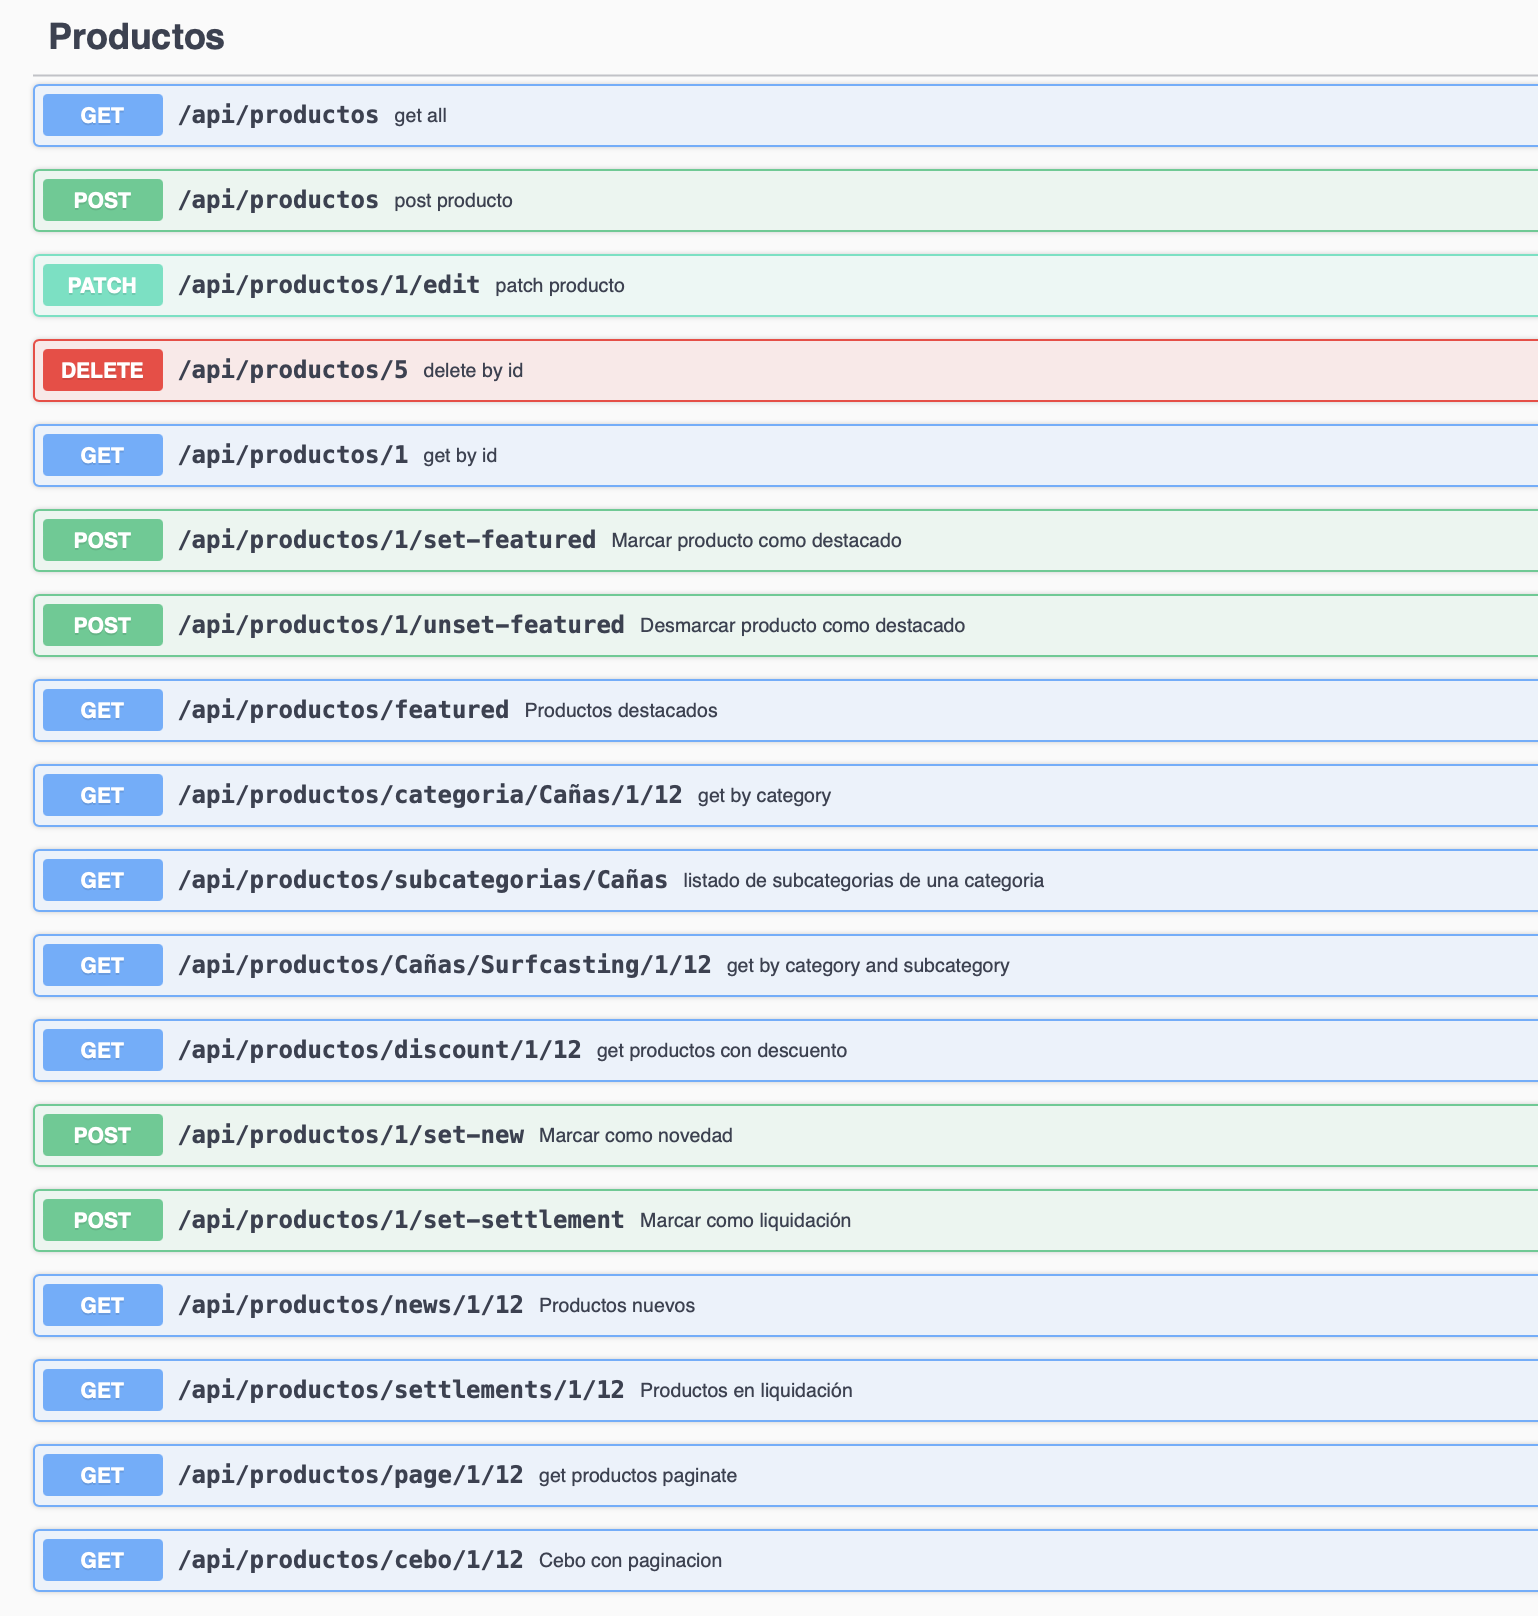
\includegraphics[scale=0.6]{./Images/APIproductos.png}
\caption{APIs de productos} Fuente: Elaboración propia.

\label{fig:fig1}

\end{center}
\end{figure}

\begin{figure}[H]
\begin{center}
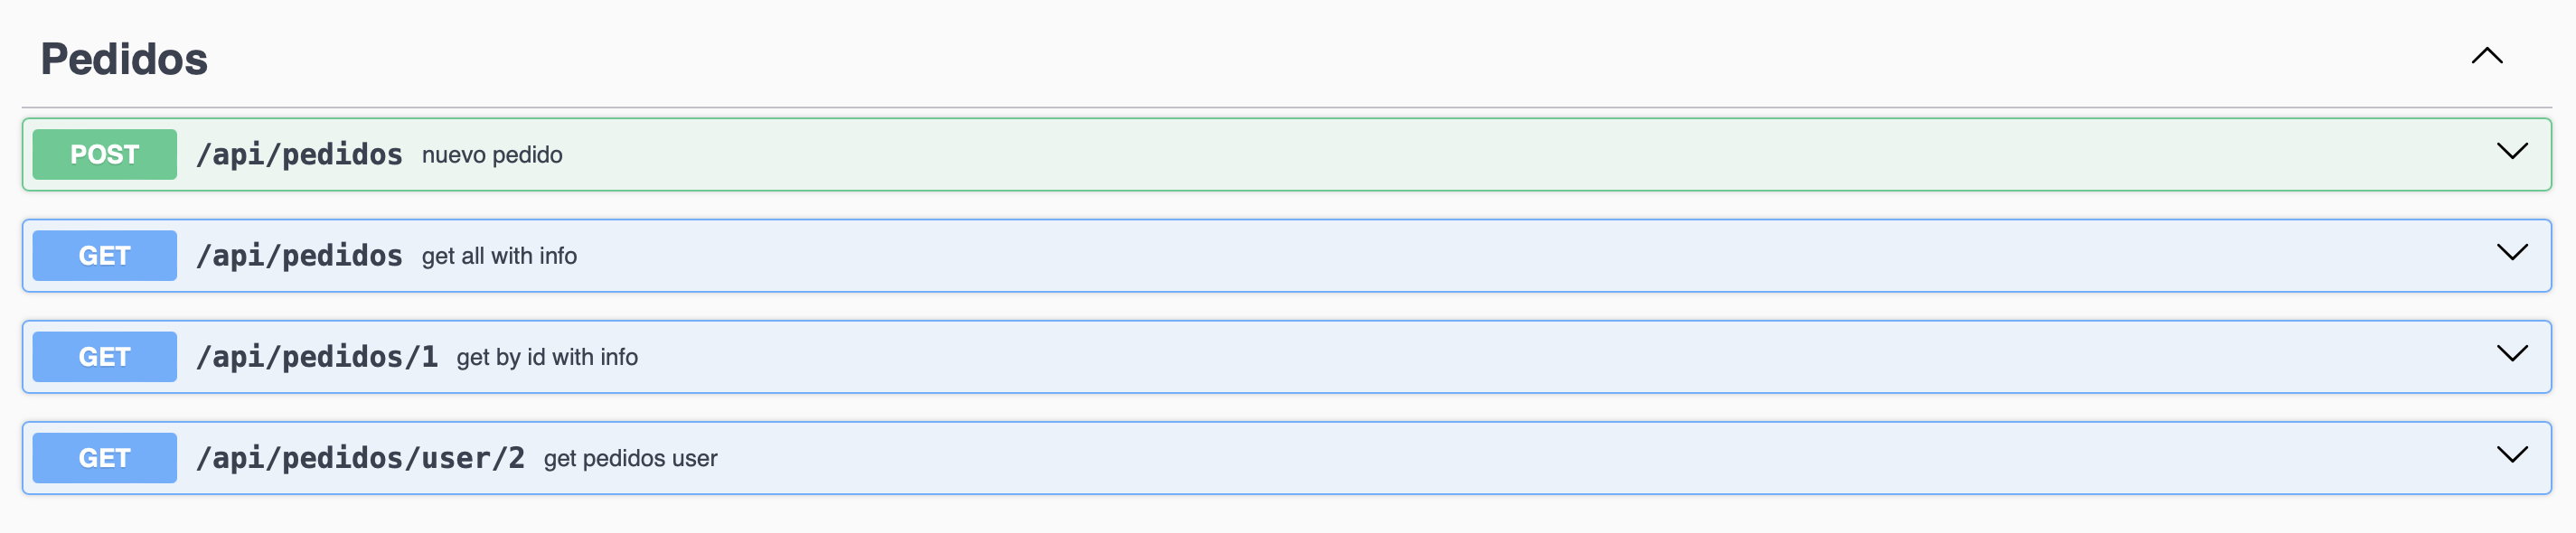
\includegraphics[scale=0.7]{./Images/APIpedidos.png}
\caption{APIs de pedidos} Fuente: Elaboración propia.

\label{fig:fig2}

\end{center}
\end{figure}

\begin{figure}[H]
\begin{center}
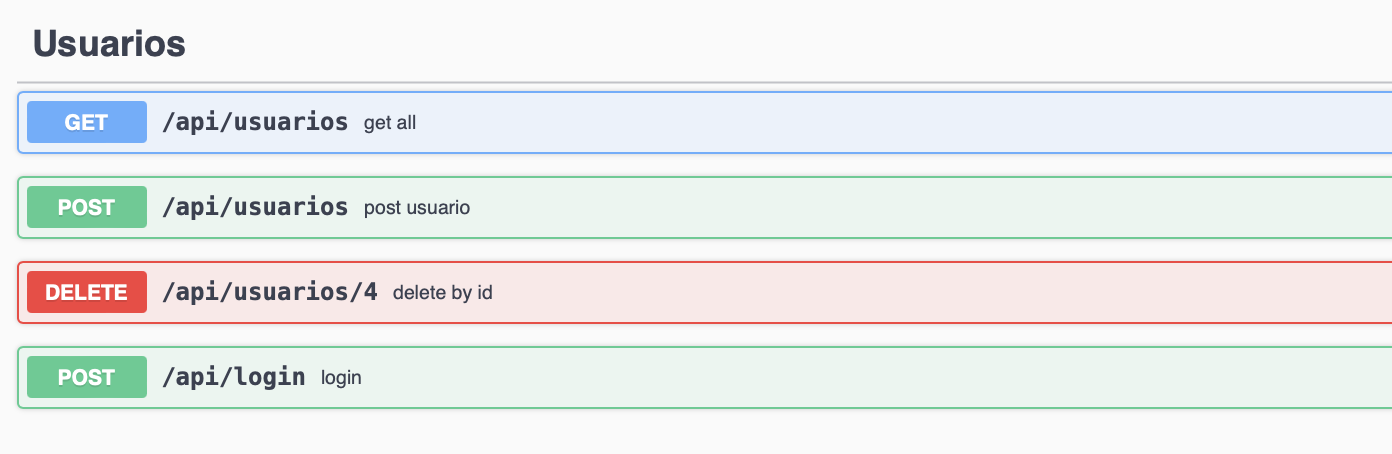
\includegraphics[scale=0.7]{./Images/APIusuarios.png}
\caption{APIs de usuarios} Fuente: Elaboración propia.

\label{fig:fig3}

\end{center}
\end{figure}

\begin{figure}[H]
\begin{center}
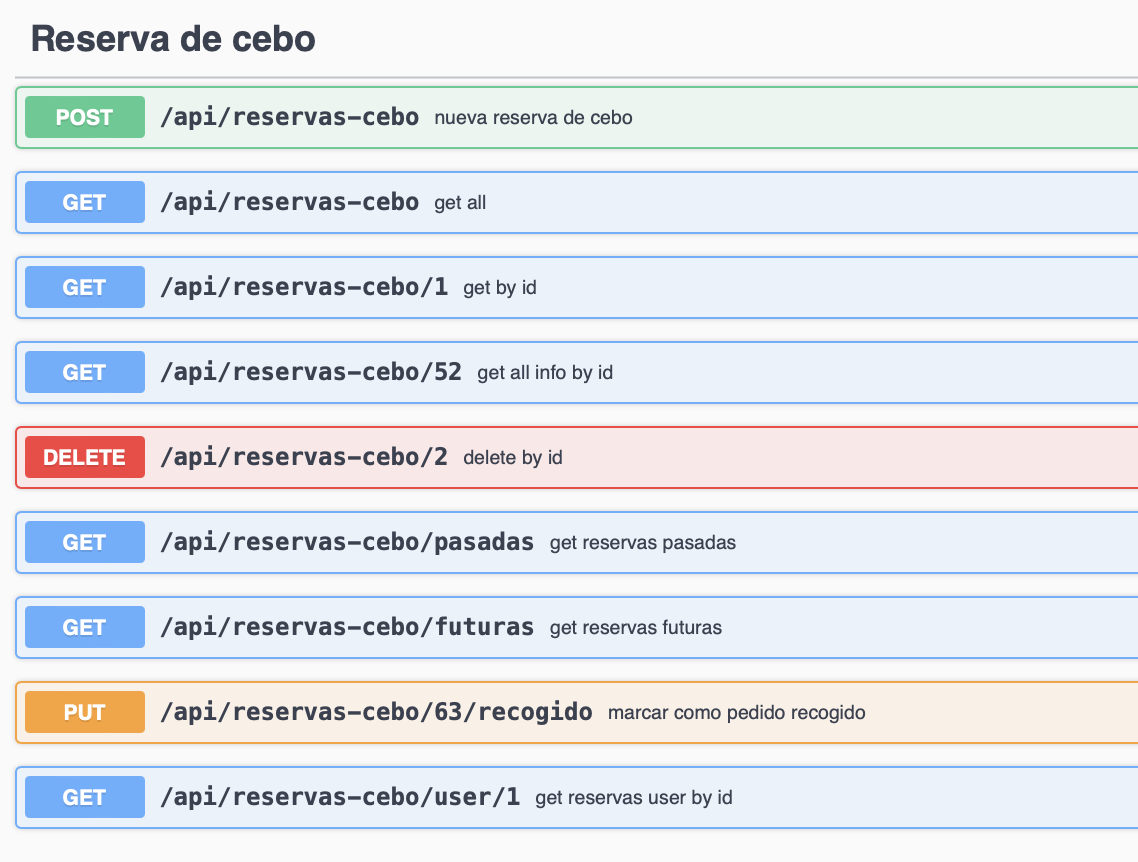
\includegraphics[scale=0.7]{./Images/APIreservacebo.png}
\caption{APIs de reserva de cebo} Fuente: Elaboración propia.

\label{fig:fig4}

\end{center}
\end{figure}

\begin{figure}[H]
\begin{center}
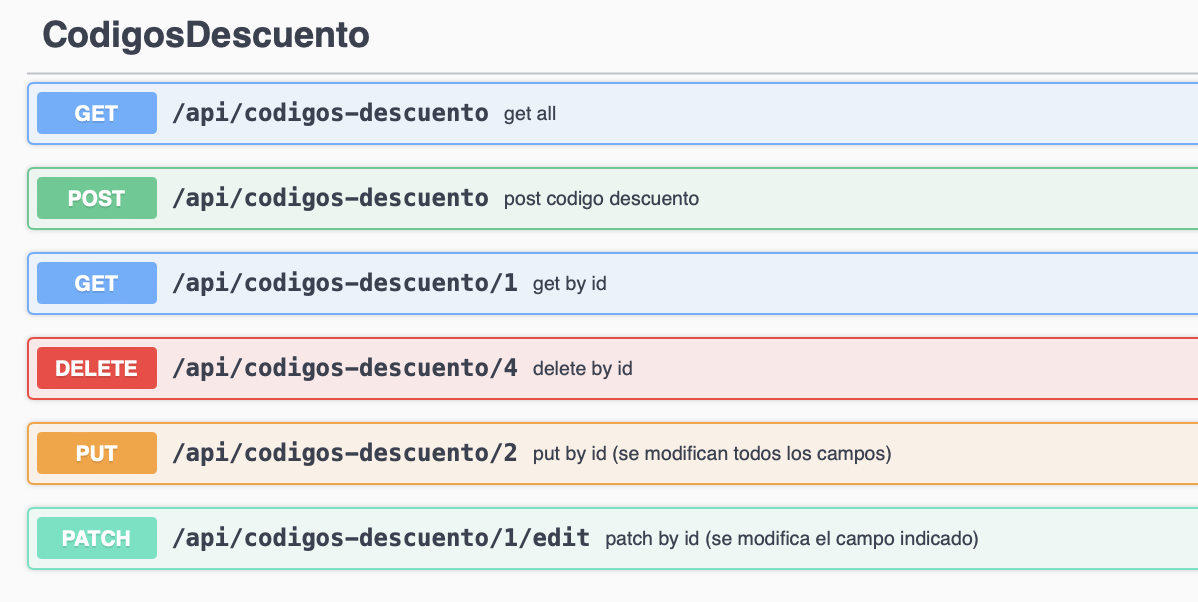
\includegraphics[scale=0.7]{./Images/APIcodigodescuento.png}
\caption{APIs de código de descuento} Fuente: Elaboración propia.

\label{fig:fig5}

\end{center}
\end{figure}

\begin{figure}[H]
\begin{center}
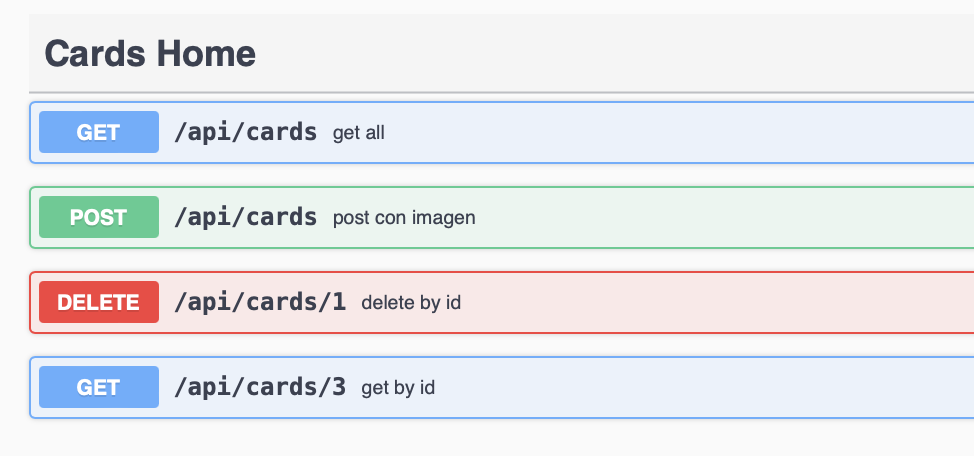
\includegraphics[scale=0.8]{./Images/APIcardshome.png}
\caption{APIs de cards de la home} Fuente: Elaboración propia.

\label{fig:fig6}

\end{center}
\end{figure}

\begin{figure}[H]
\begin{center}
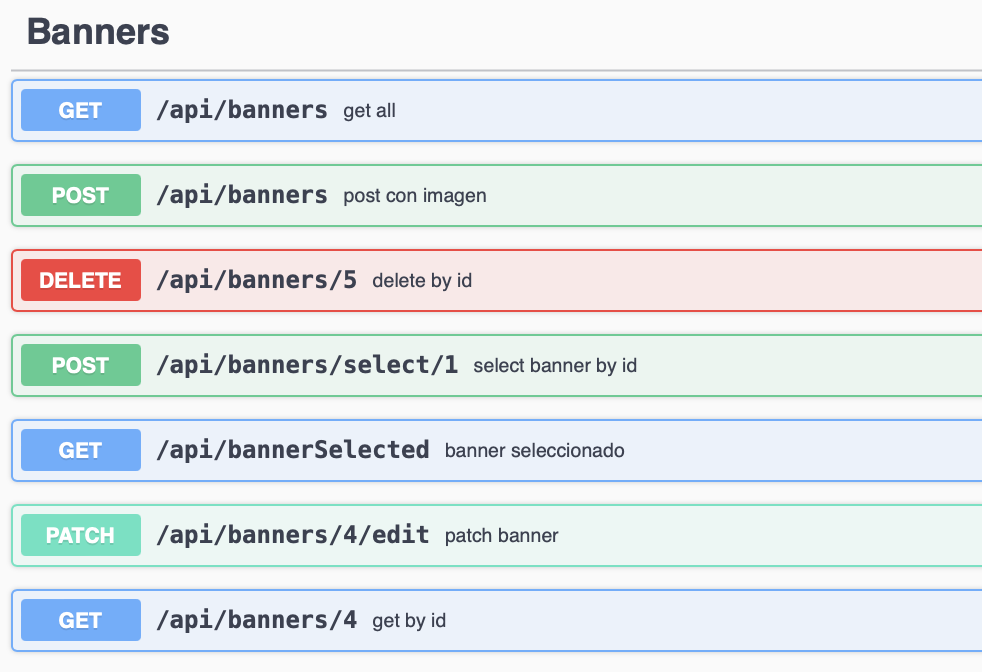
\includegraphics[scale=0.8]{./Images/APIbanners.png}
\caption{APIs banners} Fuente: Elaboración propia.

\label{fig:fig7}

\end{center}
\end{figure}

\begin{figure}[H]
\begin{center}

\includegraphics[scale=0.9]{./Images/APIciudades.png}
\caption{API ciudades} Fuente: Elaboración propia.

\label{fig:fig8}

\end{center}
\end{figure}

\begin{figure}[H]
\begin{center}

\includegraphics[scale=0.8]{./Images/APIcontacto.png}
\caption{API contacta con nosotros} Fuente: Elaboración propia.

\label{fig:fig9}

\end{center}
\end{figure}


%\
\chapter{Metodología}\label{cap:cap4}
Para afrontar este Trabajo de Fin de Máster (TFM), se ha decidido adoptar una metodología ágil que se ajusta a las exigencias dinámicas del proyecto. Esta elección se sustenta en la necesidad de asegurar una ejecución eficiente, flexible y orientada a la obtención de resultados concretos.

\vspace{0.5cm}

La metodología ágil se caracteriza por su enfoque iterativo e incremental, lo que permite dividir el proyecto en etapas o iteraciones manejables. Cada iteración se centra en un conjunto específico de tareas y objetivos, facilitando así un progreso continuo y una rápida adaptación a los cambios del entorno. Asimismo, fomenta una estrecha colaboración con los interesados y la posibilidad de realizar ajustes según las necesidades emergentes.

\vspace{0.5cm}

Es bien sabido que este enfoque ágil es altamente efectivo en proyectos de desarrollo de software, como el presente, debido a su capacidad para mejorar la gestión del proyecto. En este tipo de iniciativas, la comunicación fluida, la capacidad de adaptación y la entrega incremental de funcionalidades son aspectos cruciales. Todos estos aspectos pueden ser alcanzados eficazmente mediante la implementación de una metodología ágil.

\vspace{0.5cm}

A continuación, se detallará la gestión del proyecto y las herramientas utilizadas para su ejecución efectiva.

\section{Gestión del proyecto}\label{sec:apartado}

Para gestionar eficazmente el proyecto, se han empleado herramientas alineadas con la metodología ágil Scrum \cite{schwaber2017}. A partir de los requisitos del proyecto, se ha elaborado un Product Backlog que incluye las Historias de Usuario \cite{cohn2004}, delineando así las necesidades específicas desde la perspectiva del cliente o usuario final. En lugar de detallar exhaustivamente especificaciones técnicas, las Historias de Usuario se centran en los objetivos y expectativas de los usuarios de la aplicación.

\vspace{0.5cm}

La planificación se ha estructurado en diferentes Sprints, cada uno con las tareas necesarias para avanzar hacia el objetivo final: la aplicación web. La conclusión exitosa de estos Sprints conducirá al resultado deseado.

\vspace{0.5cm}

En la sección \textcolor{naranja}{sección 4.1.1 - Historias de usuario}, se presenta en detalle esta hoja de ruta, que guiará la creación de las funcionalidades requeridas por los usuarios, abordando así las necesidades específicas del proyecto.


\subsection{Historias de usuario}\label{subsec4.1.1}

En base a los requisitos de la aplicación se han identificado las siguientes historias de usuario:



\begin{table}[H]
  \centering
  \renewcommand{\arraystretch}{1.5}
  \begin{tabular}{|p{0.3\textwidth}|p{0.3\textwidth}|p{0.3\textwidth}|}
    \hline
    \multicolumn{3}{|l|}{\cellcolor{OrangeVIU}\textcolor{white}{\textbf{(H1) Historia de usuario 1: Creación BBDD}}} \\
    \hline
    \multicolumn{3}{|p{\dimexpr0.9\linewidth+2\tabcolsep+2\arrayrulewidth}|}{{\textbf{\textcolor{naranja}{Descripción: }}}Crear una base de datos desde cero para almacenar datos esenciales del sistema.} \\
    \hline
    \multicolumn{3}{|p{\dimexpr0.9\linewidth+2\tabcolsep+2\arrayrulewidth}|}{{\textbf{\textcolor{naranja}{Validación: }} Se debe verificar que todas las tablas requeridas hayan sido creadas correctamente en la base de datos, asegurando que cada tabla contenga las columnas necesarias y cumpla con las restricciones de integridad definidas. }} \\
    \hline
    {\textbf{\textcolor{naranja}{Prioridad }}}  & {\textbf{\textcolor{naranja}{Estimación }}}  & {\textbf{\textcolor{naranja}{Dependencia }}}  \\
    \hline
    1 &  30h &  Ninguna \\
    \hline
  \end{tabular}
  \caption{(H1) Historia de usuario 1 - Creación BBDD}
  \label{table:H1}
\end{table}


    Esta historia de usuario representa una de las primeras tareas clave en el desarrollo del sistema, que es la creación de la base de datos (BBDD). El desarrollo se ha gestionado mediante un enfoque iterativo y basado en Scrum. La creación de la base de datos es un paso crucial en la arquitectura de la aplicación, ya que asegura que toda la información requerida por el sistema esté correctamente estructurada.

    \vspace{0.5cm}
    
    La validación de esta tarea se llevará a cabo al finalizar el Sprint correspondiente, verificando la integridad de las tablas y asegurando que se cumplan los requisitos establecidos en las historias de usuario dependientes. Esta historia se considera de alta prioridad debido a su impacto en las demás funcionalidades del sistema.


\begin{table}[H]
  \centering
  \renewcommand{\arraystretch}{1.5}
  \begin{tabular}{|p{0.3\textwidth}|p{0.3\textwidth}|p{0.3\textwidth}|}
    \hline
    \multicolumn{3}{|l|}{\cellcolor{OrangeVIU}\textcolor{white}{\textbf{(H2) Historia de usuario 2: Introducir nuevo producto}}} \\
    \hline
    \multicolumn{3}{|p{\dimexpr0.9\linewidth+2\tabcolsep+2\arrayrulewidth}|}{{\textbf{\textcolor{naranja}{Descripción: }}}Permitir a los usuarios agregar un nuevo producto al sistema, proporcionando información detallada como nombre, descripción, precio y categoría.} \\
    \hline
    \multicolumn{3}{|p{\dimexpr0.9\linewidth+2\tabcolsep+2\arrayrulewidth}|}{{\textbf{\textcolor{naranja}{Validación: }} Verificar que el nuevo producto se haya añadido correctamente a la base de datos, con todos los campos necesarios completos y sin errores de duplicación. }} \\
    \hline
    {\textbf{\textcolor{naranja}{Prioridad }}}  & {\textbf{\textcolor{naranja}{Estimación }}}  & {\textbf{\textcolor{naranja}{Dependencia }}}  \\
    \hline
    1 &  10h &  1 \\
    \hline
  \end{tabular}
  \caption{(H2) Historia de usuario 2 - Introducir nuevo producto}
  \label{table:H2}
\end{table}


    Esta historia de usuario aborda la funcionalidad esencial para el administrador de la aplicación, permitiéndole gestionar el catálogo de productos en el sistema. El enfoque Scrum nos ha permitido dividir esta tarea en sub-actividades como el diseño de la interfaz de usuario, la conexión con la base de datos y la validación de datos.

    \vspace{0.5cm}
    
    Durante el Sprint, se llevarán a cabo pruebas unitarias y de integración para garantizar que el sistema maneje correctamente la introducción de nuevos productos y que los datos se guarden de manera segura en la base de datos. Esta tarea es crítica para garantizar que el inventario se mantenga actualizado en todo momento, siendo una funcionalidad recurrente en futuras iteraciones.


\vspace{0.5cm}
\vspace{0.5cm}
Después de presentar las primeras historias de usuario clave para el desarrollo del sistema, el resto de las historias de usuario, que detallan el resto de funcionalidades se encuentran recogidas en el \textcolor{naranja}{Anexo I: Historias de usuario}. Estas historias son igualmente importantes para la correcta implementación y funcionamiento de la plataforma, y abarcan aspectos como la gestión avanzada del inventario, la autenticación de usuarios y la reserva de productos. Para mayor detalle, se pueden consultar todas las tablas en el mencionado anexo.







\renewcommand{\bibname}{Bibliografía}
\bibliographystyle{apacite}
%\bibliographystyle{alpha}
\bibliography{biblio}



\end{document}
